% !TEX TS-program = pdflatex
% !TEX encoding = UTF-8 Unicode

% This is a simple template for a LaTeX document using the "article" class.
% See "book", "report", "letter" for other types of document.

\documentclass[12pt, titlepage]{article} % use larger type; default would be 10pt

\usepackage[utf8]{inputenc} % set input encoding (not needed with XeLaTeX)

%%% Examples of Article customizations
% These packages are optional, depending whether you want the features they provide.
% See the LaTeX Companion or other references for full information.

%%% PAGE DIMENSIONS
\usepackage{geometry} % to change the page dimensions
\geometry{a4paper} % or letterpaper (US) or a5paper or....
% \geometry{margin=2in} % for example, change the margins to 2 inches all round
% \geometry{landscape} % set up the page for landscape
%   read geometry.pdf for detailed page layout information

\usepackage{graphicx} % support the \includegraphics command and options

% \usepackage[parfill]{parskip} % Activate to begin paragraphs with an empty line rather than an indent

%%% PACKAGES
\usepackage[usenames,dvipsnames,svgnames,table]{xcolor}
\usepackage{csvsimple}
\usepackage[hyphens]{url}
\usepackage{booktabs} % for much better looking tables
\usepackage{array} % for better arrays (eg matrices) in maths
\usepackage{paralist} % very flexible & customisable lists (eg. enumerate/itemize, etc.)
\usepackage{verbatim} % adds environment for commenting out blocks of text & for better verbatim
%\usepackage{subfig} % make it possible to include more than one captioned figure/table in a single float
\usepackage{tabu}
\usepackage{tabularx}
\usepackage{float}
\usepackage[utf8]{inputenc}
\usepackage[export]{adjustbox}[2011/03/20]
\usepackage{color}
\usepackage{caption}
\usepackage{subcaption}
\usepackage{comment} % Takashi added the package on 2016/12/21
% These packages are all incorporated in the memoir class to one degree or another...

%%% HEADERS & FOOTERS
\usepackage{fancyhdr} % This should be set AFTER setting up the page geometry
\pagestyle{fancy} % options: empty , plain , fancy
\renewcommand{\headrulewidth}{0pt} % customise the layout...
\lhead{}\chead{}\rhead{}
\lfoot{}\cfoot{\thepage}\rfoot{}

%%% SECTION TITLE APPEARANCE
\usepackage{sectsty}
%\allsectionsfont{\sffamily} % (See the fntguide.pdf for font help)

%%% ToC (table of contents) APPEARANCE
\usepackage[nottoc,notlof,notlot]{tocbibind} % Put the bibliography in the ToC
\usepackage[titles,subfigure]{tocloft} % Alter the style of the Table of Contents
\renewcommand{\cftsecfont}{\rmfamily\mdseries\upshape}
\renewcommand{\cftsecpagefont}{\rmfamily\mdseries\upshape} % No bold!

%%% END Article customizations

%%% THE REAL DOCUMENT BEGINS NOW!!!


%%%%%%%%%%%%%%%%%%%%%%%%%%%%%%%%%%%%%%%%%%%%%%%%%%%%%%%%%%%%%%%%%%%%%%


\title{LiteBIRD Sensitivity Calculation \\ Version 22}
\author{Charles Hill \\ with Tomotake Matsumura, Aritoki Suzuki,  \\ Kam Arnold, Johannes Hubmayr, \\ Yuto Minami and Takashi Hasebe}
\date{2016-12-21} % Activate to display a given date or no date (if empty),
         % otherwise the current date is printed 

\begin{document}
\maketitle

%%%%%%%%%%%%%%%%%%%%%%%%%%%%%%%%%%%%%%%%%%%%%%%%%%%%%%%%%%%%%%%%%%%%%%

\clearpage

\begin{center}
\fontsize{24}{12}
\textbf{Revision History}  \\
\vspace{10mm}
\end{center}
\fontsize{12}{12}

New in Version 22
\begin{itemize}
	\item Modified the equation for mirror efficiency
	\item Added the comment for the sapphire index in Table 18 
\end{itemize}

New in Version 21
\begin{itemize}
	\item Careful readthrough of text, getting ready to hand off to Tomo, Yuto, and Takashi
	\item Updating tables, figures, and text to represent what we presented in the CSR
\end{itemize}

New in Version 20
\begin{itemize}
	\item Updated sensitivity values
	\item Updated detector count, wafer distributions, optical element assumptions, NEP values, NET margin, etc.
	\item This version essentially syncs up with the CSR
\end{itemize}

New in Version 11
\begin{itemize}
	\item Modification to the extreme loading scenarios from a baffle temperature of 4.5K and 6.0K (formerly 1.5K and 6.0K)
	\item Introduction of Section 9.2 which plots both band-by-band and overall sensitivity vs the temperature of various optical elements
\end{itemize}

New in Version 10
\begin{itemize}
	\item Bug fix in TeX table handling that has changed the following items
		\begin{itemize}
			\item Table 1: Public vs this document
			\item Table 19: Sensitivity with margin
		\end{itemize}
\end{itemize}

New in Version 9
\begin{itemize}
	\item Bolometer thermal carrier changed from electron to phonon
	\item Band center frequencies rounded to nearest GHz
	\item Upgrades to pixel diameter optimization
		\begin{itemize}
			\item Presentation of pixel optimization for both reflection to baffle and reflection to focal plane
			\item More transparent explanations behind pixel number quantization and limits on pixel size for each frequency band
		\end{itemize}
	\item Added Section \ref{sec:possibleLoadings} to show range of possible in-band loading values for each frequency channel	
\end{itemize}

New in Version 8
\begin{itemize}
	\item Comparision of public in-band loading vs that of this document
	\item Explicit list of differences between public sensitivity calculation and that of this document
	\item Minor bug fix in handling of HFT reflections
\end{itemize}

New in Version 7
\begin{itemize}
	\item Added "Opening Remark" that presents the public uK-armin values from Tomo's LTD proceeding adjacent to the uK-arcmin values calculated in this document
\end{itemize}

New in Version 6
\begin{itemize}
	\item Explicit calculation of frequency dependencies in the system 
	\item Explicit handling of reflections landing on temperatures other than that of the focal plane
	\item Transparent presentation of all assumptions behind emissivity and efficiency values of every optical element
\end{itemize}

%%%%%%%%%%%%%%%%%%%%%%%%%%%%%%%%%%%%%%%%%%%%%%%%%%%%%%%%%%%%%%%%%%%%%%
\iffalse
\clearpage

\begin{center}
\fontsize{24}{12}
\textbf{Opening Remark}  \\
\vspace{10mm}
\fontsize{12}{12}
The sensitivity values presented in this document are \textbf{not public}. For the latest public values, please refer to Tomotake Matsumura's 2015 Low Temperature Detector (LTD) Conference proceedings. For reference, I have displayed Tomo's sensitivity values next to the values calculated in this document in the table below. Note that NET Array values are with no margin for yield, NET contingency, etc. while the listed sensitivity values do include contingency factors.
\end{center}

\begin{table}[H]
\centering
	\begin{tabu}{|| c || c | c | c || c | c | c ||}
	\hline
	& \multicolumn{3}{c ||}{\textbf{Public Values}} & \multicolumn{3}{c ||}{\textbf{This Document}} \\
	\hline
	\hline
	Band & Loading & $\mathrm{NET_{Arr}}$ & Sensitivity & Loading & $\mathrm{NET_{Arr}}$ & Sensitivity \\
	 & [pW] & $\mathrm{[\mu K\sqrt{sec}]}$ & $\mathrm{[\mu K-arcmin]}$ & [pW] & $\mathrm{[\mu K\sqrt{sec}]}$ & $\mathrm{[\mu K-arcmin]}$ \\
	\hline
	\csvreader[ late after line = \\ \hline, late after last line =]{CSV/openingRemark.csv}{}{\a & \b & \c & \d & \e & \f & \g}
	\csvreader[head to column names, late after line = \\ \hline]{CSV/openingRemarkTotal.csv}{}{\\ \hline \multicolumn{1}{||c||}{\a} & \multicolumn{1}{c}{} & \multicolumn{1}{c}{} & \multicolumn{1}{c ||}{\b} & \multicolumn{1}{c}{} & \multicolumn{1}{c}{} & \multicolumn{1}{c||}{\c}}
	%\csvreader[head to column names, late after line = \\ \hline]{CSV/openingRemarkCMBTotal.csv}{}{\\ \hline \multicolumn{1}{||c||}{\a} & \multicolumn{1}{c}{} & \multicolumn{1}{c}{} & \multicolumn{1}{c ||}{\b} & \multicolumn{1}{c}{} & \multicolumn{1}{c}{} & \multicolumn{1}{c||}{\c}}
	\end{tabu}
\caption{Public sensitivies compared against those calculated in this document}
\end{table}

In the table below, I've listed all of the changes to the sensitivity calculation since the last-released public version, and I've listed each change's fractional impact on the overall sensitivity number with margin (listed as 3.2 $\mathrm{ \mu K - arcmin }$ ). In other words, we use the equation

\begin{equation}
	\mathrm{Fractional \; Impact} = \frac{(\mathrm{This \; Document}) - (\mathrm{Public})}{\mathrm{Public}}
\end{equation}

\begin{table}[H]
\centering
	\begin{tabularx}{\textwidth}{|| X | X | X | X ||}
	\hline
	\textbf{Introduced} & \textbf{Public} & \textbf{This Document} & \textbf{Frac Diff} \\
	\hline
	\hline
	Ver 6 & Assume 0.5\% mirror absorption & Calculate mirror absorption using Equation \ref{eq:ohmicLoss} & -1.9\% \\
	\hline
	Ver 6 & Assume 0.1\% mirror scattering & Calculate mirror scattering using Eqaution \ref{eq:ruzeLoss} & 0.0 \% \\
	\hline
	Ver 6 & Assume all reflections go back to 100mK focal plane & Explicitly specify what temperature relfections land on for each optical element & +16\% \\
	\hline
	Ver 7 & Assume 10\% reflection from LFT  Filter & Assume 5\% reflection from LFT 2 K Filter & -2.2\% \\
	\hline
	Ver 7 & Assume 2\% reflection from HFT 2 K Filter & Assume 5\% reflection from HFT 2 K Filter & 0.0\% \\
	\hline
	Ver 9 & HF-1 diameter 5.2mm, HF-3 diamter 3.8mm, n = 1, $\mathrm{T_{c}} = 0.214 K$ & HF-1 diameter 5.4mm, HF-3 diamter 4.0mm, n = 3, $\mathrm{T_{c}} = 0.171 K$ & +3.1 \% \\
	\hline
	\end{tabularx}
\caption{Differences between public sensitivity calculation and the sensitivity calculation layed out in this document}
\end{table}

	 

Note that the difference the public sensitivity and that presented in this document is driven by the handling of reflection. Tomo's proceding assumes that all reflected radiation lands on the 100mK focal plane, while my calculation assumes that most refelcted radiation lands on the 5K baffling. Reality will fall somewhere between these two extremes...

\clearpage
\fi
%%%%%%%%%%%%%%%%%%%%%%%%%%%%%%%%%%%%%%%%%%%%%%%%%%%%%%%%%%%%%%%%%%%%%%

\tableofcontents
\newpage


%%%%%%%%%%%%%%%%%%%%%%%%%%%%%%%%%%%%%%%%%%%%%%%%%%%%%%%%%%%%%%%%%%%%%%


\section{Experimental Design Overview}

This section outlines the basic aspects of the LiteBIRD instrument that are important to our sensitivity estimate.

\subsection{Observing Parameters}

This document assumes the observing parameters displayed in Table \ref{table:LbParams}.

\begin{table}[H]
\centering
	\begin{tabu}{|| c | c ||}
	\hline
	Parameter & Value \\
	\hline
	\hline
	Sky Fraction & 1.0 \\ 
	\hline
	Observing Time & 3 years \\
	\hline
	\end{tabu}
\caption{Observing parameters \label{table:LbParams}}
\end{table}

Note that we take $\mathrm{f_{sky}}$ to be 1.0 because LiteBIRD is a full-sky survey. 

%%%%%%%%%%%%%%%%%%%%%%%%%%%%%%%%%%%%%

\subsection{Low Frequency Telescope Focal Plane Specifications}

Figure \ref{fig:lftFP} is Ted Kisner's drawing of the Low Frequency Telescope (LFT) focal plane, with a color coding scheme to show where each frequency channel lies within the detector array. Table \ref{table:lftParams} provides the parameters of the frequency channels on the LFT focal plane. Note how the choice pixel size and the fact we are using 6-inch hexagonal wafers determines the number of detectors in each frequency channel.

\begin{figure}[h!]
	\centering
	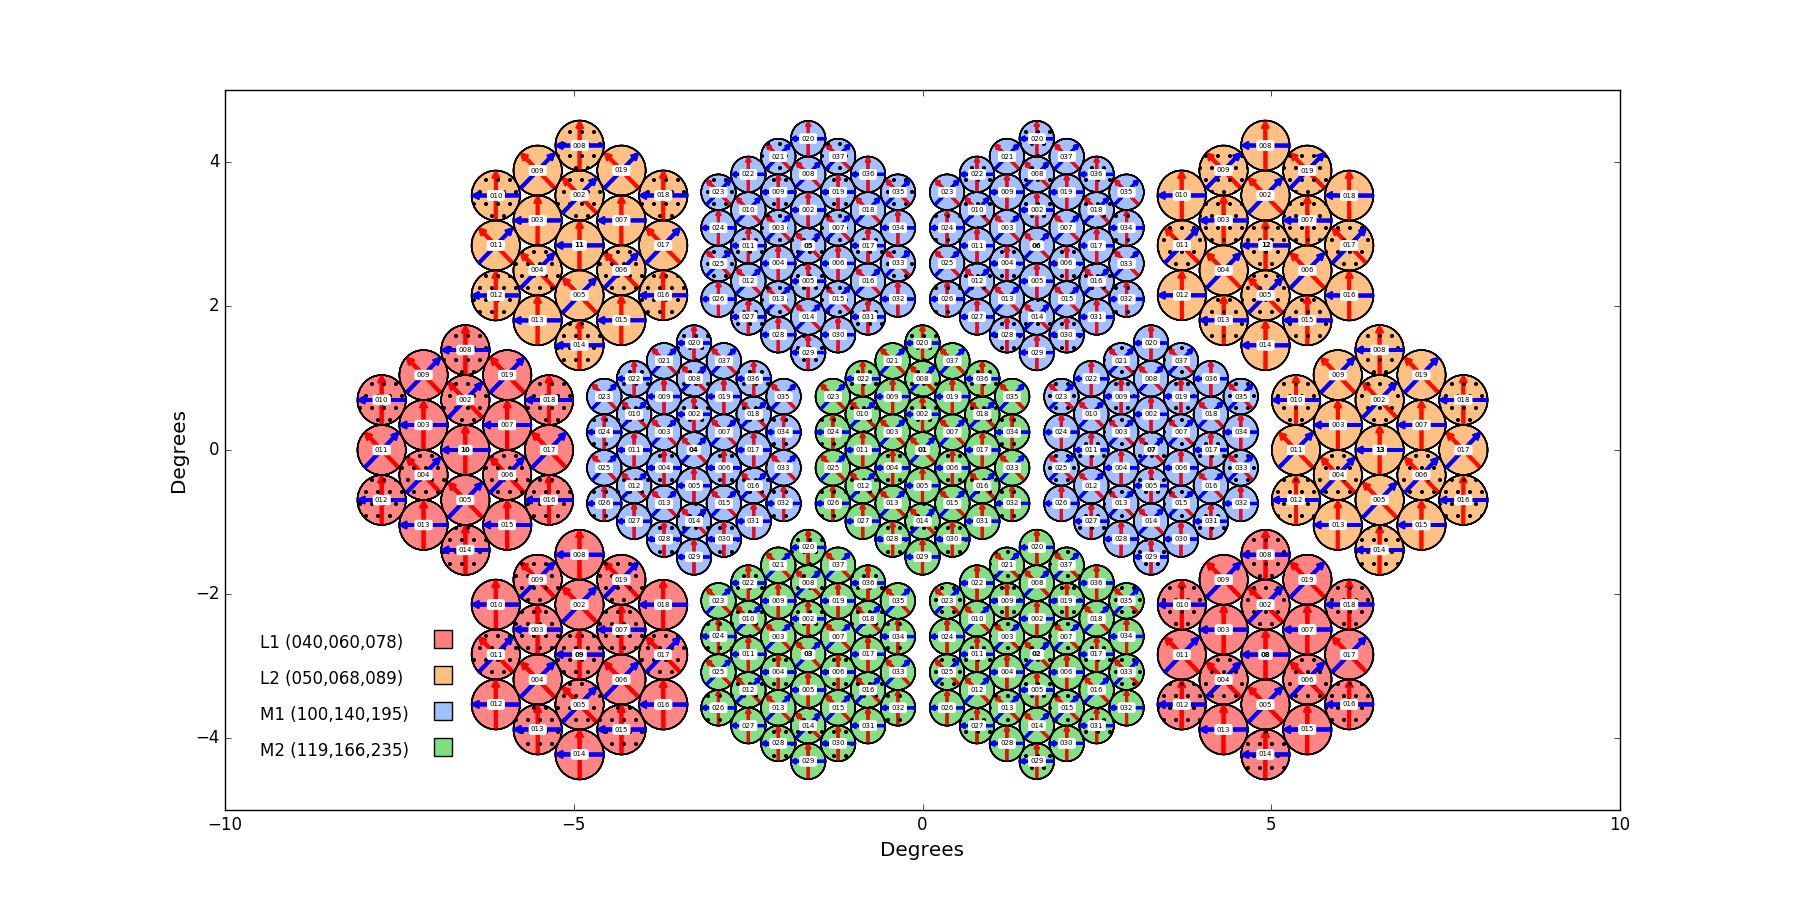
\includegraphics[trim={10.0cm, 0.0cm, 10.0cm, 0.0cm}, width=0.8\textwidth]{PNG/LFT_Ted.png}
	\caption{LFT focal plane with wafers color-coded to highlight the location of the corresponding frequency channels \label{fig:lftFP}}
\end{figure}

\begin{table}[H]
\centering
	\begin{tabu}{|| c | c | c | c | c | c ||}
	\hline
	Band & Center Freq & Frac BW & Pixel Diameter & Num Pix & Num Det \\
	 &  [GHz] & & [mm] & & \\
	\hline \hline
	\rowfont{\color{red}}
		LF-1 & 40 & 0.30 & 18 & 57 & 114 \\
	\hline
	\rowfont{\color{orange}}
		LF-2 & 50 & 0.30 & 18 & 57 & 114 \\
	\hline
	\rowfont{\color{Red}}	
		LF-3 & 60	 & 0.23 & 18 & 57 & 114 \\
	\hline
	\rowfont{\color{Orange}}
		LF-4 & 68 	& 0.23 & 18 & 57 & 114 \\
	\hline
	\rowfont{\color{Red}}
		LF-5 & 78	 & 0.23 & 18 & 57 & 114 \\
	\hline
	\rowfont{\color{Orange}}
		LF-6 & 89 & 0.23 & 18 & 57 & 114 \\
	\hline
	\rowfont{\color{Blue}}
		MF-1 & 100 & 0.23 & 12 & 148 & 296 \\
	\hline	
	\rowfont{\color{Green}}
		MF-2 & 119 & 0.30 & 12 & 111 & 222 \\
	\hline
	\rowfont{\color{Blue}}
		MF-3 & 140 & 0.30 & 12 & 148 & 296 \\
	\hline
	\rowfont{\color{Green}}	
		MF-4 & 166 & 0.30 & 12 & 111 & 222 \\
	\hline
	\rowfont{\color{Blue}}	
		MF-5 & 195 & 0.30 & 12 & 148 & 296 \\
	\hline
	\rowfont{\color{Green}}
		MF-6 & 235 & 0.30 & 12 & 111 & 222 \\
	\hline
	\end{tabu}
\caption{Frequency channels of the LFT color-coded to highlight the position of each channel on the focal plane \label{table:lftParams}}
\end{table}

%%%%%%%%%%%%%%%%%%%%%%%%%%%%%%%%%%%%%

\subsection{High Frequency Telescope Focal Plane Specifications}

The High Frequency Telescope (HFT) focal plane is an array of monochroic, horn-coupled, orthomode transducers (OMTs) covering three frequencies shown by Hannes Hubmayr's drawing in Figure \ref{fig:hftFP}. The parameters of each frequency channel are given in Table \ref{table:hftParams}. For the HFT, while the pixel sizes are optimized (see Section \ref{sec:pixOpt}), the number of detectors is not at the moment. In other words, we may be able to add more detectors by packing the focal plane more densely. Whether or not this is possible or advisable relies on telemetry and crosstalk requirements.

\begin{figure}[h!]
	\centering
	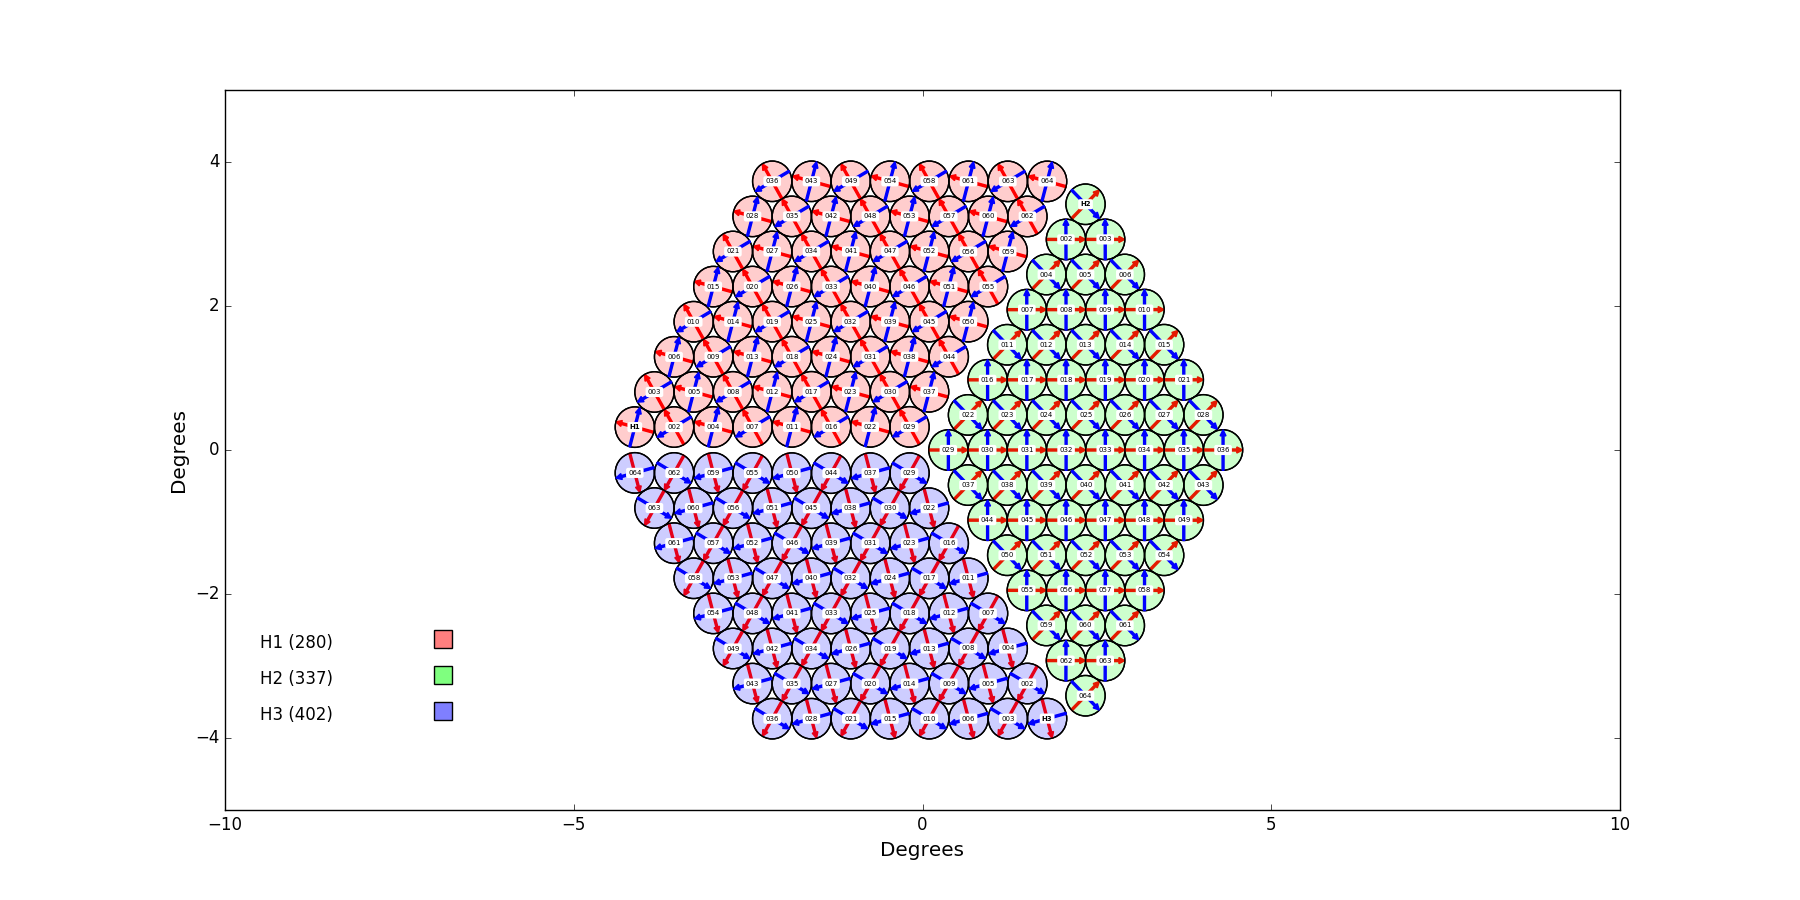
\includegraphics[trim={10.0cm, 1.0cm, 10.0cm, 0.0cm}, width=0.8\textwidth]{PNG/HFT_Ted.png}
	\caption{HFT focal plane with detectors color-coded to highlight the location of the corresponding frequency channels \label{fig:hftFP}}
\end{figure}

\begin{table}[h!]
\centering
	\begin{tabu}{|| c | c | c | c | c | c ||}
	\hline
	Band & Center Freq & Frac BW & Pixel Diameter & Num Pix & Num Det \\
	 & [GHz] & & [mm] & & \\
	\hline \hline
	\rowfont{\color{Red}}
	HF-1 & 280 & 0.30 & 5.4 & 64 & 128 \\
	\hline
	\rowfont{\color{Green}}
	HF-2 & 337 & 0.30 & 4.5 & 64 & 128 \\
	\hline
	\rowfont{\color{Blue}}	
	HF-3 & 402 & 0.23 & 4.0 & 64 & 128 \\
	\hline
	\end{tabu}
\caption{Frequency channels of the HFT \label{table:hftParams}}
\end{table} 

%%%%%%%%%%%%%%%%%%%%%%%%%%%%%%%%%%%%%

\subsection{Detector Parameters}

Table 4 shows the assumptions that we take regarding detector design when calculating noise performance.

\begin{table}[H]
\centering
	\begin{tabular}{|| c | c ||}
	\hline
	Parameter & Assumed Value \\
	\hline
	\hline
	Bath Temperature [K] & 0.100 \\ 
	\hline
	Transition Temperature [K] & 0.171 \\
	\hline
	Thermal Carrier & Phonon (n = 3) \\
 	\hline
	$\mathrm{P_{oper}/P_{opt}}$ & 2.5 \\
	\hline
	\end{tabular}
\caption{Table of detector parameters}
\end{table}

Note that $\mathrm{P_{oper}}$ is the operating power of the bolometer and is calculated as

\begin{equation}
	\mathrm{P_{oper} = P_{opt} + P_{elec}}
\end{equation}

where $\mathrm{P_{opt}}$ and $\mathrm{P_{elec}}$ are the optical power and electrical power on the bolometer, respectively.

%%%%%%%%%%%%%%%%%%%%%%%%%%%%%%%%%%%%%%%%%%%%%%%%%%%%%%%%%%%%%%%%%%%%%%

\newpage

\section{Overview of Noise Sources}

For LiteBIRD, we consider two categories of noise sources: internal and external.

%%%%%%%%%%%%%%%%%%%%%%%%%%%%%%%%%%%%%

\subsection{Internal Noise}

Internal noise sources are those which are inhrently tied to the fundamental operation of the detector and optics and therefore cannot be easily reduced without changes to the experimental design. The internal noise sources considered in this memo are listed in Table \ref{table:IntNoiseSources}.

\begin{table}[H]
\centering
	\begin{tabularx}{\textwidth}{|| c | c | X ||}
	\hline
	Internal Noise Source & Symbol & Description \\
	\hline \hline
	Photon Noise & $\mathrm{NEP_{ph}}$ & Noise due to the distrubution of arrival times of photons at the detector input \cite{zmuidzinas} \\
	\hline
	Thermal Carrier Noise & $\mathrm{NEP_{g}}$ & Thermal noise associated with heat transport across the bolometer legs\\ 
	\hline
	Readout Noise & $\mathrm{NEP_{read}}$ & Noise associated with fluctuations in the bias current across the bolometer\\
	\hline
	\end{tabularx}
\caption{Internal Noise Sources \label{table:IntNoiseSources}}
\end{table}

%%%%%%%%%%%%%%%%%%%%%%%%%%%%%%%%%%%%%

\subsection{External Noise}

External noise sources are those which interfere with the operation of the designe instrument and can in principle be reduced. The external noise sources considered in this memo are listed in Table \ref{table:ExtNoiseSources}. 

\begin{table}[H]
\centering
	\begin{tabularx}{\textwidth}{|| c | c | X ||}
	\hline
	External Noise Source & Symbol & Description \\
	\hline \hline
	Vibrational Noise & $\mathrm{NEP_{vib}}$ & Microphonic noise due to vibrations of the focal plane\\
	\hline
	Thermal Fluctuation & $\mathrm{NEP_{TF}}$ & Noise due to fluctuations in bath temperature \\ 
	\hline
	Cosmic Rays & $\mathrm{NEP_{CR}}$ & Noise due to TES heating caused by cosmic ray hits \\
	\hline
	Magnetic Interference & $\mathrm{NEP_{mag}}$ & Noise due to magnetic flux fluctuations across the TES \\
	\hline
	Electromagnetic Interference & $\mathrm{NEP_{EMI}}$ & Noise due to electromagnetic interference within the readout system  \\
	\hline
	\end{tabularx}
\caption{External Noise Sources \label{table:ExtNoiseSources}}
\end{table}

\textbf{It is a requirement that the external noise be subdominant to the internal noise.}


%%%%%%%%%%%%%%%%%%%%%%%%%%%%%%%%%%%%%%%%%%%%%%%%%%%%


\section{LFT Noise Calculation}

In this section, we overview the optical elements of the LFT and use their specifications to calculate LFT detector noise. 

%%%%%%%%%%%%%%%%%%%%%%%%%%%%%%%%%%%%%

\subsection{Optical Element Efficiencies}

Table \ref{table:lftOptElems} presents the assumed optical parameters for the LFT, with the sky-side-most elements first and the detector-side-most elements last.

\begin{table}[H]
\centering
	\begin{tabular}{|| c | c | c | c | c | c ||}
	\hline
	Element & $T$ [K] & $T_{r}$ [K] & $\epsilon$ & $r$ & $\eta$ \\
	\hline
	\hline
	CMB & 2.725 & 2.725 & 1.000 & 0.000 & 1.000 \\
	\hline
	HWP & 5.000 & 5.000 & $\epsilon_{LFT,HWP} (\nu)$ & 0.080 & $\eta_{LFT,HWP} (\nu)$ \\
	\hline
	Aperture Stop & 2.000 & NA & $\epsilon_{Aprt} (\nu)$ & 0.000 & $\eta_{Apert} (\nu)$ \\
	\hline
	Primary Mirror & 5.000 & 5.000 & $\epsilon_{Mirr} (\nu)$ & $r_{Mirr} (\nu)$ & $\eta_{Mirr} (\nu)$ \\
	\hline
	Secondary Mirror & 5.000 & 5.000 & $\epsilon_{Mirr} (\nu)$ & $r_{Mirr} (\nu)$ & $\eta_{Mirr} (\nu)$ \\
	\hline
	2 K Filter & 2.000 & 0.100 & $\epsilon_{2KF} (\nu)$ & 0.050 & $\eta_{2KF} (\nu)$ \\
	\hline
	Lenslet & 0.100 & 0.100 & $\epsilon_{Lenslet} (\nu)$ & 0.050 & $\eta_{Lenslet} (\nu)$ \\
	\hline
	Detector & 0.100 & 0.100 & 0.000 & 0.320 & 0.680 \\
	\hline
	\end{tabular}
\caption{LFT optical elements \label{table:lftOptElems}}
\end{table}

where $T$ is the temperature of the element, $T_{r}$ is the temperature the element reflects/scatters to, $\epsilon$ is the emissivity of the element, $r$ is the reflectivity of the element, and $\eta$ is the efficiency of the element. Note that the frequency-dependent values are calculated for each frequency band. \textbf{The assumptions and details behind these values can be reviewed in Section \ref{sec:optElemCalc}}.

%%%%%%%%%%%%%%%%%%%%%%%%%%%%%%%%%%%%%

\subsection{Internal Noise}

Table \ref{table:lftIntNoise} presents the calculated internal noise values for the LFT given the assumptions previously presented.

\begin{table}[H]
\centering
	\begin{tabular}{|| c | c | c | c | c | c | c ||}
	\hline
	Band & $\eta_{Apert}$ & $\mathrm{P_{opt}}$ & $\mathrm{NEP_{ph}}$ & $\mathrm{NEP_{g}}$ & $\mathrm{NEP_{read}}$ & $\mathrm{NEP_{int}}$ \\
	 & & [pW] & $\mathrm{[aW / \sqrt{Hz}]}$ & $\mathrm{[aW / \sqrt{Hz}]}$ & $\mathrm{[aW / \sqrt{Hz}]}$ & $\mathrm{[aW / \sqrt{Hz}]}$ \\
	\hline \hline
	\csvreader[head to column names, late after line= \\ \hline]{CSV/LFTInternalNoise.csv}{}{\a & \b & \c & \d & \e & \f & \g}
	\end{tabular}
\caption{LFT internal noise source calculations \label{table:lftIntNoise}}
\end{table}

%%%%%%%%%%%%%%%%%%%%%%%%%%%%%%%%%%%%% 

\subsection{External Noise}

Table \ref{table:lftExtNoise} presents the calculated external noise values for the LFT.  \textbf{As of 2016-12-20 these have not been calculated}.

\begin{table}[H]
\centering
	\begin{tabu}{|| c | c | c | c | c | c | c ||}
	\hline
	Band & $\mathrm{NEP_{vib}}$ & $\mathrm{NEP_{CR}}$ & $\mathrm{NEP_{TF}}$ & $\mathrm{NEP_{mag}}$ & $\mathrm{NEP_{em}}$ & $\mathrm{NEP_{ext}}$ \\
	 & $\mathrm{[aW / \sqrt{Hz}]}$ & $\mathrm{[aW / \sqrt{Hz}]}$ & $\mathrm{[aW / \sqrt{Hz}]}$ & $\mathrm{[aW / \sqrt{Hz}]}$ & $\mathrm{[aW / \sqrt{Hz}]}$ & $\mathrm{[aW / \sqrt{Hz}]}$ \\
	\hline 
	\hline
	LF-1 & & & & & & \\
	\hline
	LF-2 & & & & & & \\
	\hline	
	LF-3 & & & & & & \\
	\hline
	LF-4 & & & & & & \\
	\hline
	LF-5 & & & & & & \\
	\hline
	LF-6 & & & & & & \\
	\hline
	MF-1 & & & & & & \\
	\hline
	MF-2 & & & & & & \\
	\hline
	MF-3 & & & & & & \\
	\hline
	MF-4 & & & & & & \\
	\hline
	MF-5 & & & & & & \\
	\hline
	MF-6 & & & & & & \\
	\hline
	\end{tabu}
\caption{LFT external noise source calculations \label{table:lftExtNoise}}
\end{table}

\textbf{It is a requirement that the external noise be subdominant to the internal noise.} Therefore, it is an OK starting point to simply incorporate these values into our contingency when estimating sensitivity. 

%%%%%%%%%%%%%%%%%%%%%%%%%%%%%%%%%%%%% 

\subsection{Total Detector Noise}

Table \ref{table:lftDetNoise} presents the total detector noise for the LFT by taking the quadrature sum of the internal and external noise sources.

\begin{table}[H]
\centering
	\begin{tabu}{|| c | c | c | c ||}
	\hline
	Band & $\mathrm{NEP_{int}}$ & $\mathrm{NEP_{ext}}$ & $\mathrm{NEP_{det}}$ \\
	 & $\mathrm{[aW / \sqrt{Hz}]}$ & $\mathrm{[aW / \sqrt{Hz}]}$ & $\mathrm{[aW / \sqrt{Hz}]}$ \\ 
	\hline \hline
	\csvreader[head to column names, late after line= \\ \hline]{CSV/LFTTotalDetectorNoise.csv}{}{\a & \b & \c & \d}
	\end{tabu}
\caption{LFT total detector noise calculations \label{table:lftDetNoise}}
\end{table}


%%%%%%%%%%%%%%%%%%%%%%%%%%%%%%%%%%%%%%%%%%%%%%%%%%%%%%%%%%%%%%%%%%%%%%

\newpage

\section{HFT Noise Calculation}

In this section, we overview the optical elements of the HFT and use their specifications to calculate HFT detector noise.

%%%%%%%%%%%%%%%%%%%%%%%%%%%%%%%%%%%%%

\subsection{Optical Elements}

Table \ref{table:hftOptElems} presents the assumed optical parameters for the HFT, with the sky-side-most elements first and the detector-side-most elements last. Note that I have called the skyward lens the "objective" and the detector-side lens the "field".

\begin{table}[H]
\centering
	\begin{tabular}{|| c | c | c | c | c | c ||}
	\hline
	Element & $T$ [K] & $T_{r}$ [K] & $\epsilon$ & $r$ & $\eta$ \\
	\hline
	\hline
	CMB & 2.725 & 2.725 & 1.000 & 0.000 & 1.000 \\
	\hline
	HWP & 5.000 & 5.000 & $\epsilon_{HFT,HWP} (\nu)$ & 0.020 & $\eta_{HFT,HWP} (\nu)$ \\
	\hline
	Aperture Stop & 2.000 & NA & $\epsilon_{Aprt} (\nu)$ & 0.000 & $\eta_{Apert} (\nu)$ \\
	\hline
	Objective Lens & 5.000 & 5.000 & $\epsilon_{Lens} (\nu)$ & 0.020 & $\eta_{Lens} (\nu)$ \\
	\hline
	Field Lens & 5.000 & 5.000 & $\epsilon_{Lens} (\nu)$ & 0.020 & $\eta_{Lens} (\nu)$ \\	
	\hline
	2 K Filter & 2.000 & 0.100 & $\epsilon_{2KF} (\nu)$ & 0.050 & $\eta_{2KF} (\nu)$ \\
	\hline
	Detector & 0.100 & 0.100 & 0.000 & 0.340 & 0.660 \\
	\hline
	\end{tabular}
\caption{HFT optical elements \label{table:hftOptElems}}
\end{table}

where $T$ is the temperature of the element, $T_{r}$ is the temperature the element reflects/scatters to, $\epsilon$ is the emissivity of the element, $r$ is the reflectivity of the element, and $\eta$ is the efficiency of the element. Note that the frequency-dependent values are calculated for each frequency band. \textbf{The assumptions and details behind these values can be reviewed in Section \ref{sec:optElemCalc}}.

%%%%%%%%%%%%%%%%%%%%%%%%%%%%%%%%%%%%% 

\subsection{Internal Noise}

Table \ref{table:hftIntNoise} presents the calculated internal noise values for the HFT, given the previously presented assumptions.

\begin{table}[H]
\centering
	\begin{tabu}{|| c | c | c | c | c | c | c ||}
	\hline
	Band & $\eta_{Apert}$ & $\mathrm{P_{opt}}$ & $\mathrm{NEP_{ph}}$ & $\mathrm{NEP_{g}}$ & $\mathrm{NEP_{read}}$ & $\mathrm{NEP_{int}}$ \\
	 & & [pW] & $\mathrm{[aW / \sqrt{Hz}]}$ & $\mathrm{[aW / \sqrt{Hz}]}$ & $\mathrm{[aW / \sqrt{Hz}]}$ & $\mathrm{[aW / \sqrt{Hz}]}$ \\
	\hline \hline
	\csvreader[head to column names, late after line= \\ \hline]{CSV/HFTInternalNoise.csv}{}{\a & \b & \c & \d & \e & \f & \g}
	\end{tabu}
\caption{HFT internal noise calculations \label{table:hftIntNoise}}
\end{table}

%%%%%%%%%%%%%%%%%%%%%%%%%%%%%%%%%%%%%

\subsection{External Noise}

Table \ref{table:hftExtNoise} presents the calculated external noise values for the HFT. \textbf{As of 2016-12-20 these have not been calculated}.

\begin{table}[H]
\centering
	\begin{tabu}{|| c | c | c | c | c | c | c ||}
	\hline
	Band & $\mathrm{NEP_{vib}}$ & $\mathrm{NEP_{TF}}$ & $\mathrm{NEP_{CR}}$ & $\mathrm{NEP_{mag}}$ & $\mathrm{NEP_{EMI}}$ & $\mathrm{NEP_{ext}}$\\
	 & $\mathrm{[aW / \sqrt{Hz}]}$ & $\mathrm{[aW / \sqrt{Hz}]}$ & $\mathrm{[aW / \sqrt{Hz}]}$ & $\mathrm{[aW / \sqrt{Hz}]}$ & $\mathrm{[aW / \sqrt{Hz}]}$ & $\mathrm{[aW / \sqrt{Hz}]}$ \\
	\hline 
	\hline
	HF-1 & & & & & & \\
	\hline
	HF-2  & & & & & & \\
	\hline	
	HF-3 & & & & & & \\
	\hline
	\end{tabu}
\caption{HFT external noise calculations \label{table:hftExtNoise}}
\end{table}

\textbf{It is a requirement that the external noise be subdominant to the internal noise.} Therefore, it is an OK starting point to simply incorporate these values into our contingency when estimating sensitivity.

%%%%%%%%%%%%%%%%%%%%%%%%%%%%%%%%%%%%%

\subsection{Total Detector Noise}

Table \ref{table:hftDetNoise} presents the total detector noise for the HFT by taking the quadrature sum of the internal and external noise sources.

\begin{table}[H]
\centering
	\begin{tabu}{|| c | c | c | c ||}
	\hline
	Band & $\mathrm{NEP_{int}}$ & $\mathrm{NEP_{ext}}$ & $\mathrm{NEP_{det}}$ \\
         & $\mathrm{[aW / \sqrt{Hz}]}$ & $\mathrm{[aW / \sqrt{Hz}]}$ & $\mathrm{[aW / \sqrt{Hz}]}$ \\	
	\hline \hline
	\csvreader[head to column names, late after line= \\ \hline]{CSV/HFTTotalDetectorNoise.csv}{}{\a & \b & \c & \d}
	\end{tabu}
\caption{HFT total detector noise calculations \label{table:hftDetNoise}}
\end{table}


%%%%%%%%%%%%%%%%%%%%%%%%%%%%%%%%%%%%%%%%%%%%%%%%%%%%%%%%%%%%%%%%%%%%%%

\newpage

\section{Overall Experimental Sensitivity}

This section summarizes the sensitivity calculations for the LiteBIRD MO design.

%%%%%%%%%%%%%%%%%%%%%%%%%%%%%%%%%%%%%

\subsection{Sensitivity With No Margin}

Table \ref{table:sens} presents the LiteBIRD sensitivity assuming no degredation, and Figure \ref{fig:sens} presents the sensitivity graphically.

\begin{table}[H]
\centering
	\begin{tabu}{|| c | c | c | c ||}
	\hline
	Band & Detector NET  & NET Array & Sensitivity \\
	 & $\mathrm{[\mu K\sqrt{sec}]}$ & $\mathrm{[\mu K\sqrt{sec}]}$ & $\mathrm{[\mu K - arcmin]}$ \\
	\hline
	\csvreader[head to column names, late after line= \\ \hline, late after last line=]{CSV/SensitivityNoMargin.csv}{}{\a & \b & \c & \d}
	\csvreader[head to column names, late after line = ]{CSV/SensitivityNoMarginTotal.csv}{}{\\ \hline \multicolumn{1}{||c}{\a} & \multicolumn{1}{c}{} & \multicolumn{1}{c}{\b} & \multicolumn{1}{c||}{\c}}
	\csvreader[head to column names, late after line = \\ \hline]{CSV/SensitivityNoMarginCMBTotal.csv}{}{\\ \hline \multicolumn{1}{||c}{\a} & \multicolumn{1}{c}{} & \multicolumn{1}{c}{\b} & \multicolumn{1}{c||}{\c}}
	\end{tabu}
\caption{LiteBIRD sensitivies with no margin for degradation \label{table:sens}}
\end{table}

\begin{figure}[H]
	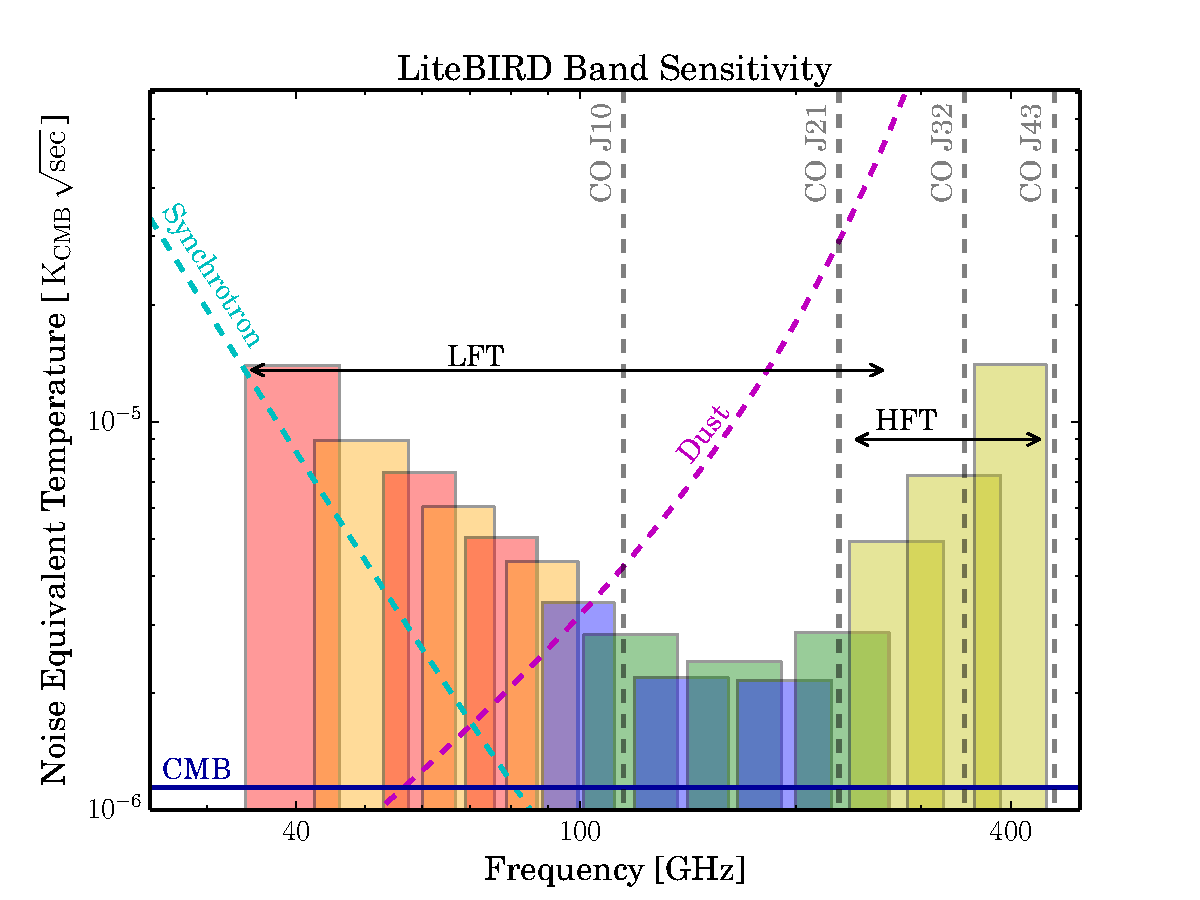
\includegraphics[width=1.1\textwidth, center]{PDF/LBSensitivity_noMargin.pdf}
	\caption{LiteBIRD sensitivity with no margin \label{fig:sens}}
\end{figure}

%%%%%%%%%%%%%%%%%%%%%%%%%%%%%%%%%%%%%

\subsection{Sensitivity With Margin}

We must add safety factors to our calculation to make them viable representations of expected instrumental performance. We add margin to the sensivity calculation using the factors presented in Table \ref{table:degFactors}. Note that the yield and observation time factors were decided prior to the LiteBIRD preproposal by Nils Halverson et al in on 2014-12-11, while the NET margin is floating and is adjusted such that we meet our $\sigma(r=0) = 5.7 \times 10^{-4}$ requirement.

\begin{table}[H]
\centering
	\begin{tabular}{|| c | c ||}
	\hline
	Parameter & Degredation Factor\\
	\hline
	\hline
	Yield & 0.8 \\
	\hline
	NET & 1.15 \\
	\hline
	Observing Time & $\mathrm{0.85 \, (cosmic \; ray) \times 0.85 \, (ADR) = 0.72}$ \\
	\hline
	\end{tabular}
\caption{LiteBIRD degredation factors \label{table:degFactors}}
\end{table}

Using the factors presented in Table \ref{table:degFactors}, we recalculate experimental sensitivity and present them in Table \ref{table:sensWithDeg} and Figure \ref{fig:sensWithDeg}.

\begin{table}[H]
\centering
	\begin{tabu}{|| c | c | c | c ||}
	\hline
	Band & Detector NET  & NET Array & Sensitivity \\
	 & $\mathrm{[\mu K\sqrt{sec}]}$ & $\mathrm{[\mu K\sqrt{sec}]}$ & $\mathrm{[\mu K - arcmin]}$ \\
	\hline
	\csvreader[head to column names, late after line= \\ \hline, late after last line=]{CSV/SensitivityWithMargin.csv}{}{\a & \b & \c & \d}
	\csvreader[head to column names, late after last line= ]{CSV/SensitivityWithMarginTotal.csv}{}{\\ \hline \multicolumn{1}{||c}{\a} & \multicolumn{1}{c}{} & \multicolumn{1}{c}{\b} & \multicolumn{1}{c ||}{\c} }
	\csvreader[head to column names, late after last line = \\ \hline]{CSV/SensitivityWithMarginCMBTotal.csv}{}{ \\ \hline \multicolumn{1}{||c}{\a} & \multicolumn{1}{c}{} & \multicolumn{1}{c}{\b} & \multicolumn{1}{c||}{\c}}
	\end{tabu}
\caption{LiteBIRD sensitivies with margin for degradation \label{table:sensWithDeg}}
\end{table}

\begin{figure}[H]
	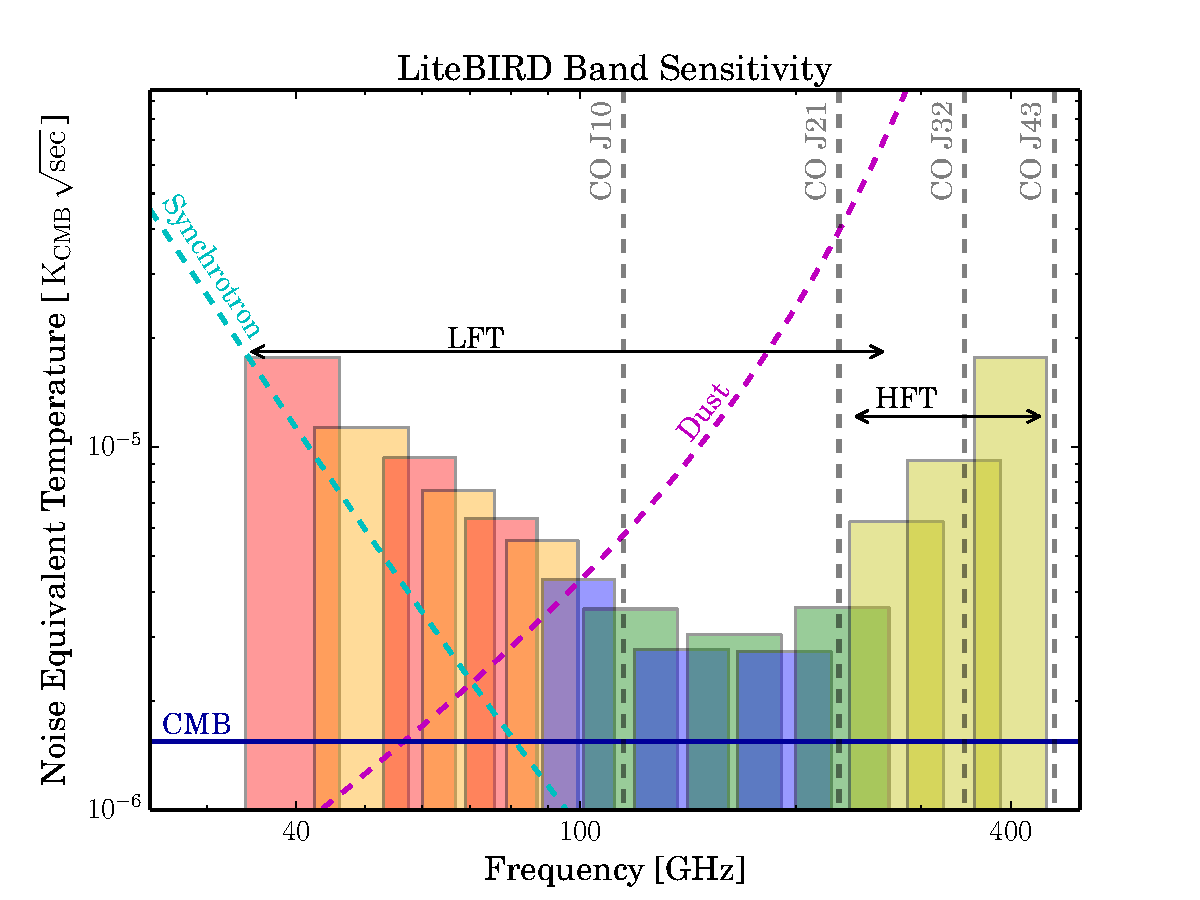
\includegraphics[width=1.1\textwidth, center]{PDF/LBSensitivity_withMargin.pdf}
	\caption{LiteBIRD sensitivity with margin \label{fig:sensWithDeg}}
\end{figure}


%%%%%%%%%%%%%%%%%%%%%%%%%%%%%%%%%%%%%%%%%%%%%%%%%%%%%%%%%%%%%%%%%%%%%%

\newpage

\section{Details of Sensitivity Calculation}

This section provides the details of the equations and techniques used to calculate our noise estimates.

%%%%%%%%%%%%%%%%%%%%%%%%%%%%%%%%%%%%% 

\subsection{Optical Power}

Optical power is calculated via

\begin{equation}
	P_{opt} = \int_{\nu_{1}}^{\nu_{2}} \; \Big[ \sum_{i = 0}^{N_{elem}}  P_{i} (T_{i}, T_{r;i}, \nu) \Big] \, \mathrm{d} \nu
	\label{eq:pOpt}
\end{equation}

where the summation runs over the optical elements from the sky towards the detector, and where $\nu_{1}$ and $\nu_{2}$ are the edges of the band in question. In Equation \ref{eq:pOpt}, I've defined 

\begin{equation}
	P_{i} (T_{i}, T_{r;i}, \nu) = E_{i} (\nu) \, S (T_{i}, \nu) + R_{i} (\nu) \, S (T_{r;i}, \nu)
	\label{eq:poptIntegrand}
\end{equation}

where $T_{i}$ is the temperature of optical element $i$, $T_{r;i}$ is the temperature that element $i$ reflects to, and $S(T, \nu)$ is the power emitted from a blackbody at temperature $T$ at frequency $\nu$ onto a diffraction-limited aperture.

\begin{equation}
	S (T, \nu) = \frac{h \, \nu}{e^{\frac{h \nu}{k_{B} \, T}} - 1}
	\label{eq:powIntegrand}
\end{equation}

In Equation \ref{eq:poptIntegrand}, I've defined 

\begin{equation}
	E_{i} = \Big[ \prod_{j = i+1}^{N_{elem}} \, \eta_{j} (\nu) \Big] \, \epsilon_{i} (\nu)
	\label{eq:effEmiss}
\end{equation}

which is the effective emissivity due to absorption: $\epsilon_{i}$ is the dielectric emissivity of element $i$, and $\Big( \prod_{j = i+1}^{N_{elem}} \, \eta_{j} \Big)$ represents the cumulative efficiency of everything detector-side of element $i$. I've also defined 

\begin{equation}
	R_{i} = \Big[ \prod_{j = i+1}^{N_{elem}} \, \eta_{j} (\nu) \Big] \, r_{i} (\nu)
	\label{eq:reflEffEmiss}
\end{equation}

which is the effective emissivity due to reflection: $r_{i}$ is the reflectivity of element $i$, and $\Big( \prod_{j = i+1}^{N_{elem}} \, \eta_{j} \Big)$ represents the cumulative efficiency of everything detector-side of element $i$.

%%%%%%%%%%%%%%%%%%%%%%%%%%%%%%%%%%%%%

\subsection{Photon NEP}

We use the following equation to calculate the photon noise equivalent power (NEP) \cite{kamThesis}

\begin{equation}
	\mathrm{NEP_{ph}} = \sqrt{\int_{\nu_{1}}^{\nu_{2}} \, [ \, 2 h \nu \sum_{i}^{N_\mathrm{elem}}  P_{i} (T_{i}, T_{r;i}, \nu) + 2 \, (\sum_{i}^{N_\mathrm{elem}}  P_{i} (T_{i}, T_{r;i}, \nu))^{2} \, ] \mathrm{d}\nu}
\end{equation}


where $P_{i}$ is defined in Equation \ref{eq:poptIntegrand}. Notice that we assume 100\% photon bunching and that we integrate over the bunching cross terms.

%%%%%%%%%%%%%%%%%%%%%%%%%%%%%%%%%%%%%

\subsection{Thermal Carrier NEP}

We use the following equation to calculate thermal carrier noise inherent to the bolometer power dissipation \cite{tokiThesis}

\begin{equation}
	\mathrm{NEP_{g}} = \sqrt{4 k_{B} P_{oper} T_{b} \frac{(n+1)^{2}}{2n + 3} \frac{(T_{c} / T_{b})^{2n + 3} - 1}{[(T_{c} / T_{b})^{n+1} - 1]^{2}}}
\end{equation}

where $T_{c} = 0.171$ K is the critical temperature, $T_{b} = 0.100$ K is the bath temperature, $n = 3$ because the thermal carrier is the phonon, and bolometer operation power is calculated as 

\begin{equation}
	P_{oper} = 2.5 \, P_{opt}
\end{equation}

%%%%%%%%%%%%%%%%%%%%%%%%%%%%%%%%%%%%%

\subsection{Readout NEP}

We mandate that the total NEP for each detector be low enough such that we can meet our $\sigma(r=0)$ requirement. Therefore, $NEP_{\mathrm{det}}$ is essentially fixed by the cosmology. To meet this requirement, we float the readout NEP, assuming that we can suppress it with more flexibility than the phton and bolometer noises. 

Hence, readout noise is calculated as 

\begin{equation}
	\mathrm{NEP_{read}} = \sqrt{\mathrm{NEP_{det}^{2} - NEP_{g}^{2} + NEP_{read}^{2}}}
\end{equation}

%%%%%%%%%%%%%%%%%%%%%%%%%%%%%%%%%%%%%

\subsection{Detector NEP}

We find the total detector noise by taking the quadrature sum of the photon, thermal, and readout NEP values

\begin{equation}
	\mathrm{NEP_{det}} = \sqrt{\mathrm{NEP_{ph}^{2} + NEP_{g}^{2} + NEP_{read}^{2}}}
\end{equation}

%%%%%%%%%%%%%%%%%%%%%%%%%%%%%%%%%%%%%

\subsection{Detector NET}

We calculate the noise equivalent temperature (NET) of a detector as \cite{kamThesis}

\begin{equation}
	\mathrm{NET_{det}} = \frac{\mathrm{NEP_{det}}}{\sqrt{2} \, (\mathrm{dP/dT_{CMB}})}
\end{equation}

where we have defined the conversion factor from power to CMB temperature units as \cite{kamThesis}

\begin{equation}
	\mathrm{dP/dT_{CMB}} = \int_{\nu_1}^{\nu_{2}} \Big[ \, \frac{\eta}{k_{B}} \Big(\frac{h \nu}{T_{CMB} (e^{h \nu / k_{B} T_{CMB}} - 1)} \Big)^{2} \, e^{h \nu / k_{B} T_{CMB}} \, \Big] \mathrm{d}{\nu}
\end{equation}

where again, $\nu_{1}$ and $\nu_{2}$ are the edges of the band. Note that the $\sqrt{2}$ enters because NEP is defined in terms of $1/\sqrt{Hz}$ and NET is defined in terms of $\sqrt{sec}$.

%%%%%%%%%%%%%%%%%%%%%%%%%%%%%%%%%%%%%

\subsection{NET Array}

NET Array is calculated as \cite{kamThesis} 

\begin{equation}
	\mathrm{NET_{arr}} = \frac{\mathrm{NET_{det}}}{\sqrt{N_{det}}}
\end{equation}

where $N_{det}$ is the number of detectors observing in the given frequency band. Note that the unit of NET Array is $\mathrm{[K\sqrt{sec}]}$

%%%%%%%%%%%%%%%%%%%%%%%%%%%%%%%%%%%%%

\subsection{Sensitivity}

Sensitivity is calculated as 

\begin{equation}
	\sigma_{S} = \sqrt{\frac{4 \pi f_{sky} \, 2 \, \mathrm{NET_{arr}}^{2}}{t_{obs}}} \Big( \frac{10800}{\pi} \Big)
\end{equation}

with $f_{sky} = 1.0$ and $t_{obs} = 3$ years $ = 94672800$ sec, as defined in Table \ref{table:LbParams}. Note that the factor of $\mathrm{\sqrt{2}}$ that accompanies $\mathrm{NET_{arr}}$ accounts for the need of two detectors to measure CMB polarization. 

The units of sensitivity are given in K-arcmin.


%%%%%%%%%%%%%%%%%%%%%%%%%%%%%%%%%%%%%%%%%%%%%%%%%%%%%%%%%%%%%%%%%%%%%%%%

\newpage

\section{Details of Optical Element Calculations \label{sec:optElemCalc}}

This section is meant to outline the considerations and assumptions behind the calculation of emissivity, reflection, and efficiency of each optical element in the optical chain of both the LFT and the HFT. 

%%%%%%%%%%%%%%%%%%%%%%%%%%%%%%%%%%%%%

\subsection{LFT HWP}

This section gives the details behind the calculation of the LFT HWP emissivity, efficiency, and scattering.

%%%%%%%%%%%%%%%%%%%

\subsubsection{Assumptions}

Table \ref{table:lftHwpAssmp} gives the assumptions for the LFT HWP.

\begin{table}[H]
	\centering
	\begin{tabularx}{\textwidth}{|| c | c | X ||}
	\hline
	Assumption & Assumed Value & Justification \\
	\hline
	\hline
	HWP Material & Sapphire, grooved AR & Discussion with Tomo on 2016-01-14 \\
	\hline
	Sapphire Thickness & $t =$ 27 mm & Discussion with Tomo on 2016-01-14. Nine 3mm plates for $\Delta \nu / \nu = 1.55$ \\
	\hline
	Sapphire Index & $n =$ 3.24 & Page 2019 of \cite{lamb}. \textcolor{red}{The average of the ordinary and extraordinary axes at 140 GHz and 300 K.} \\
	\hline
	Sapphire Loss Tangent & $\tan{\delta} = \mathrm{5 \times 10^{-5}}$ & Page 2019 of \cite{lamb} and Fig 2 of \cite{parshin} \\
	\hline
	AR Reflection & $r =$ 0.08 & Discussion with Tomo and Toki on 2016-01-14 gave 10\%, pushed to 8\% to meet sensitivity requirements \\
	\hline
	Reflection Temperature & $T_{r} =$ 5 K & 100\% of scattering goes to 5K baffling \\
	\hline
	\end{tabularx}
\caption{LFT HWP assumptions \label{table:lftHwpAssmp}}
\end{table}

%%%%%%%%%%%%%%%%%%%

\subsubsection{Emissivity}

We calculate the LFT HWP emissivity using the usual equation for absorption \cite{lamb}

\begin{equation}
	\epsilon = 1 - \mathrm{exp} (- 2 \, \pi \, t \, n \, \tan{\delta} / \lambda )
	\label{eq:lftHwpDielLoss}
\end{equation}

where the variables $t$, $n$, and $\tan{\delta}$ are defined in Table \ref{table:lftHwpAssmp}, and $\lambda$ is the wavelength of the center frequency of the band in question in vacuum. 

%%%%%%%%%%%%%%%%%%%

\subsubsection{Efficiency}

We calculate the efficiency of the LFT HWP by taking both the reflection and the absorption into account

\begin{equation}
	\eta = 1 - r - \epsilon
\end{equation}

where $\epsilon$ is defined in Equation \ref{eq:lftHwpDielLoss}, and $r$ is the reflection loss given by the value in Table \ref{table:lftHwpAssmp}.

%%%%%%%%%%%%%%%%%%%%%%%%%%%%%%%%%%%%%

\subsection{HFT HWP}

This section gives the details behind the calculation of the HFT HWP emissivity, efficiency, and scattering.

%%%%%%%%%%%%%%%%%%%

\subsubsection{Assumptions}

Table \ref{table:hftHwpAssmp} gives the assumptions for the HFT HWP.

\begin{table}[H]
	\centering
	\begin{tabularx}{\textwidth}{|| c | c | X ||}
	\hline
	Assumption & Assumed Value & Justification \\
	\hline
	\hline
	Material & Silicon, grooved AR & Discussion with Tomo on 2016-01-14 \\
	\hline
	Thickness & $t =$ 4 mm & Discussion with Tomo on 2016-01-14. Three 1.33 mm plates to give $\Delta \nu / \nu = 0.6$ \\
	\hline
	Index of Refraction & $n =$ 3.40 & Page 2020 of \cite{lamb} \\
	\hline
	Loss Tangent & $\tan{\delta} = \mathrm{5 \times 10^{-5}}$ & Page 2020 of \cite{lamb} and Fig 2 of \cite{parshin} \\
	\hline
	Reflection & $r =$ 0.02 & Achieved by Jeff McMahon using grooved silicon for $\Delta \nu / \nu = 0.6$ \\
	\hline
	Reflection Temperature & $T_{r} =$ 5 K & 100\% of scattering goes to 5K baffling \\
	\hline
	\end{tabularx}
\caption{HFT HWP assumptions \label{table:hftHwpAssmp}}
\end{table}

%%%%%%%%%%%%%%%%%%%

\subsubsection{Emissivity}

We calculate the emissivity of the HFT HWP using the usual equation for absorption \cite{lamb}

\begin{equation}
	\epsilon = 1 - \mathrm{exp} (- 2 \, \pi \, t \, n \, \tan{\delta} / \lambda )
	\label{eq:hftHwpDielLoss}
\end{equation}

where the variables $t$, $n$, and $\tan{\delta}$ are defined in Table \ref{table:hftHwpAssmp}, and $\lambda$ is the wavelength of the center frequency of the band in question in vacuum. 

%%%%%%%%%%%%%%%%%%%

\subsubsection{Efficiency}

We calculate the efficiency of the HFT HWP by taking both the reflection and the absorption into account

\begin{equation}
	\eta = 1 - r - \epsilon
\end{equation}

where $\epsilon$ is defined in Equation \ref{eq:hftHwpDielLoss}, and $r$ is the reflection loss given by the value in Table \ref{table:hftHwpAssmp}.

%%%%%%%%%%%%%%%%%%%%%%%%%%%%%%%%%%%%%

\subsection{Aperture}

This section details the calculation of the aperture emissivity and efficiency.

%%%%%%%%%%%%%%%%%%%

\subsubsection{Efficiency}

Spillover efficiency is calculated as \cite{tokiThesis}

\begin{equation}
	\eta = 1 - \mathrm{exp} \Big[ \frac{\pi^{2}}{2} \, \big( \frac{D}{w_{0} \, F \, \lambda} \big)^{2} \Big]
\end{equation}

where $F$ is the F/\# of the telescope, $D$ is the pixel diameter, $w_{0}$ is the waist ratio, and $\lambda$ is wavelength of the central frequency of the band in quesion. Values of $F$, $D$, and $w_{0}$ for the LFT are given in Table \ref{table:lftOptParams}, and the corresponding values for the HFT are given in Table \ref{table:hftOptParams}.

\begin{table}[H]
\centering
	\begin{tabularx}{\textwidth}{|| c | c | X ||}
	\hline
	\multicolumn{3}{|| c ||}{LFT Spillover Parameters} \\
	\hline
	\hline
	Opitcal Parameter & Assumed Value & Justification \\
	\hline
	\hline
	F/\# & 3.5 & Discussions with Tomo on 2016-01-12 \\
	\hline
	Beam Waist Factor $\mathrm{D/w_{0}}$ & 2.6 & Email correspondance with Tomo on 2015-01-12. Smaller than for PB2 because of many AR layers. \\
	\hline
	\end{tabularx}
\caption{LFT frequency-independent optical parameters \label{table:lftOptParams}}
\end{table}

\begin{table}[H]
\centering
	\begin{tabularx}{\textwidth}{|| c | c | X ||}
	\hline
	\multicolumn{3}{|| c ||}{HFT Spillover Parameters} \\
	\hline
	\hline
	Opitcal Parameter & Assumed Value & Justification \\
	\hline
	\hline
	F/\# & 2.2 & Guided by BICEP's refractive optical design \cite{keatingBICEP} \\
	\hline
	Beam Waist Factor $\mathrm{D/w_{0}}$ & 3.1 & Taken from an ALMA paper on corrugated horns \cite{almaCorrugatedHorn} \\
	\hline
	\end{tabularx}
\caption{HFT frequency-independent optical parameters \label{table:hftOptParams}}
\end{table}

%%%%%%%%%%%%%%%%%%%

\subsubsection{Emissivity}

Because we expect reflection from the aperture to be greatly suppressed, we take the emissivity of the aperture to be the converse of the efficiency.

\begin{equation}
	\epsilon = 1 - \eta
\end{equation}

%%%%%%%%%%%%%%%%%%%%%%%%%%%%%%%%%%%%%

\subsection{LFT Mirrors}

This section gives all of the details behind the calculation of the mirror emissivity, efficiency, and scattering.

%%%%%%%%%%%%%%%%%%%

\subsubsection{Assumptions}

Table \ref{table:mirrAssmp} lays out these assumptions behind the mirror calculations.

\begin{table}[H]
	\centering
	\begin{tabularx}{\textwidth}{|| c | c | X ||}
	\hline
	Assumption & Assumed Value & Justification \\
	\hline
	\hline
	Material & Aluminum & Discussion with Tomo and Toki on 2016-01-12 \\
	\hline
	Al Conductivity & $\sigma_{c} =$ 36.9 $\mathrm{S / \mathrm{\mu} m}$ & Wikipedia \\
	\hline
	RMS Roughness & $\sigma_{r} =$ 0.2 $\mathrm{\mu m}$ & Mirror roughness achieved by Planck \cite{planckMirror} \\
	\hline
	Reflection Temperature & $T_{r} =$ 5 K & 100\% of scattering goes to 5K baffling \\
	\hline
	\end{tabularx}
\caption{Mirror assumptions \label{table:mirrAssmp}}
\end{table}

%%%%%%%%%%%%%%%%%%%

\subsubsection{Emissivity}

To calculate the emissivity of the mirror, we take into account the ohmic loss due the finite conductivity of the metal, which is defined to be \cite{kasparek}

\begin{equation}
	\epsilon = 4 \, \sqrt{\frac{\pi \nu \mu_{0}}{\sigma_{c}}} \frac{1}{Z_{0}}
	\label{eq:ohmicLoss}
\end{equation}	

where $\nu$ is the central frequency of the band in question, $\mu_{0}$ is the permeability of free space, $Z_{0} = \sqrt{\mu_{0} / \epsilon_{0}}$ is the impedance of free space, and $\sigma_{c}$ is the reflector conductivity defined in Table \ref{table:mirrAssmp}.

%%%%%%%%%%%%%%%%%%%
\begin{comment}
\subsubsection{Reflection}

To calculate the scattering of the mirror, we take into account ineffciency due to surface roughness of the reflector, which is defined by Ruze's Equation

\begin{equation}	
	r = \mathrm{exp} \Big[ (\frac{4 \pi \sigma_{r}}{\lambda} )^{2} \Big]
	\label{eq:ruzeLoss}
\end{equation}

where $\sigma_{r}$ is the RMS surface roughness of the reflector defined in Table \ref{table:mirrAssmp} and $\lambda$ is the wavelength of the central frequency of the band in question.
\end{comment}

%%%%%%%%%%%%%%%%%%%

\subsubsection{Efficiency}

%To calculate the efficiency of the mirror, we consider both the scattering loss and the ohmic loss
\textcolor{red}{To calculate the efficiency of the mirror, we consider the ohmic loss}

\begin{equation}
	%\eta = 1 - \epsilon- r
	\textcolor{red}{\eta = 1 	- \epsilon}
\end{equation}

%where $\epsilon$ is defined in Equation \ref{eq:ohmicLoss} and $r$ is defined in Equation \ref{eq:ruzeLoss}.
\textcolor{red}{where $\epsilon$ is defined in Equation \ref{eq:ohmicLoss}.} 

%%%%%%%%%%%%%%%%%%%%%%%%%%%%%%%%%%%%%

\subsection{HFT Lenses}

This section gives the details behind the calculation of the HFT lens emissivity, efficiency, and scattering.

%%%%%%%%%%%%%%%%%%%

\subsubsection{Assumptions}

Table \ref{table:hftLensAssmp} lays out the assumptions behind the HFT Lens calculations.

\begin{table}[H]
	\centering
	\begin{tabularx}{\textwidth}{|| c | c | X ||}
	\hline
	Assumption & Assumed Value & Justification \\
	\hline
	\hline
	Lens Material & Silicon, grooved AR & Discussion with Tomo 2016-01-12 \\
	\hline
	Thickness & $t =$ 20 mm & Discussion with Tomo 2016-01-14: minimum rigidity needed for safe launch (rough guess) \\
	\hline
	Silicon Index & $n =$ 3.40 & Page 2020 of \cite{lamb} \\
	\hline
	Silicon Loss Tangent & $\tan{\delta} = \mathrm{5 \times 10^{-5}}$ & Page 2020 of \cite{lamb} and Fig 2 of \cite{parshin} \\
	\hline
	AR Reflection & $r =$ 0.02 & Achieved by Jeff McMahon using grooved silicon for $\Delta \nu / \nu = 0.6$ \\
	\hline
	Reflection Temperature & $T_{r} =$ 5 K & 100\% of scattering goes to 5K baffling \\
	\hline
	\end{tabularx}
\caption{HFT Lens assumptions \label{table:hftLensAssmp}}
\end{table}

%%%%%%%%%%%%%%%%%%%

\subsubsection{Emissivity}

We calculate the emissivity of the HFT lenses using the usual equation for absorption

\begin{equation}
	\epsilon = 1 - \mathrm{exp} (- 2 \, \pi \, t \, n \, \tan{\delta} / \lambda )
	\label{eq:hftLensDielLoss}
\end{equation}

where the variables $t$, $n$, and $\tan{\delta}$ are defined in Table \ref{table:hftHwpAssmp}, and $\lambda$ is the wavelength of the center frequency of the band in question.

%%%%%%%%%%%%%%%%%%%

\subsubsection{Efficiency}

We calculate the efficiency of the HFT lens by taking both the reflection and the absorption into account

\begin{equation}
	\eta = 1 - r - \epsilon
\end{equation}

where $\epsilon$ is defined in Equation \ref{eq:hftLensDielLoss}, and $r$ is the reflection loss given by the value in Table \ref{table:hftLensAssmp}.

%%%%%%%%%%%%%%%%%%%%%%%%%%%%%%%%%%%%%

\subsection{2 K Filter}

This section gives the details behind the calculation of the LFT and HFT 2 K filter emissivity, efficiency, and scattering.

%%%%%%%%%%%%%%%%%%%

\subsubsection{Assumptions}

Table \ref{table:2kfAssmp} lays out these assumptions behind the 2 K Filter calculations.

\begin{table}[H]
	\centering
	\begin{tabularx}{\textwidth}{|| c | c | X ||}
	\hline
	Assumption & Assumed Value & Justification \\
	\hline
	\hline
	Substrate Material & Polypropylene & Cardiff filter design \cite{cardiff} \\
	\hline
	Substrate Thickness & $t =$ 5 mm & Discussion with Tomo 2016-01-12: measuring a spare filter in the UCB lab \\
	\hline
	Substrate Index & $n =$ 1.5 & Page 2013 of \cite{lamb} \\
	\hline
	Loss Tangent & $\tan{\delta} = \mathrm{2.3 \times 10^{-4}}$ & Page 2013 of \cite{lamb} \\
	\hline
	AR Reflection & $r =$ 0.05 & Discussion with Tomo on 2016-01-14, looking at a plot from \cite{bolowikiMMF} \\
	\hline
	Reflection Temperature & $T_{r} =$ 100 mK & 100\% of scattering goes to back to focal plane \\
	\hline
	\end{tabularx}
\caption{2 K Filter assumptions \label{table:2kfAssmp}}
\end{table}

%%%%%%%%%%%%%%%%%%% 

\subsubsection{Emissivity}

We calculate the emissivity of the HFT lenses using the usual equation for absorption

\begin{equation}
	\epsilon = 1 - \mathrm{exp} (- 2 \, \pi \, t \, n \, \tan{\delta} / \lambda )
	\label{eq:2kfDielLoss}
\end{equation}

where the variables $t$, $n$, and $\tan{\delta}$ are defined in Table \ref{table:2kfAssmp}, and $\lambda$ is the wavelength of the center frequency of the band in question.

%%%%%%%%%%%%%%%%%%%

\subsubsection{Efficiency}

We calculate the efficiency of the HFT lens by taking both the reflection and the absorption into account

\begin{equation}
	\eta = 1 - r - \epsilon
\end{equation}

where $\epsilon$ is defined in Equation \ref{eq:2kfDielLoss}, and $r$ is the reflection loss given by the value in Table \ref{table:2kfAssmp}.

%%%%%%%%%%%%%%%%%%%%%%%%%%%%%%%%%%%%%

\subsection{LFT Lenslet}

This section gives the details behind the calculation of the LFT Lenslet emissivity, efficiency, and scattering.

%%%%%%%%%%%%%%%%%%%

\subsubsection{Assumptions}

Table \ref{table:lftLensletAssmp} lays out these assumptions behind the LFT Lenslet calculations.

\begin{table}[H]
	\centering
	\begin{tabularx}{\textwidth}{|| c | c | X ||}
	\hline
	Assumption & Assumed Value & Justification \\
	\hline
	\hline
	Lenlet Material & Silicon, grooved AR & Discussion with Toki on 2016-01-12 \\
	\hline
	Lenlset Thickness & $t =$ 9 mm & Estimated average thickness using LFT pixel radii \\
	\hline
	Silicon Index & $n =$ 3.4 & Page 2020 of \cite{lamb} \\
	\hline
	Silicon Loss Tangent & $\tan{\delta} = \mathrm{5 \times 10^{-5}}$ & Page 2020 of \cite{lamb} and Fig 2 of \cite{parshin} \\
	\hline
	AR Reflection & $r =$ 0.05 & Discussion with Toki and Tomo on 2016-01-15 \\
	\hline
	Reflection Temperature & $T_{r} =$ 100 mK & 100\% of scattering goes to back to focal plane \\
	\hline
	\end{tabularx}
\caption{LFT Lenslet assumptions \label{table:lftLensletAssmp}}
\end{table}

%%%%%%%%%%%%%%%%%%%

\subsubsection{Emissivity}

We calculate the emissivity of the LFT Lenslet using the usual equation for absorption

\begin{equation}
	\epsilon = 1 - \mathrm{exp} (- 2 \, \pi \, t \, n \, \tan{\delta} / \lambda )
	\label{eq:lftLensletDielLoss}
\end{equation}

where the variables $t$, $n$, and $\tan{\delta}$ are defined in Table \ref{table:lftLensletAssmp}, and $\lambda$ is the wavelength of the center frequency of the band in question.

%%%%%%%%%%%%%%%%%%%

\subsubsection{Efficiency}

We calculate the efficiency of the HFT lens by taking both the reflection and the absorption into account

\begin{equation}
	\eta = 1 - r - \epsilon
\end{equation}

where $\epsilon$ is defined in Equation \ref{eq:lftLensletDielLoss}, and $r$ is the reflection loss given by the value in Table \ref{table:lftLensletAssmp}.

%%%%%%%%%%%%%%%%%%%%%%%%%%%%%%%%%%%%%

\subsection{LFT Detector}

This section gives the details behind the calculation of the LFT Detector efficiency.

%%%%%%%%%%%%%%%%%%%

\subsubsection{Assumptions}

Table \ref{table:lftDetAssmp} lays out these assumptions behind LFT Detector calculations.

\begin{table}[H]
	\centering
	\begin{tabularx}{\textwidth}{|| c | c | X ||}
	\hline
	Assumption & Assumed Value & Justification \\
	\hline
	\hline
	Reflection/Absorption & $\epsilon =$ 0.32 & 30\% estimate from Toki on 2016-01-12, plus an additional 98\% optical coupling factor \\
	\hline
	\end{tabularx}
\caption{LFT Detector assumptions \label{table:lftDetAssmp}}
\end{table}

%%%%%%%%%%%%%%%%%%%

\subsubsection{Efficiency}

We calculate the efficiency of the LFT Detector by taking the converse of the absorption in the on-chip transimssion line

\begin{equation}
	\eta = 1 - \epsilon
\end{equation}

where $\epsilon$ is the absorption loss given by the value in Table \ref{table:lftDetAssmp}.

%%%%%%%%%%%%%%%%%%%%%%%%%%%%%%%%%%%%%

\subsection{HFT Detector}

This section gives the details behind the calculation of the HFT Detector efficiency.

%%%%%%%%%%%%%%%%%%%

\subsubsection{Assumptions}

 Table \ref{table:hftDetAssmp} lays out these assumptions behind the HFT Detector calculations.

\begin{table}[H]
	\centering
	\begin{tabularx}{\textwidth}{|| c | c | X ||}
	\hline
	Assumption & Assumed Value & Justification \\
	\hline
	\hline
	Reflection/Absorption & $\epsilon =$ 0.34 & 30\% conservative estimate from Hannes via email on 2016-01-13, with an additional 96\% optical coupling factor \\
	\hline
	\end{tabularx}
\caption{HFT Detector assumptions \label{table:hftDetAssmp}}
\end{table}

%%%%%%%%%%%%%%%%%%%

\subsubsection{Efficiency}

We calculate the efficiency of the HFT Detector by taking the converse of the absorption in the on-chip OMT

\begin{equation}
	\eta = 1 - \epsilon
\end{equation}

where $\epsilon$ is the absorption loss given by the value in Table \ref{table:hftDetAssmp}.


%%%%%%%%%%%%%%%%%%%%%%%%%%%%%%%%%%%%%%%%%%%%%%%%%%%%%%%%%%%%%%%%%%%%%%

\newpage

\section{Pixel Diameter Optimization \label{sec:pixOpt}}

We optimize the pixel diamter of both telescopes by maximizing mapping speed for each pixel. Mapping speed is calculated using the following equation \cite{kamThesis}

\begin{equation}
	\mathrm{MS} \propto \frac{1}{\mathrm{NET_{det}}^{2}} \; \; \; [\mathrm{K^{-2} \, sec^{-1}} ]
\end{equation}

To thorougly asses all possible scenarios, we will optimize pixel diameter for the following situations:
\begin{itemize}
	\item Fixed Field of View (FOV) vs Fixed Detector Number
	\item All reflections go to baffling vs all reflections go back to the focal plane
	\item Observation of an extended source vs of a point source
\end{itemize}

Note that this is not a calculation of pixel spacing, which is determined by number of detectors, the geometry of the wafer, and the fraction of the wafer area that can be occupied by blometers and antennas.

For this section, we will use the naming convention outlined in Table \ref{table:lftPixNaming} to differentiate pixels on the LFT

\begin{table}[H]
\centering
	\begin{tabu}{|| c | c ||}
	\hline
	LFT Pixel & LFT Detectors \\
	\hline
	\hline
	LF-135 & LF-1, LF-3, LF-5 \\
	\hline
	LF-246 & LF-2, LF-4, LF-6 \\
	\hline
	MF-135 & MF-1, MF-3, MF-5 \\	
	\hline
	MF-246 & MF-2, MF-4, MF-6 \\
	\hline
	\end{tabu}
\caption{LFT Pixel naming convention \label{table:lftPixNaming}}
\end{table}

%%%%%%%%%%%%%%%%%%%%%%%%%%%%%%%%%%%%%

\subsection{Reflections Go to Baffle, Fixed FOV}

This subsection containts the results for the optimization of pixel diameters for the LFT and HFT given a fixed field of view and assuming all reflections go to the baffling.

\clearpage

%%%%%%%%%%%%%%%%%%%

\subsubsection{LF-135}

\begin{figure}[H]
	\centering
	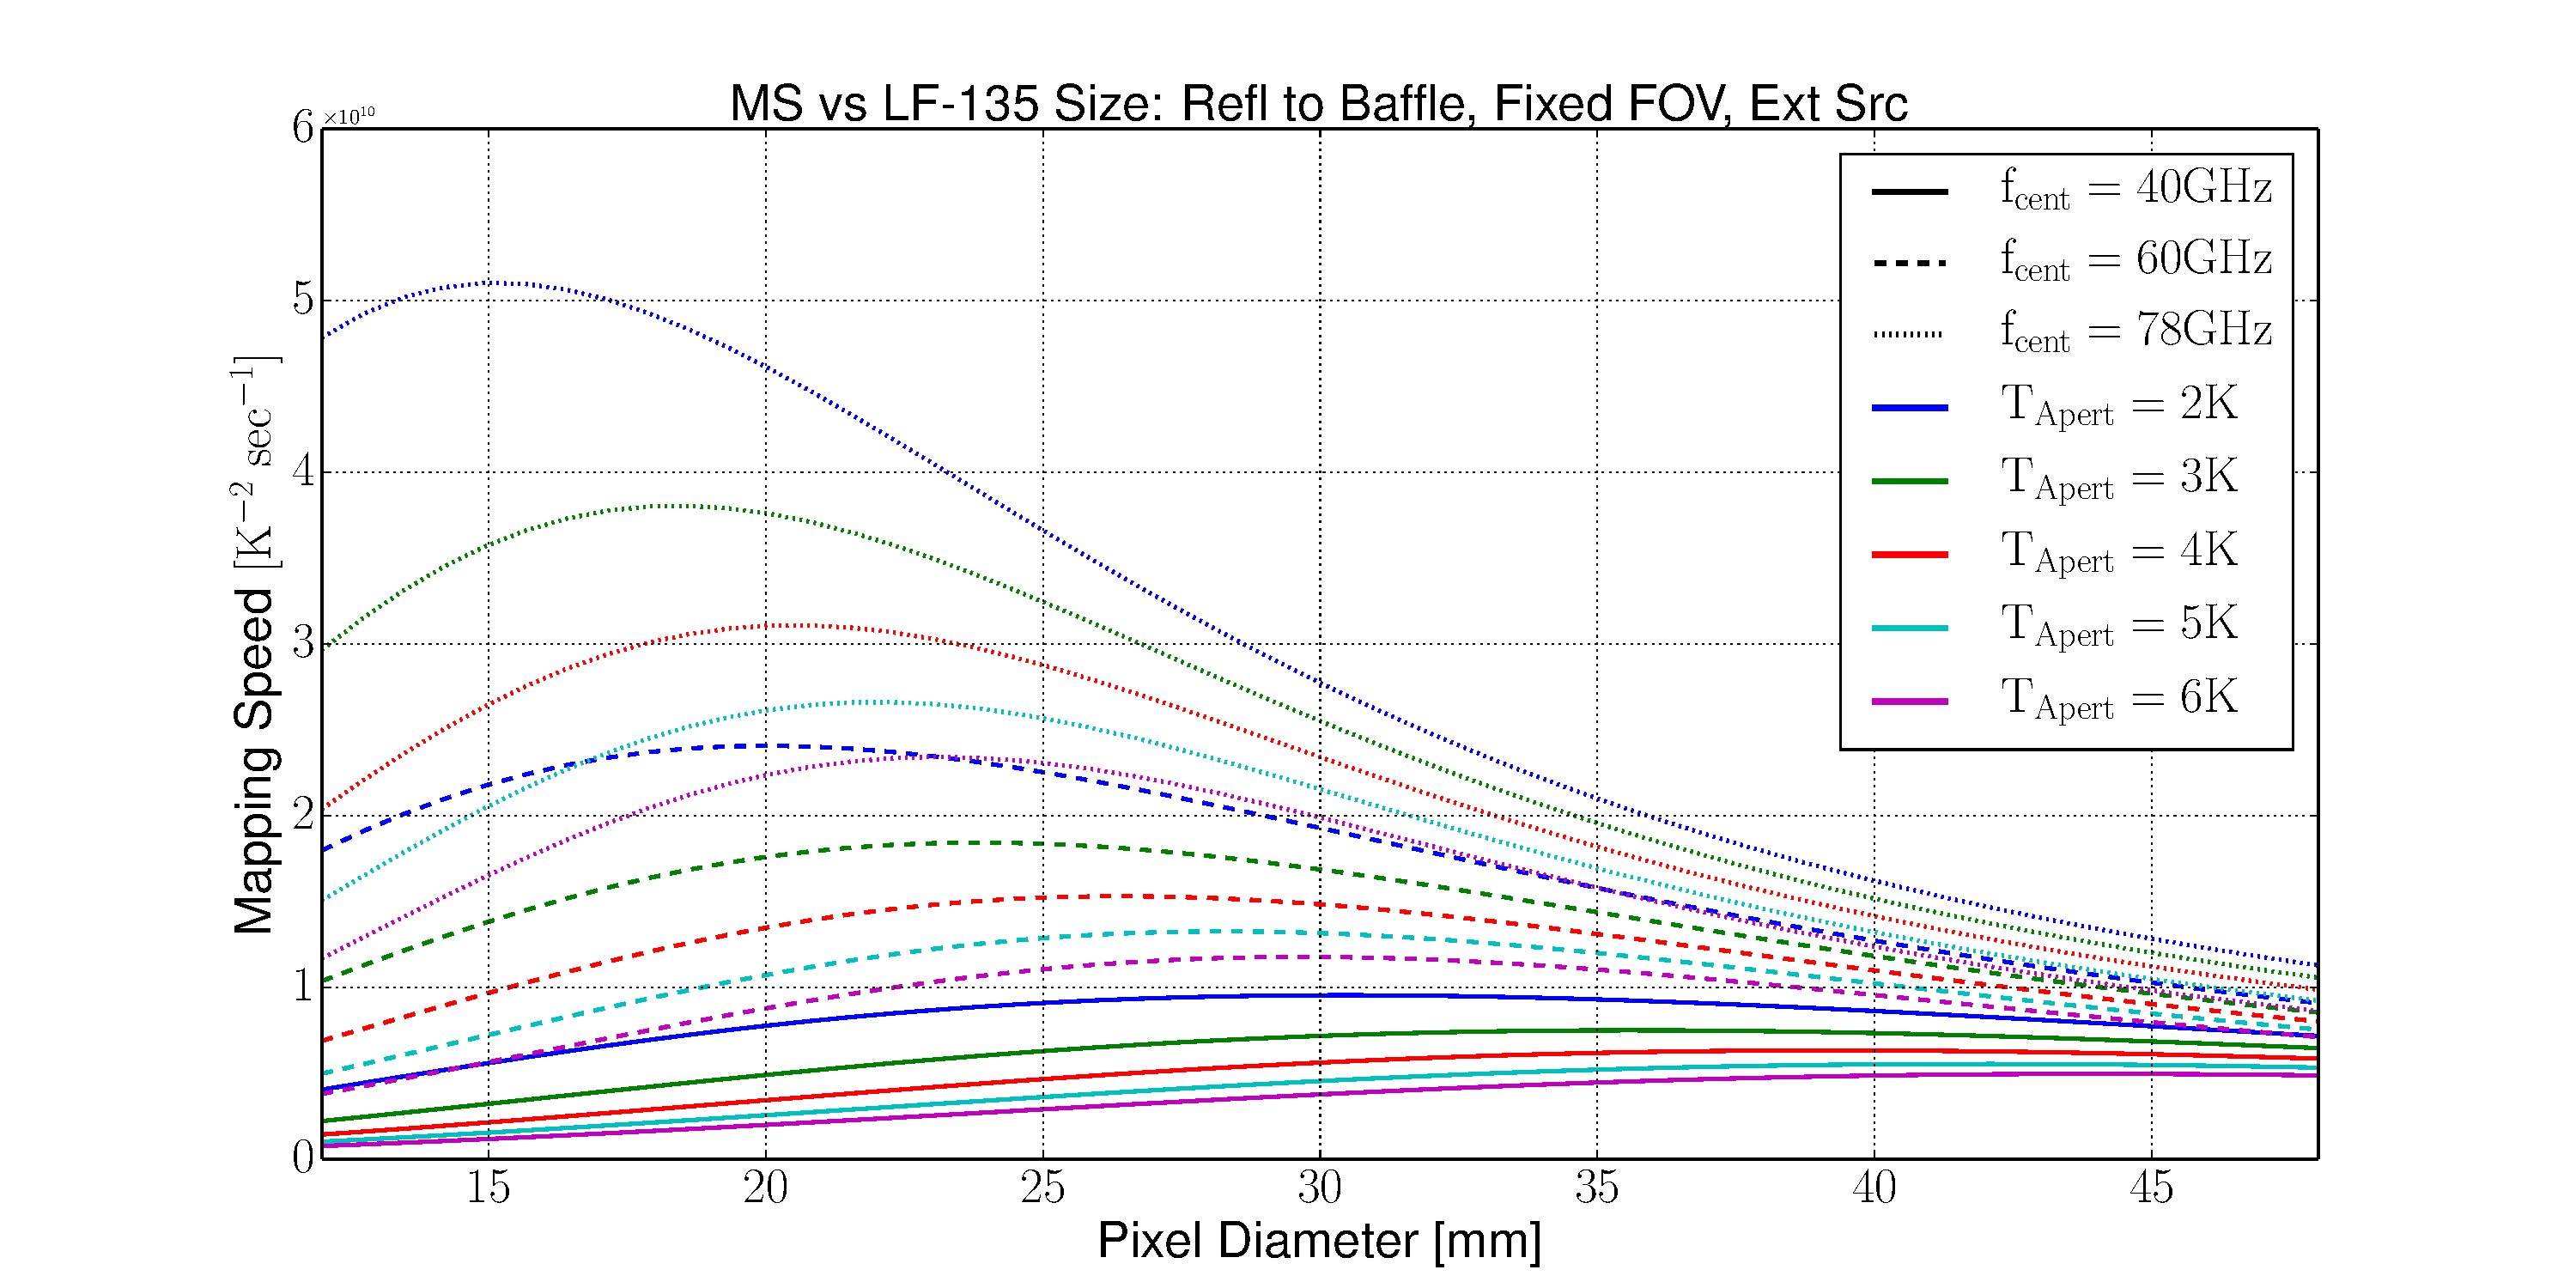
\includegraphics[width=1.1\textwidth, center]{PDF/LFT_MS_LF-135_hotRefl_fixFOV_extSrc.pdf}
	\caption{LF-135 mapping speed of an extended source as a function of pixel diameter for hot reflections and fixed FOV}
\end{figure}

\begin{figure}[H]
	\centering
	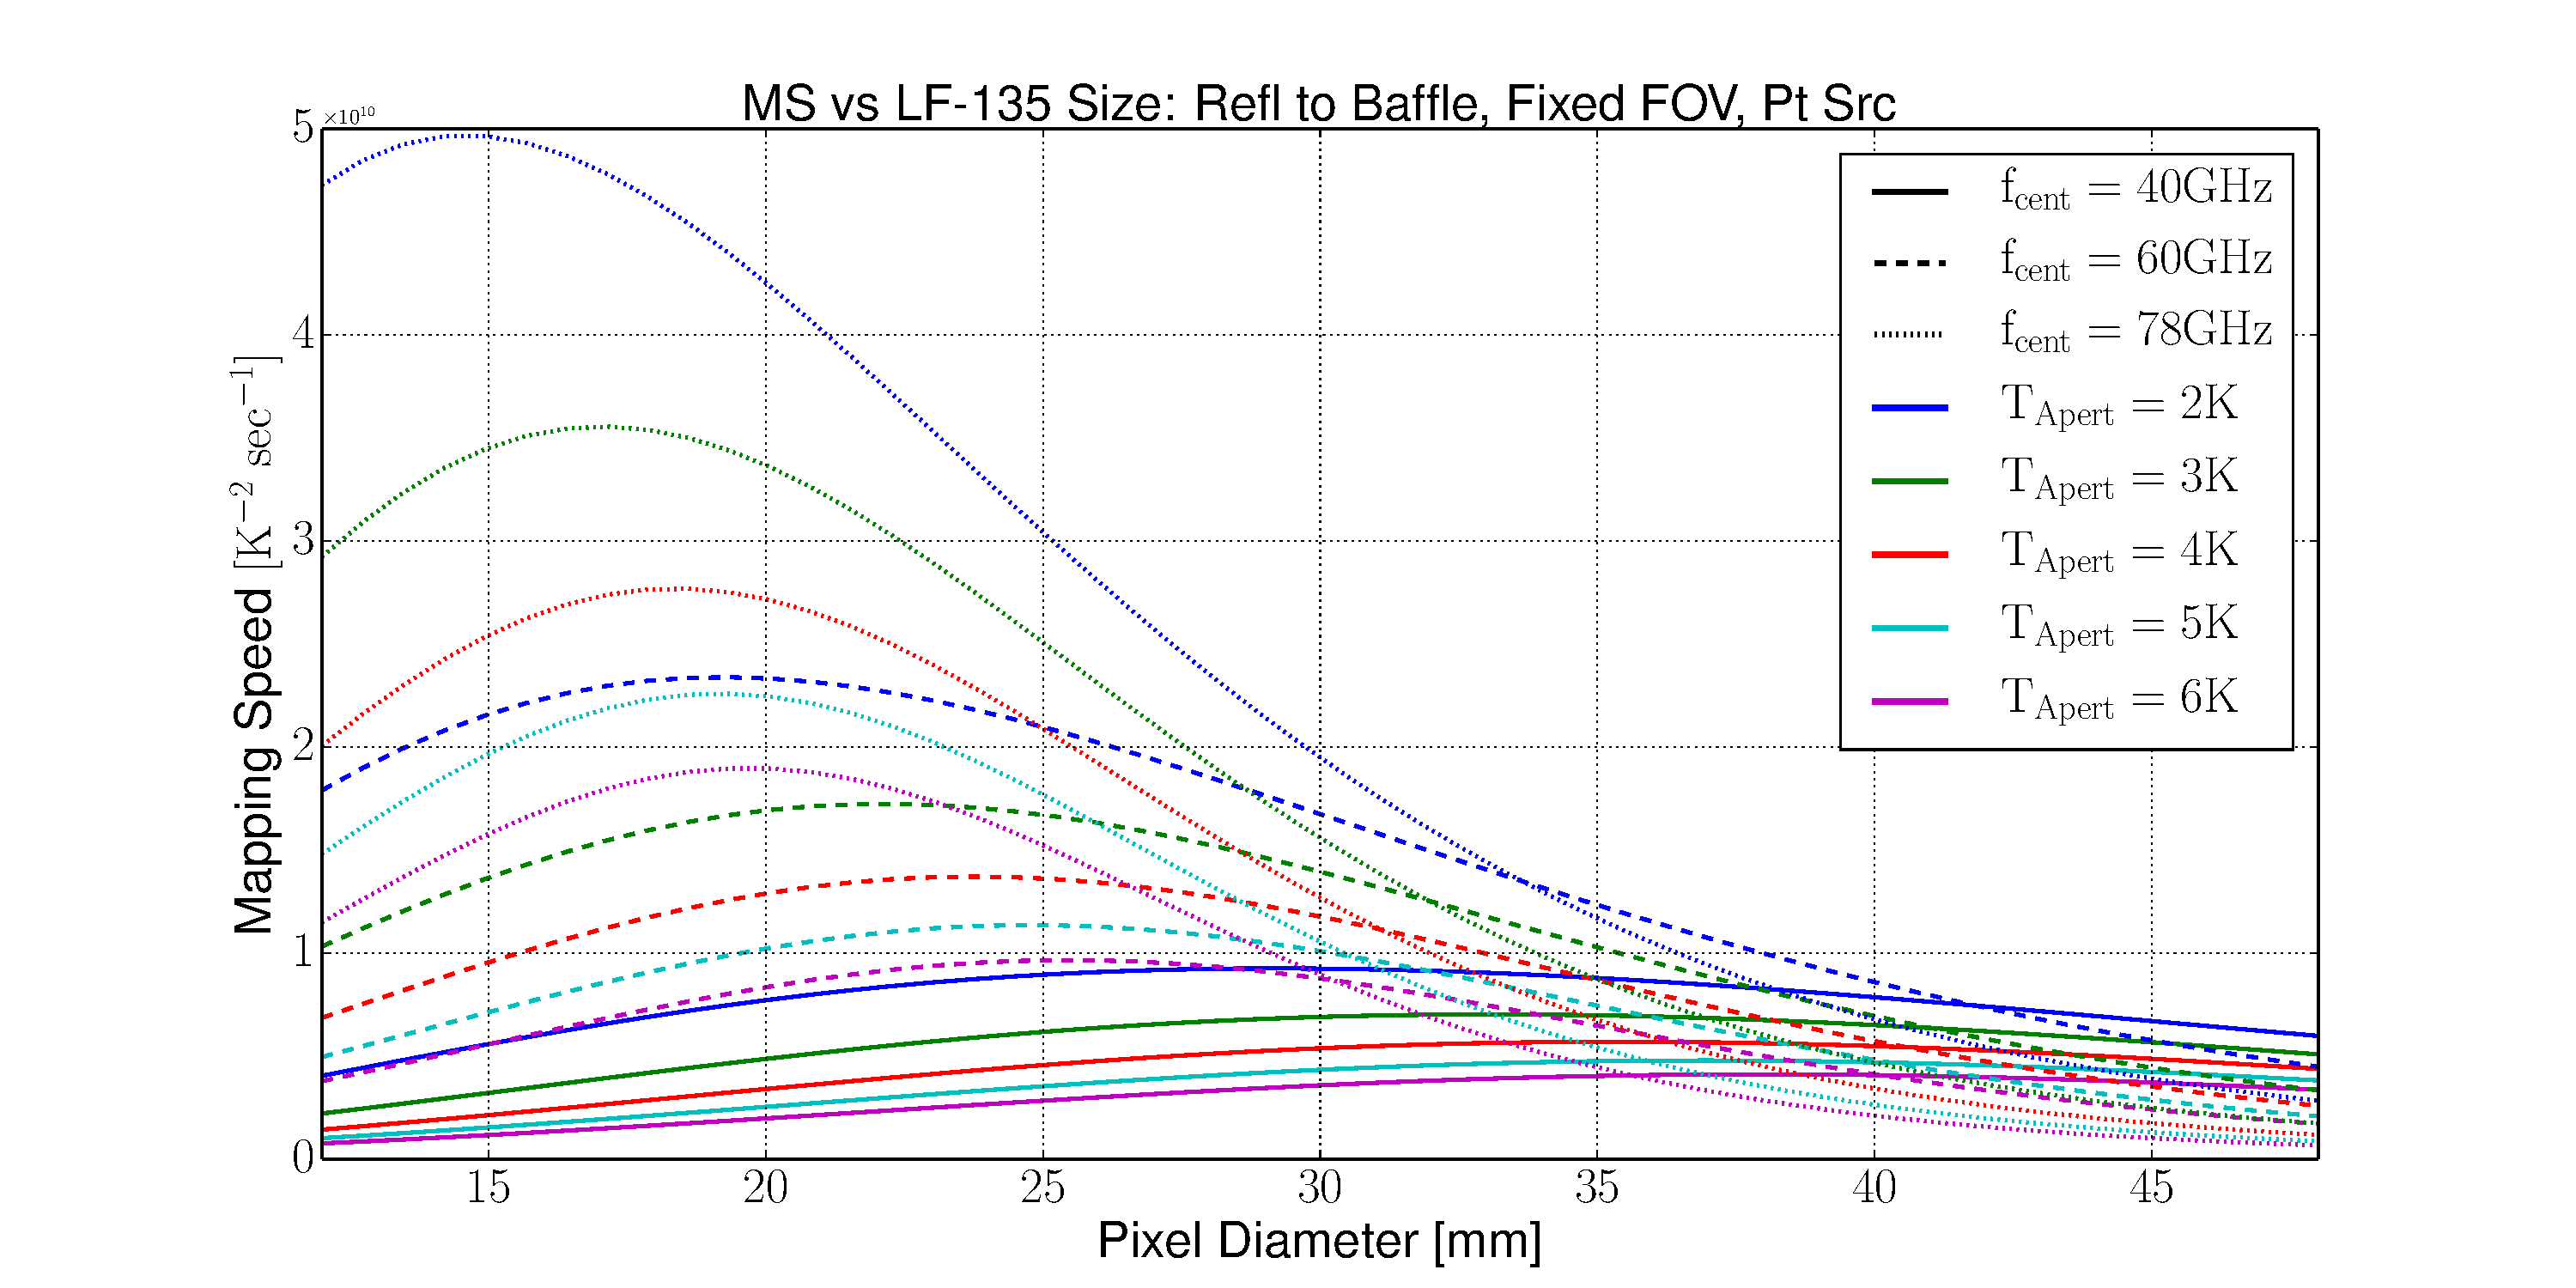
\includegraphics[width=1.1\textwidth, center]{PDF/LFT_MS_LF-135_hotRefl_fixFOV_ptSrc.pdf}
	\caption{LF-135 mapping speed of a point source as a function of pixel diameter for hot reflections and fixed FOV}
\end{figure}

%%%%%%%%%%%%%%%%%%%

\subsubsection{LF-246}

\begin{figure}[H]
	\centering
	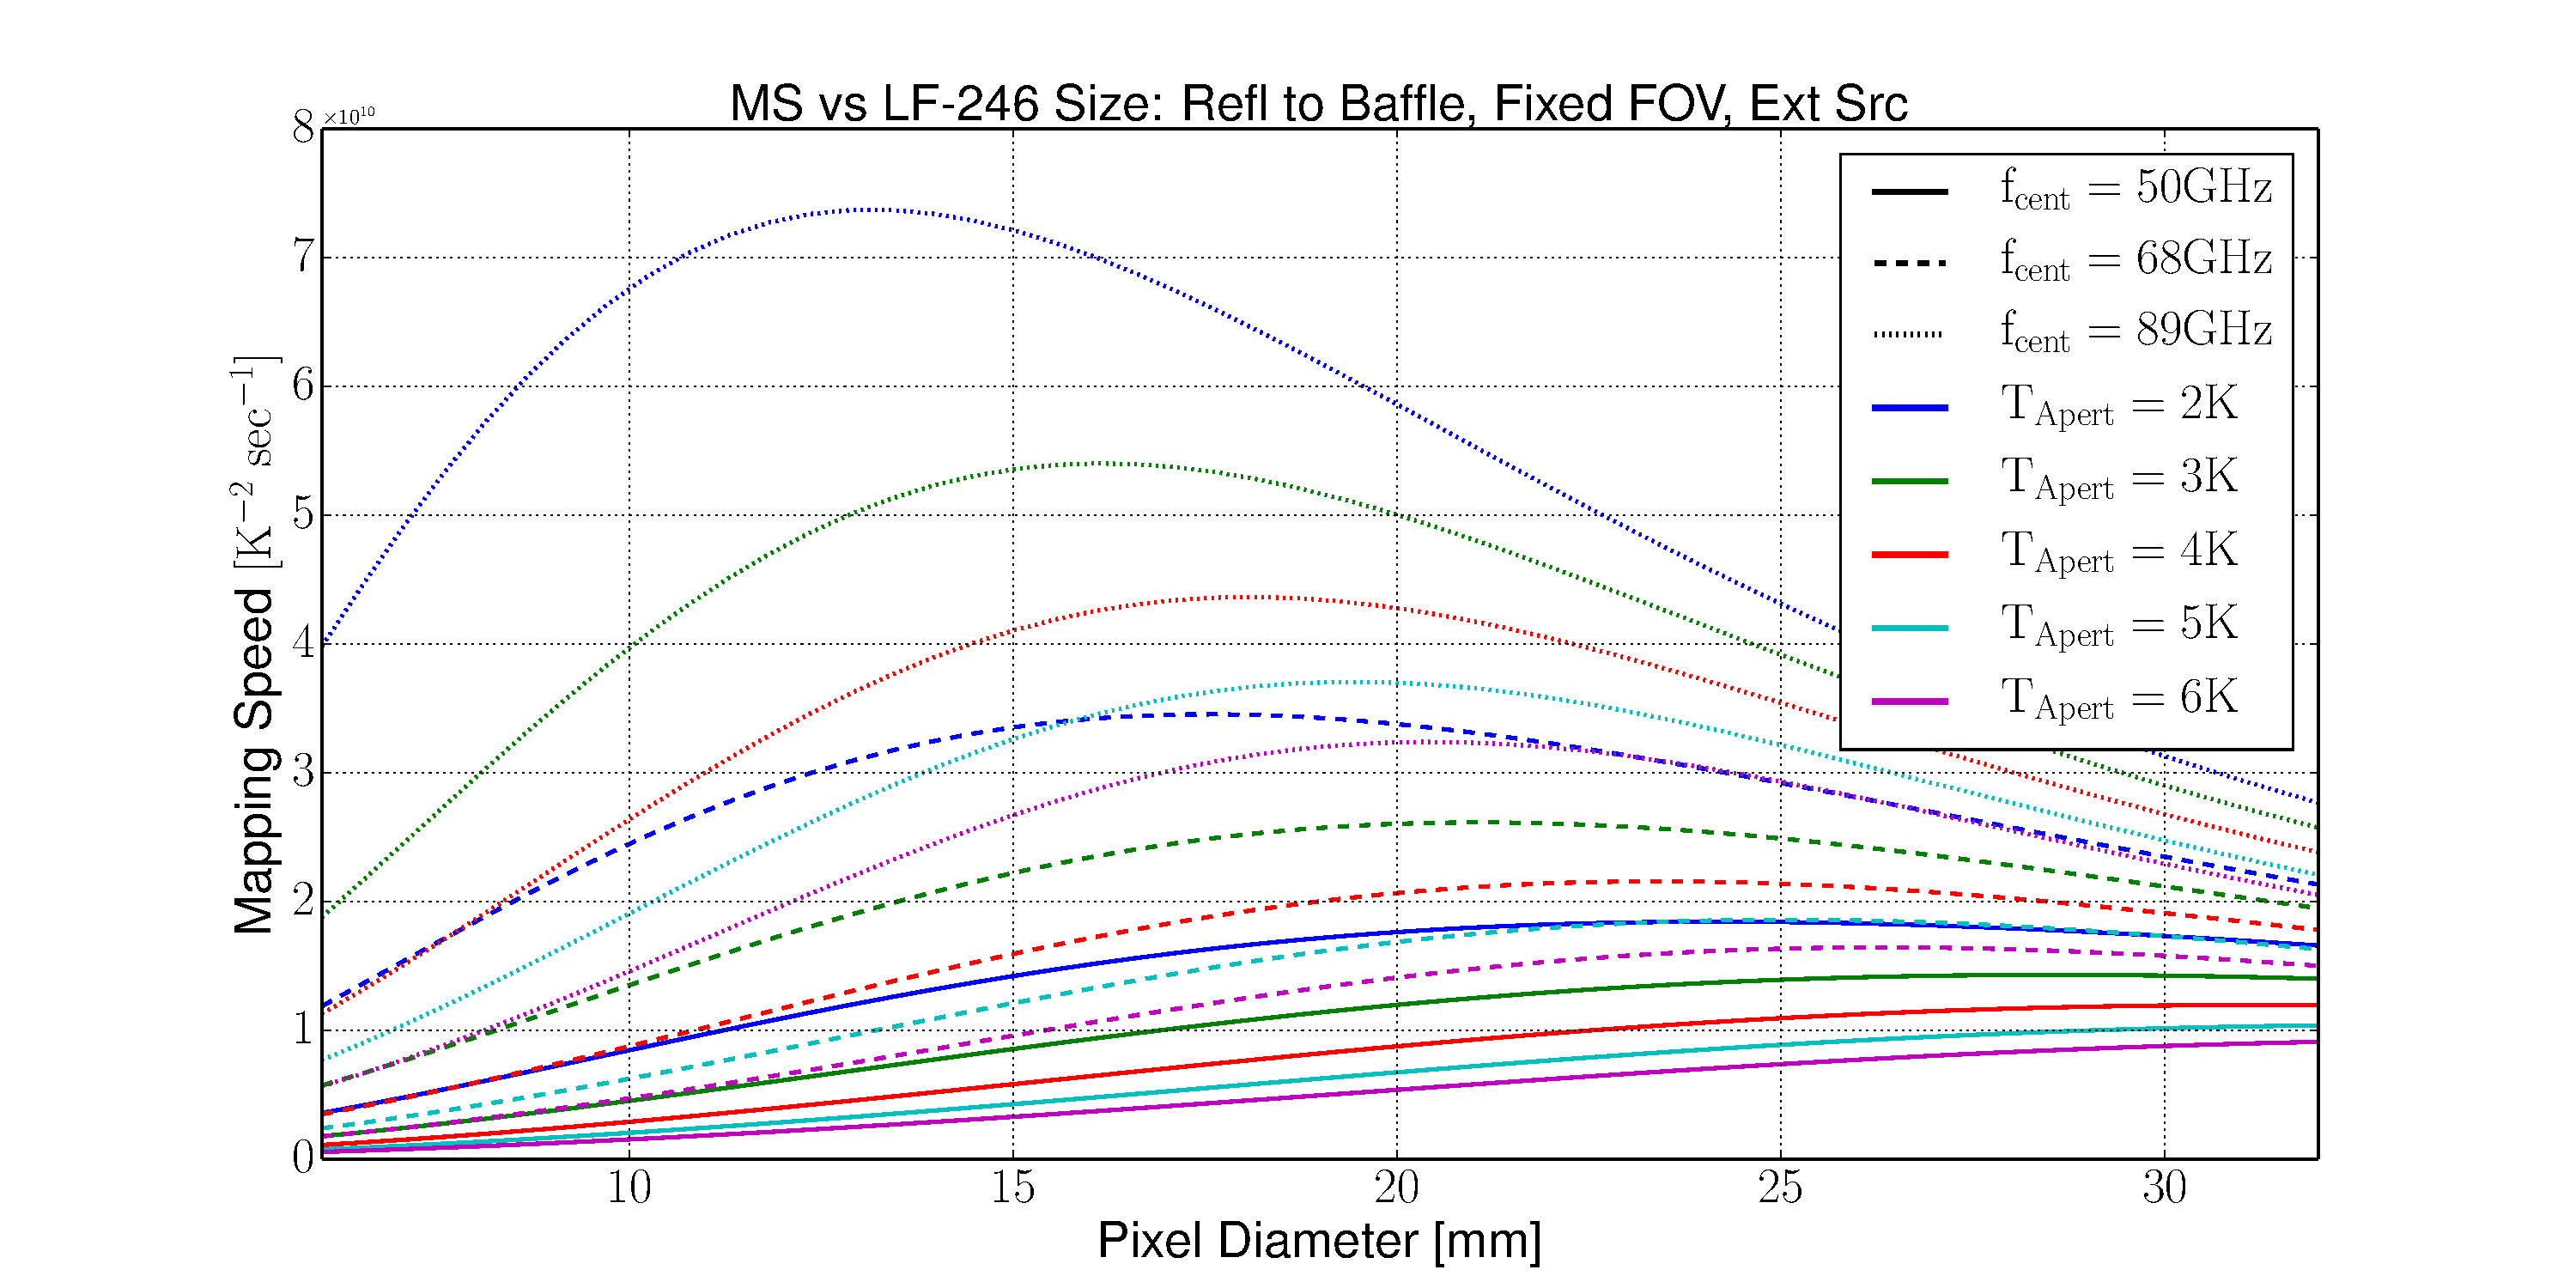
\includegraphics[width=1.1\textwidth, center]{PDF/LFT_MS_LF-246_hotRefl_fixFOV_extSrc.pdf}
	\caption{LF-246 mapping speed of an extended source as a function of pixel diameter for hot reflections and fixed FOV}
\end{figure}

\begin{figure}[H]
	\centering
	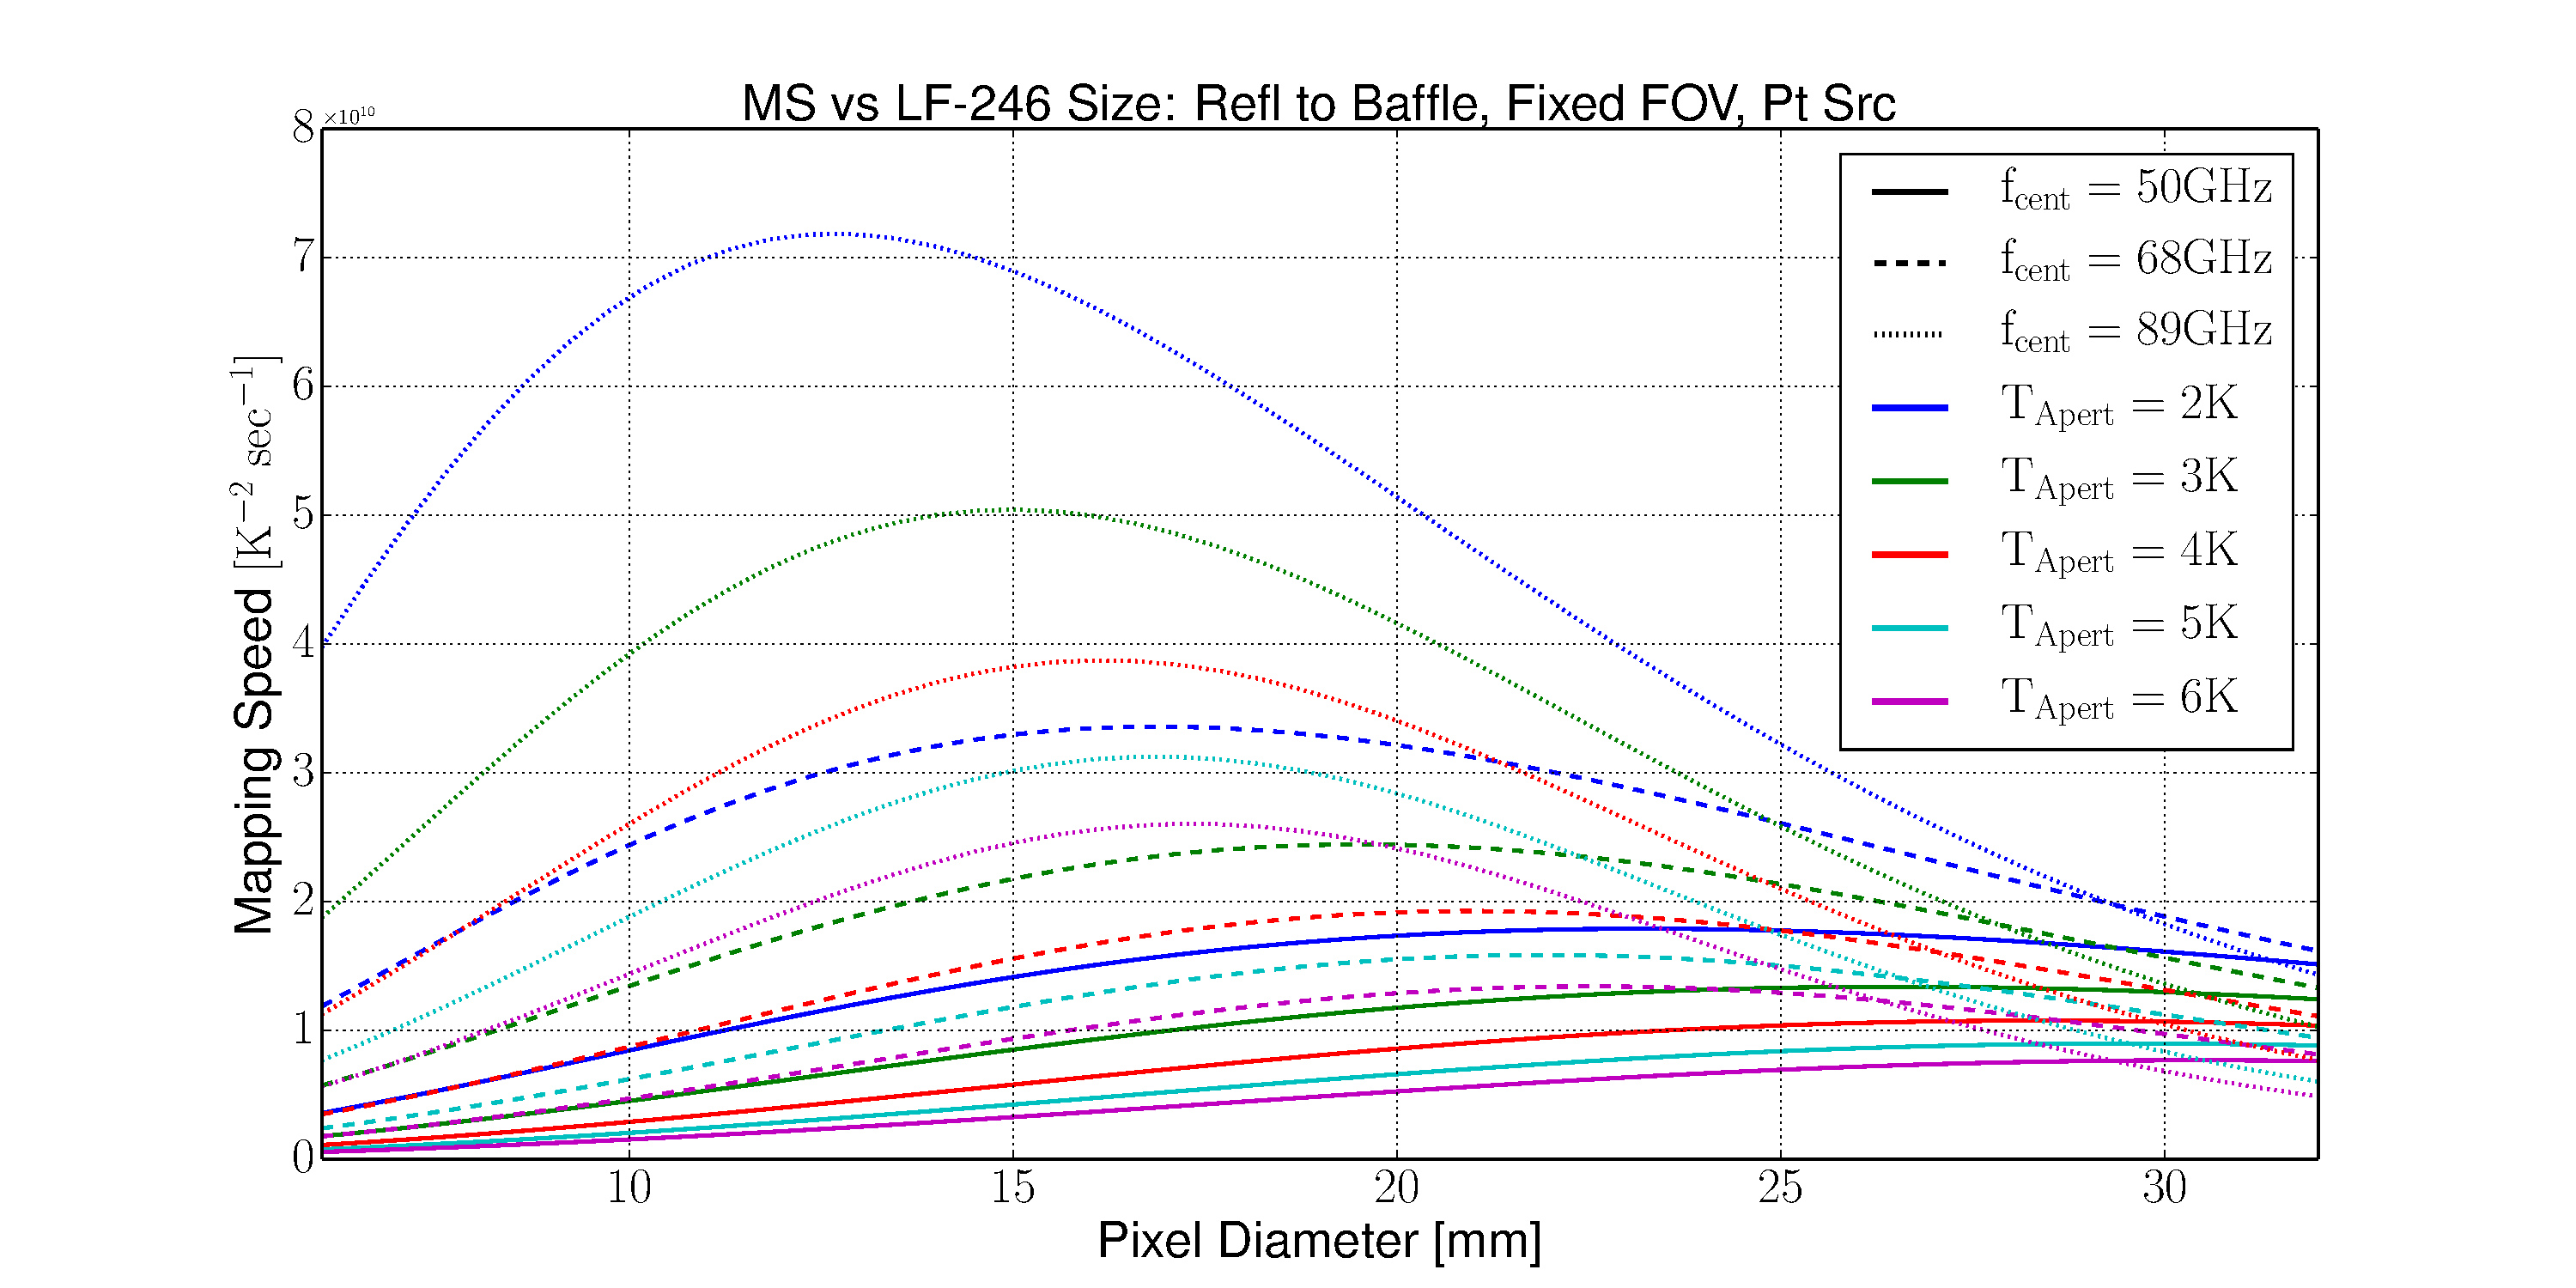
\includegraphics[width=1.1\textwidth, center]{PDF/LFT_MS_LF-246_hotRefl_fixFOV_ptSrc.pdf}
	\caption{LF-246 mapping speed of a point source as a function of pixel diameter for hot reflections and fixed FOV}
\end{figure}

%%%%%%%%%%%%%%%%%%%

\subsubsection{MF-135 Pixel}

\begin{figure}[H]
	\centering
	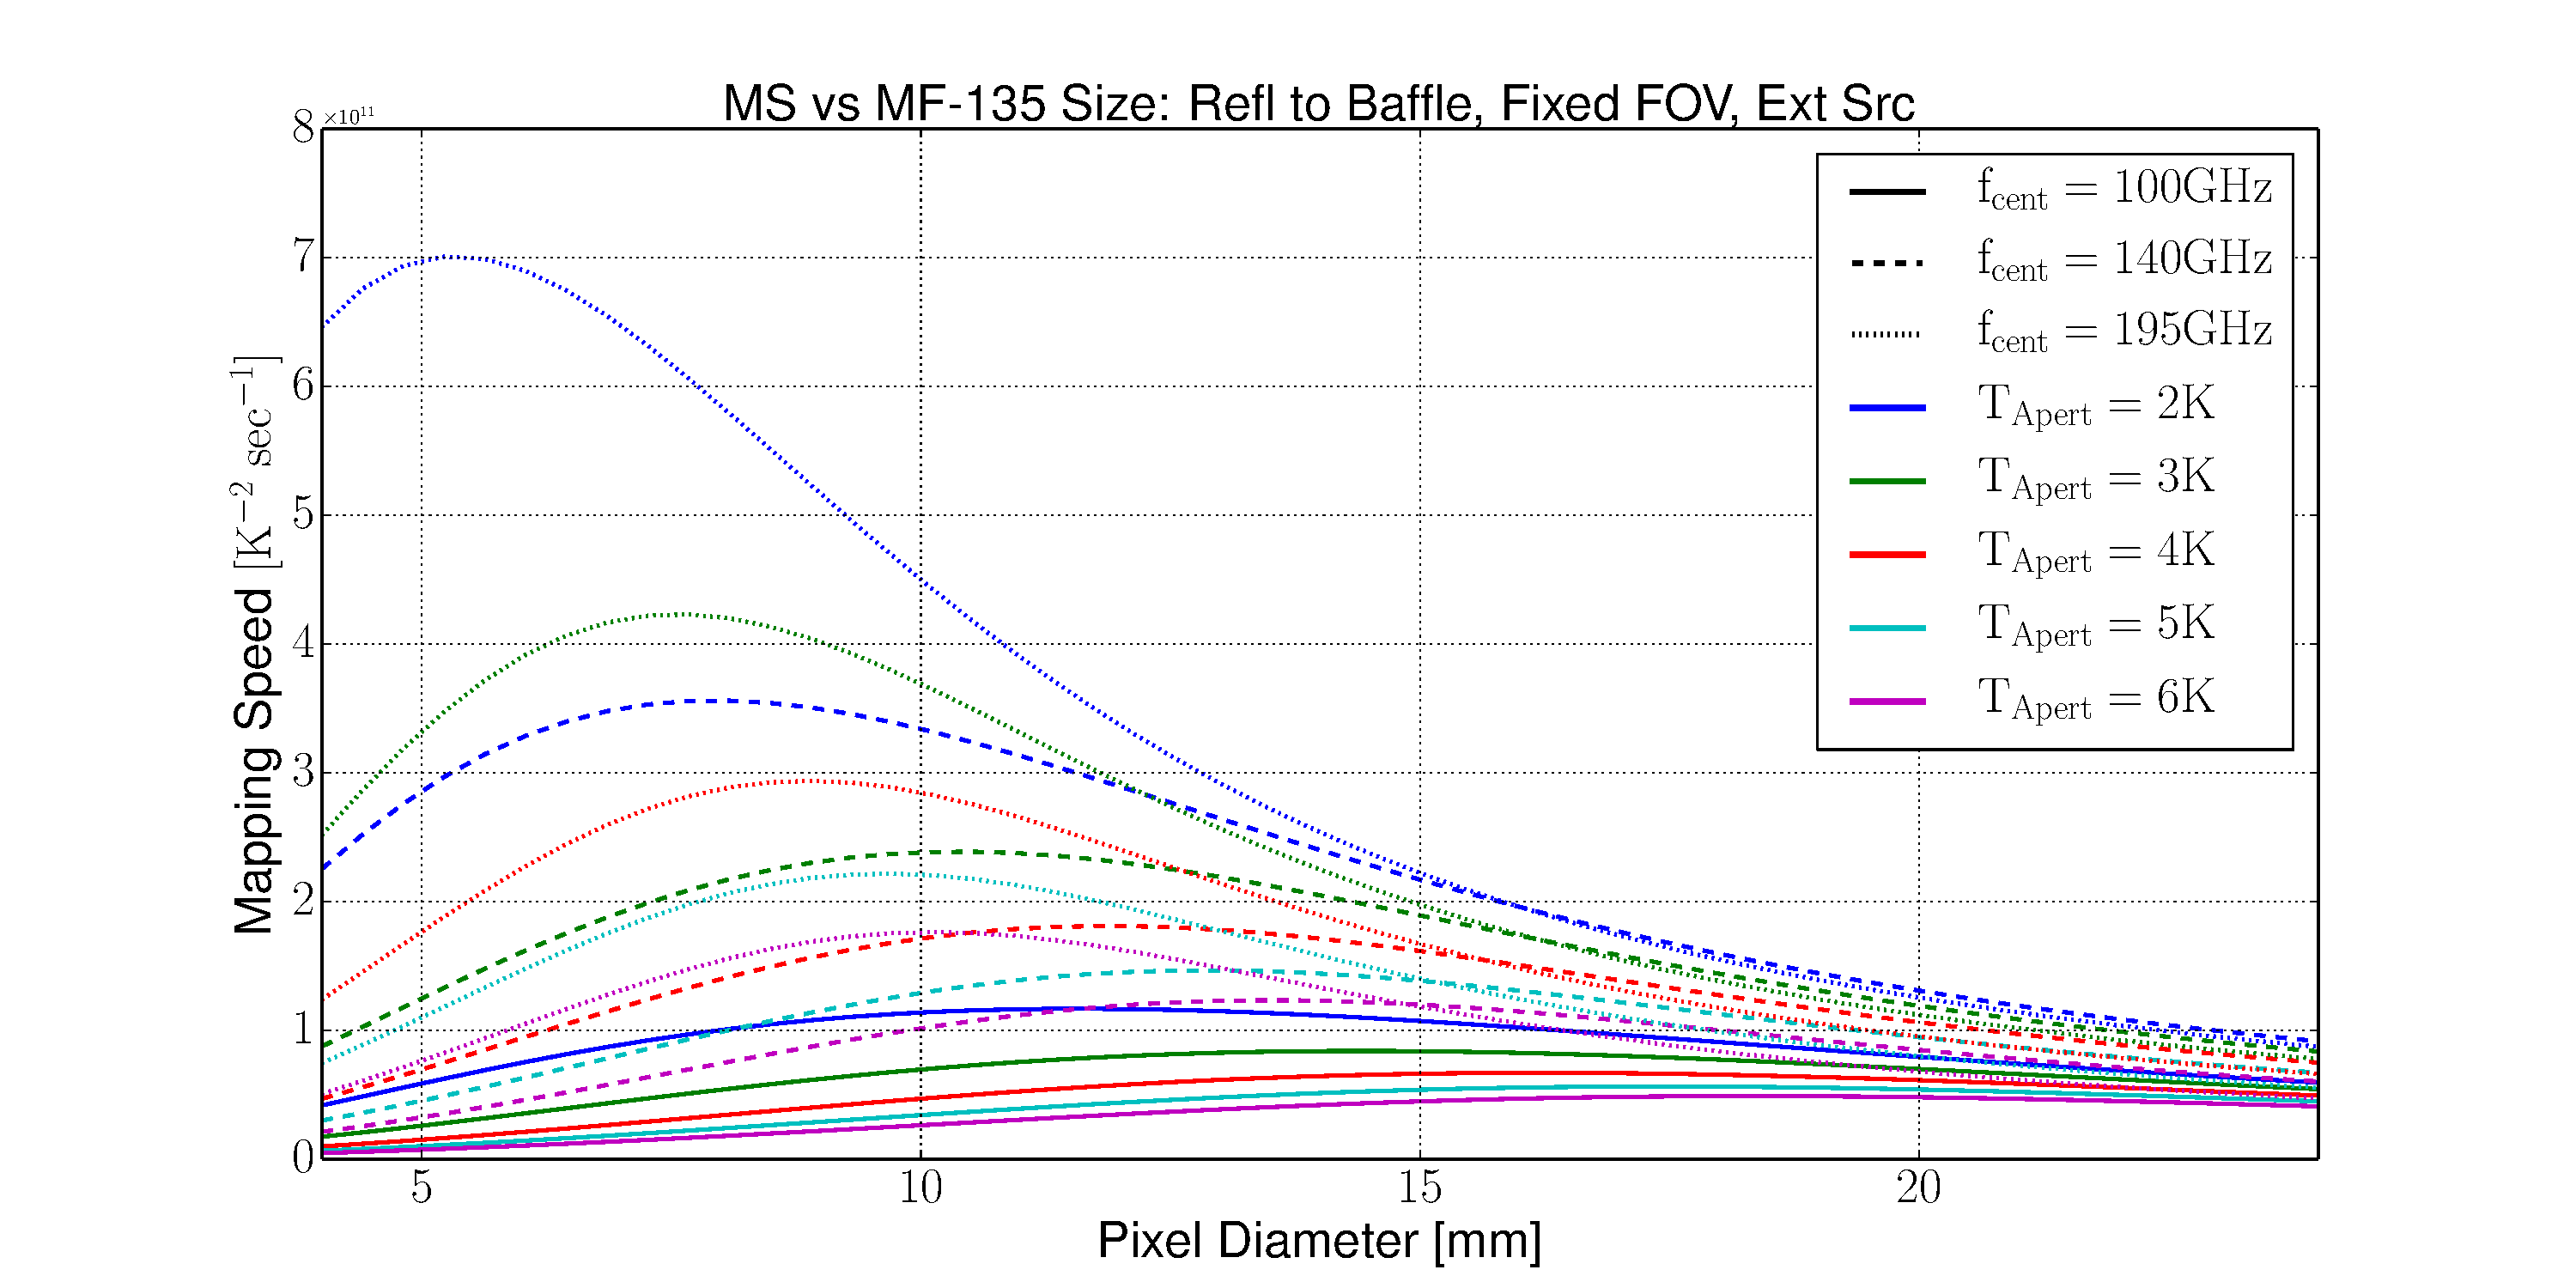
\includegraphics[width=1.1\textwidth, center]{PDF/LFT_MS_MF-135_hotRefl_fixFOV_extSrc.pdf}
	\caption{MF-135 mapping speed of an extended source as a function of pixel diameter for hot reflections and fixed FOV}
\end{figure}

\begin{figure}[H]
	\centering
	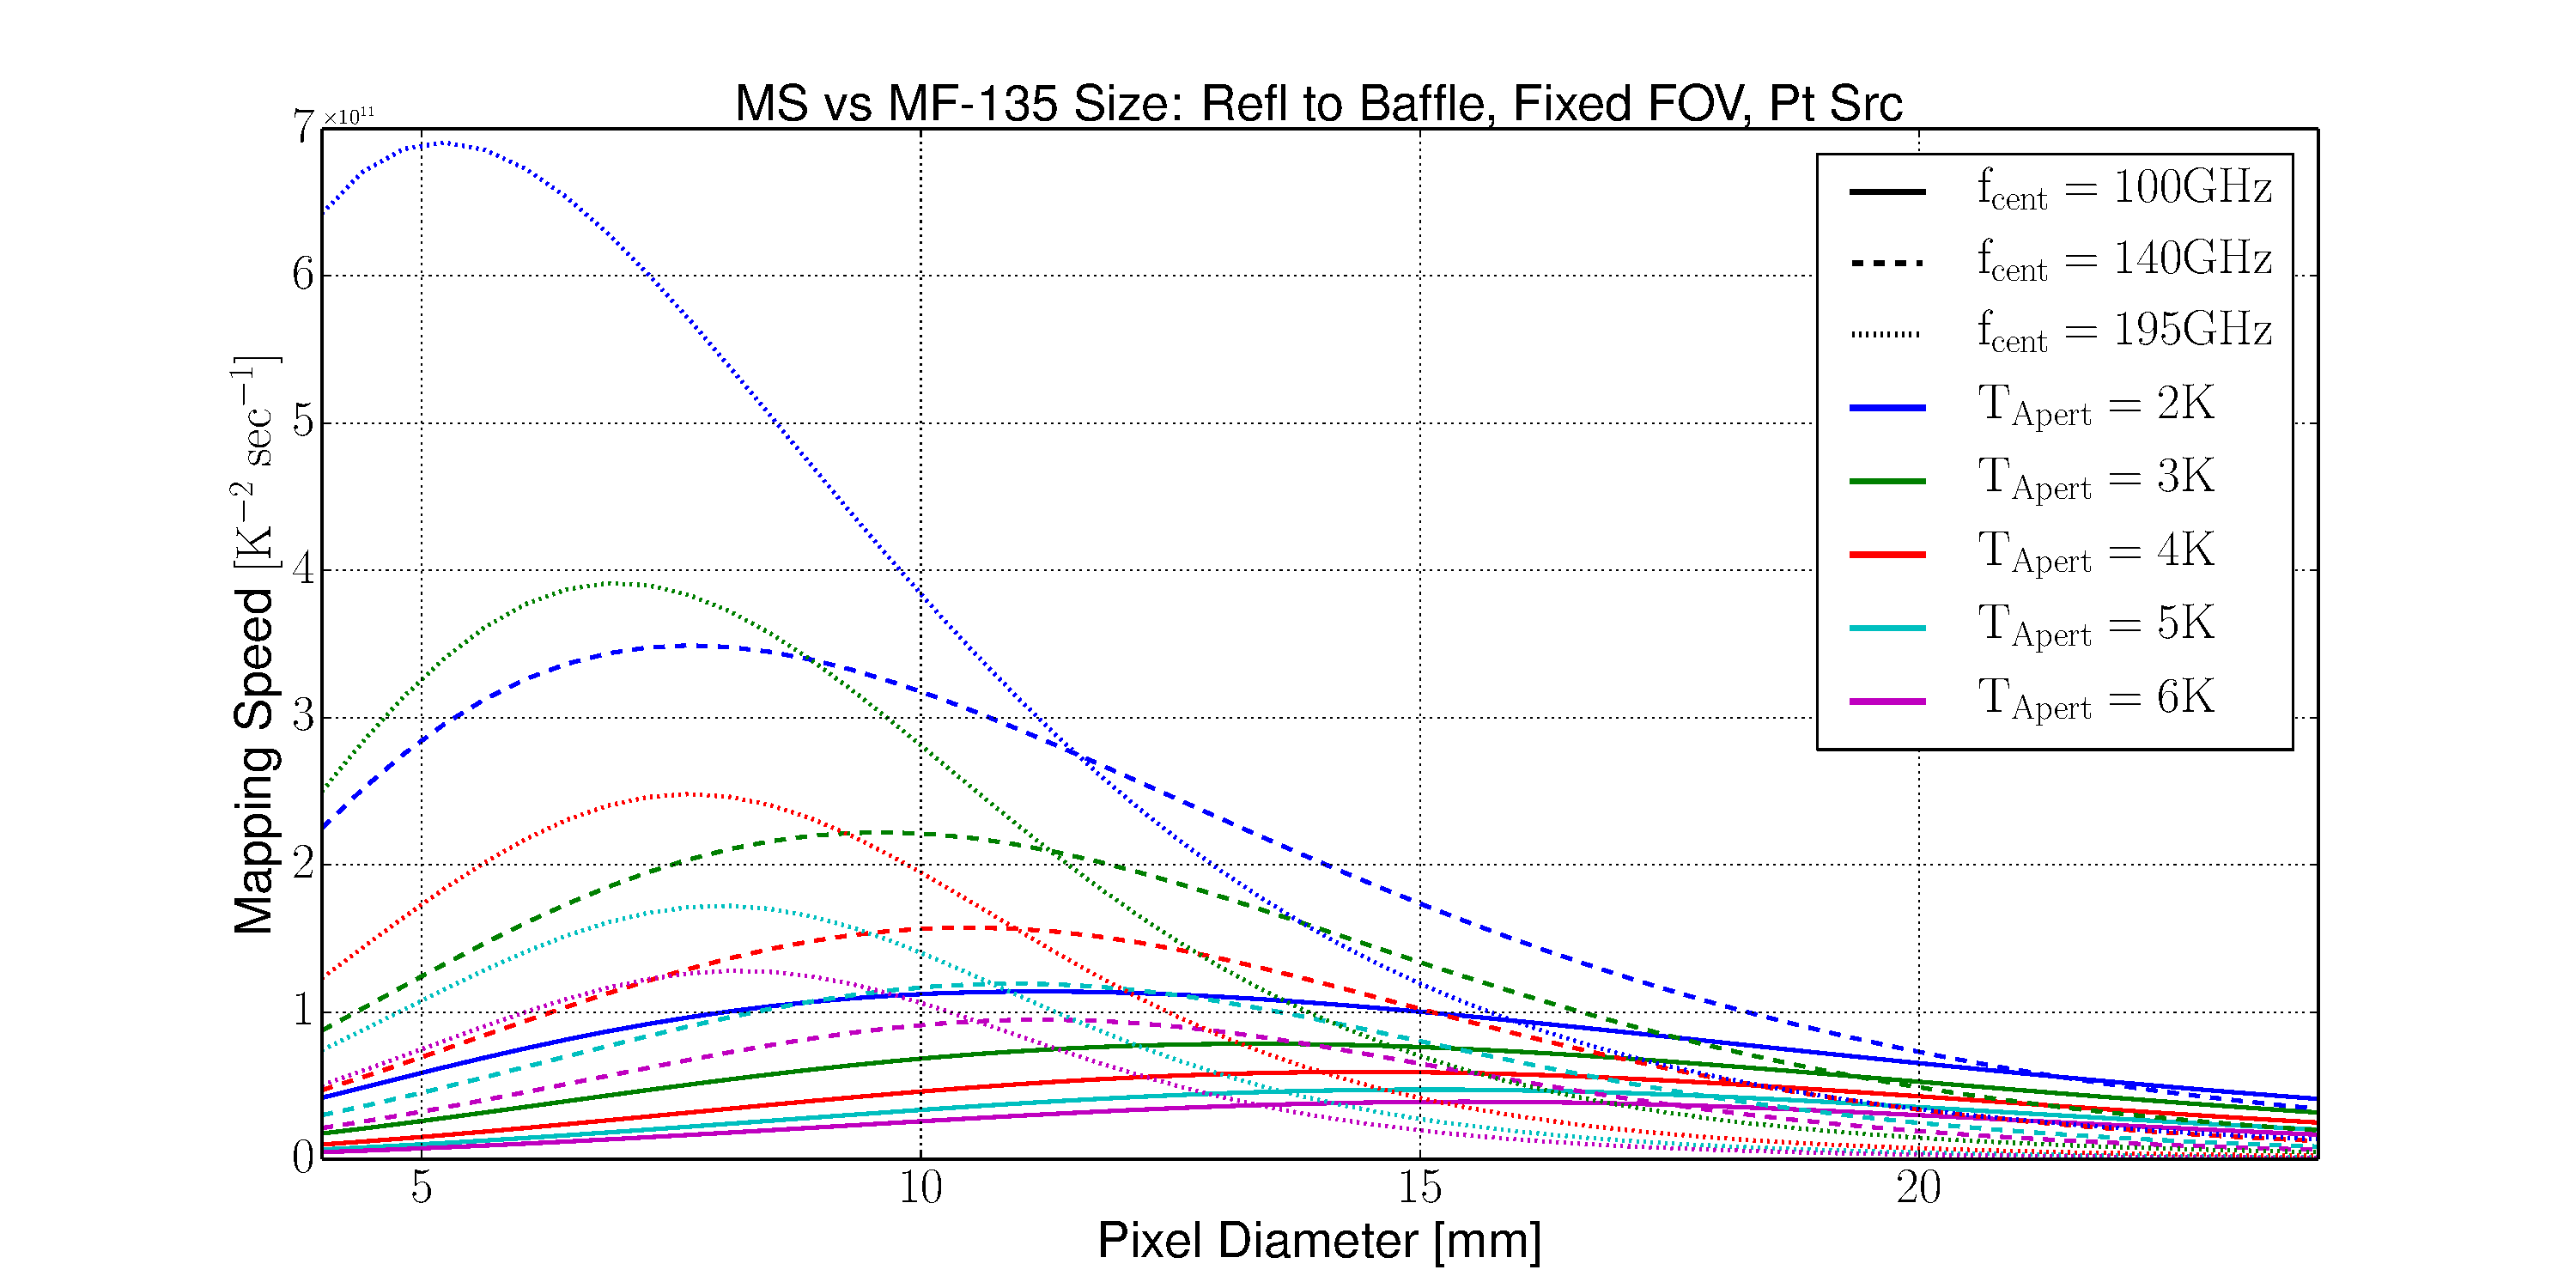
\includegraphics[width=1.1\textwidth, center]{PDF/LFT_MS_MF-135_hotRefl_fixFOV_ptSrc.pdf}
	\caption{MF-135 mapping speed of a point source as a function of pixel diameter for hot reflections and fixed FOV}
\end{figure}

%%%%%%%%%%%%%%%%%%% 

\subsubsection{MF-246}

\begin{figure}[H]
	\centering
	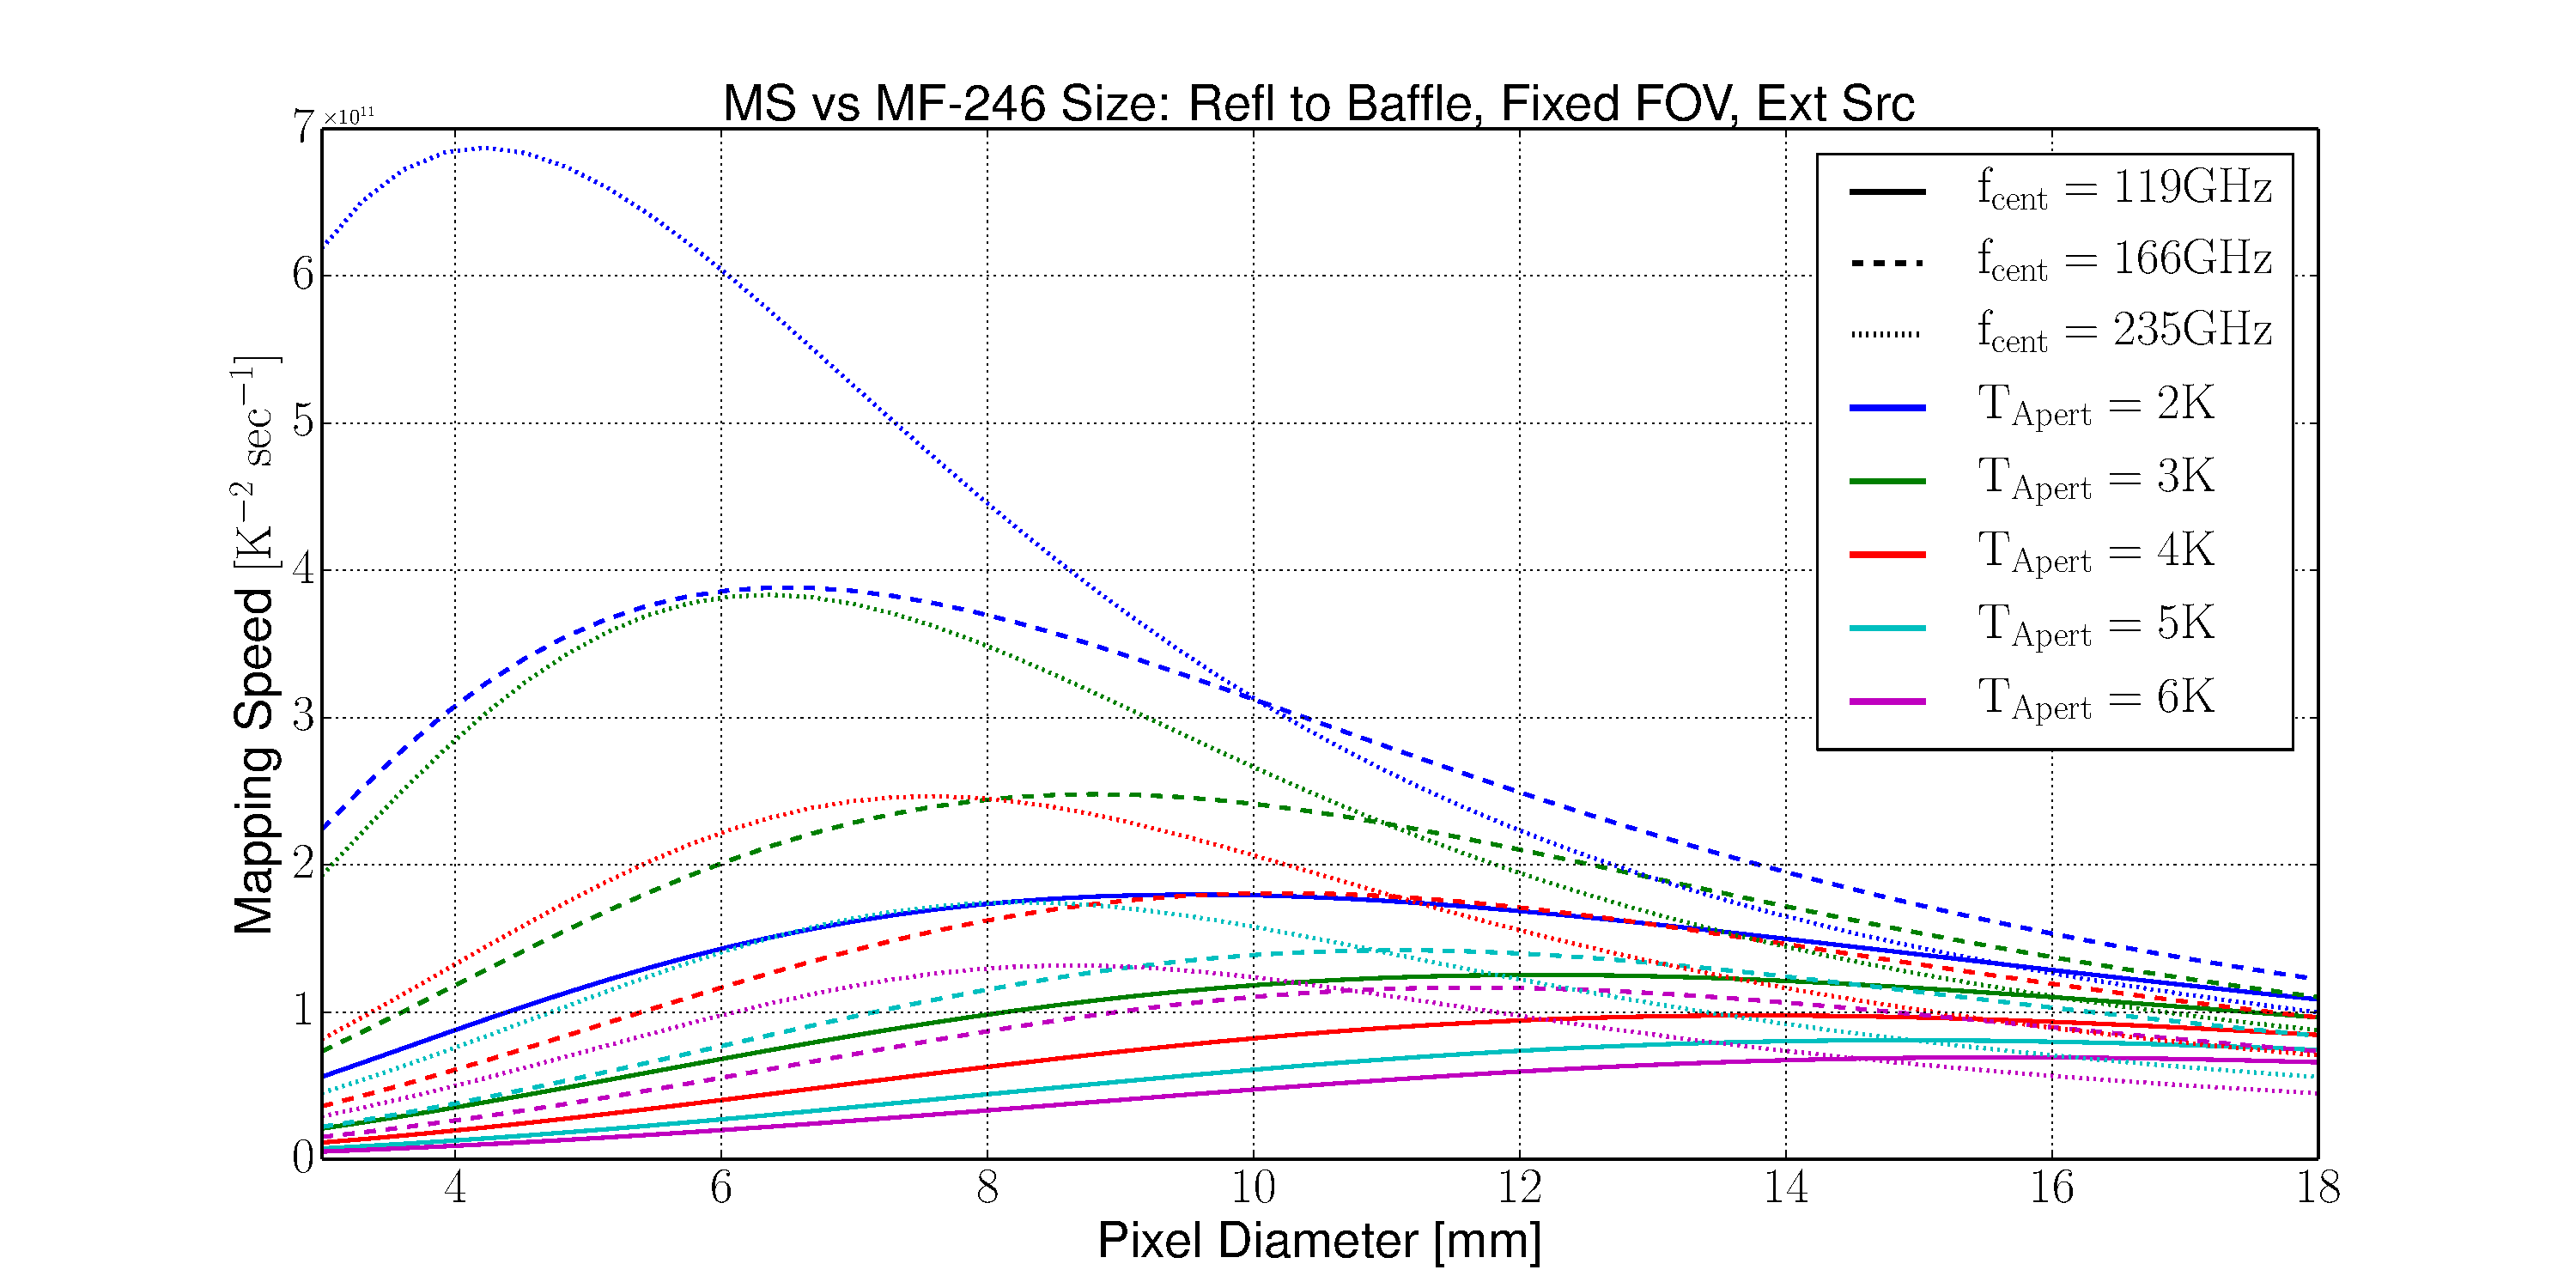
\includegraphics[width=1.1\textwidth, center]{PDF/LFT_MS_MF-246_hotRefl_fixFOV_extSrc.pdf}
	\caption{MF-246 mapping speed of an extended source as a function of pixel diameter for hot reflections and fixed FOV}
\end{figure}

\begin{figure}[H]
	\centering
	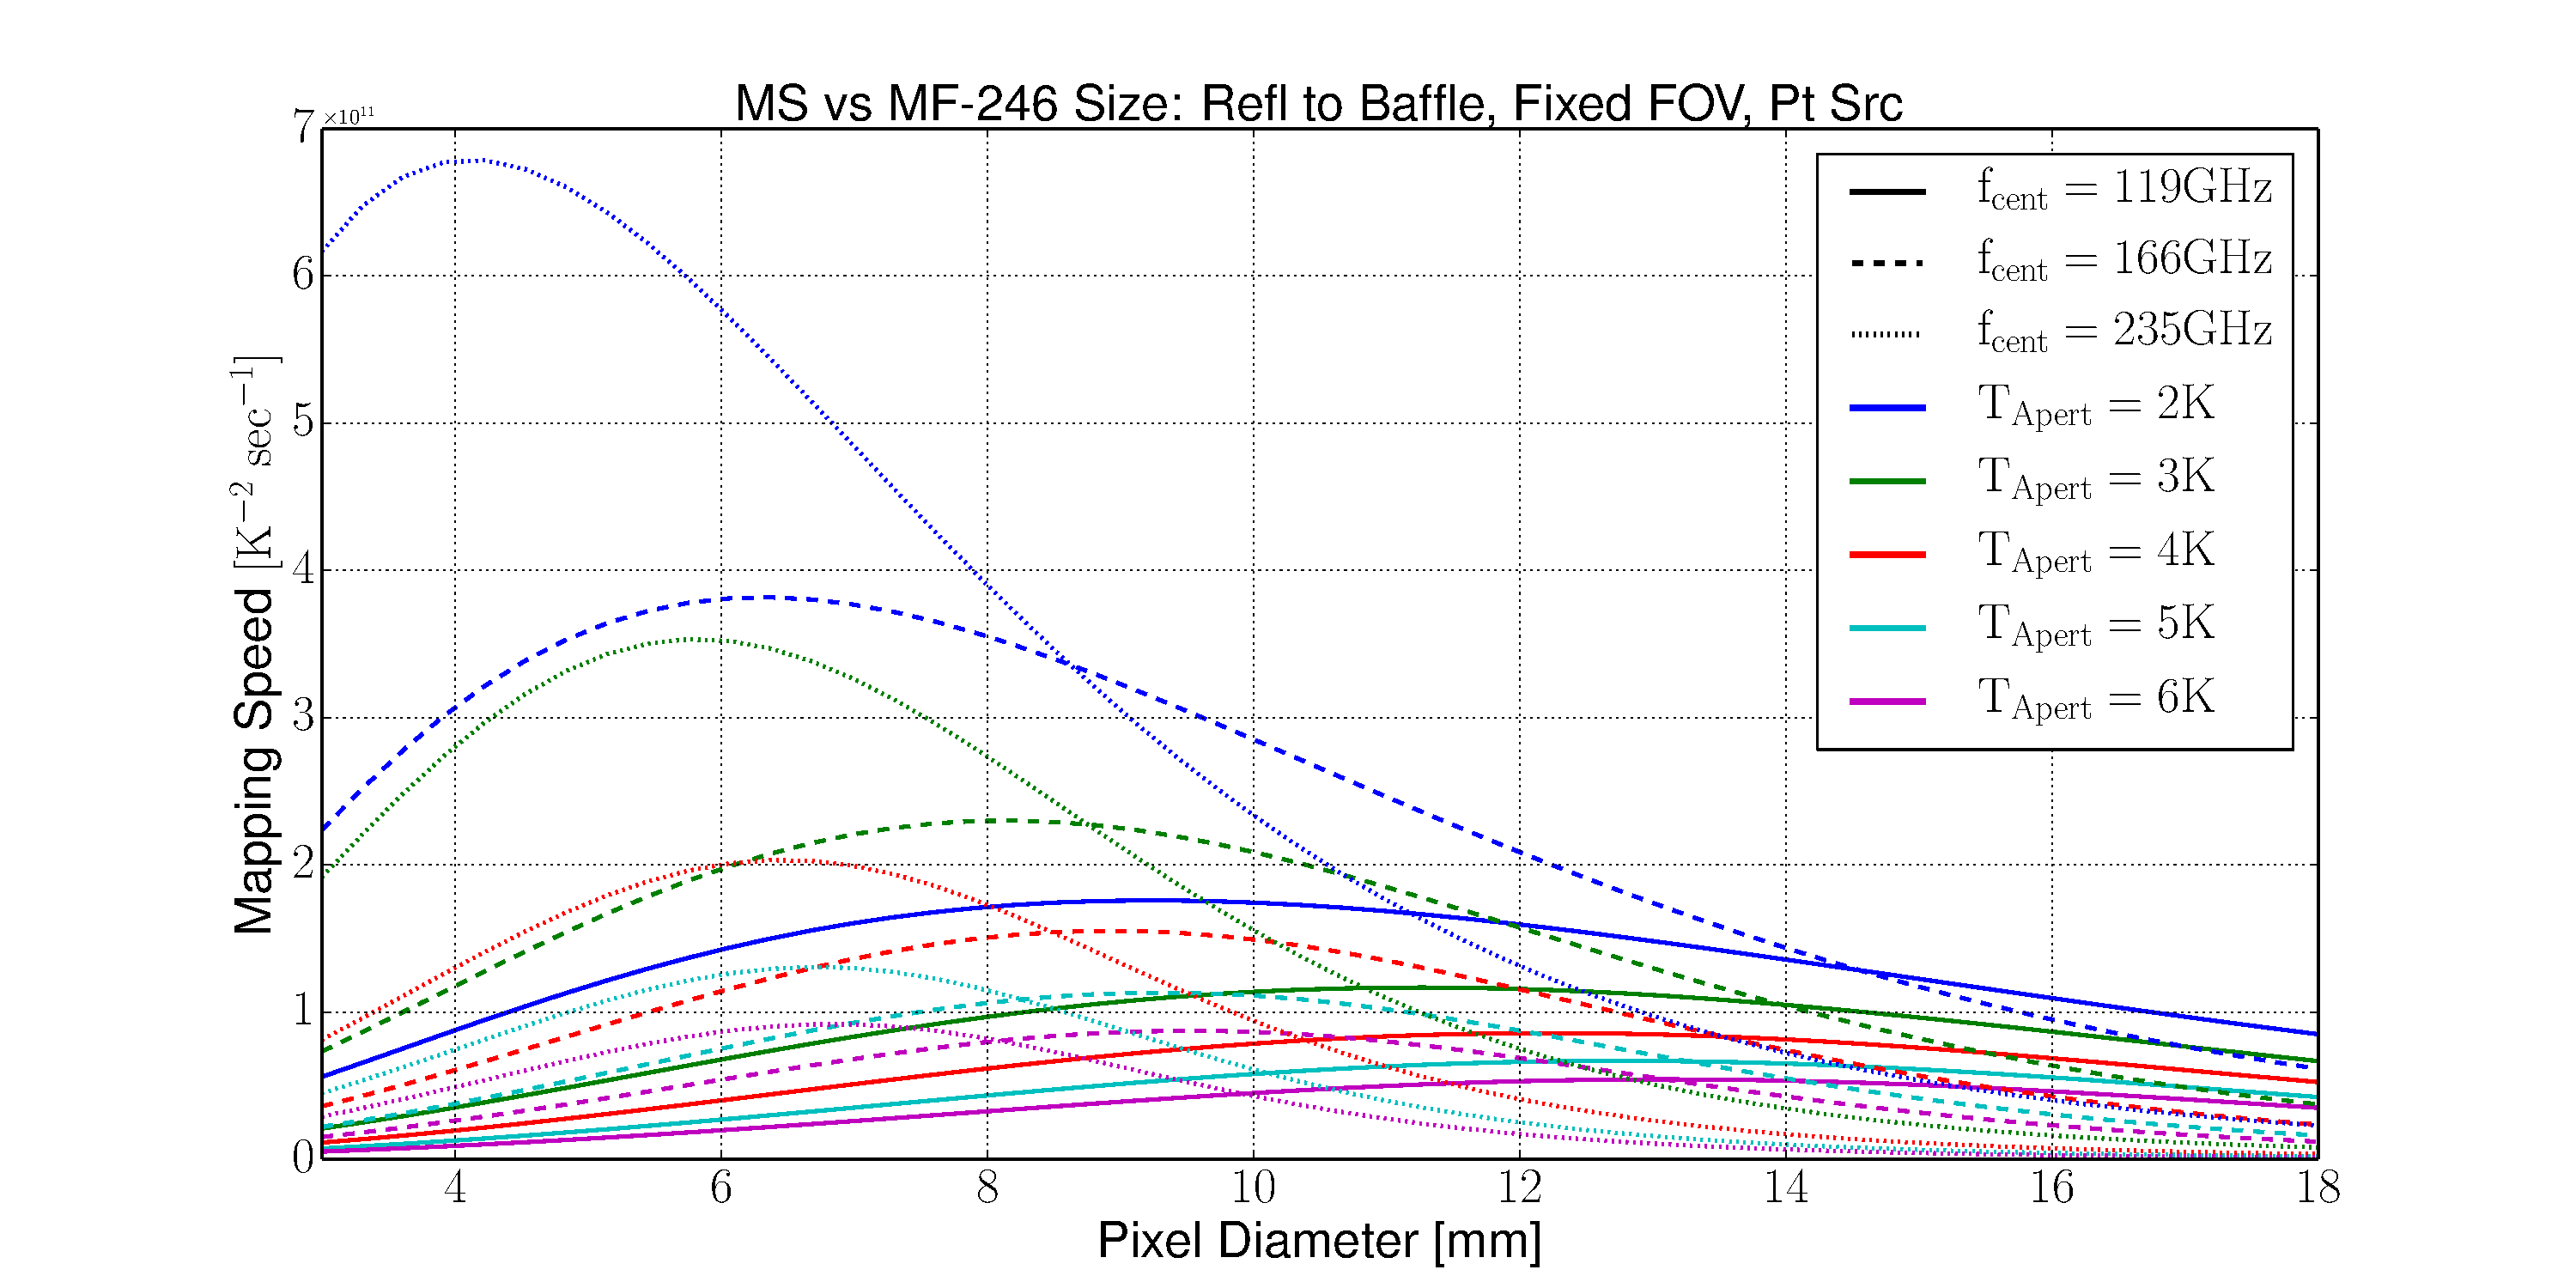
\includegraphics[width=1.1\textwidth, center]{PDF/LFT_MS_MF-246_hotRefl_fixFOV_ptSrc.pdf}
	\caption{MF-246 mapping speed of a point source as a function of pixel diameter for hot reflections and fixed FOV}
\end{figure}

%%%%%%%%%%%%%%%%%%%

\subsubsection{HFT}

\begin{figure}[H]
	\centering
	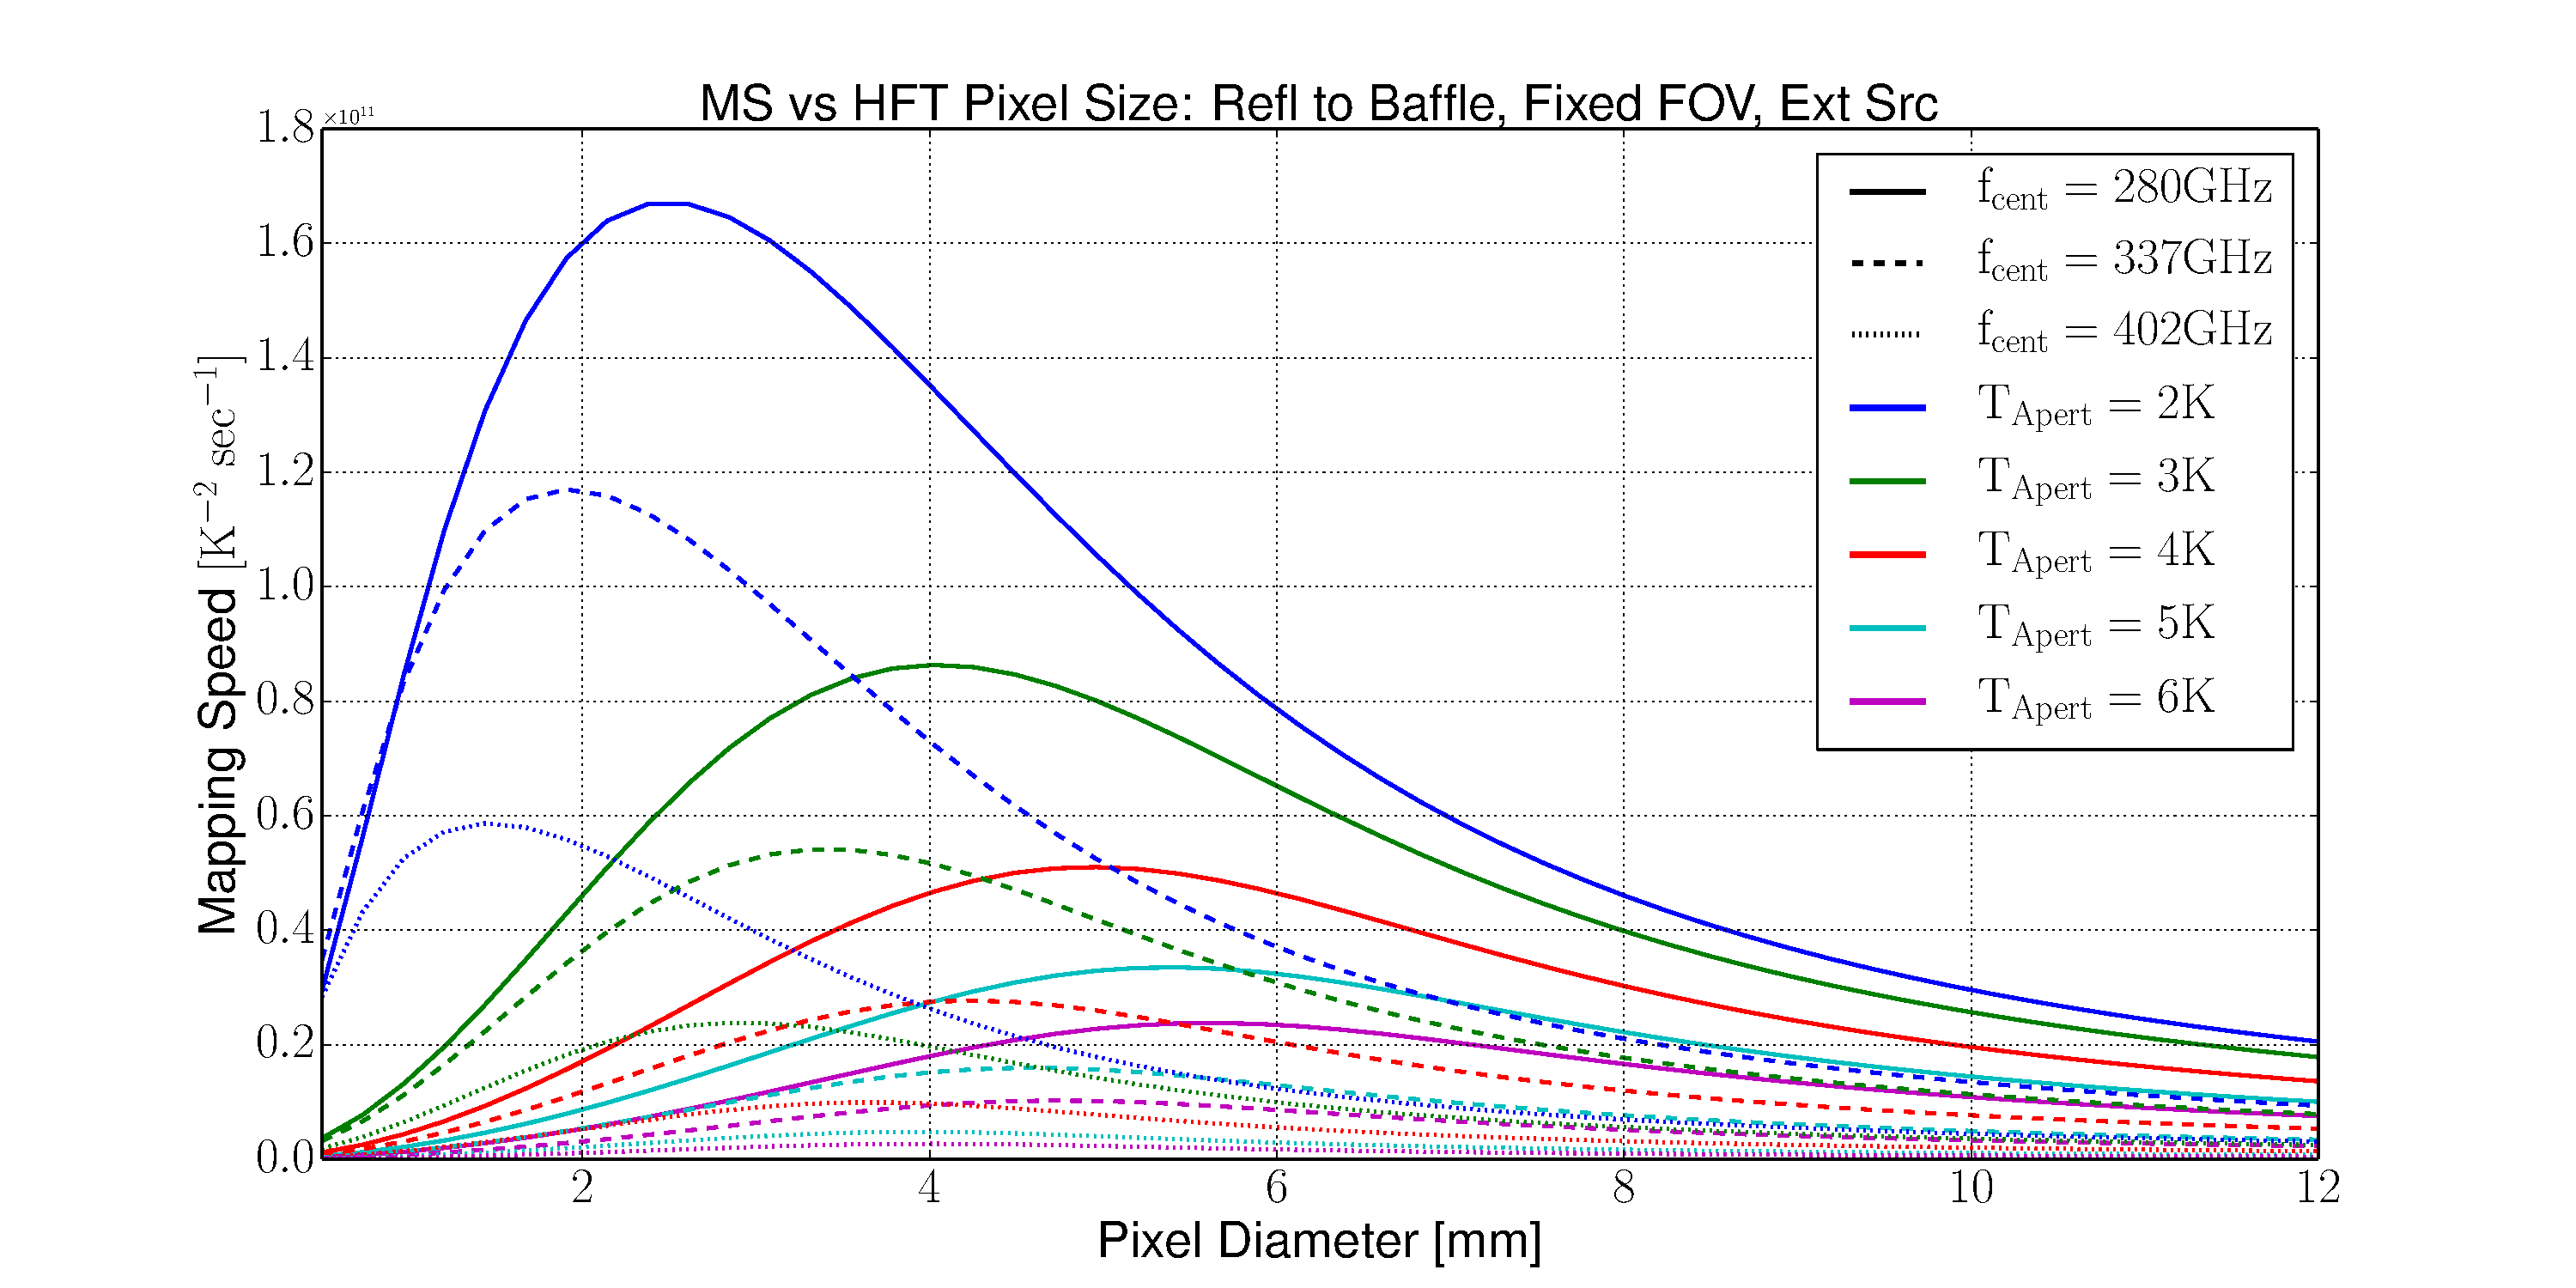
\includegraphics[width=1.1\textwidth, center]{PDF/HFT_MS_hotRefl_fixFOV_extSrc.pdf}
	\caption{HFT mapping speed of an extended source as a function of pixel diameter for hot reflections and fixed FOV}
\end{figure}

\begin{figure}[H]
	\centering
	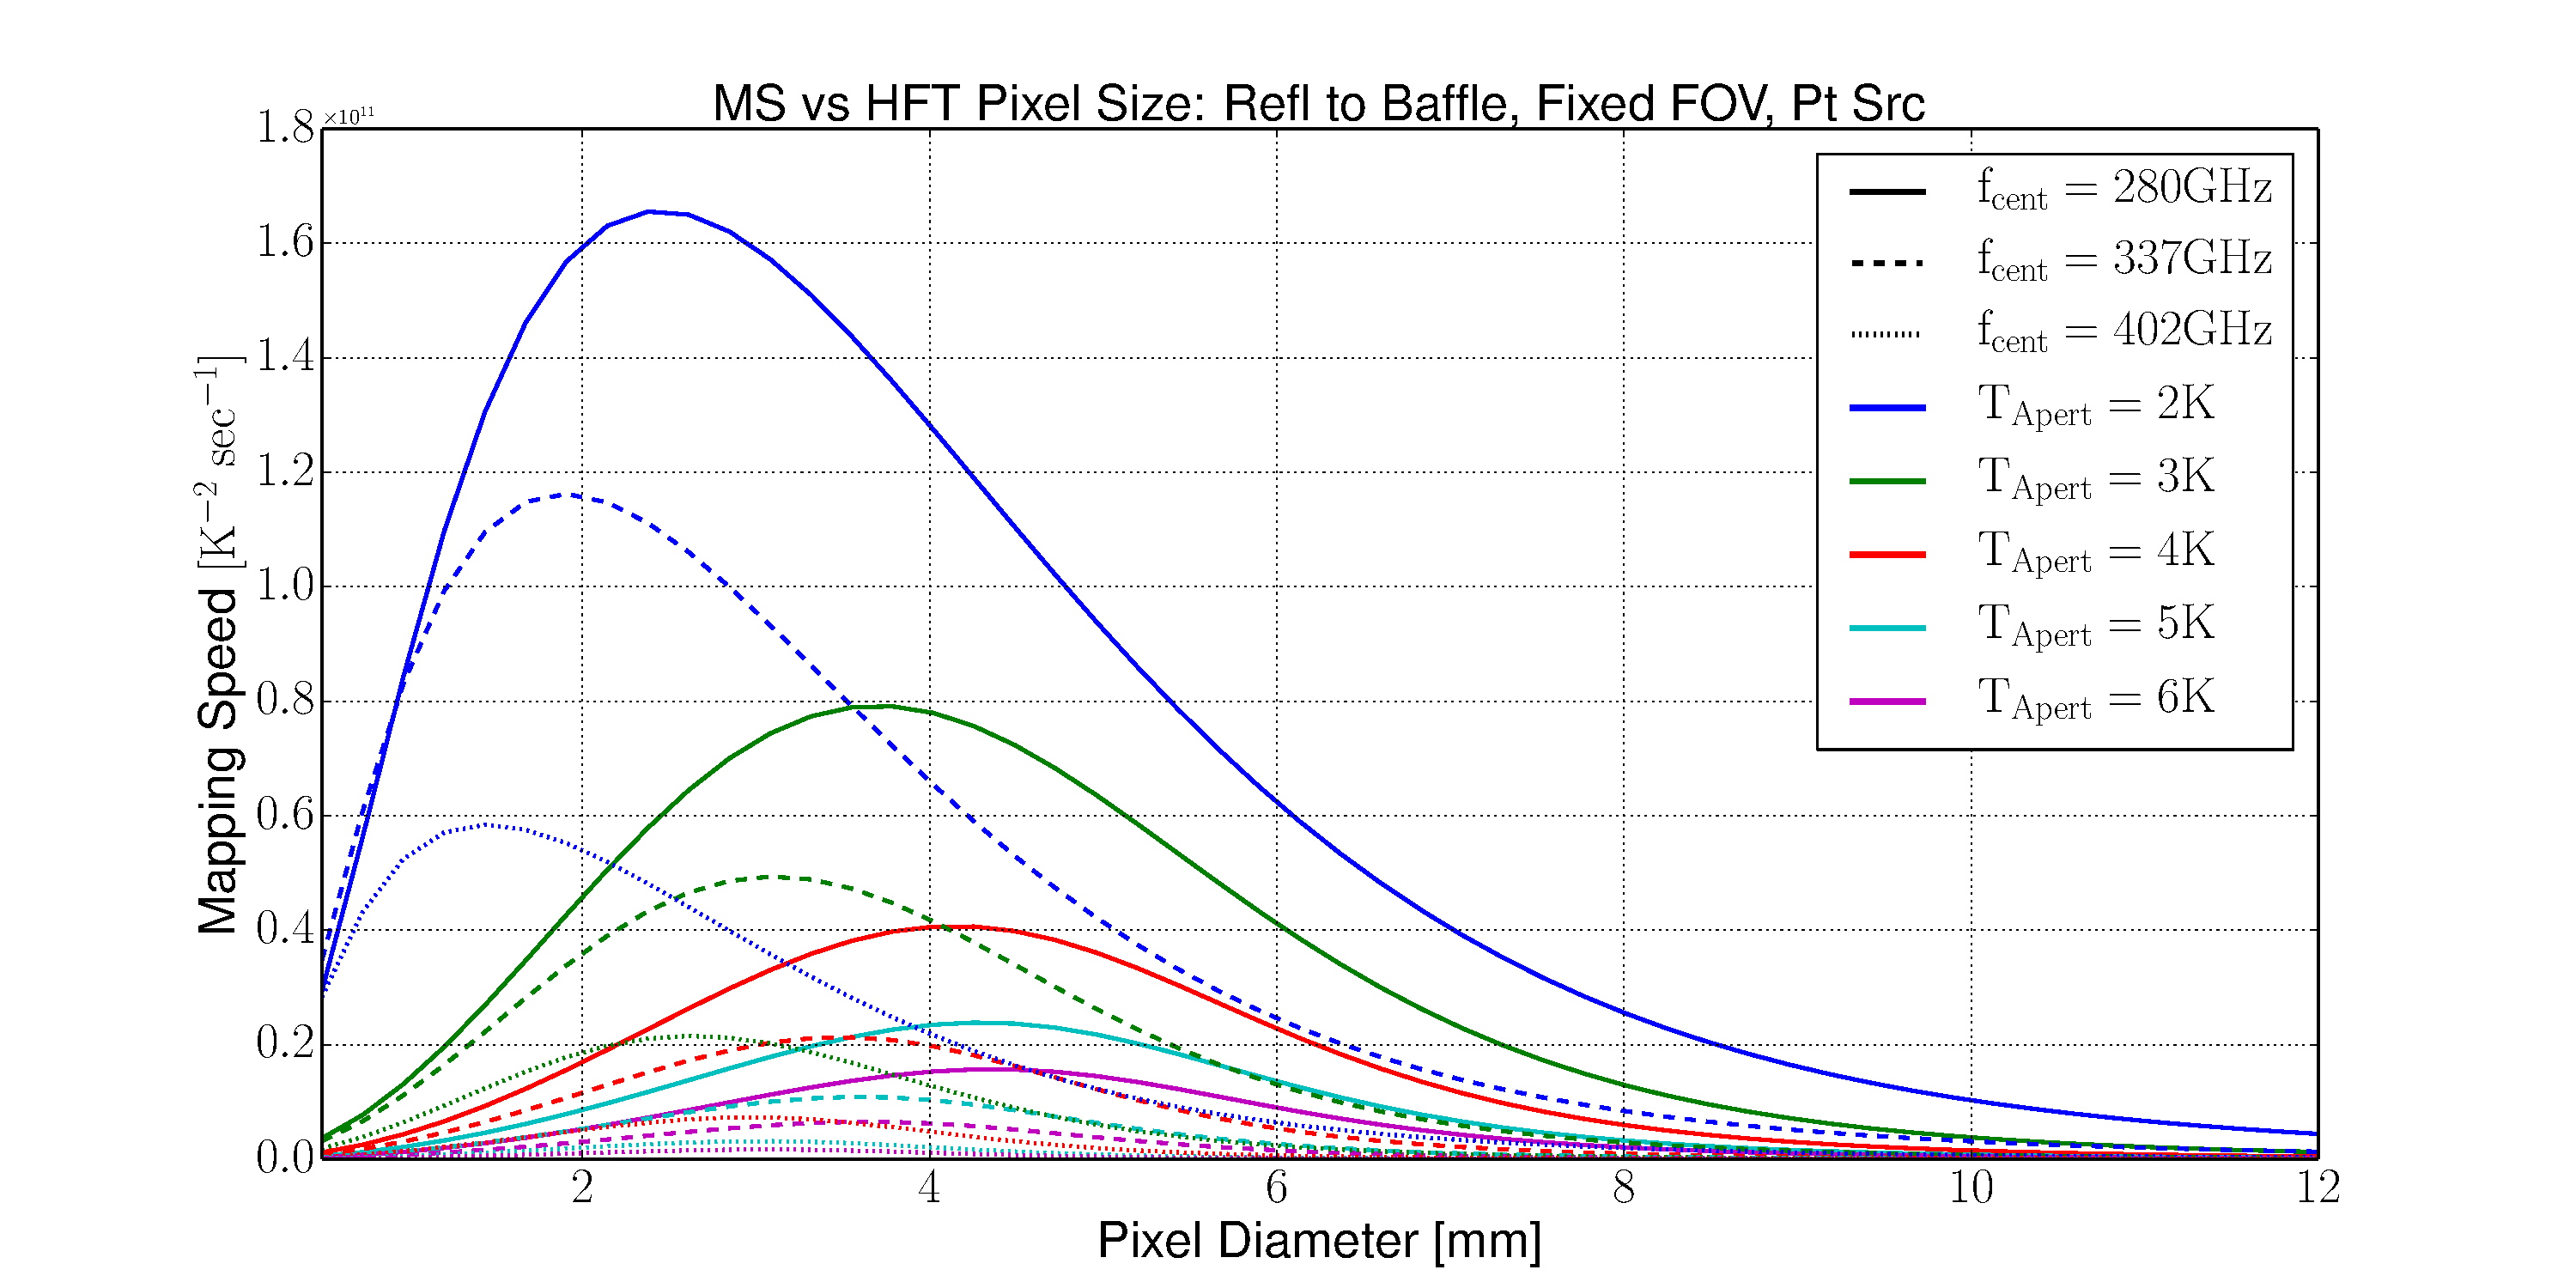
\includegraphics[width=1.1\textwidth, center]{PDF/HFT_MS_hotRefl_fixFOV_ptSrc.pdf}
	\caption{HFT mapping speed of a point source as a function of pixel diameter for hot reflections and fixed FOV}
\end{figure}


%%%%%%%%%%%%%%%%%%%%%%%%%%%%%%%%%%%%%

\subsection{Reflections Go to Baffle, Fixed Number of Detectors}

This subsection containts the results for the optimization of pixel diameters for the LFT and HFT given a fixed number of detectors and assuming all reflections go to the baffling.

\clearpage

%%%%%%%%%%%%%%%%%%%

\subsubsection{LF-135}

\begin{figure}[H]
	\centering
	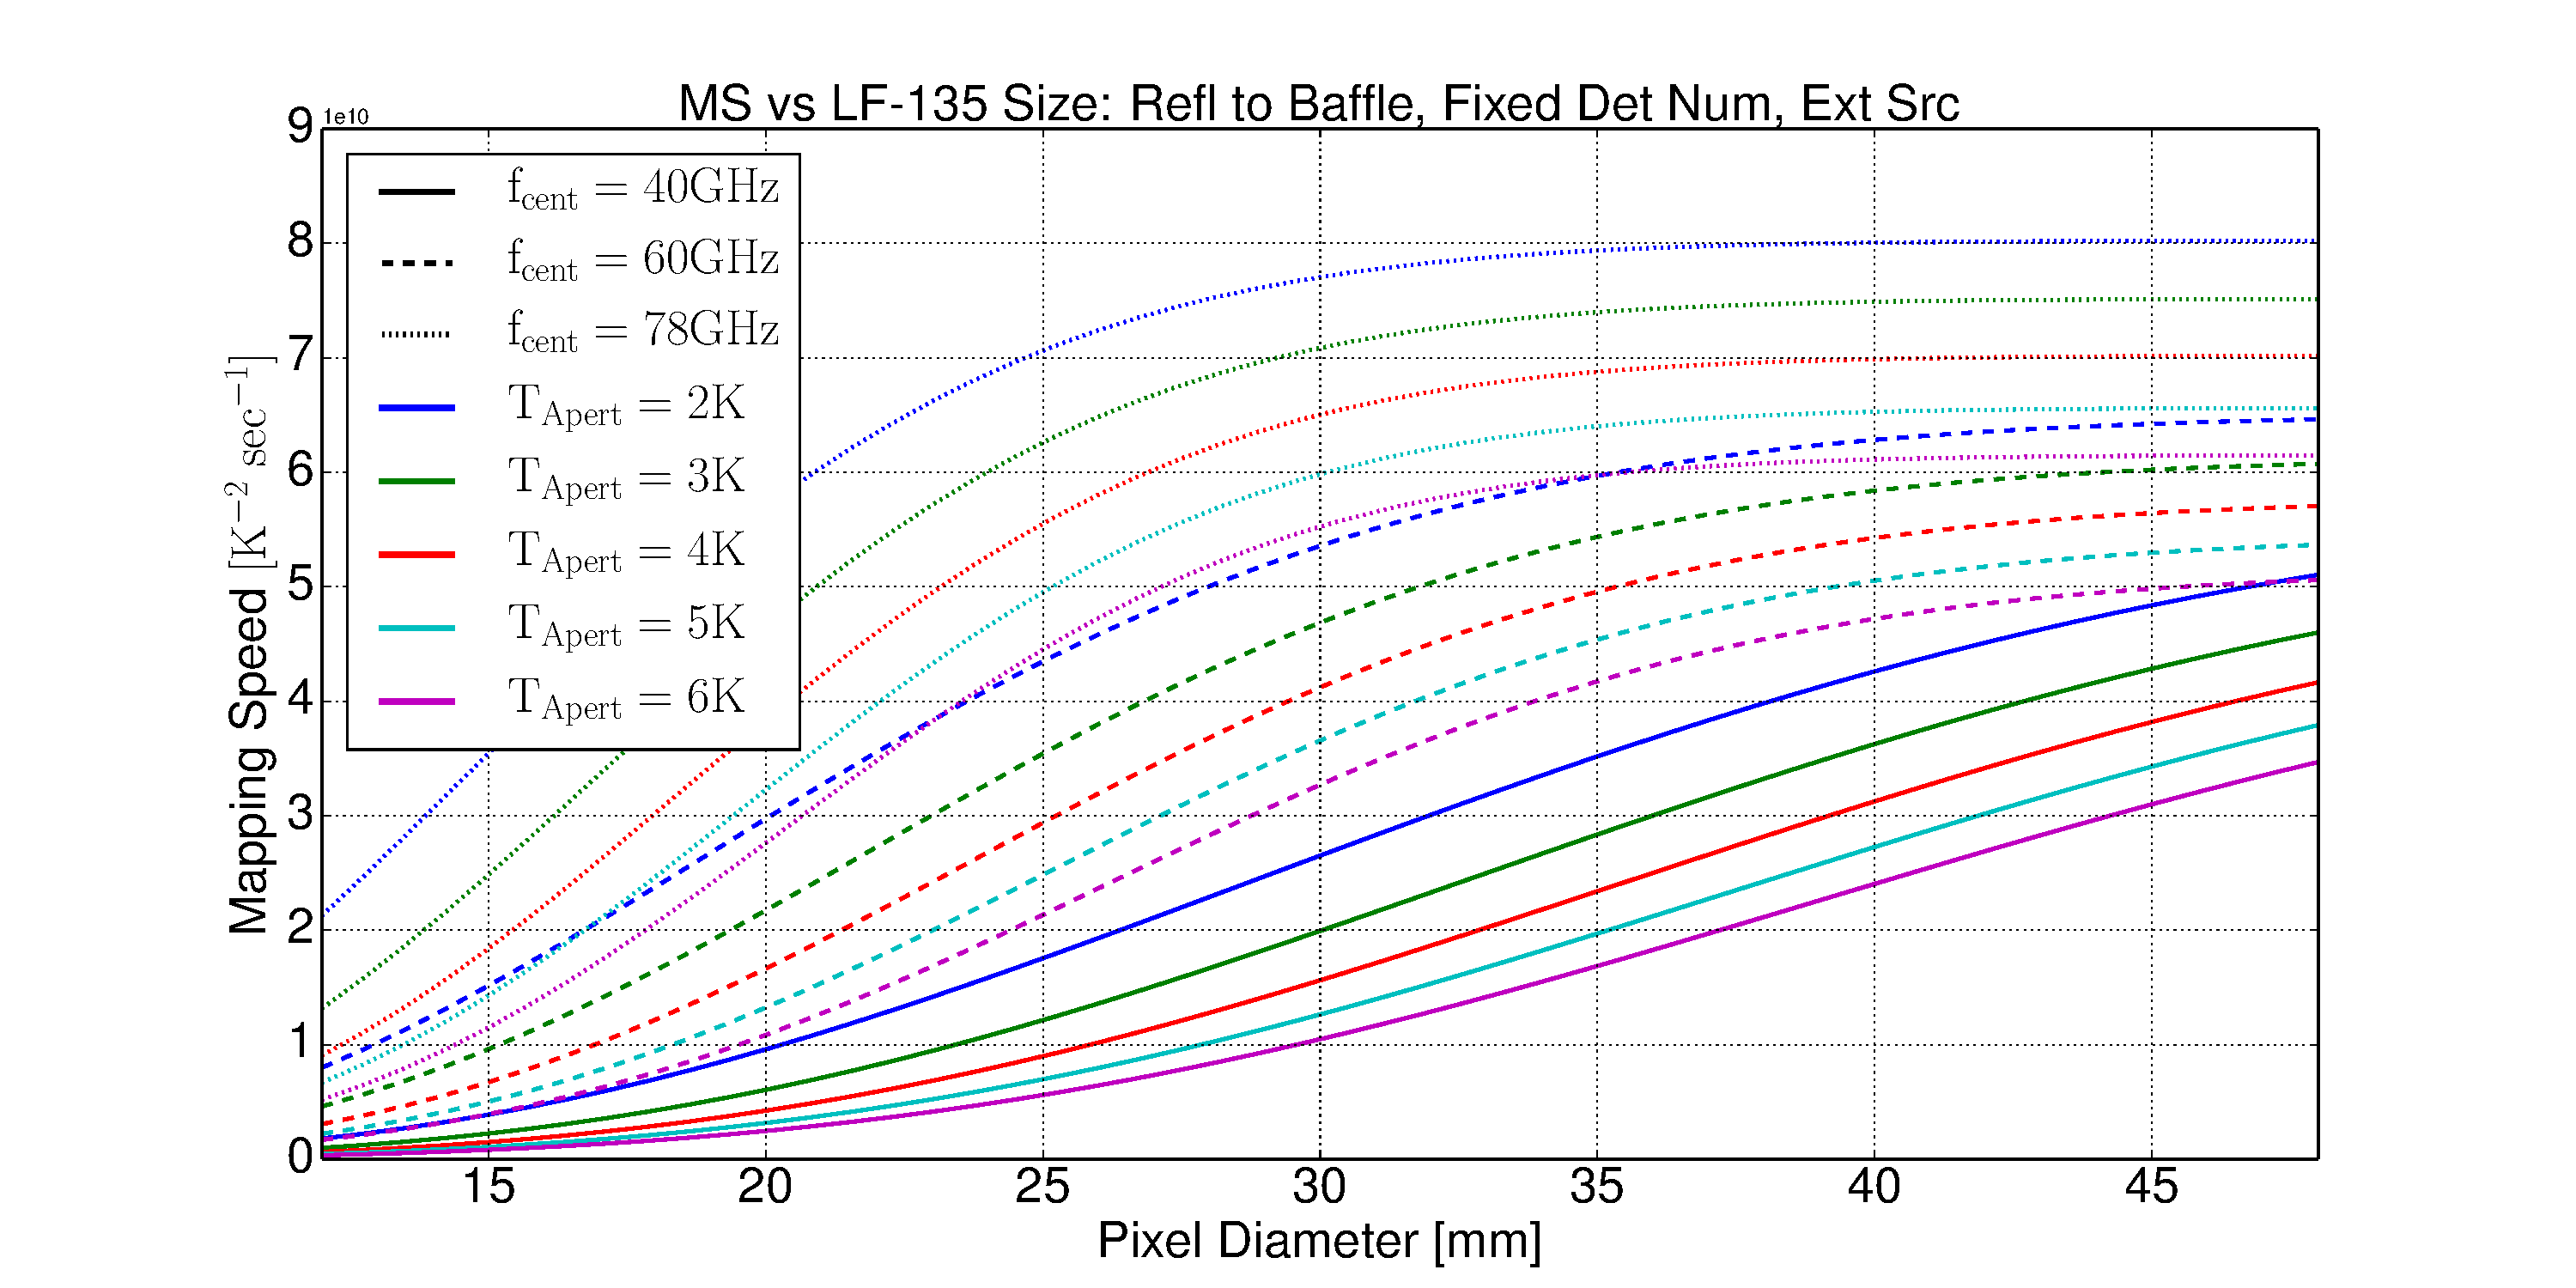
\includegraphics[width=1.1\textwidth, center]{PDF/LFT_MS_LF-135_hotRefl_fixDetNum_extSrc.pdf}
	\caption{LF-135 mapping speed of an extended source as a function of pixel diameter for hot reflections and fixed number of detectors}
\end{figure}

\begin{figure}[H]
	\centering
	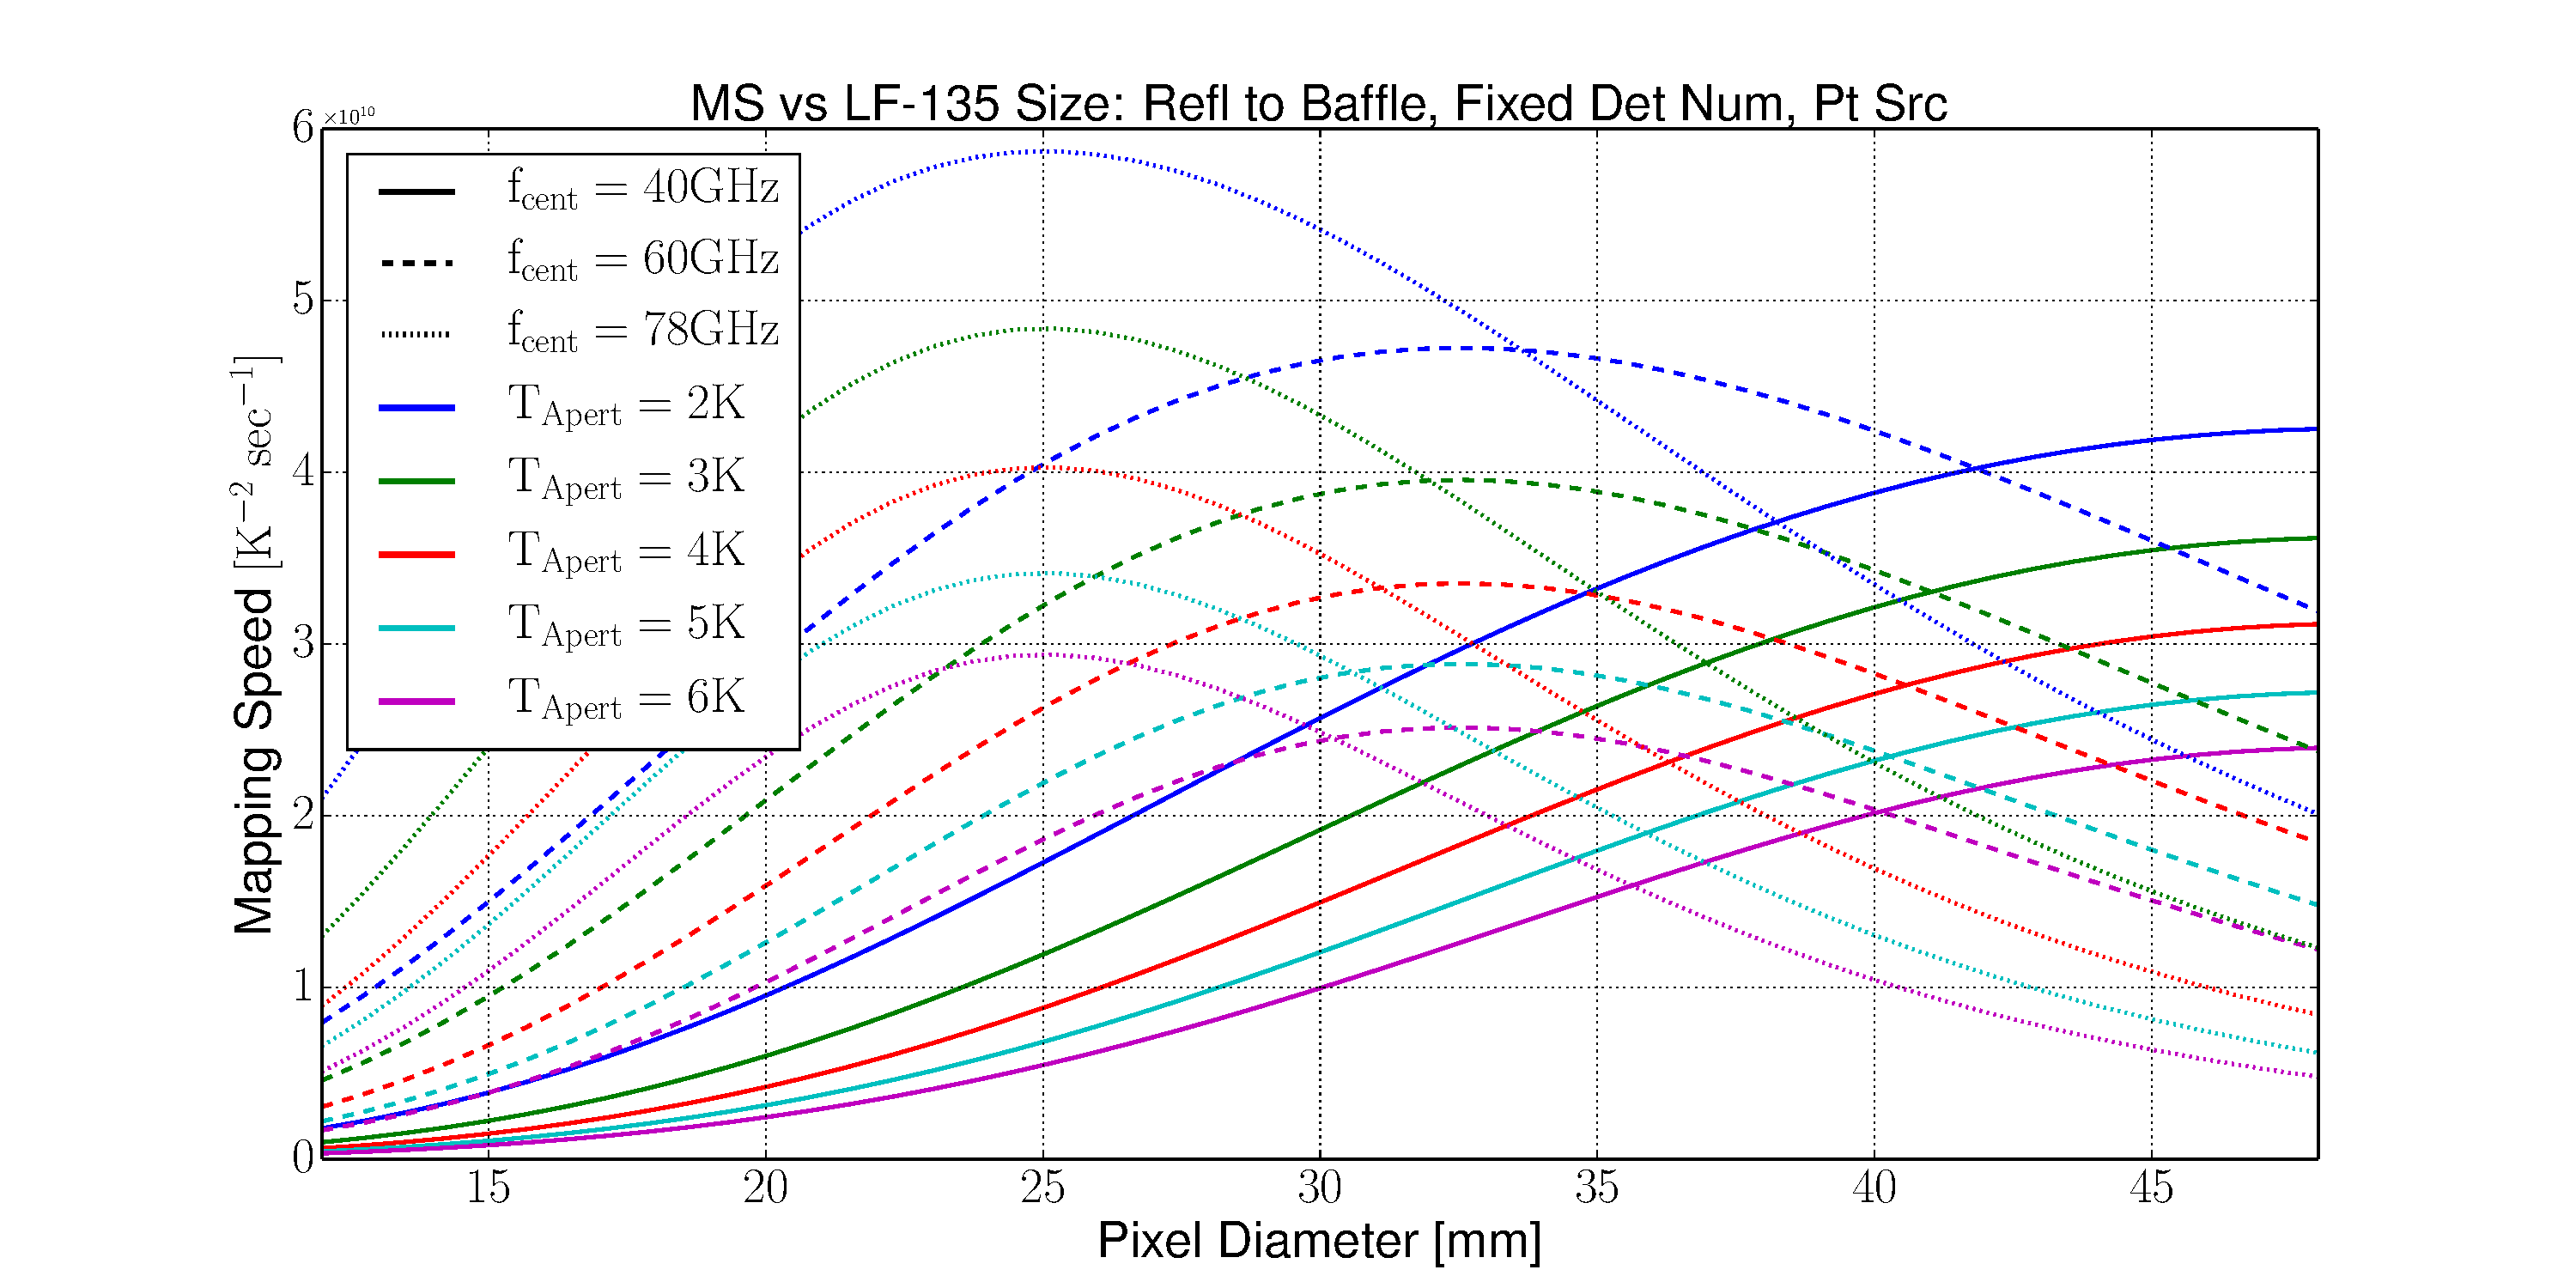
\includegraphics[width=1.1\textwidth, center]{PDF/LFT_MS_LF-135_hotRefl_fixDetNum_ptSrc.pdf}
	\caption{LF-135 mapping speed of a point source as a function of pixel diameter for hot reflections and fixed number of detectors}
\end{figure}

%%%%%%%%%%%%%%%%%%%

\subsubsection{LF-246}

\begin{figure}[H]
	\centering
	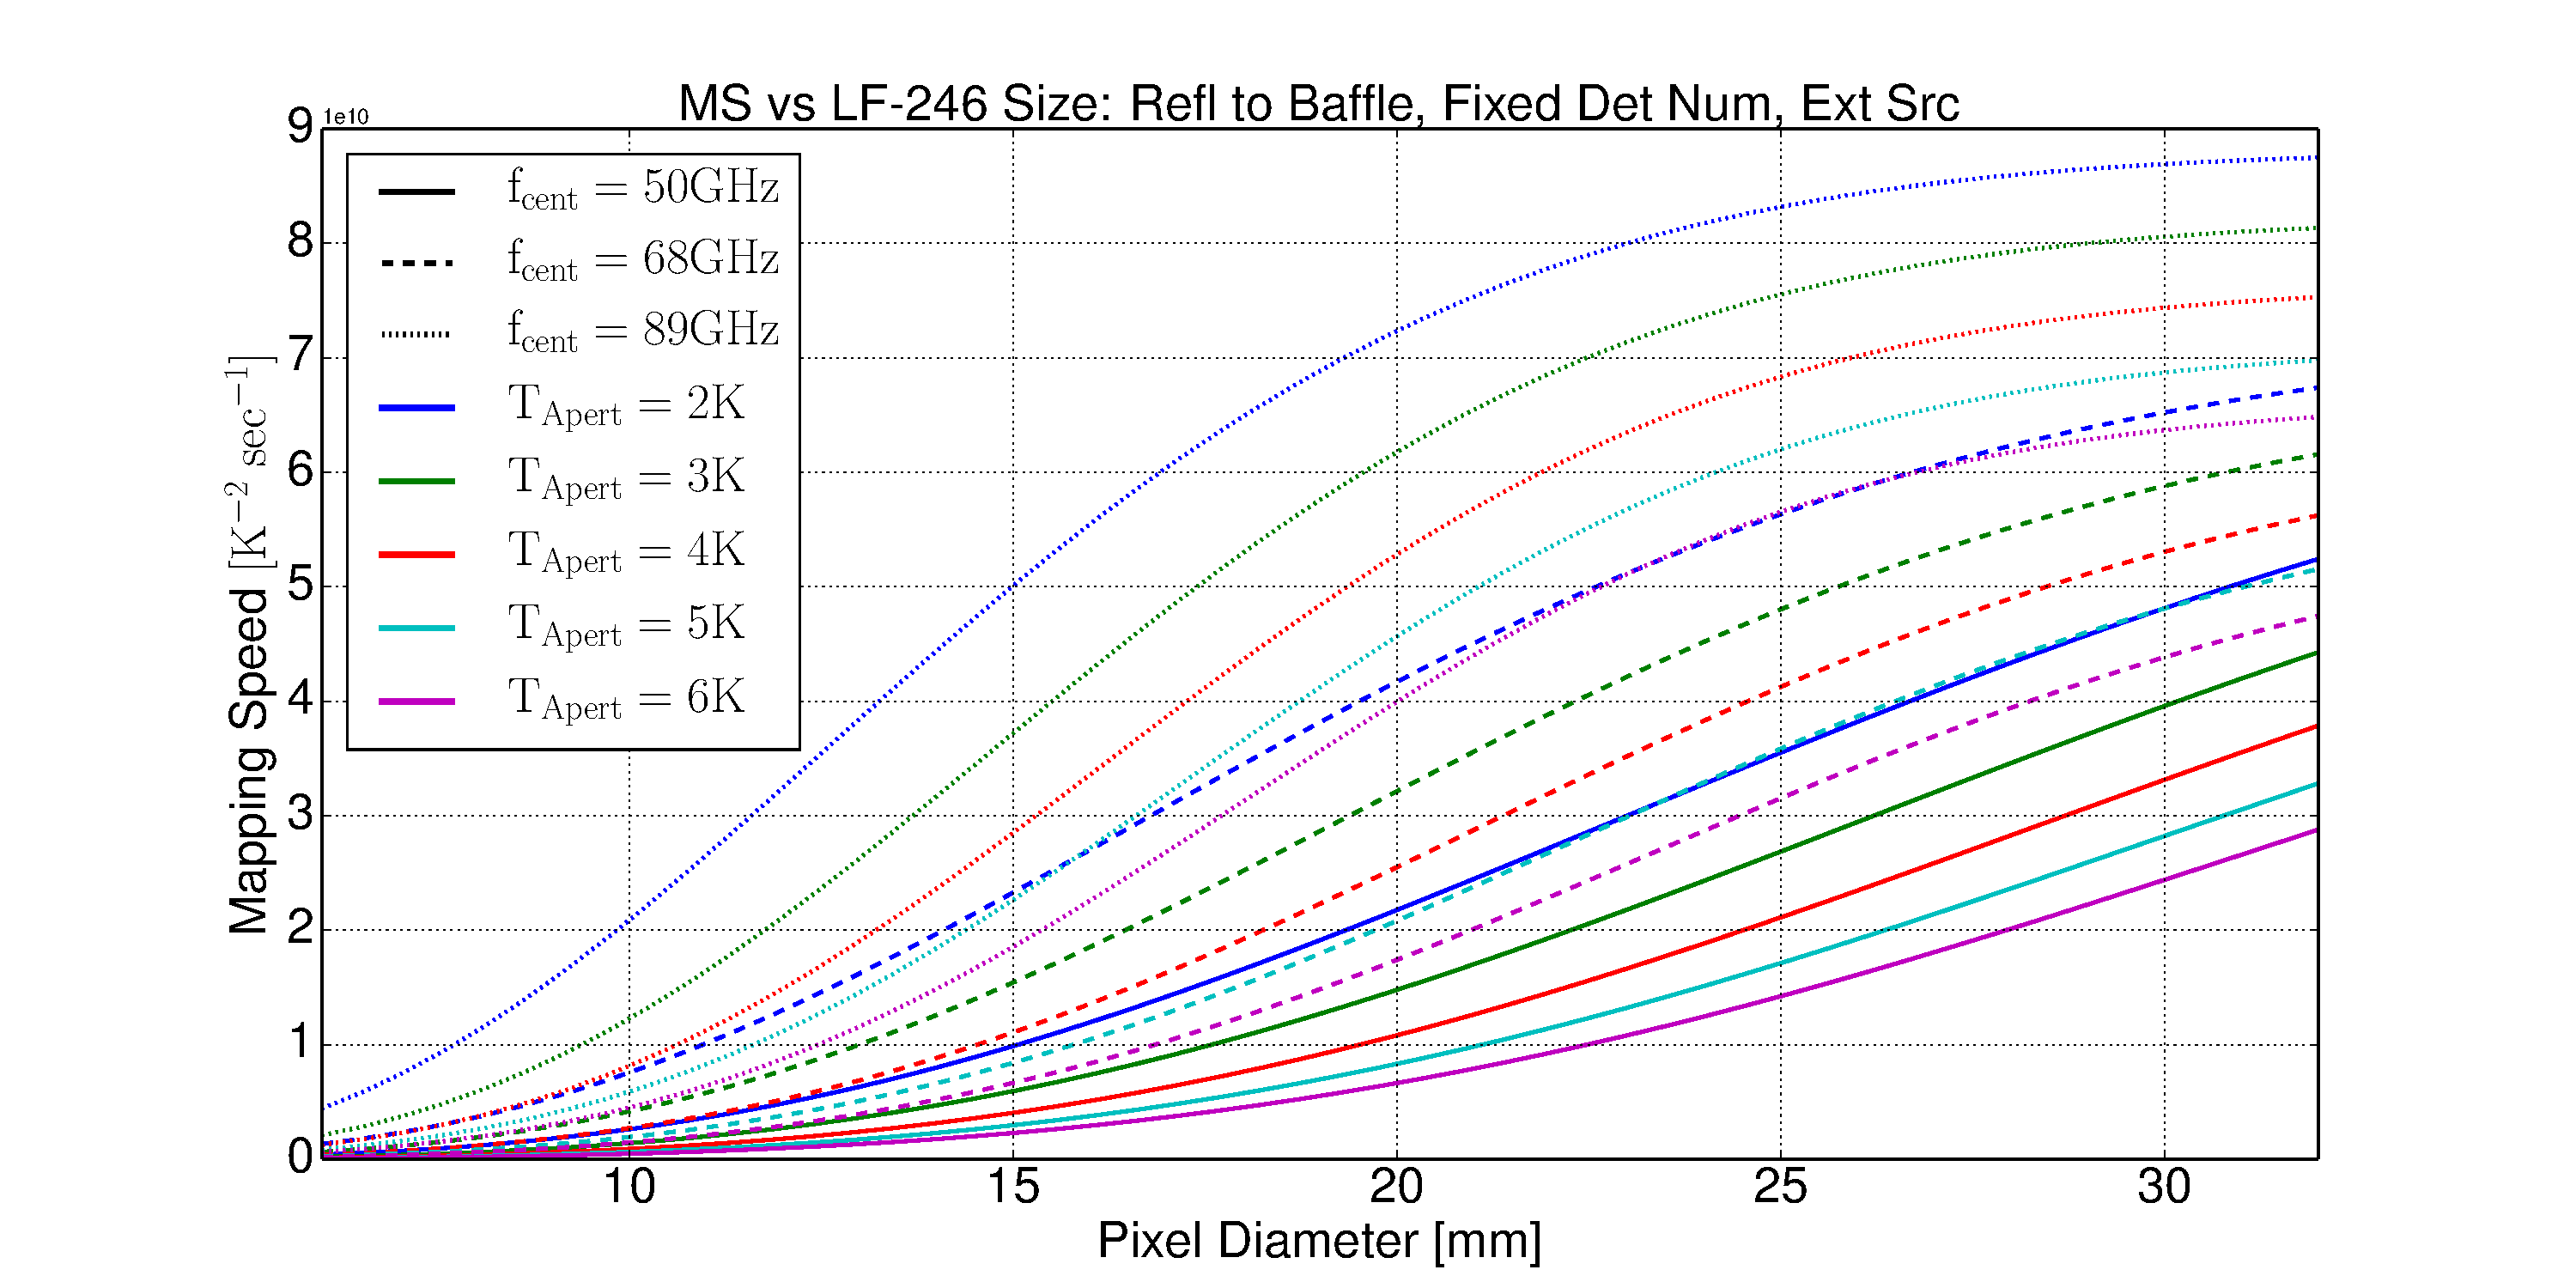
\includegraphics[width=1.1\textwidth, center]{PDF/LFT_MS_LF-246_hotRefl_fixDetNum_extSrc.pdf}
	\caption{LF-246 mapping speed of an extended source as a function of pixel diameter for hot reflections and fixed number of detectors}
\end{figure}

\begin{figure}[H]
	\centering
	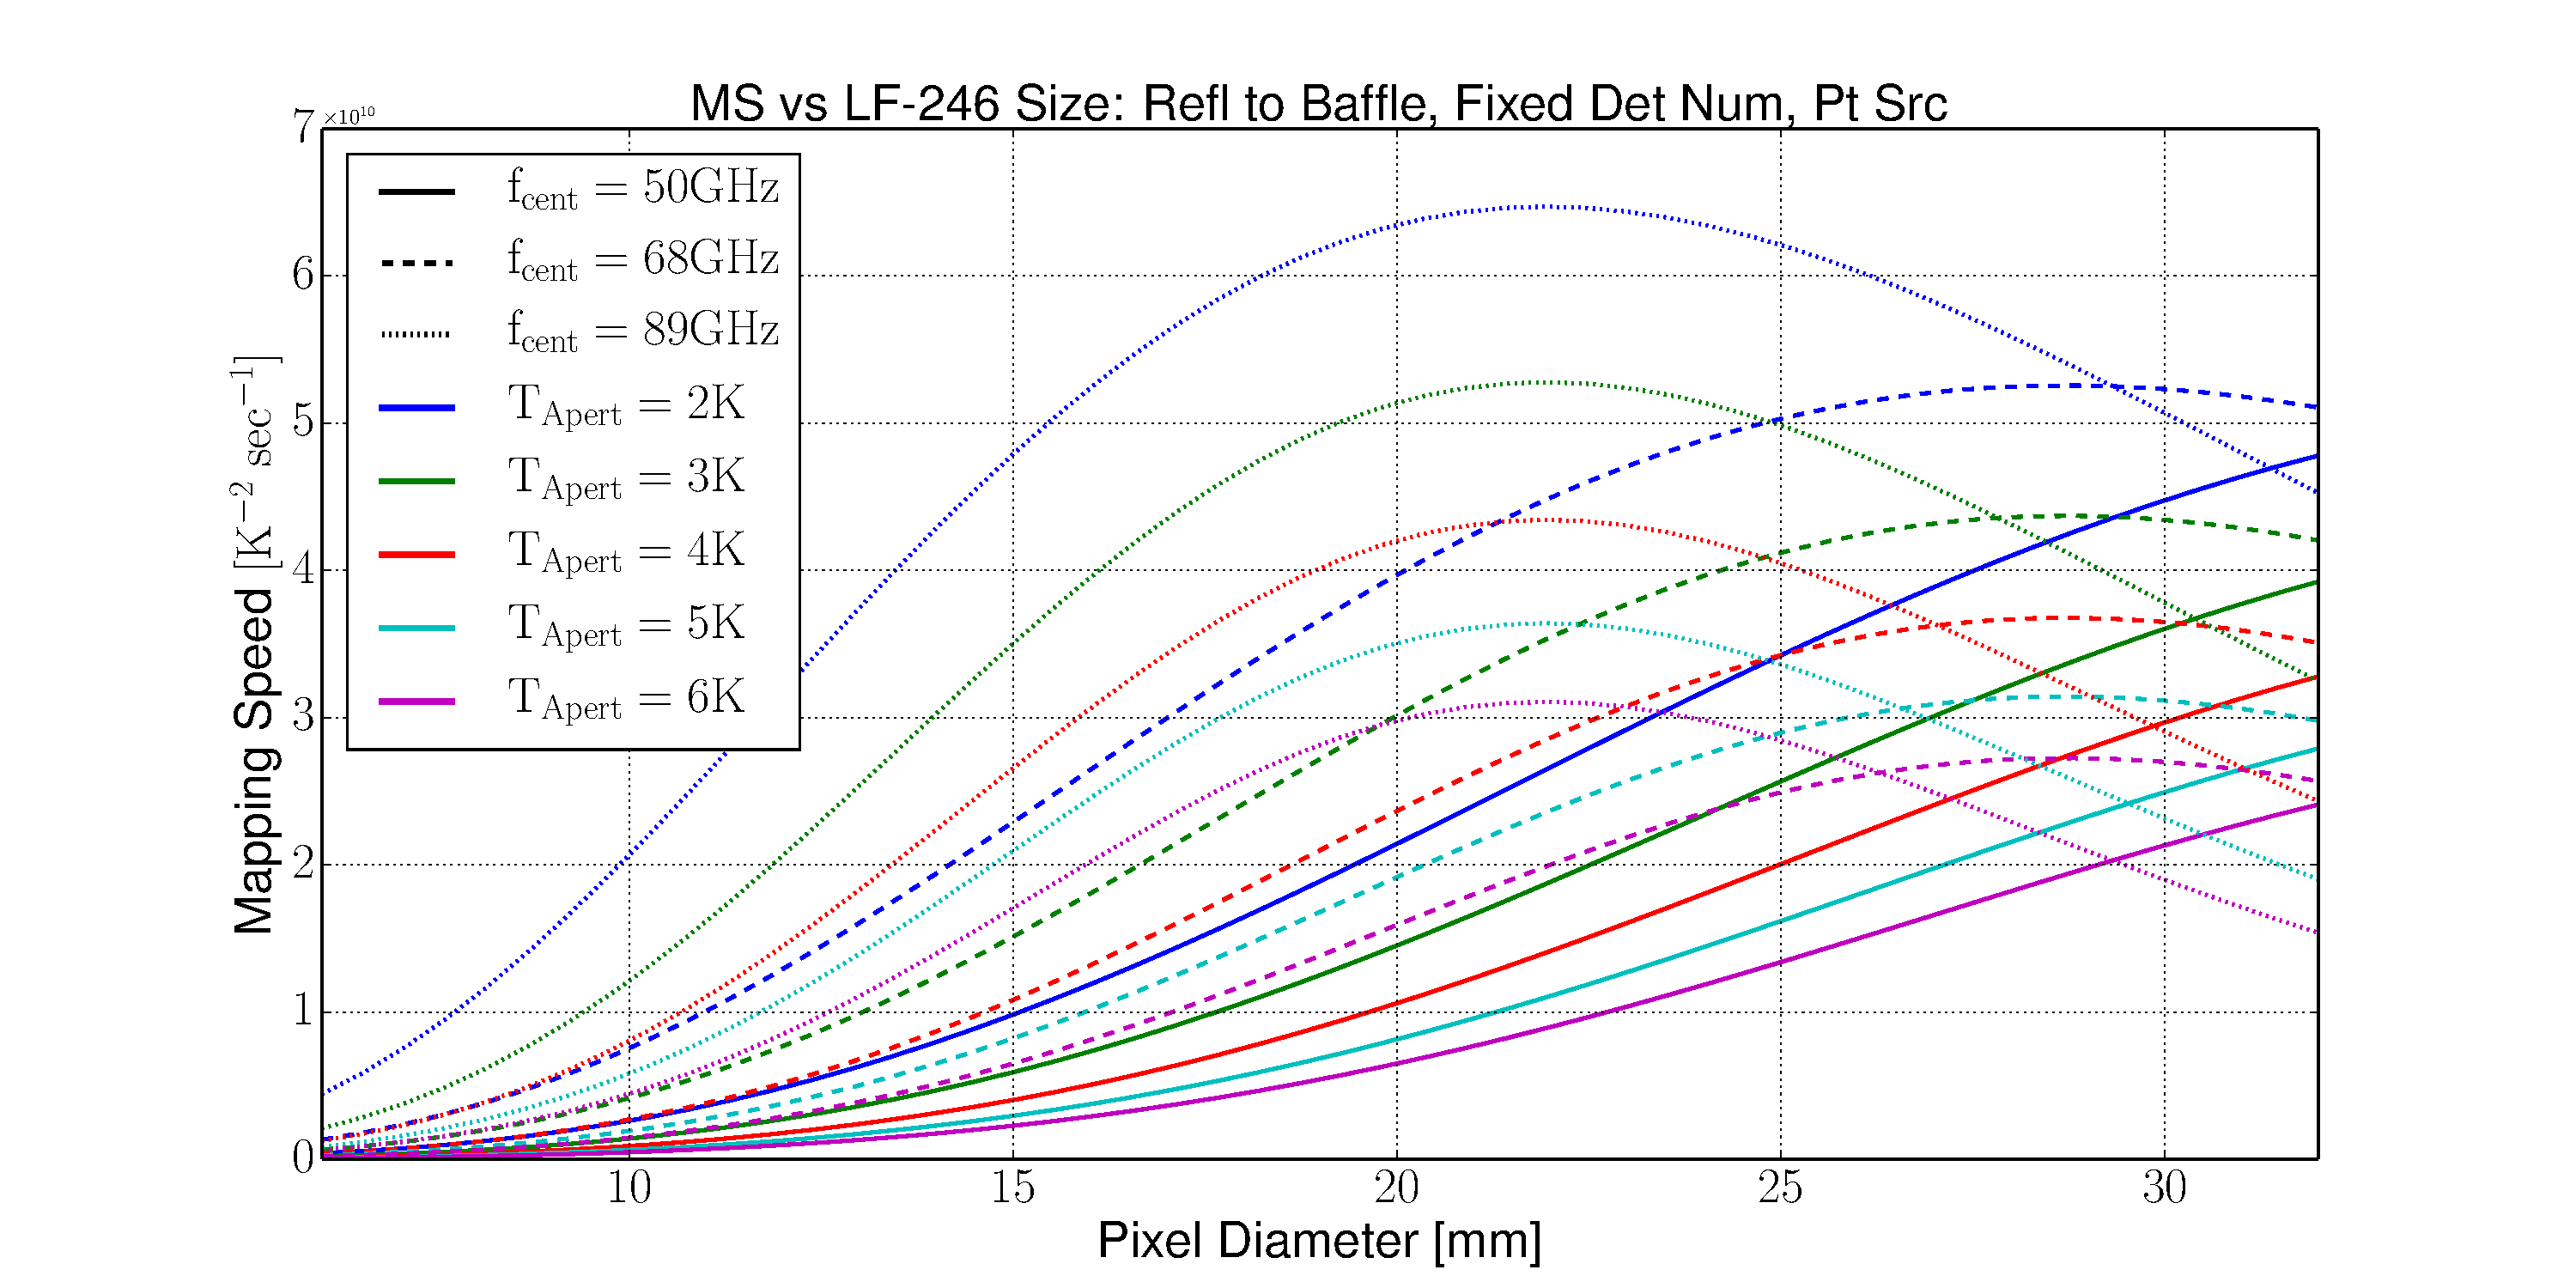
\includegraphics[width=1.1\textwidth, center]{PDF/LFT_MS_LF-246_hotRefl_fixDetNum_ptSrc.pdf}
	\caption{LF-246 mapping speed of a point source as a function of pixel diameter for hot reflections and fixed number of detectors}
\end{figure}

%%%%%%%%%%%%%%%%%%%

\subsubsection{MF-135}

\begin{figure}[H]
	\centering
	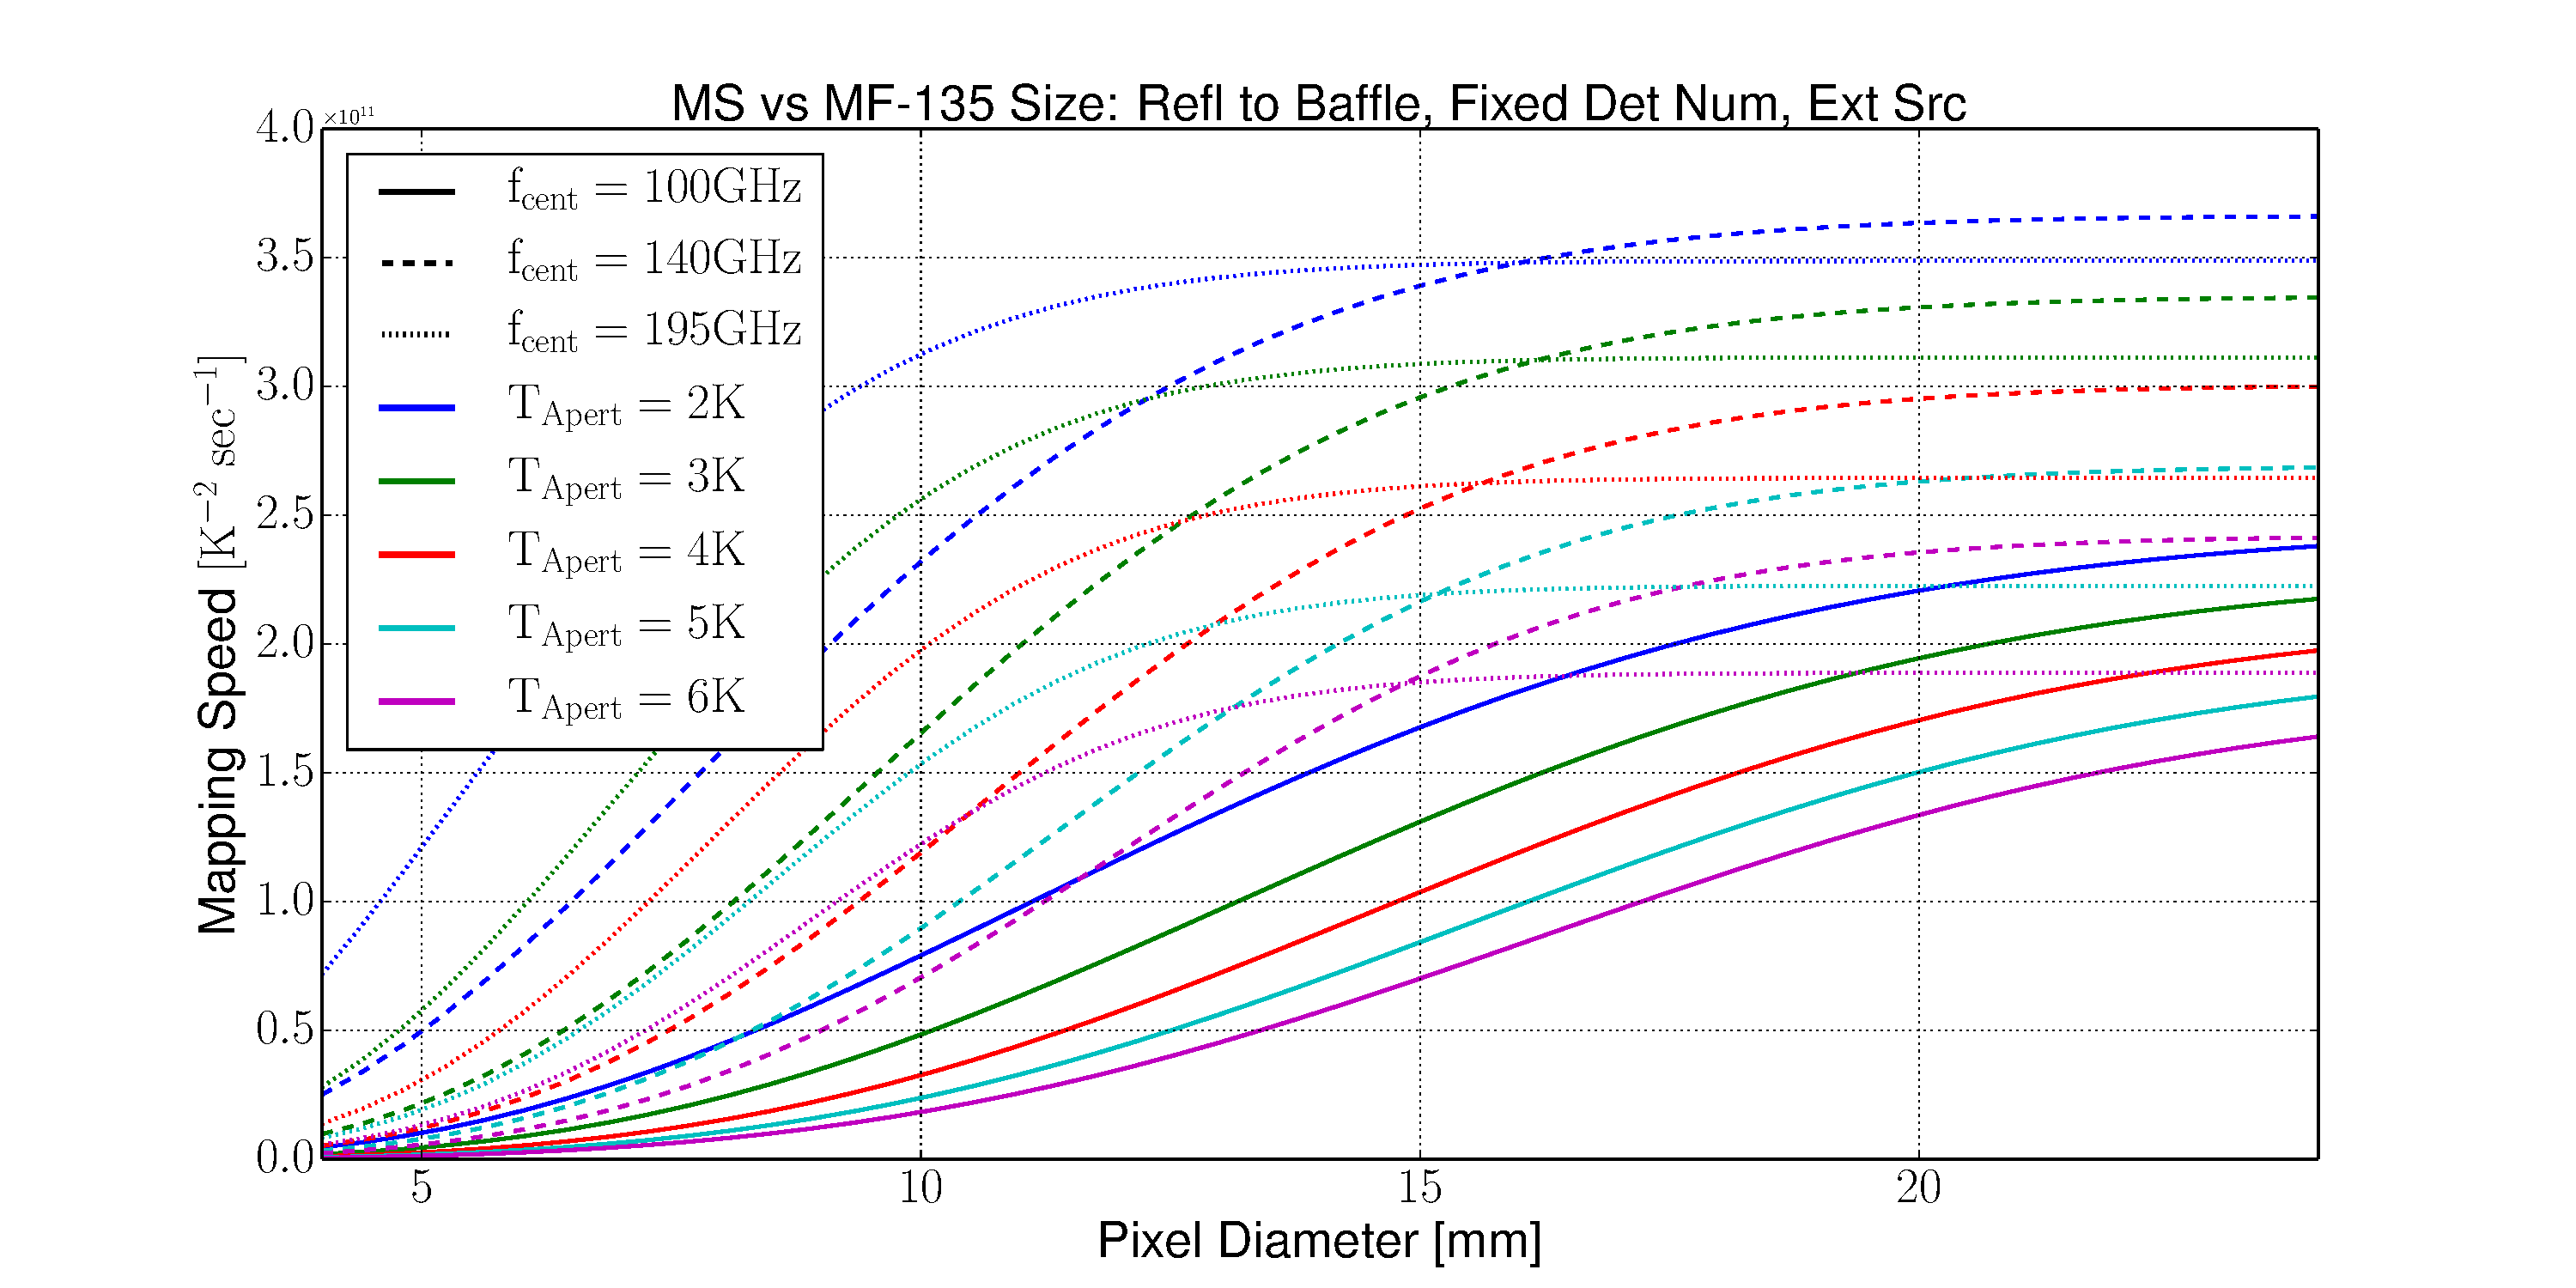
\includegraphics[width=1.1\textwidth, center]{PDF/LFT_MS_MF-135_hotRefl_fixDetNum_extSrc.pdf}
	\caption{MF-135 mapping speed of an extended source as a function of pixel diameter for hot reflections and fixed number of detectors}
\end{figure}

\begin{figure}[H]
	\centering
	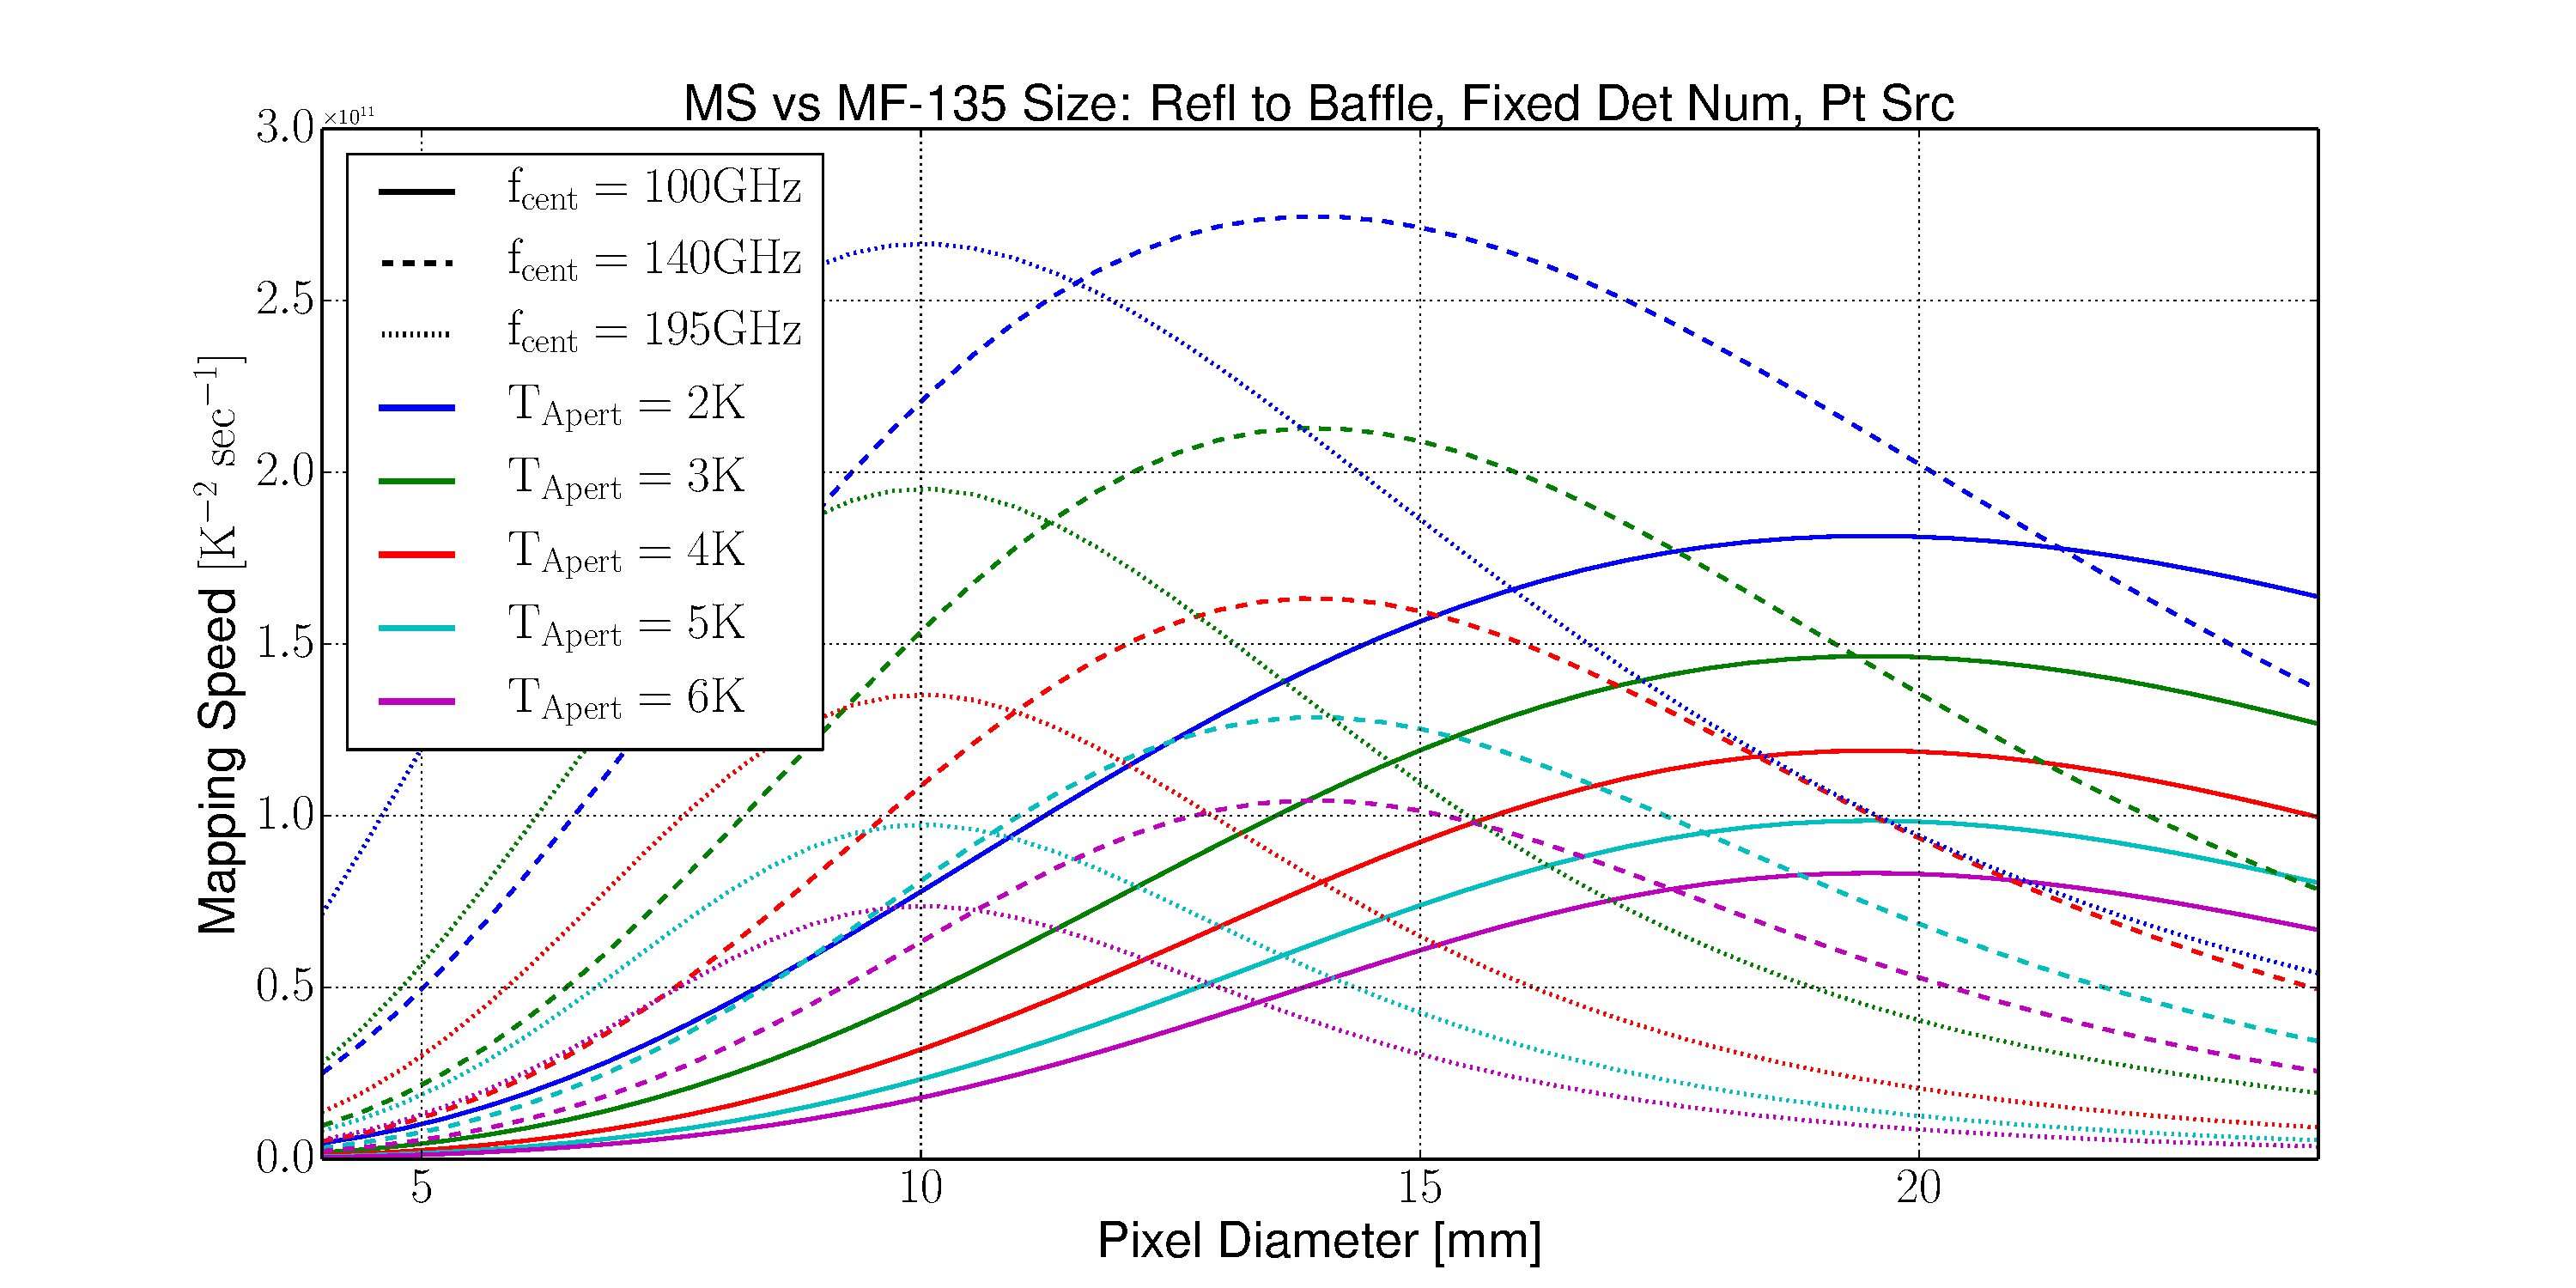
\includegraphics[width=1.1\textwidth, center]{PDF/LFT_MS_MF-135_hotRefl_fixDetNum_ptSrc.pdf}
	\caption{MF-135 mapping speed of a point source as a function of pixel diameter for hot reflections and fixed number of detectors}
\end{figure}

%%%%%%%%%%%%%%%%%%%

\subsubsection{MF-246}

\begin{figure}[H]
	\centering
	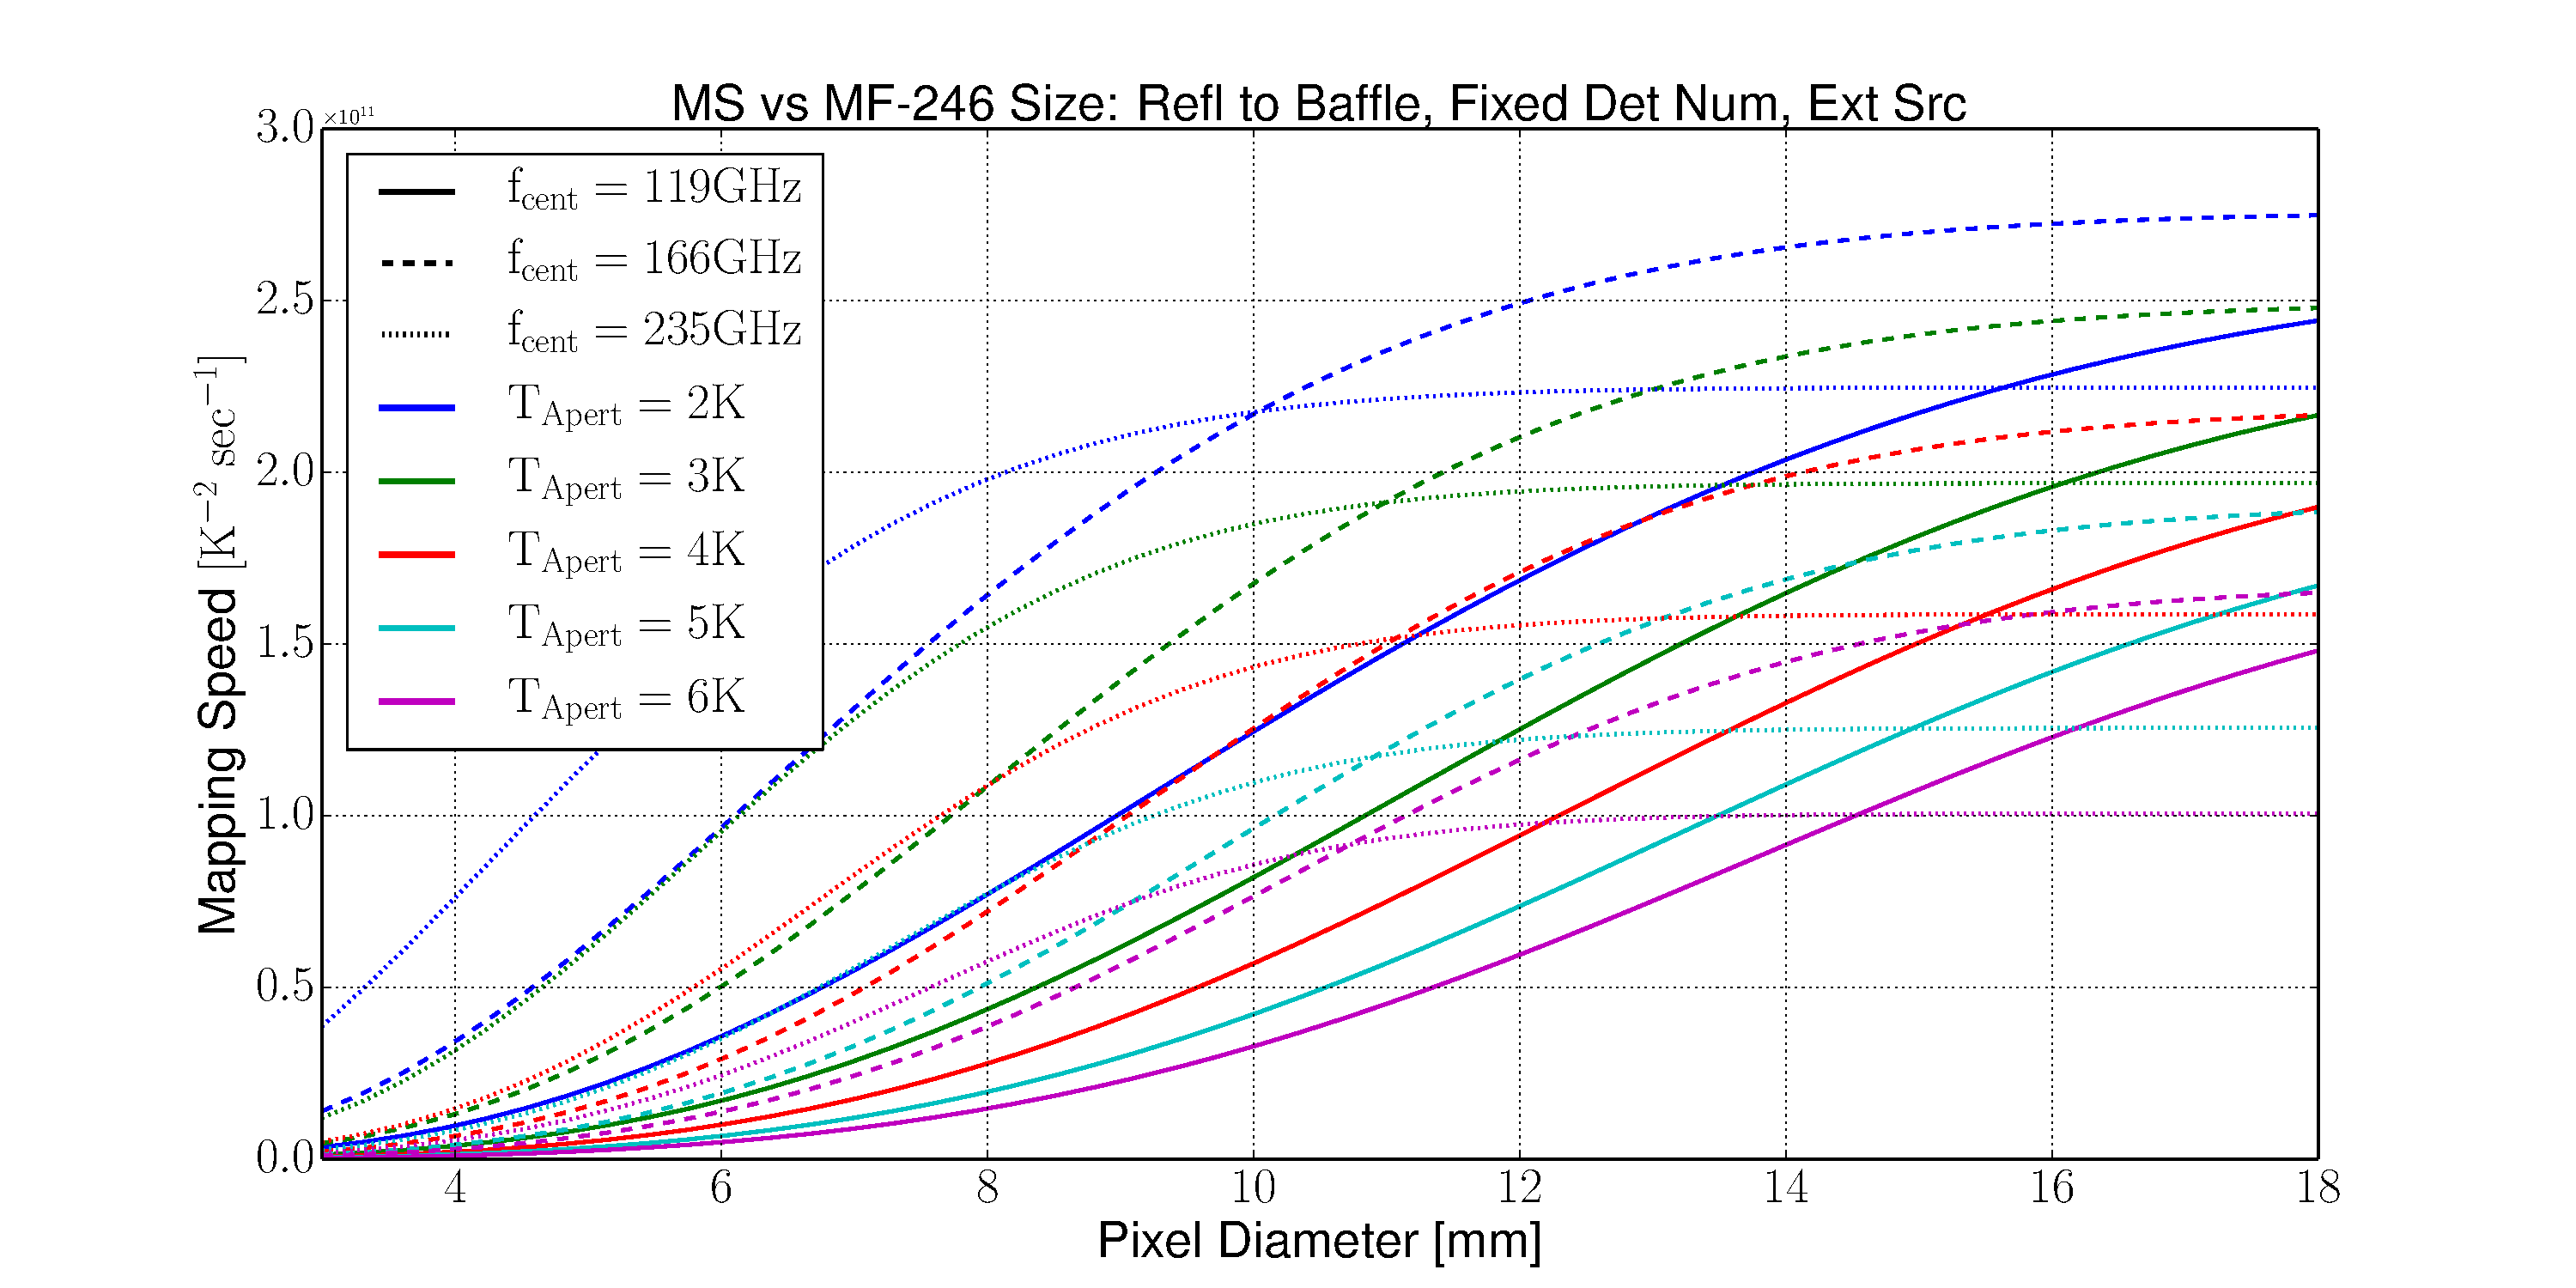
\includegraphics[width=1.1\textwidth, center]{PDF/LFT_MS_MF-246_hotRefl_fixDetNum_extSrc.pdf}
	\caption{MF-246 mapping speed of an extended source as a function of pixel diameter for hot reflections and fixed number of detectors}
\end{figure}

\begin{figure}[H]
	\centering
	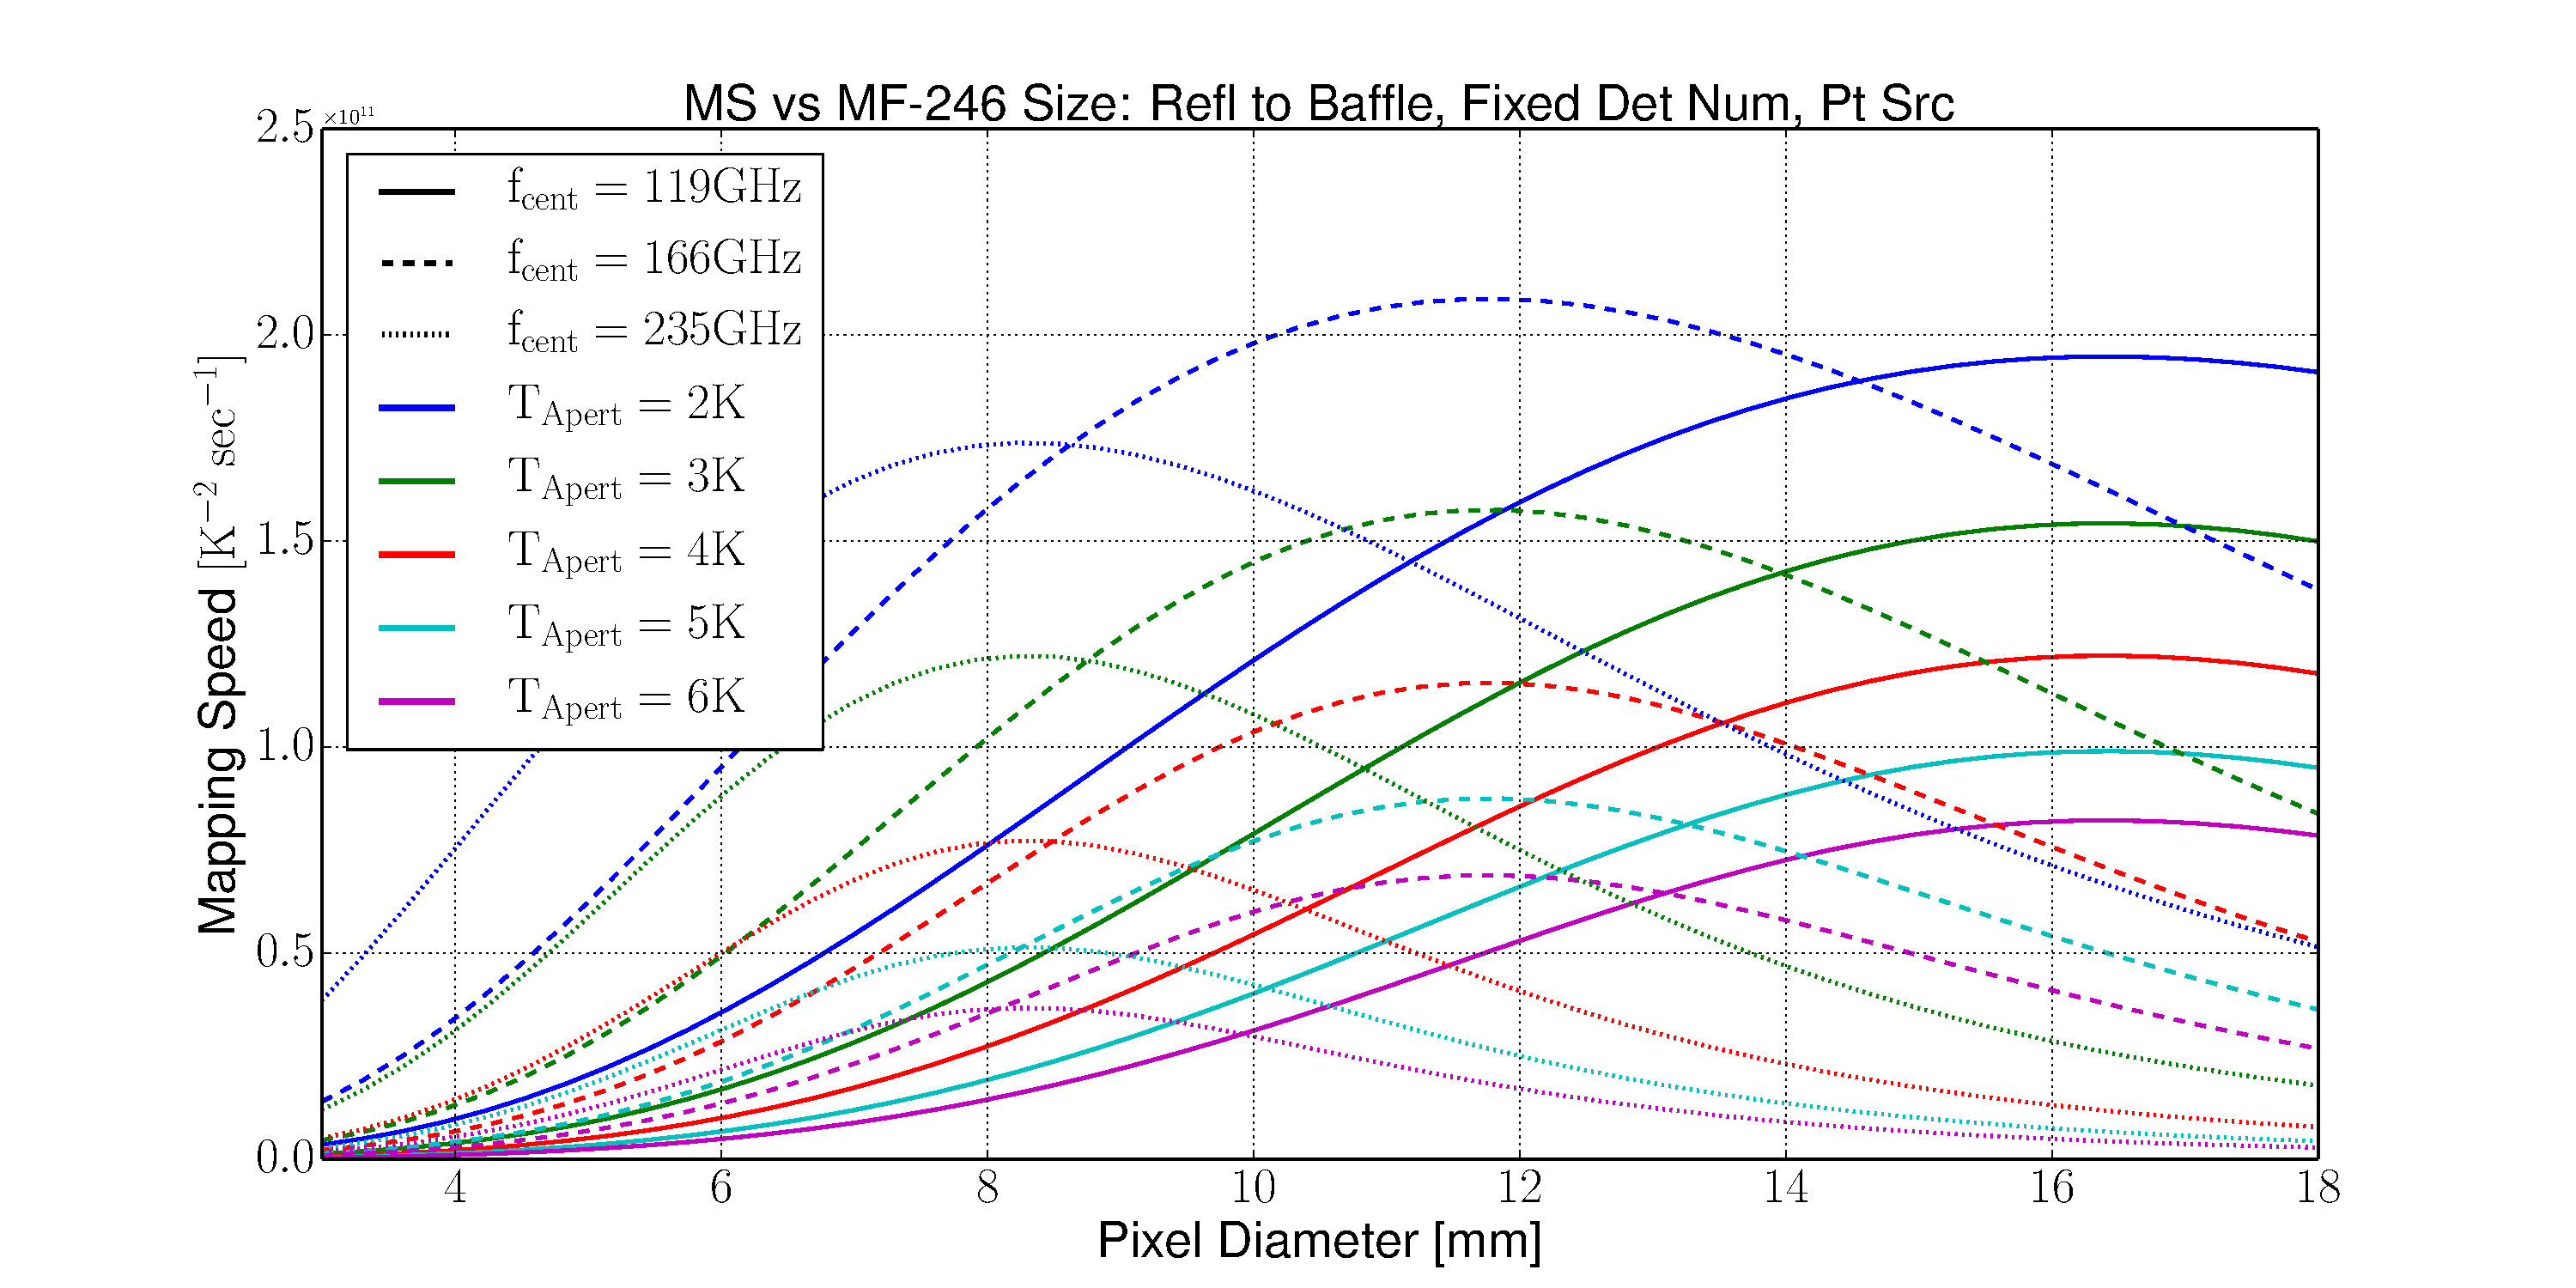
\includegraphics[width=1.1\textwidth, center]{PDF/LFT_MS_MF-246_hotRefl_fixDetNum_ptSrc.pdf}
	\caption{MF-246 mapping speed of a point source as a function of pixel diameter for hot reflections and fixed number of detectors}
\end{figure}

%%%%%%%%%%%%%%%%%%%

\subsubsection{HFT}

\begin{figure}[H]
	\centering
	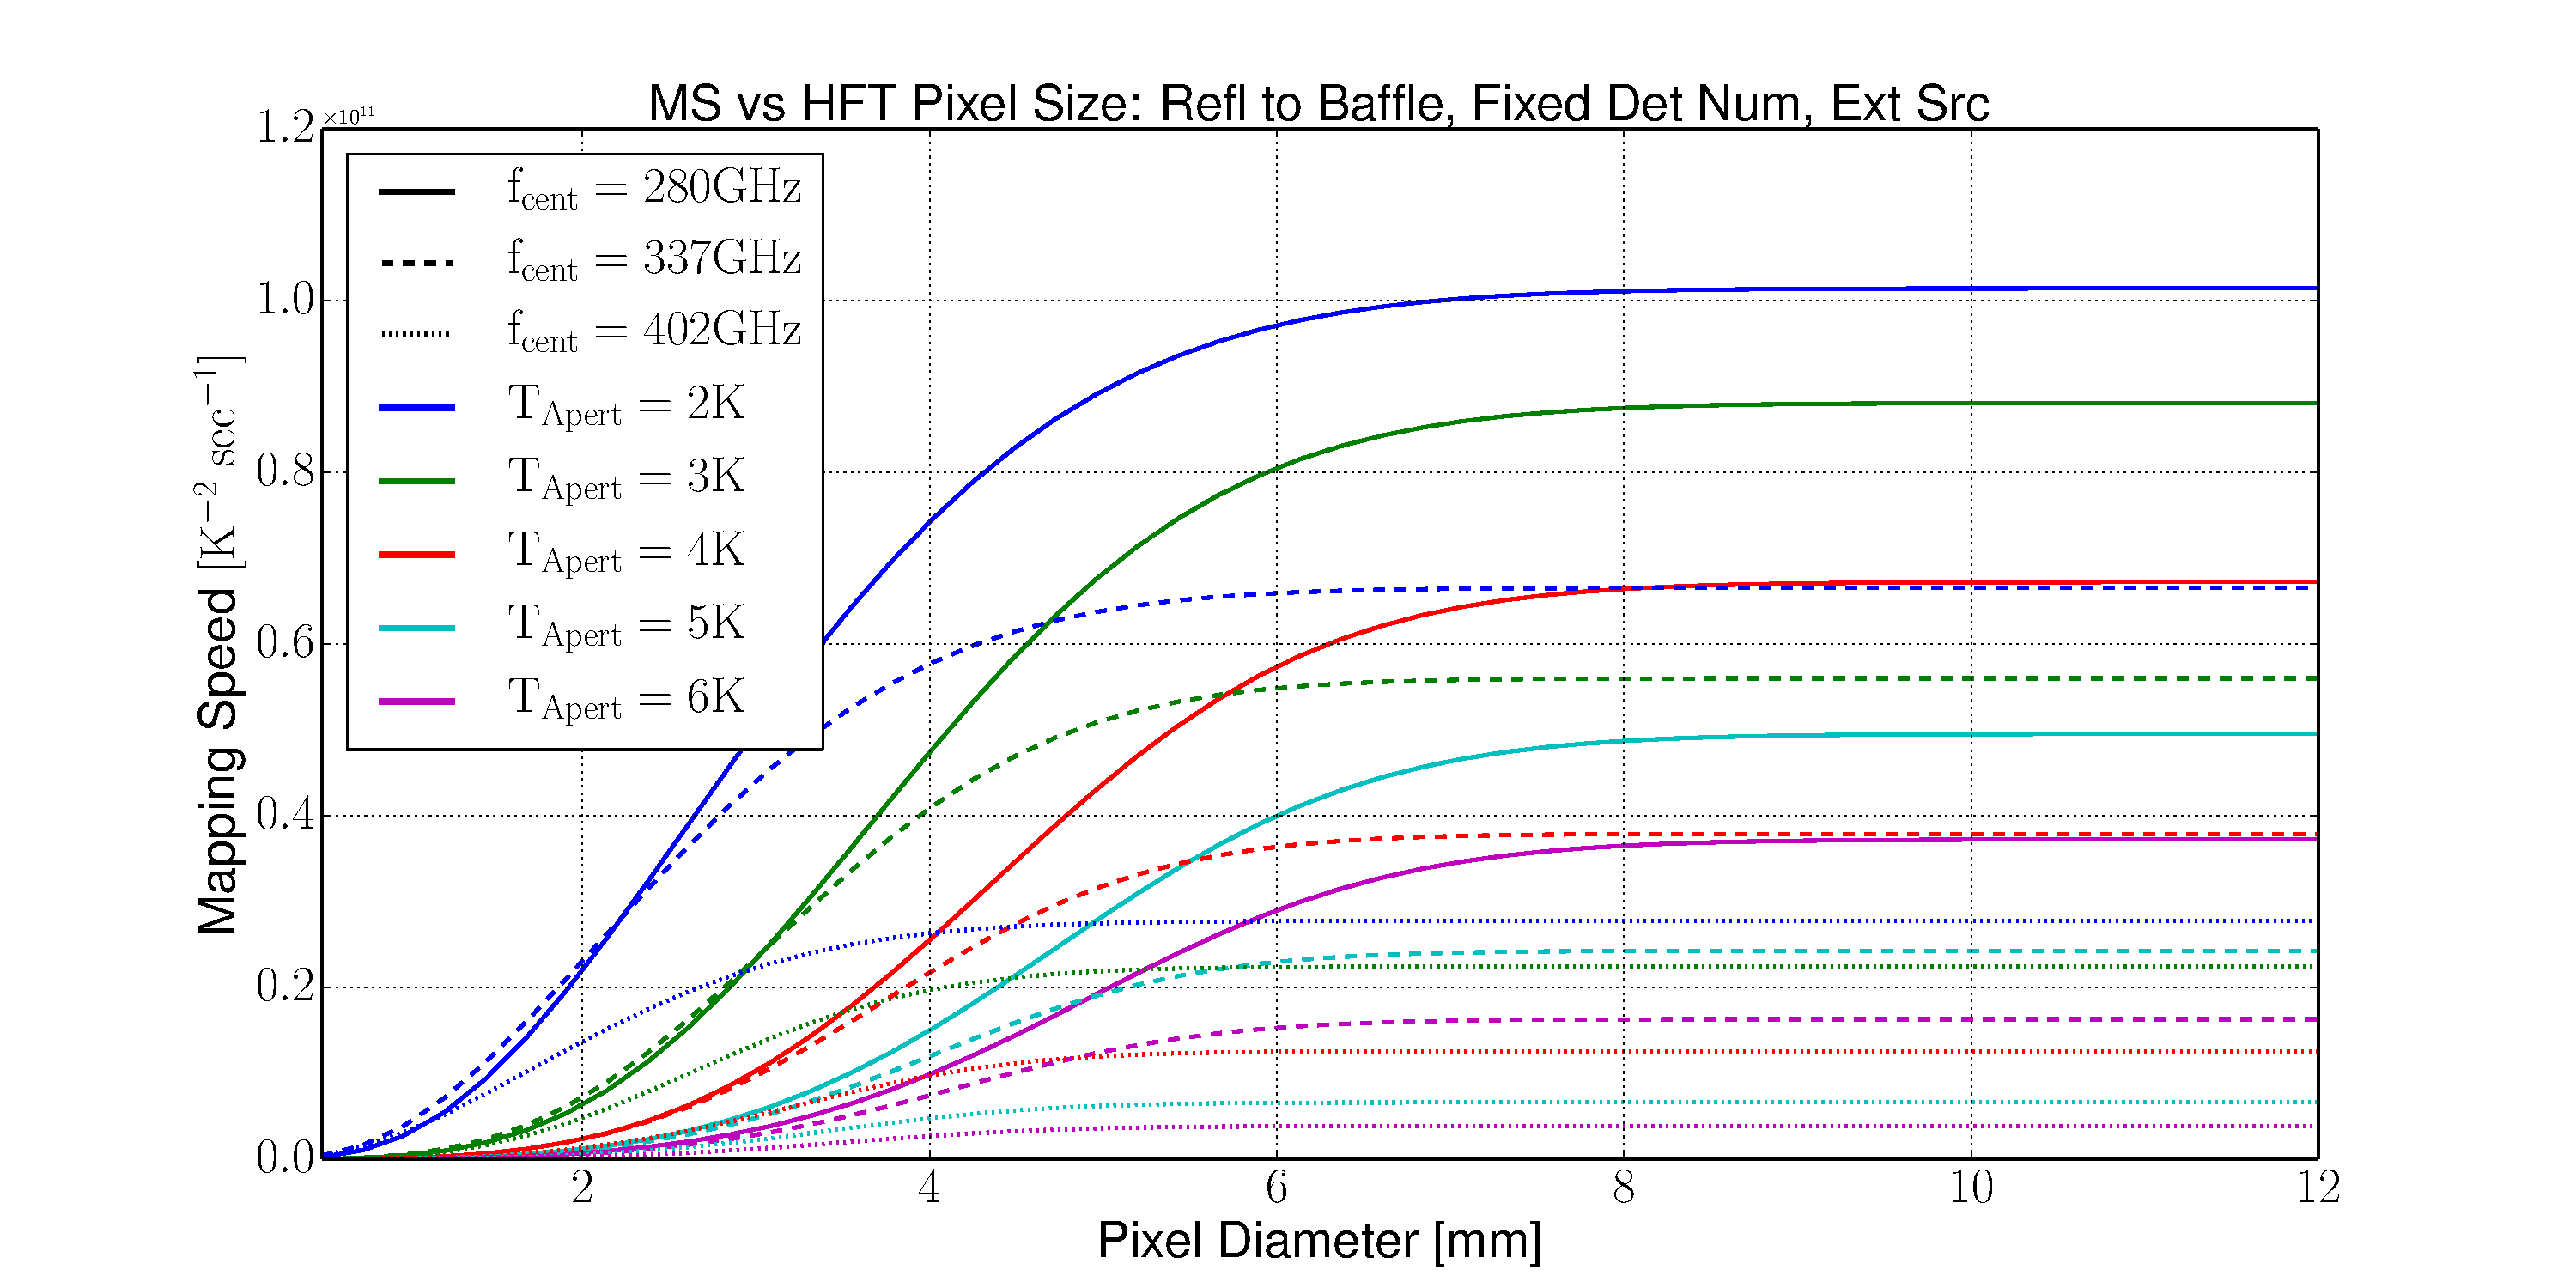
\includegraphics[width=1.1\textwidth, center]{PDF/HFT_MS_hotRefl_fixDetNum_extSrc.pdf}
	\caption{HFT mapping speed of an extended source as a function of pixel diameter for hot reflections and fixed number of detectors}
\end{figure}

\begin{figure}[H]
	\centering
	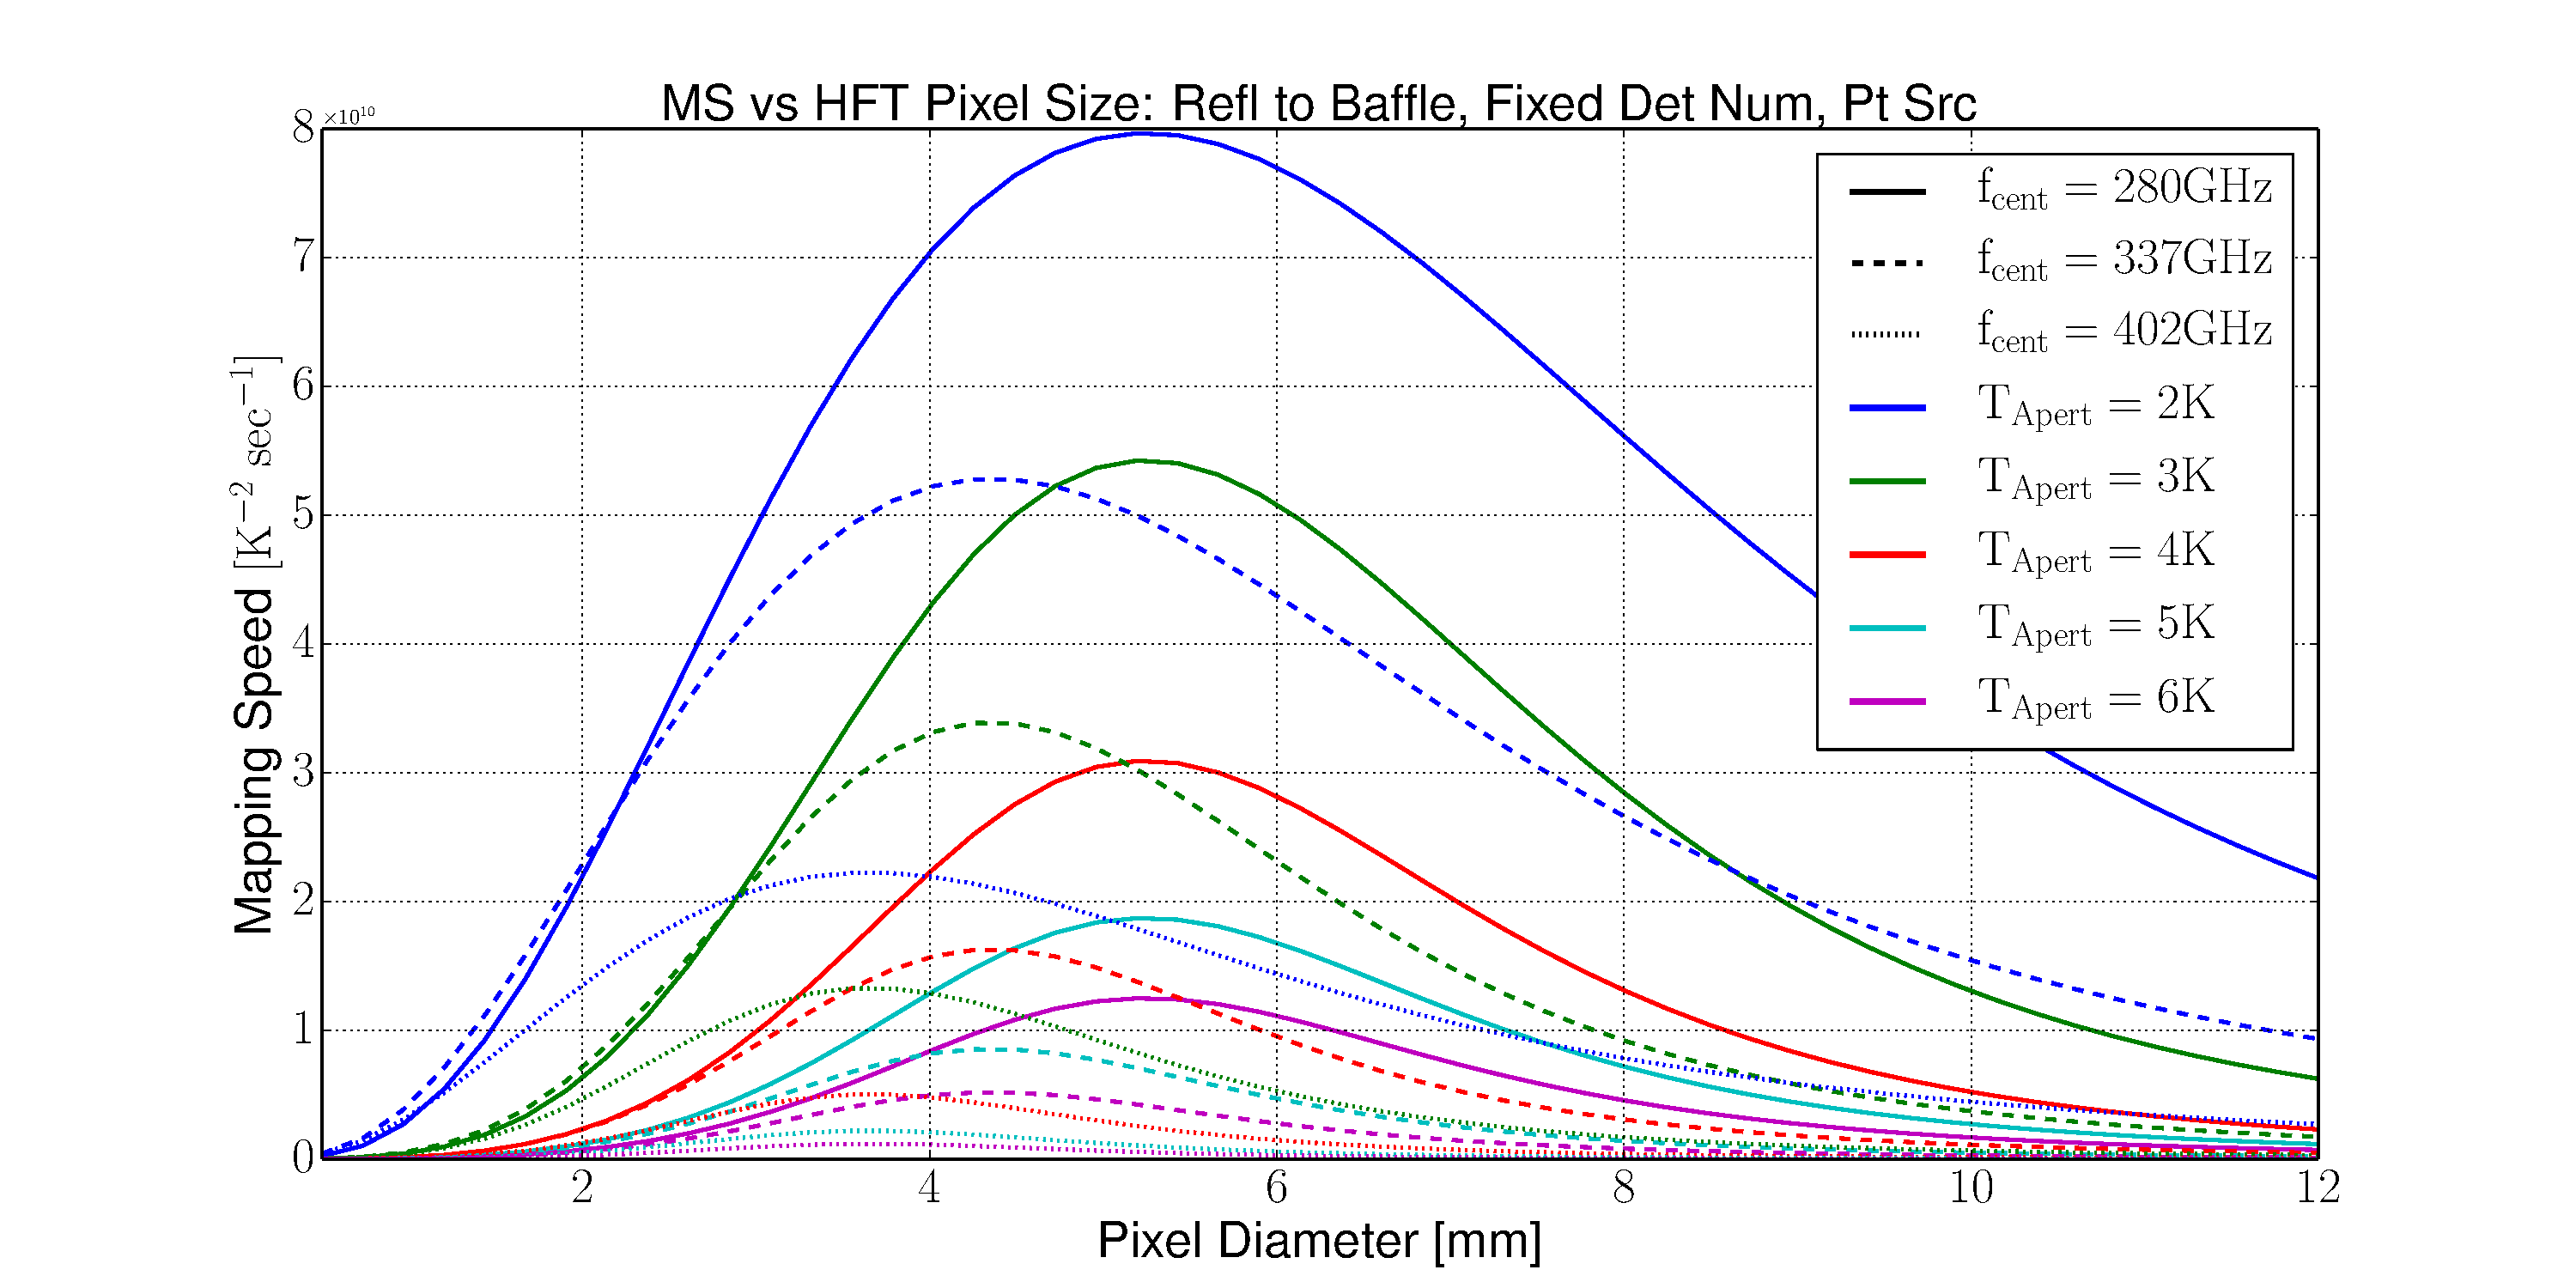
\includegraphics[width=1.1\textwidth, center]{PDF/HFT_MS_hotRefl_fixDetNum_ptSrc.pdf}
	\caption{HFT mapping speed of a point source as a function of pixel diameter for hot reflections and fixed number of detectors}
\end{figure}

%%%%%%%%%%%%%%%%%%%%%%%%%%%%%%%%%%%%%

\subsection{Reflections Go to Focal Plane, Fixed FOV}

This subsection containts the results for the optimization of pixel diameters for the LFT and HFT given a fixed field of view and assuming all reflections go back to the focal plane.

\clearpage

%%%%%%%%%%%%%%%%%%%

\subsubsection{LF-135}

\begin{figure}[H]
	\centering
	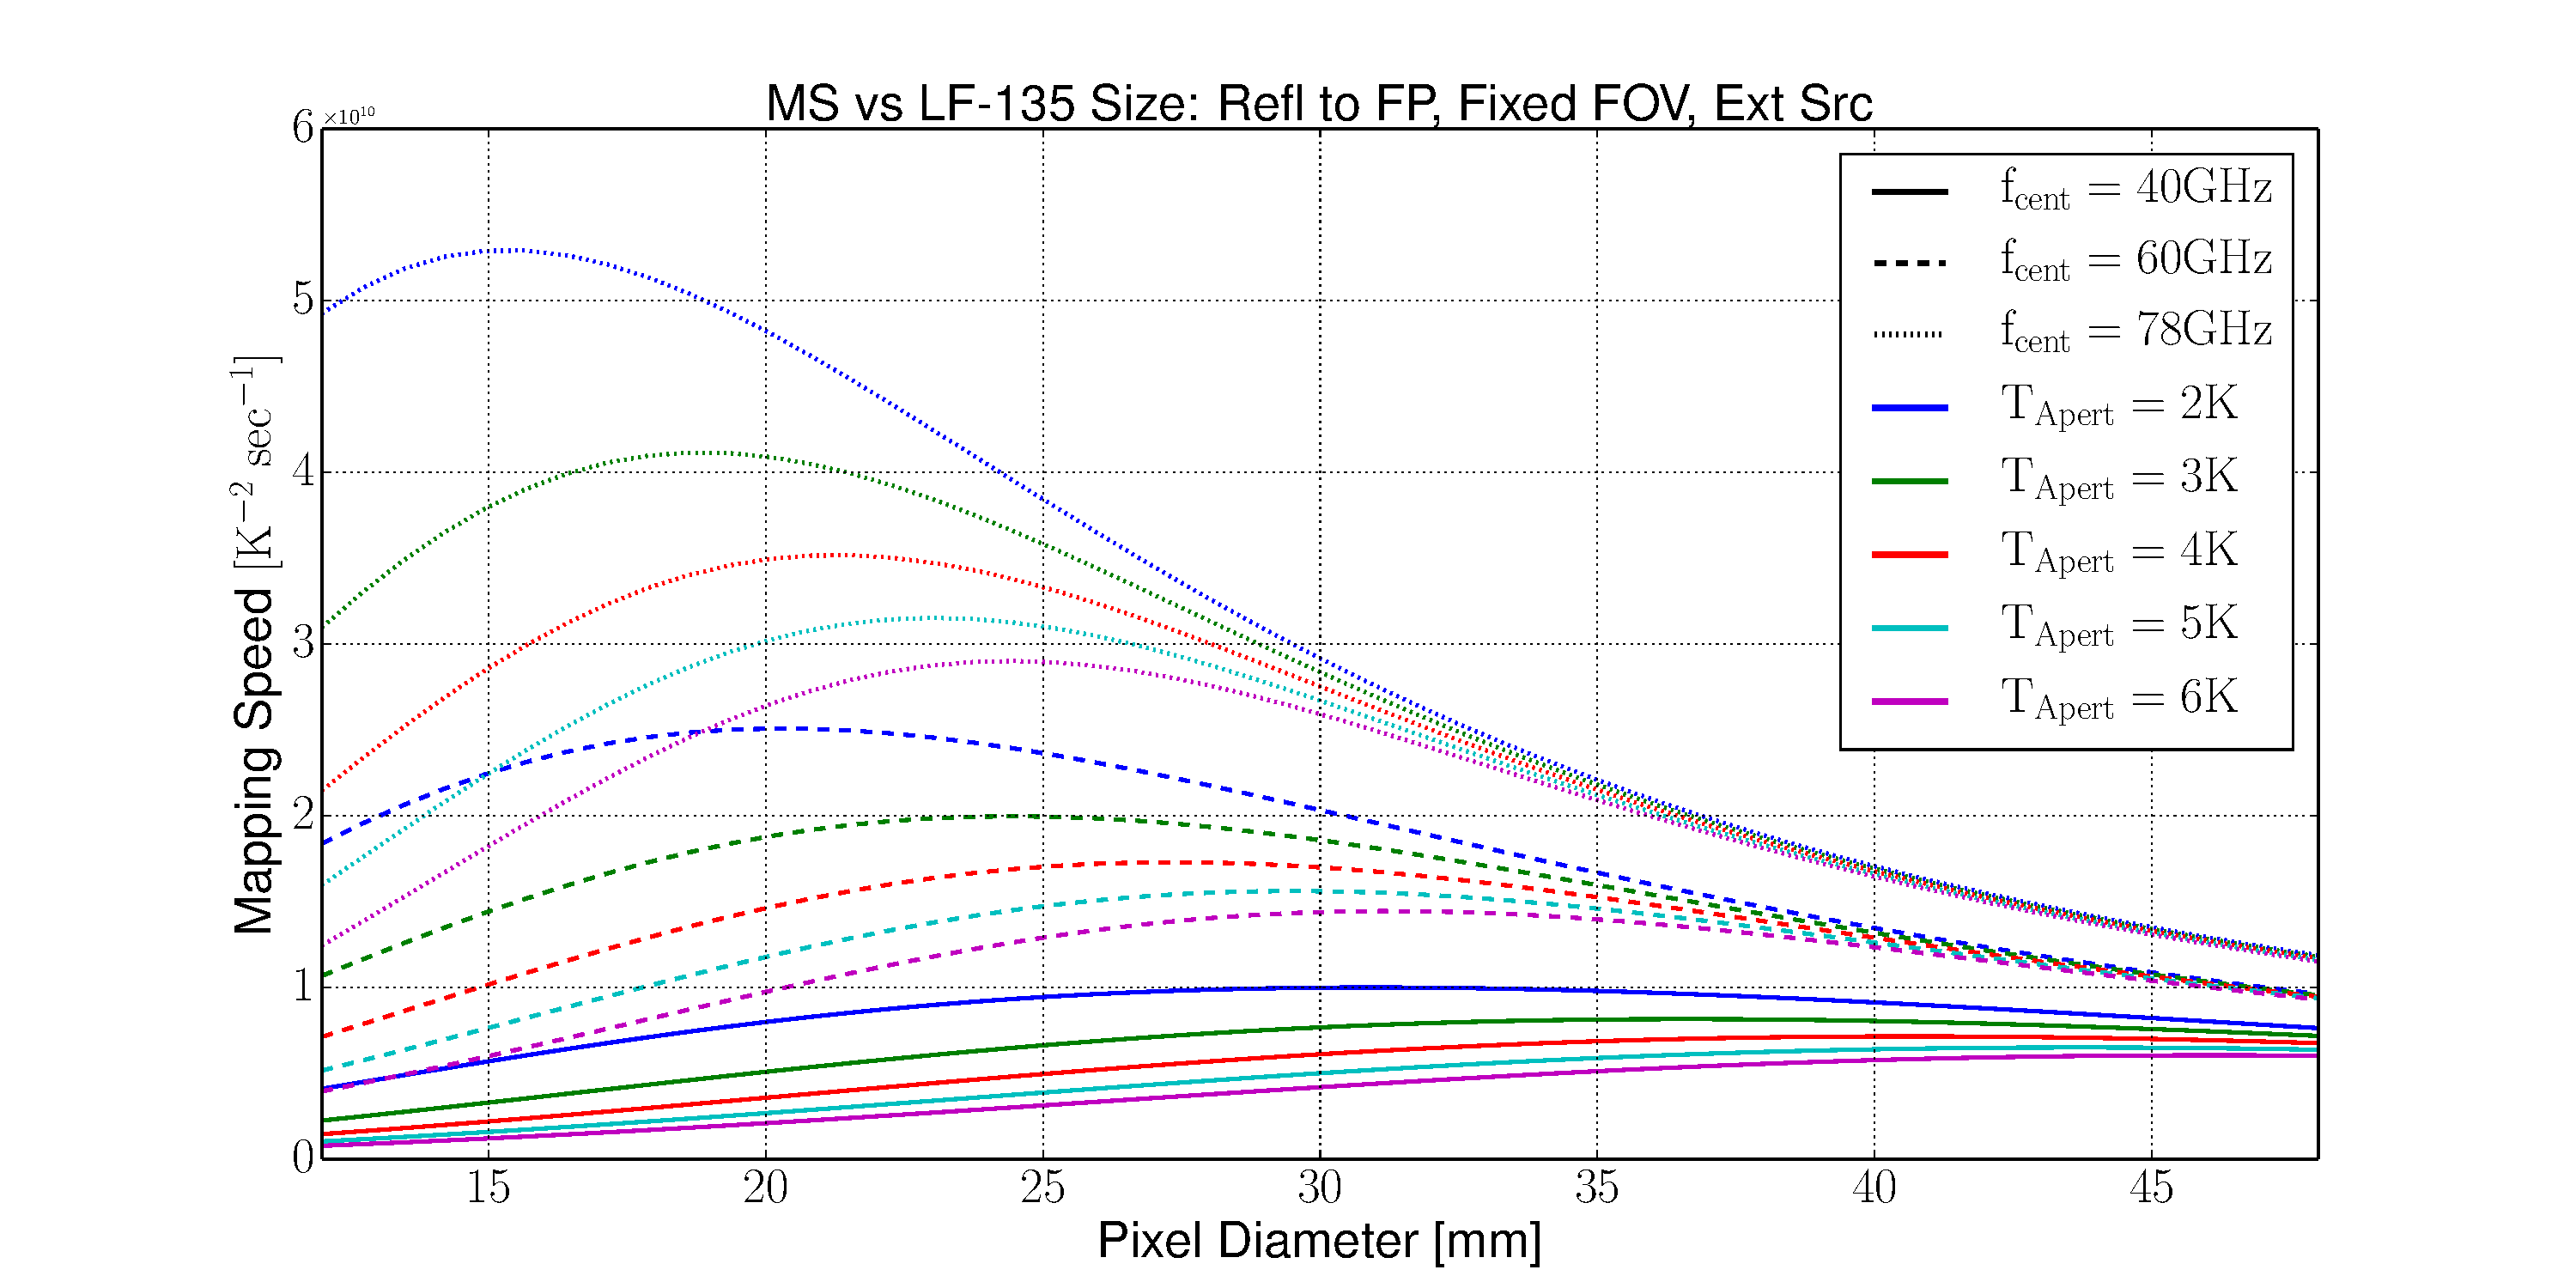
\includegraphics[width=1.1\textwidth, center]{PDF/LFT_MS_LF-135_coldRefl_fixFOV_extSrc.pdf}
	\caption{LF-135 mapping speed of an extended source as a function of pixel diameter for cold reflections and fixed FOV}
\end{figure}

\begin{figure}[H]
	\centering
	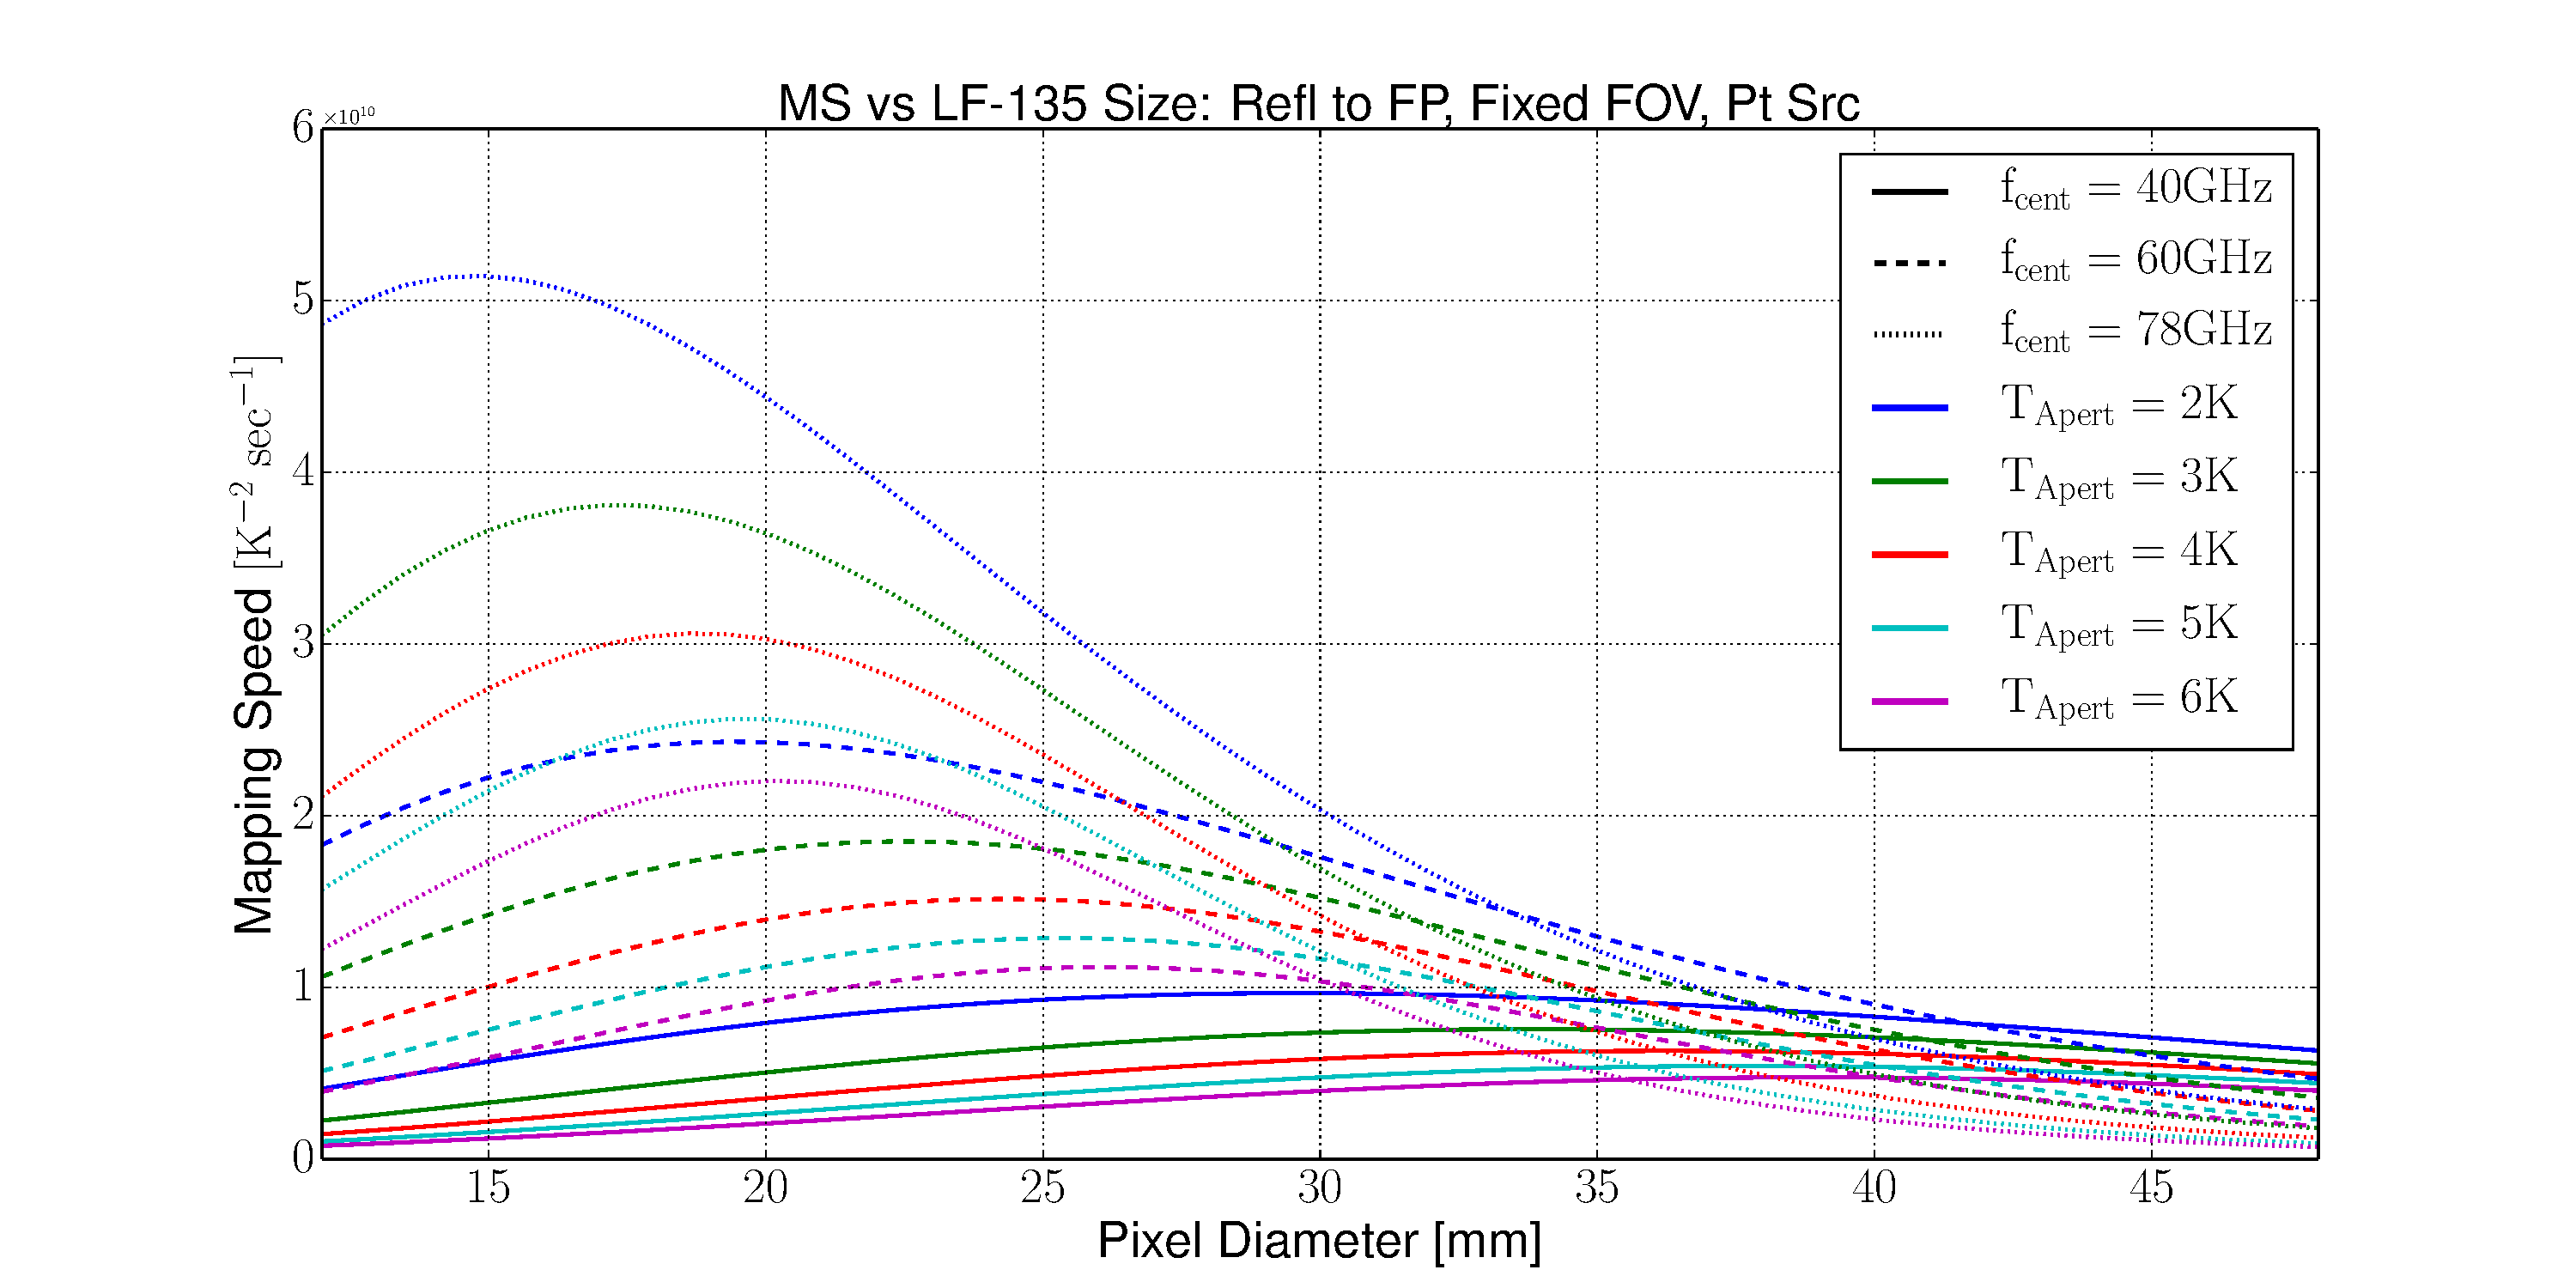
\includegraphics[width=1.1\textwidth, center]{PDF/LFT_MS_LF-135_coldRefl_fixFOV_ptSrc.pdf}
	\caption{LF-135 mapping speed of a point source as a function of pixel diameter for cold reflections and fixed FOV}
\end{figure}

%%%%%%%%%%%%%%%%%%%

\subsubsection{LF-246}

\begin{figure}[H]
	\centering
	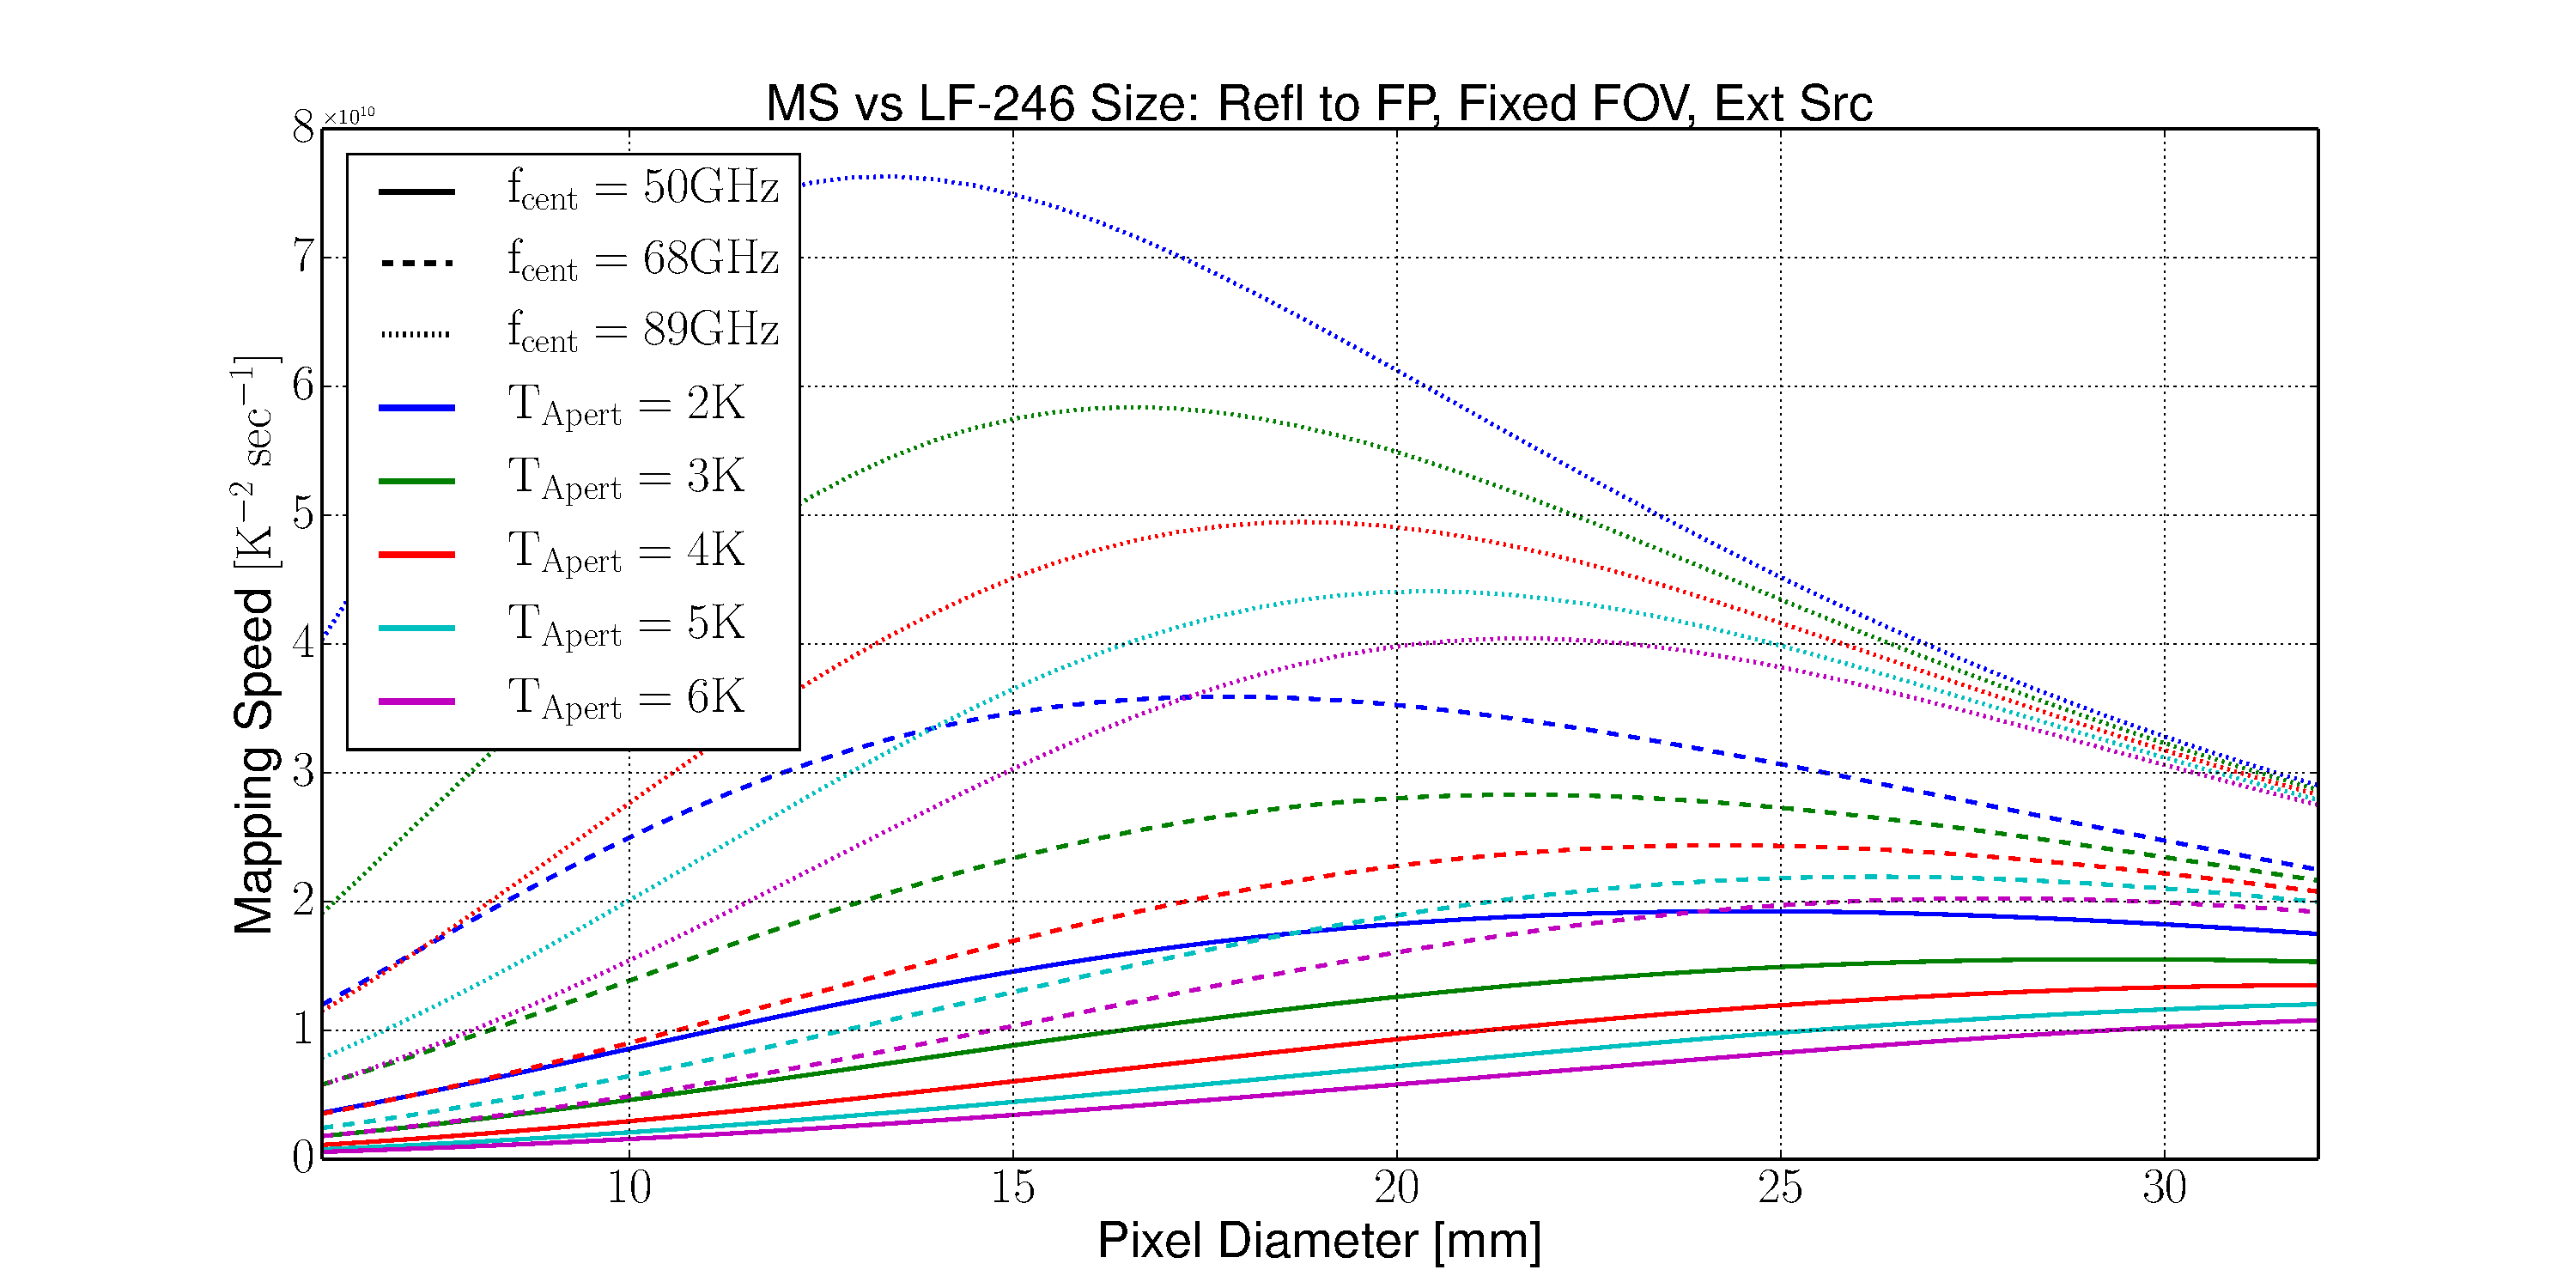
\includegraphics[width=1.1\textwidth, center]{PDF/LFT_MS_LF-246_coldRefl_fixFOV_extSrc.pdf}
	\caption{LF-246 mapping speed of an extended source as a function of pixel diameter for cold reflections and fixed FOV}
\end{figure}

\begin{figure}[H]
	\centering
	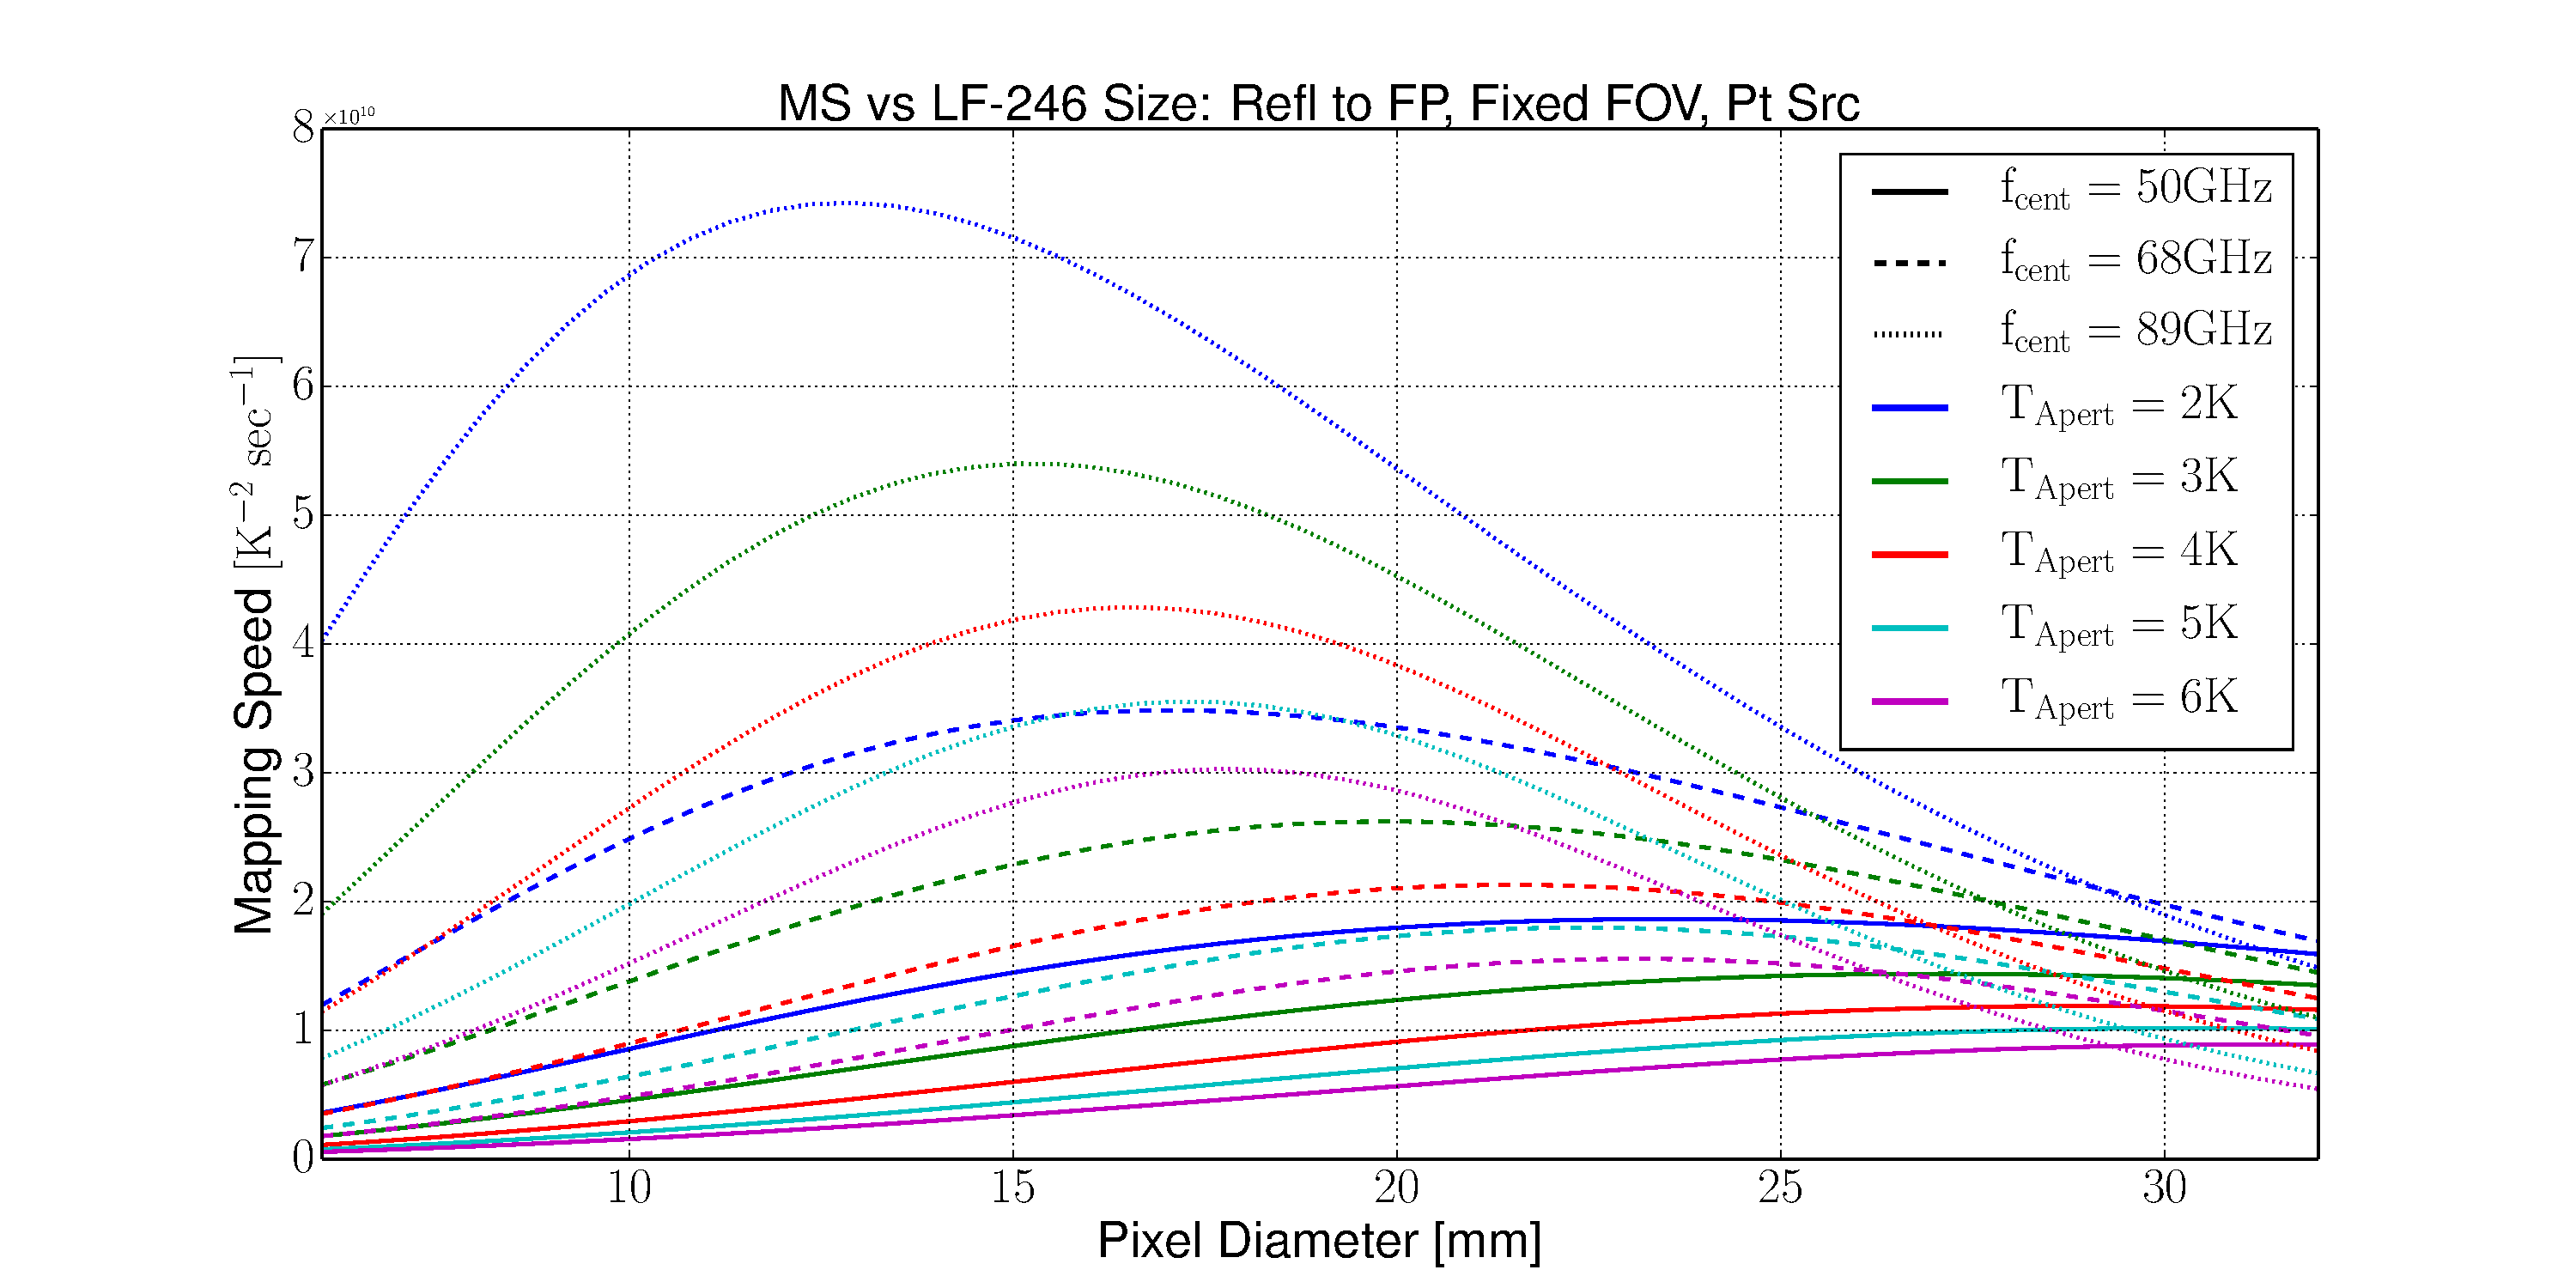
\includegraphics[width=1.1\textwidth, center]{PDF/LFT_MS_LF-246_coldRefl_fixFOV_ptSrc.pdf}
	\caption{LF-246 mapping speed of a point source as a function of pixel diameter for cold reflections and fixed FOV}
\end{figure}

%%%%%%%%%%%%%%%%%%%

\subsubsection{MF-135 Pixel}

\begin{figure}[H]
	\centering
	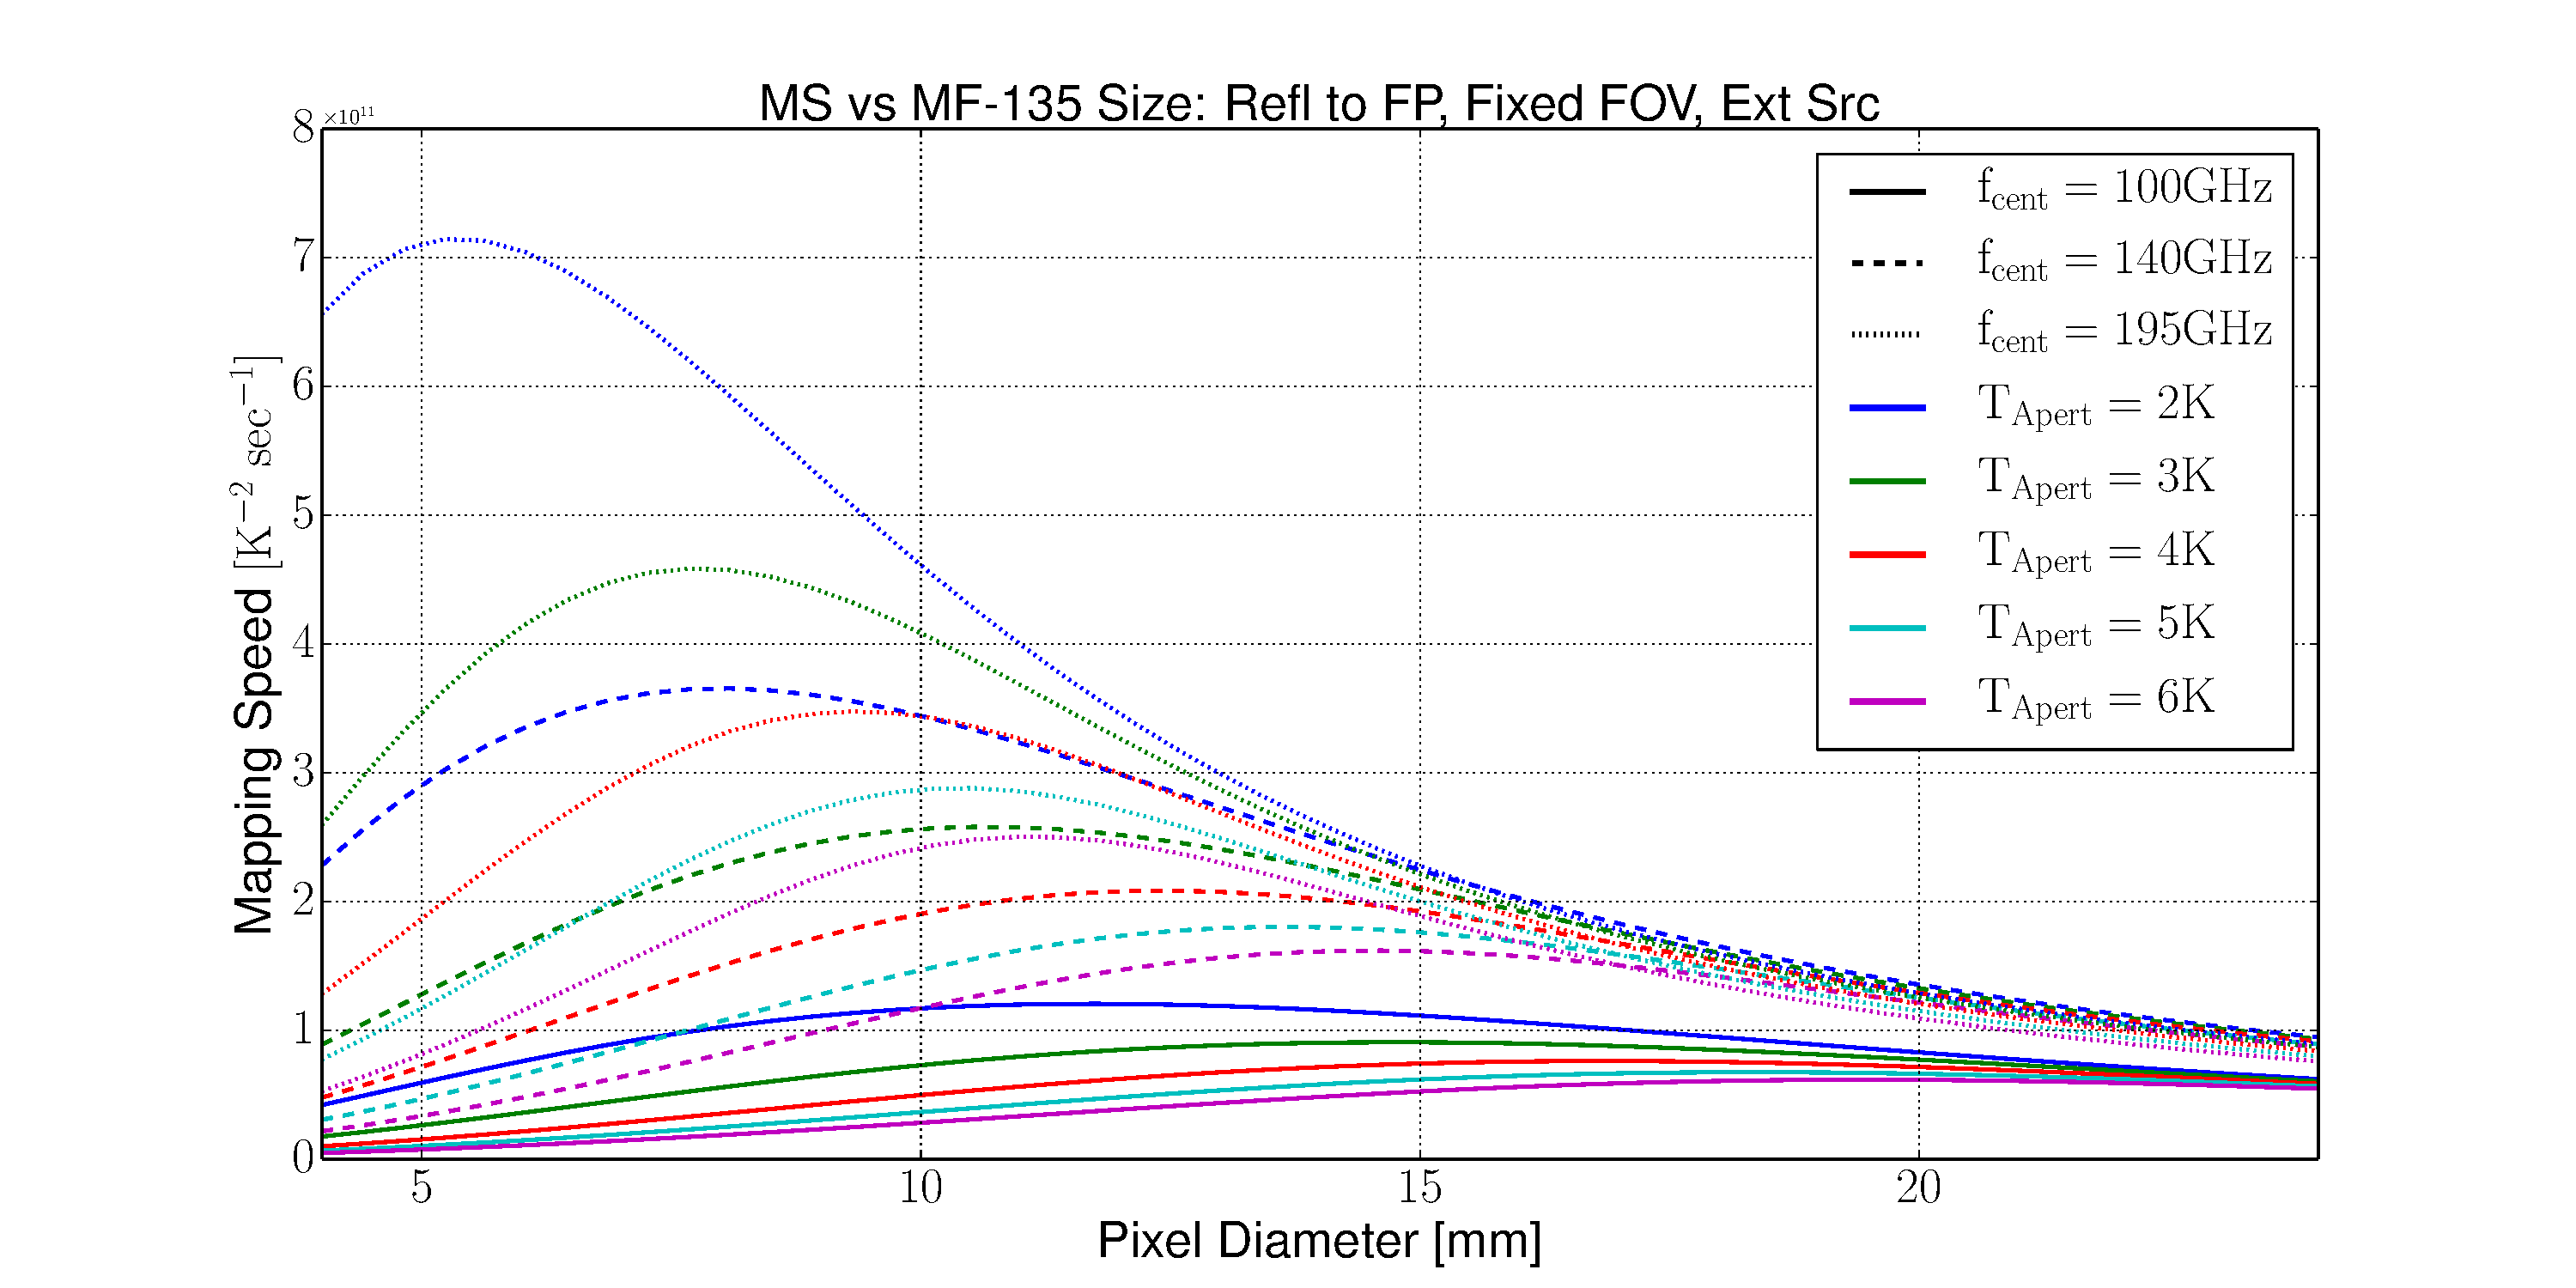
\includegraphics[width=1.1\textwidth, center]{PDF/LFT_MS_MF-135_coldRefl_fixFOV_extSrc.pdf}
	\caption{MF-135 mapping speed of an extended source as a function of pixel diameter for cold reflections and fixed FOV}
\end{figure}

\begin{figure}[H]
	\centering
	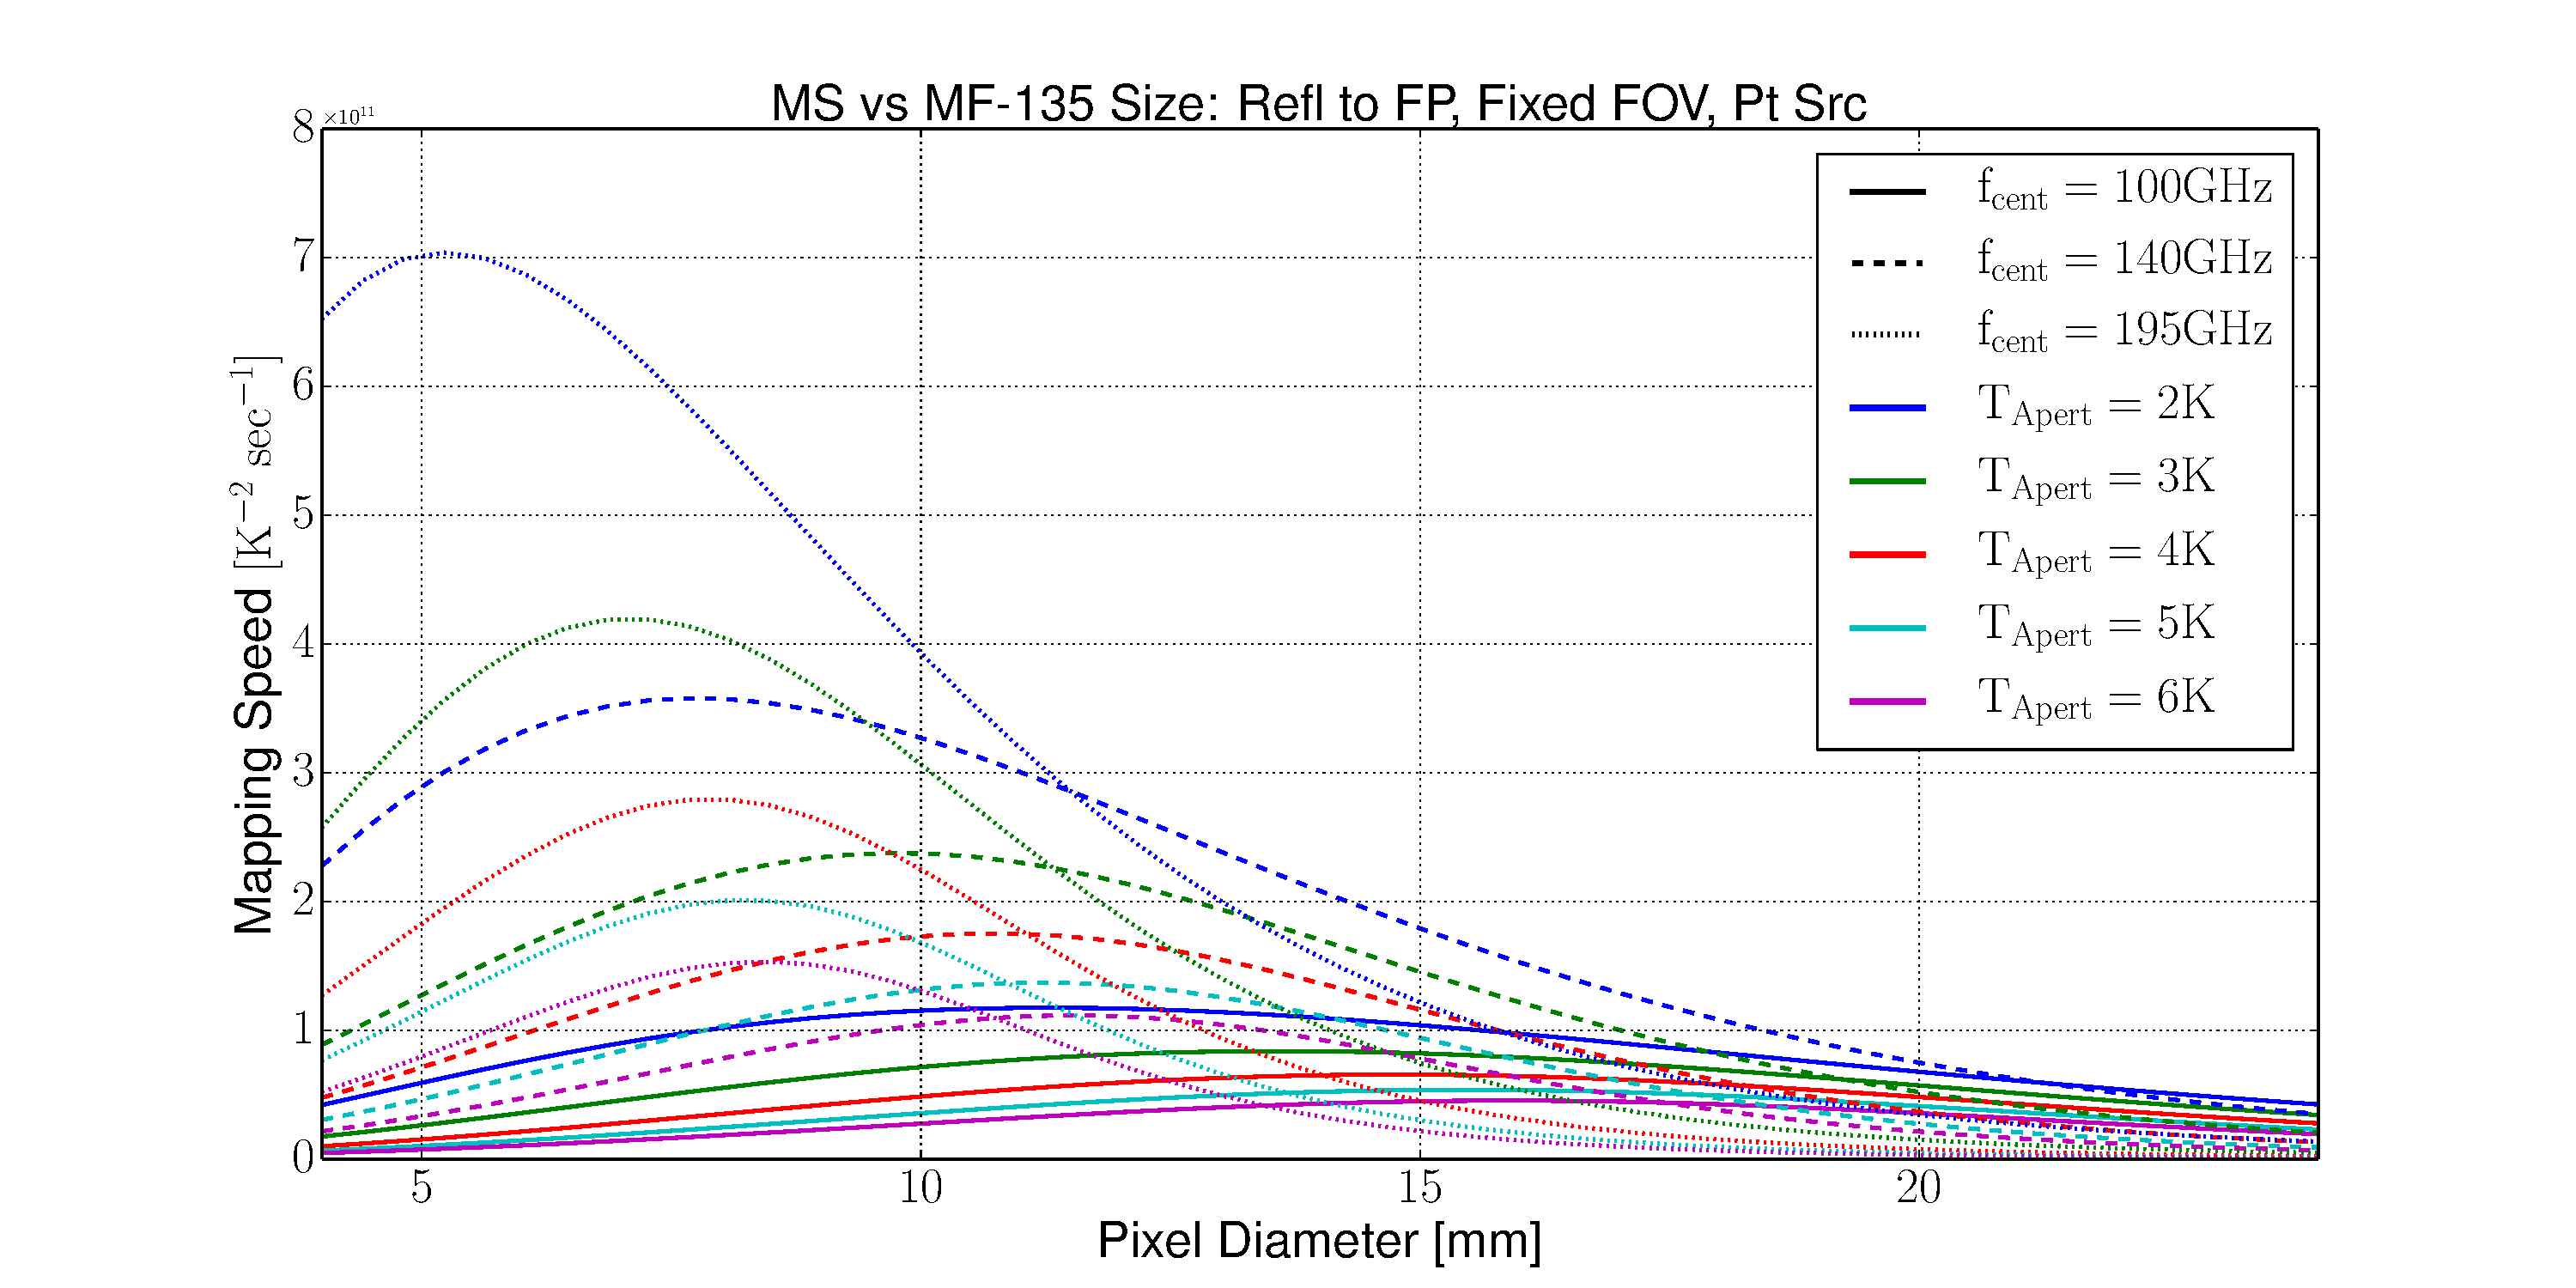
\includegraphics[width=1.1\textwidth, center]{PDF/LFT_MS_MF-135_coldRefl_fixFOV_ptSrc.pdf}
	\caption{MF-135 mapping speed of a point source as a function of pixel diameter for cold reflections and fixed FOV}
\end{figure}

%%%%%%%%%%%%%%%%%%% 

\subsubsection{MF-246}

\begin{figure}[H]
	\centering
	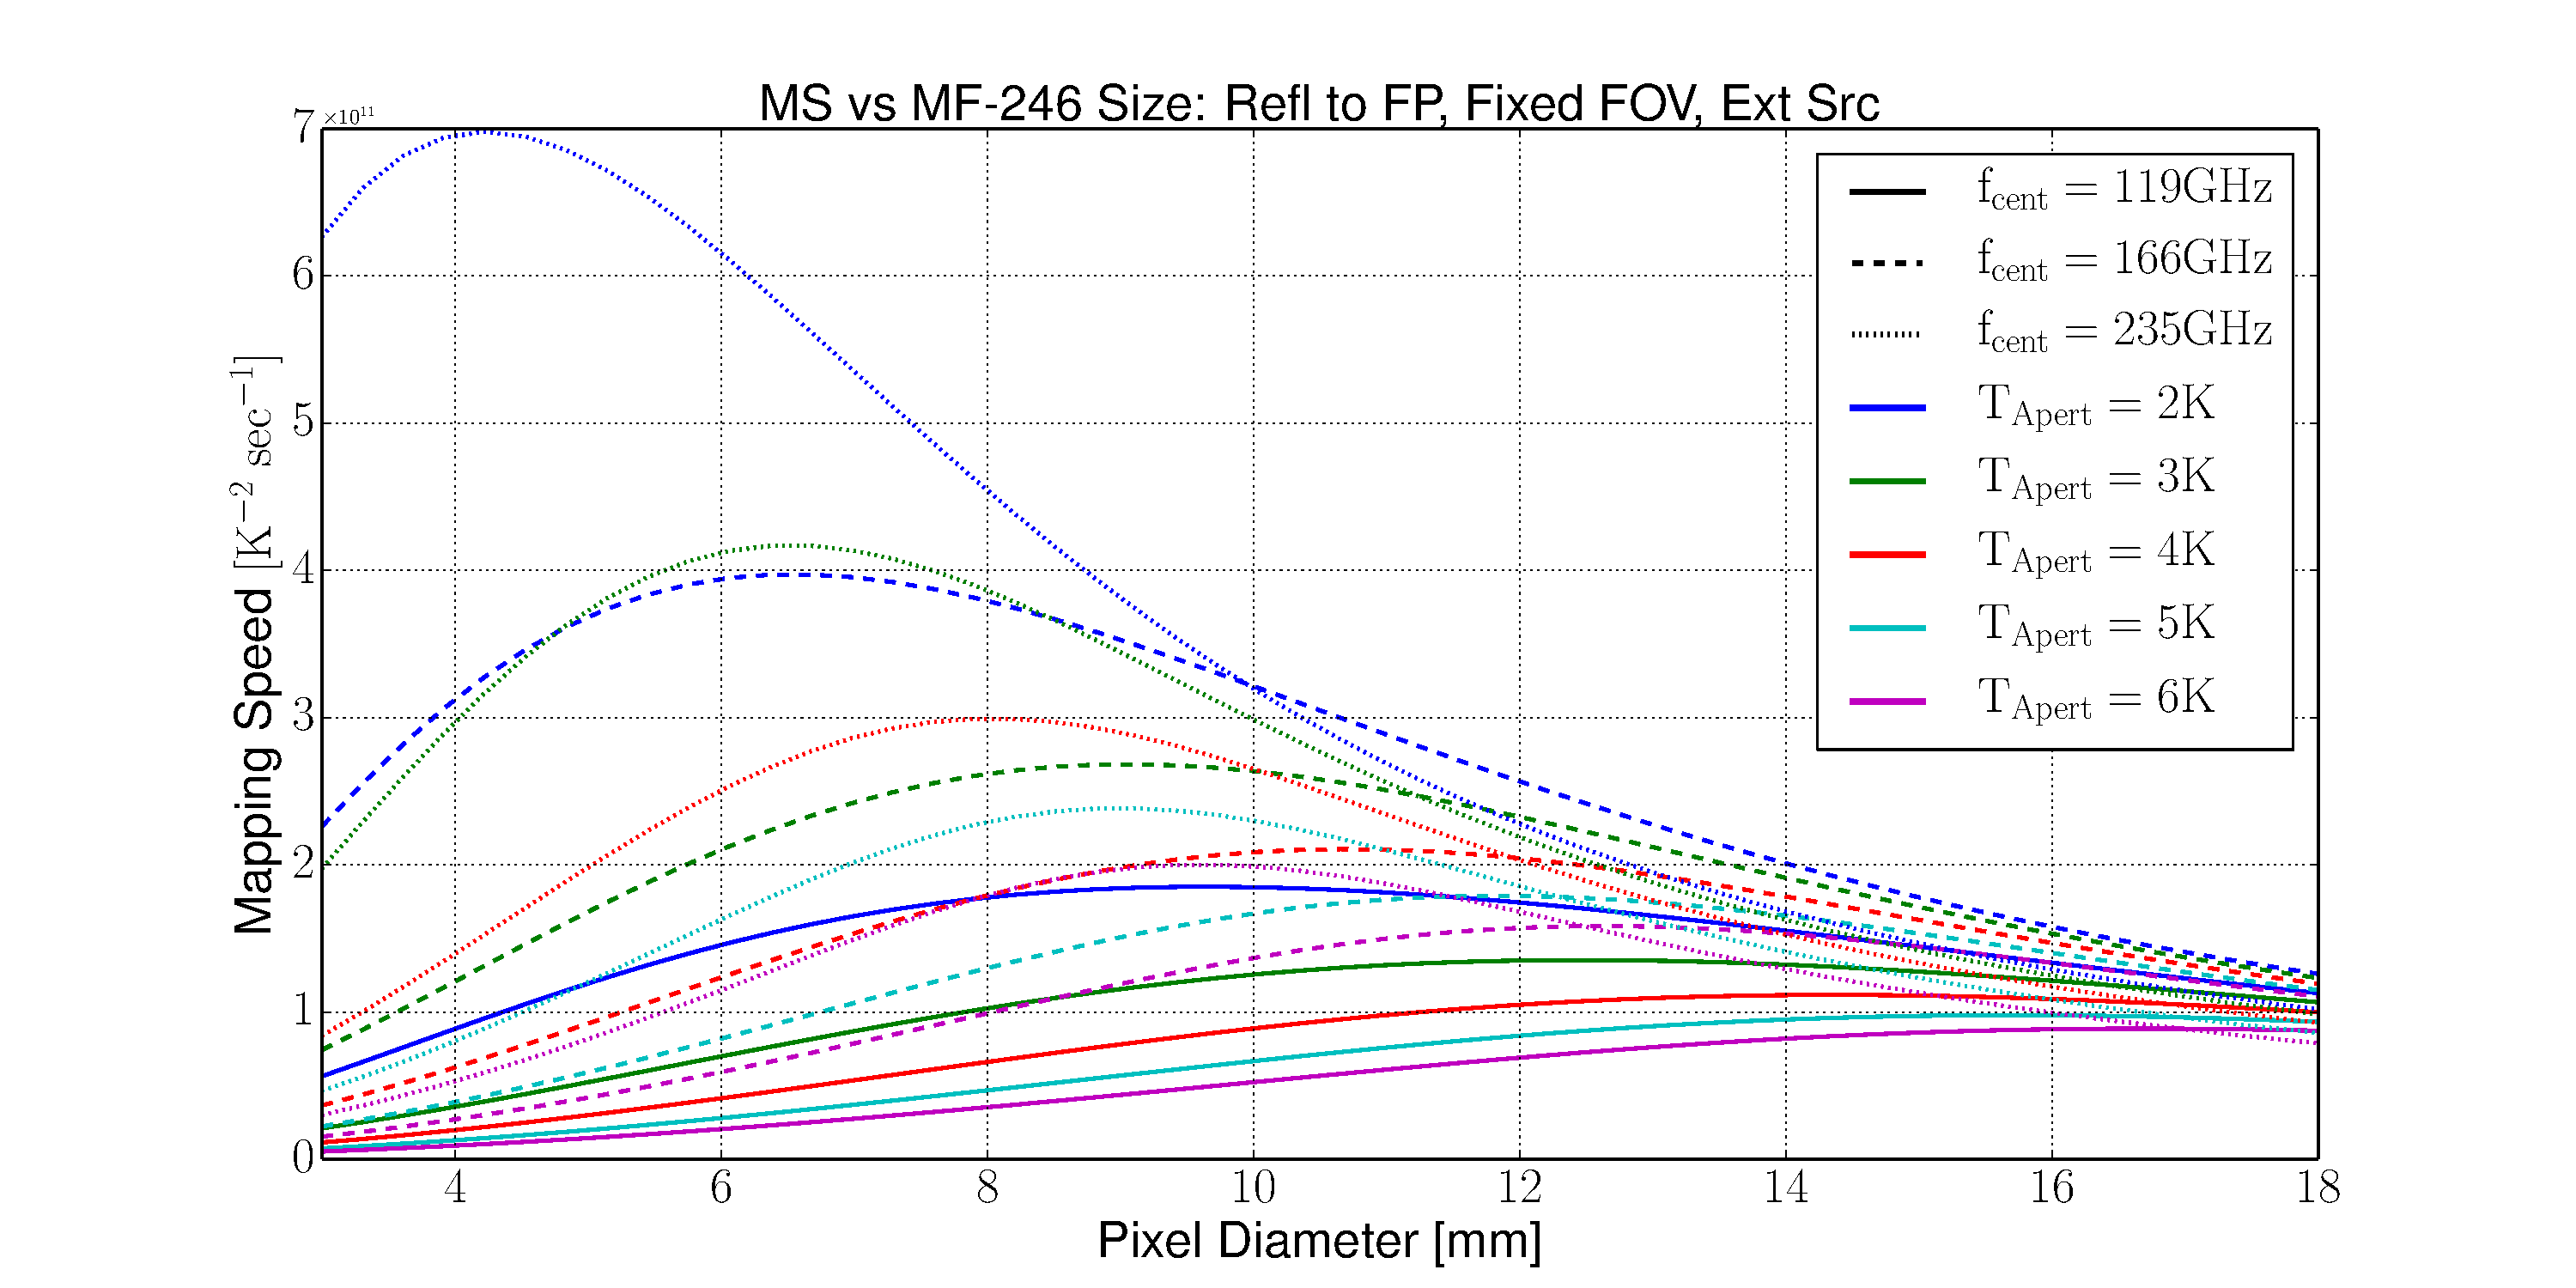
\includegraphics[width=1.1\textwidth, center]{PDF/LFT_MS_MF-246_coldRefl_fixFOV_extSrc.pdf}
	\caption{MF-246 mapping speed of an extended source as a function of pixel diameter for cold reflections and fixed FOV}
\end{figure}

\begin{figure}[H]
	\centering
	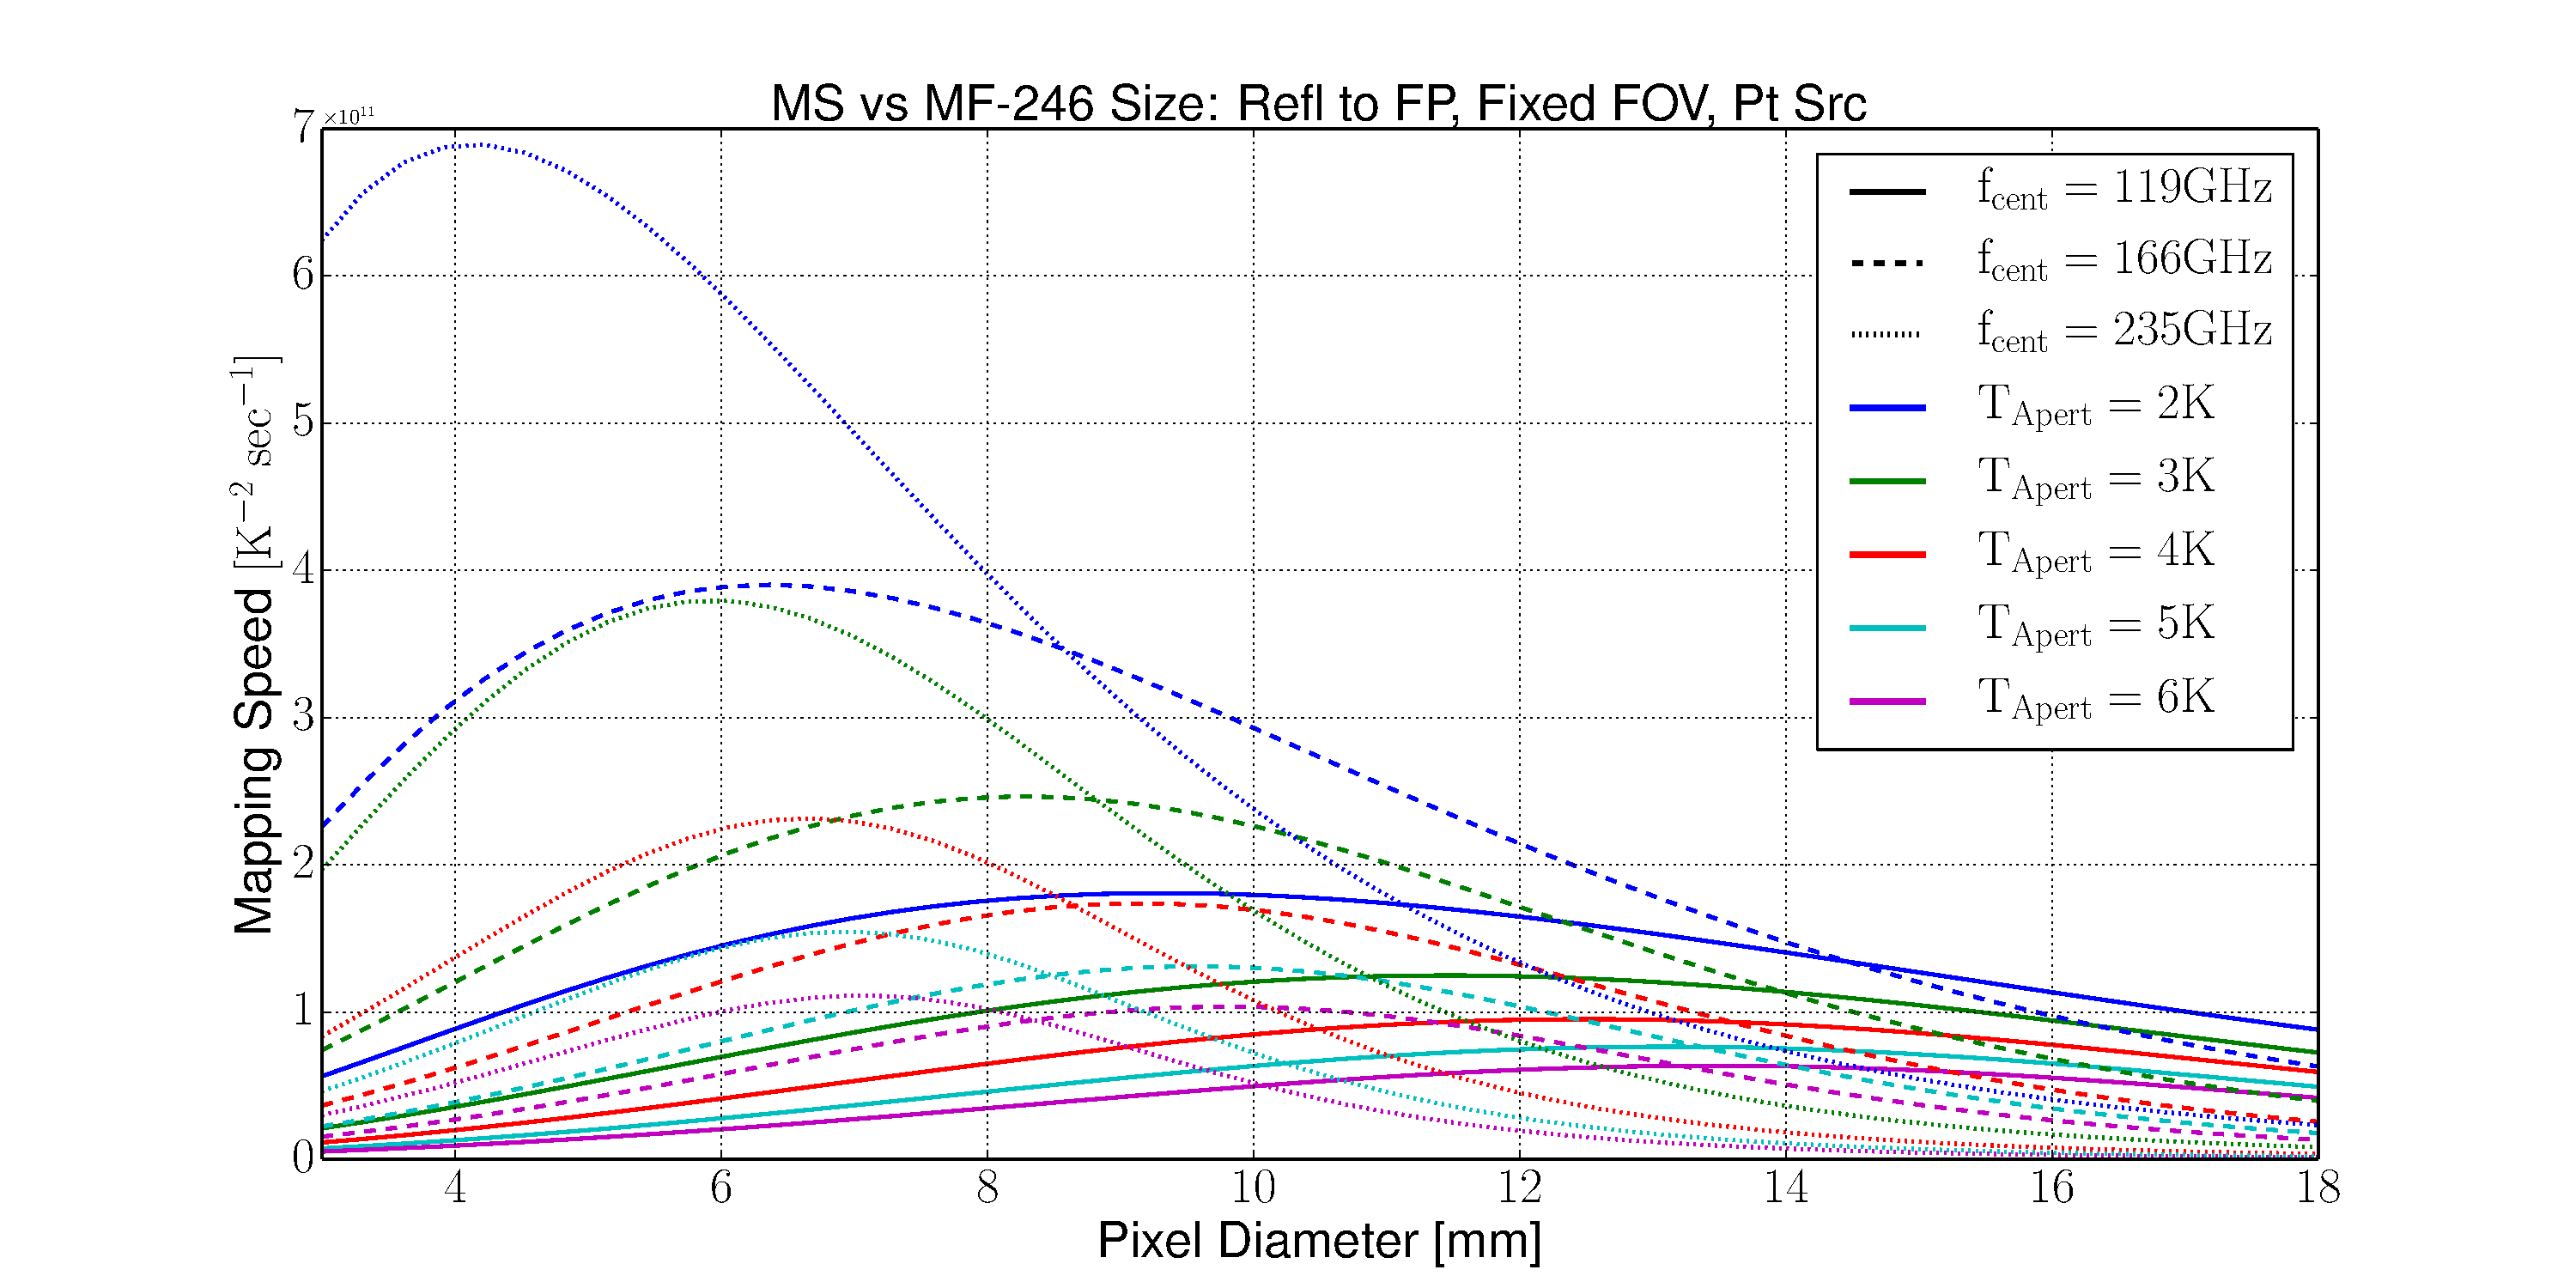
\includegraphics[width=1.1\textwidth, center]{PDF/LFT_MS_MF-246_coldRefl_fixFOV_ptSrc.pdf}
	\caption{MF-246 mapping speed of a point source as a function of pixel diameter for cold reflections and fixed FOV}
\end{figure}

%%%%%%%%%%%%%%%%%%%

\subsubsection{HFT}

\begin{figure}[H]
	\centering
	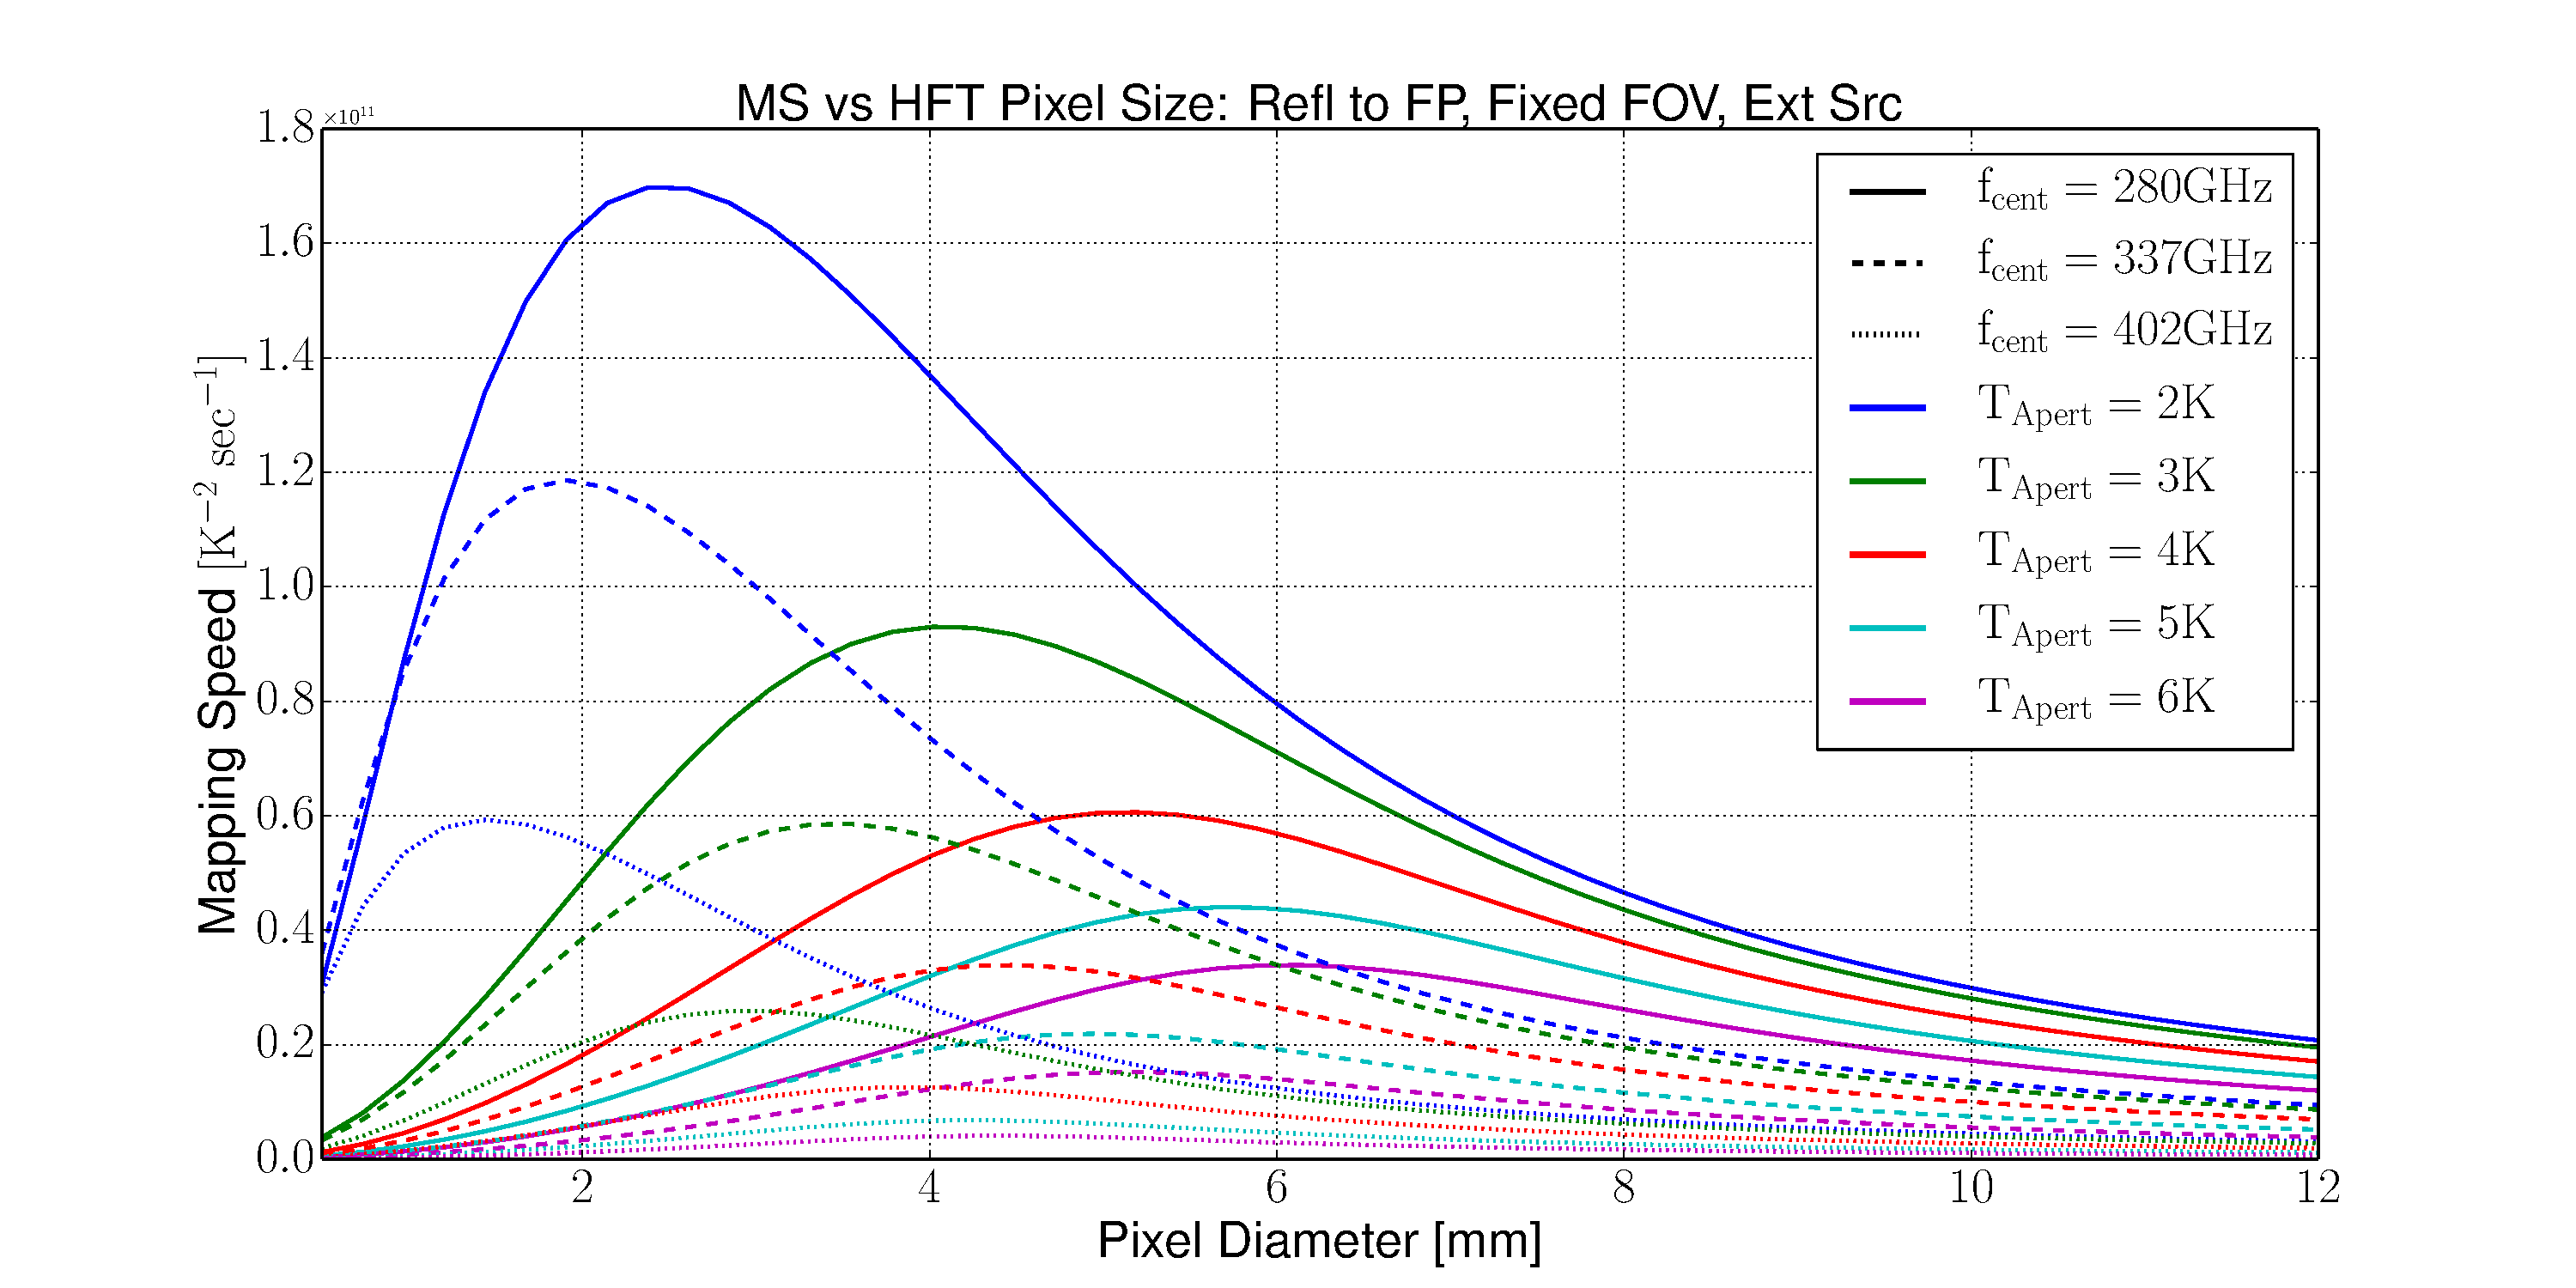
\includegraphics[width=1.1\textwidth, center]{PDF/HFT_MS_coldRefl_fixFOV_extSrc.pdf}
	\caption{HFT mapping speed of an extended source as a function of pixel diameter for cold reflections and fixed FOV}
\end{figure}

\begin{figure}[H]
	\centering
	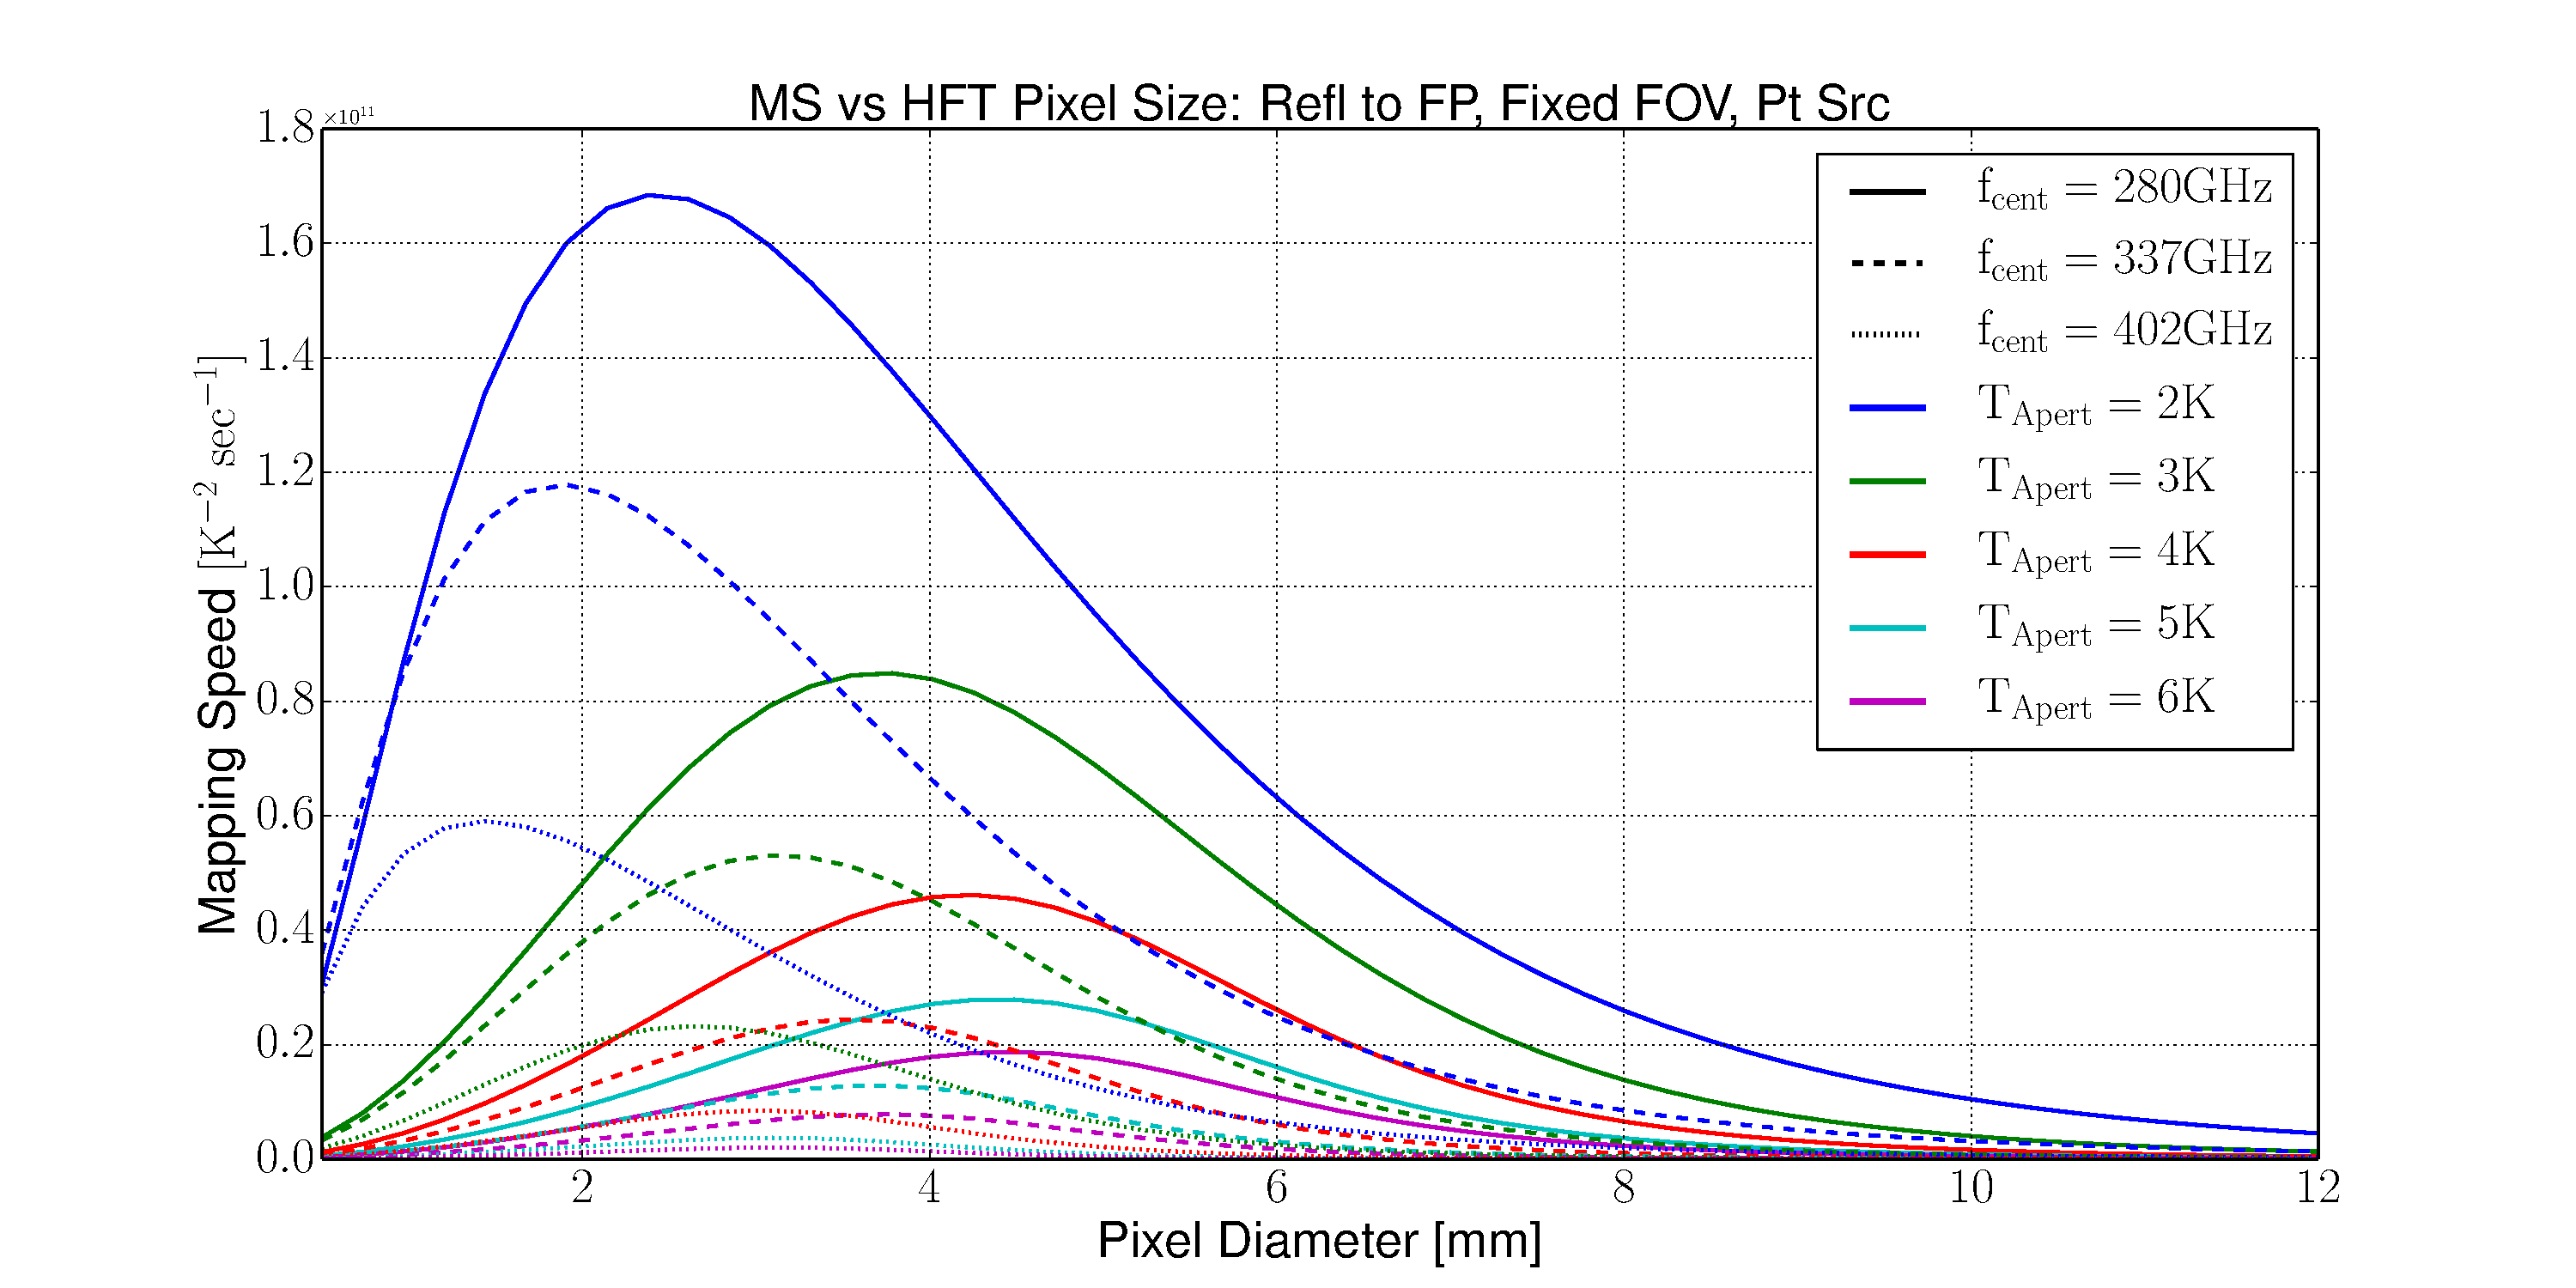
\includegraphics[width=1.1\textwidth, center]{PDF/HFT_MS_coldRefl_fixFOV_ptSrc.pdf}
	\caption{HFT mapping speed of a point source as a function of pixel diameter for cold reflections and fixed FOV}
\end{figure}


%%%%%%%%%%%%%%%%%%%%%%%%%%%%%%%%%%%%%

\subsection{Reflections Go to Focal Plane, Fixed Number of Detectors}

This subsection containts the results for the optimization of pixel diameters for the LFT and HFT given a fixed number of detectors and assuming all reflections go back to the focal plane.

\clearpage

%%%%%%%%%%%%%%%%%%%

\subsubsection{LF-135}

\begin{figure}[H]
	\centering
	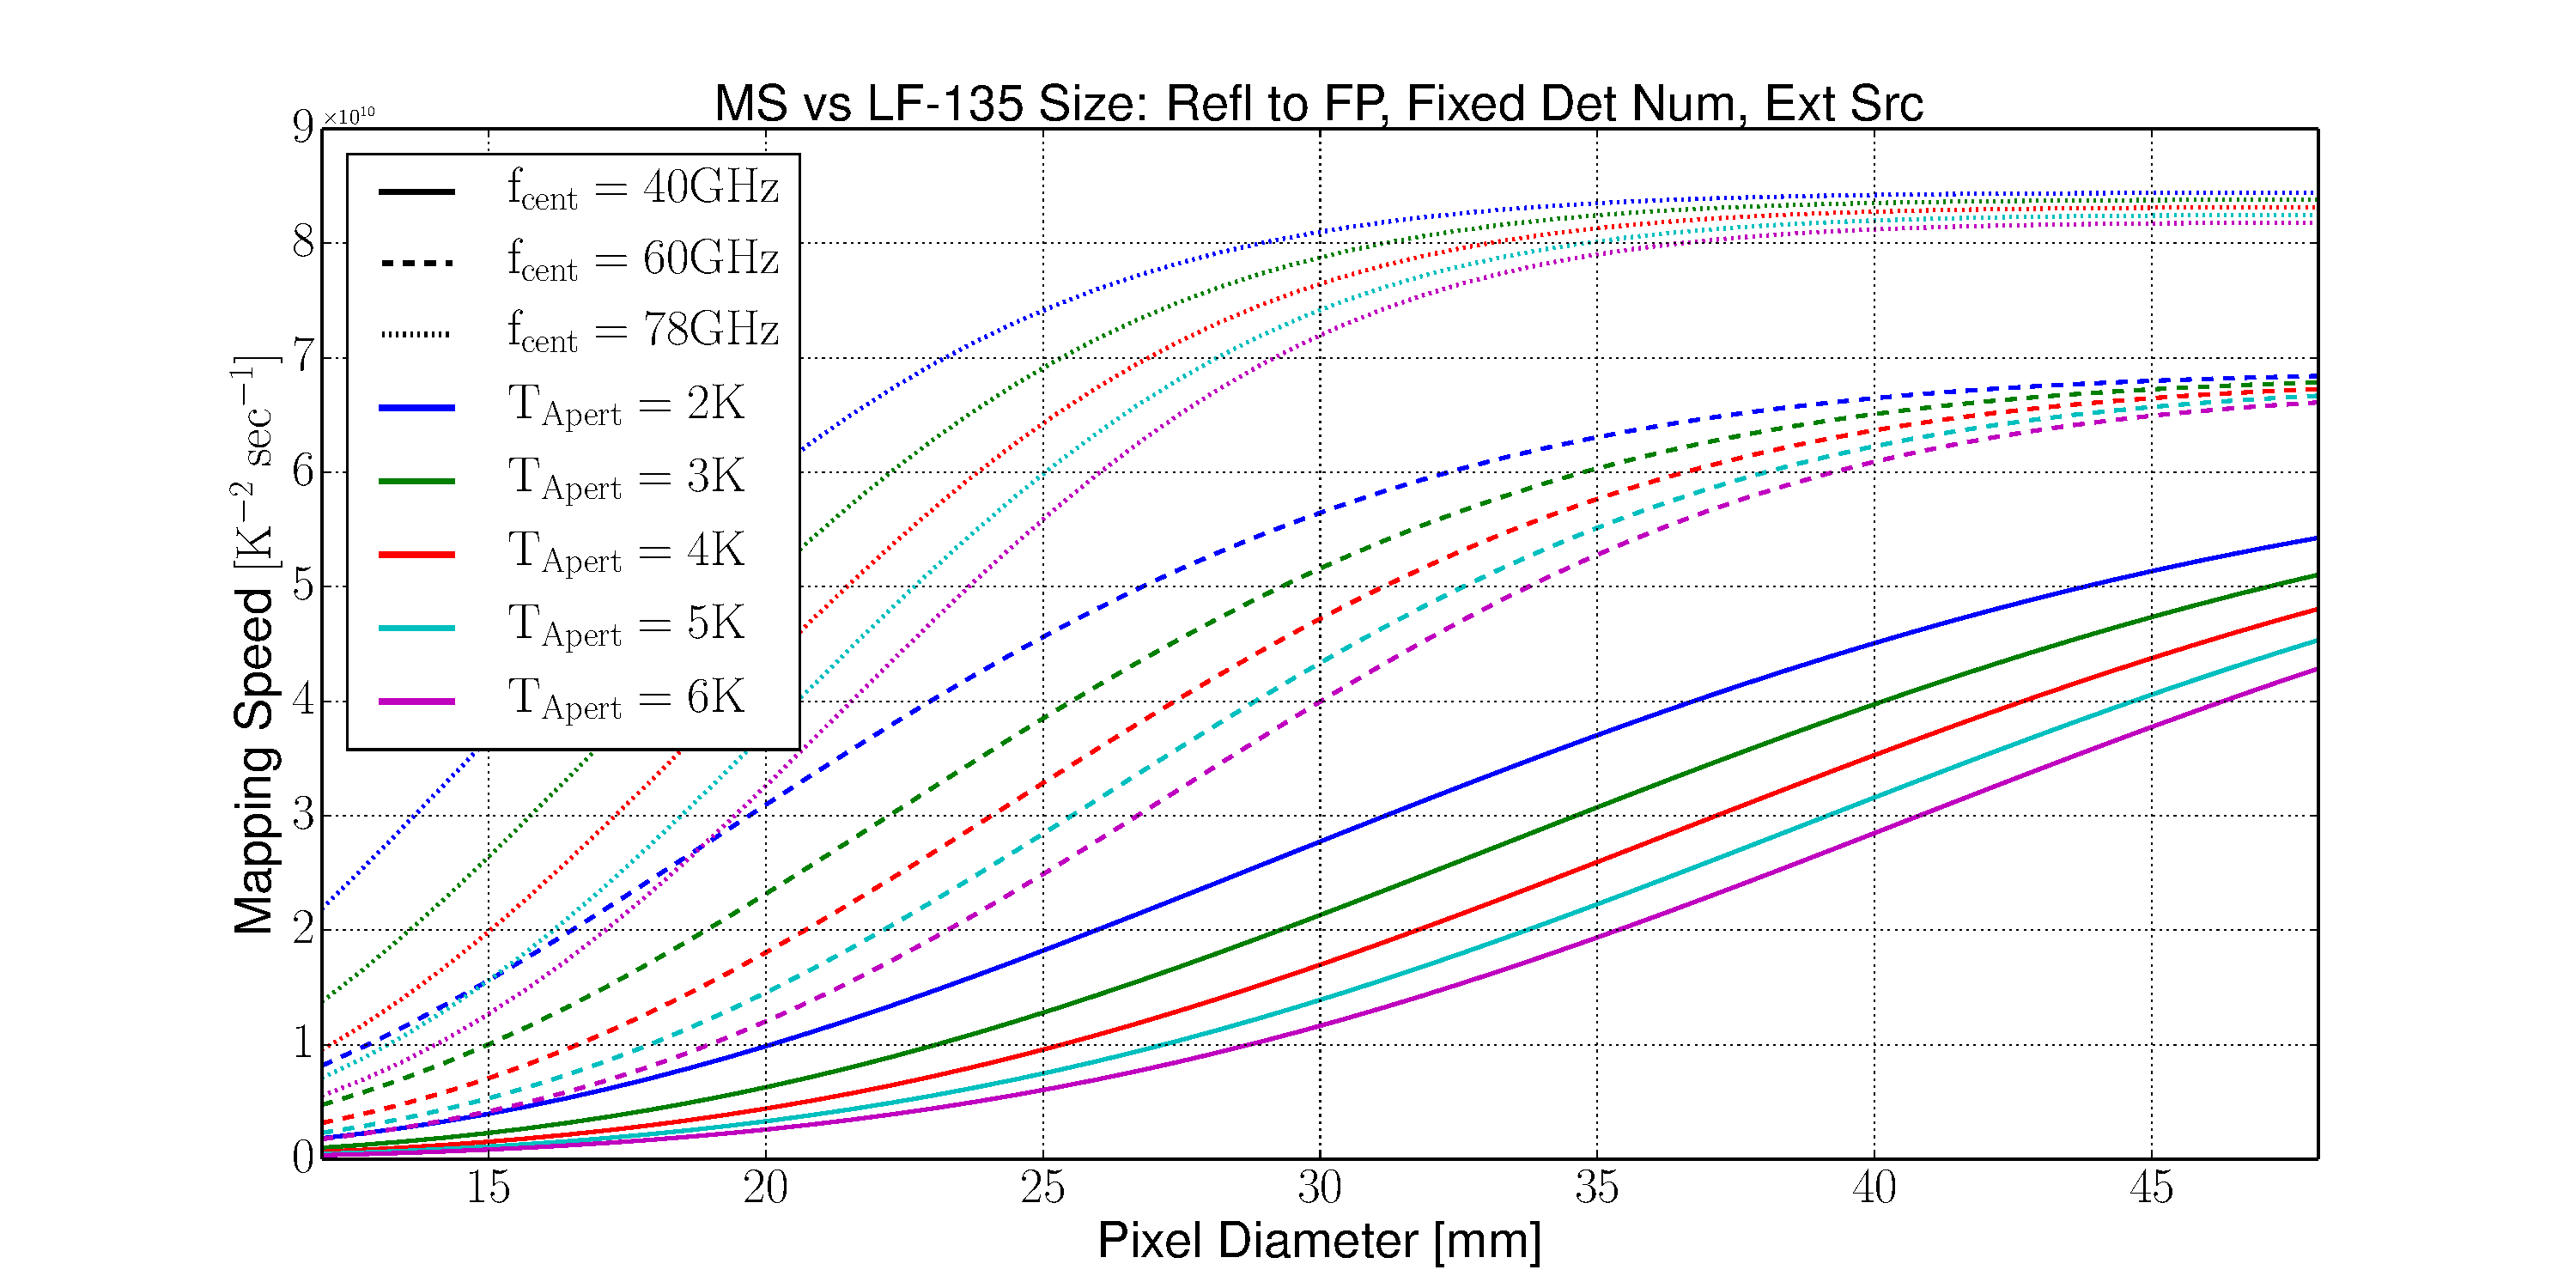
\includegraphics[width=1.1\textwidth, center]{PDF/LFT_MS_LF-135_coldRefl_fixDetNum_extSrc.pdf}
	\caption{LF-135 mapping speed of an extended source as a function of pixel diameter for cold reflections and fixed number of detectors}
\end{figure}

\begin{figure}[H]
	\centering
	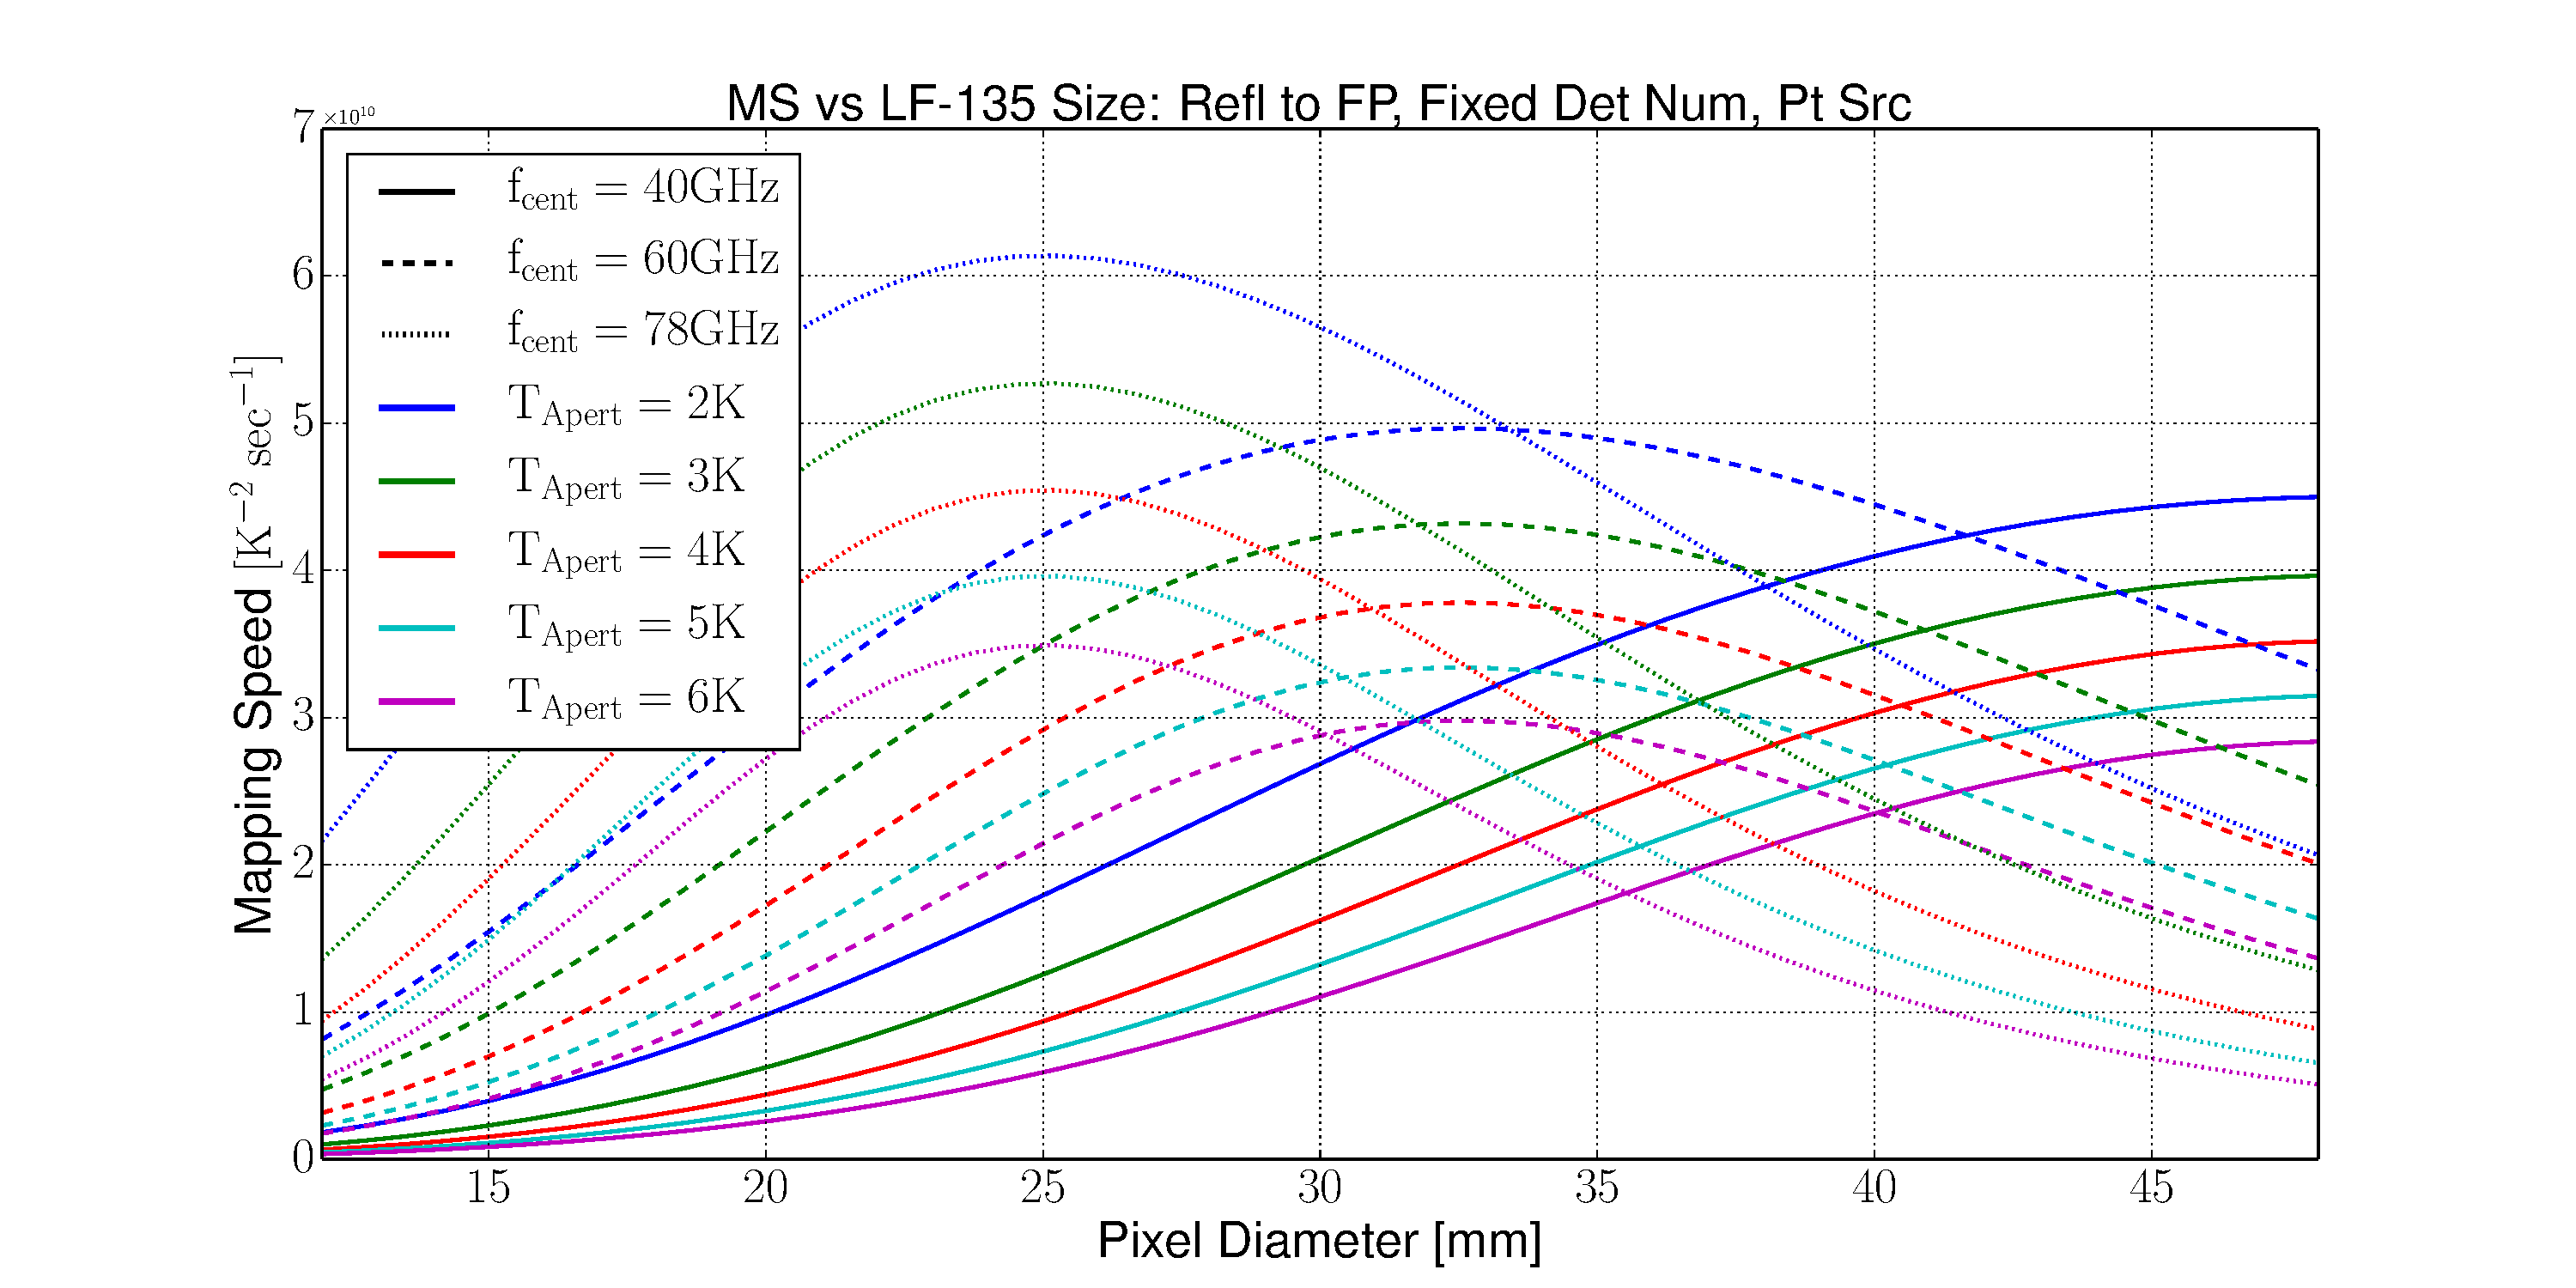
\includegraphics[width=1.1\textwidth, center]{PDF/LFT_MS_LF-135_coldRefl_fixDetNum_ptSrc.pdf}
	\caption{LF-135 mapping speed of a point source as a function of pixel diameter for cold reflections and fixed number of detectors}
\end{figure}

%%%%%%%%%%%%%%%%%%%

\subsubsection{LF-246}

\begin{figure}[H]
	\centering
	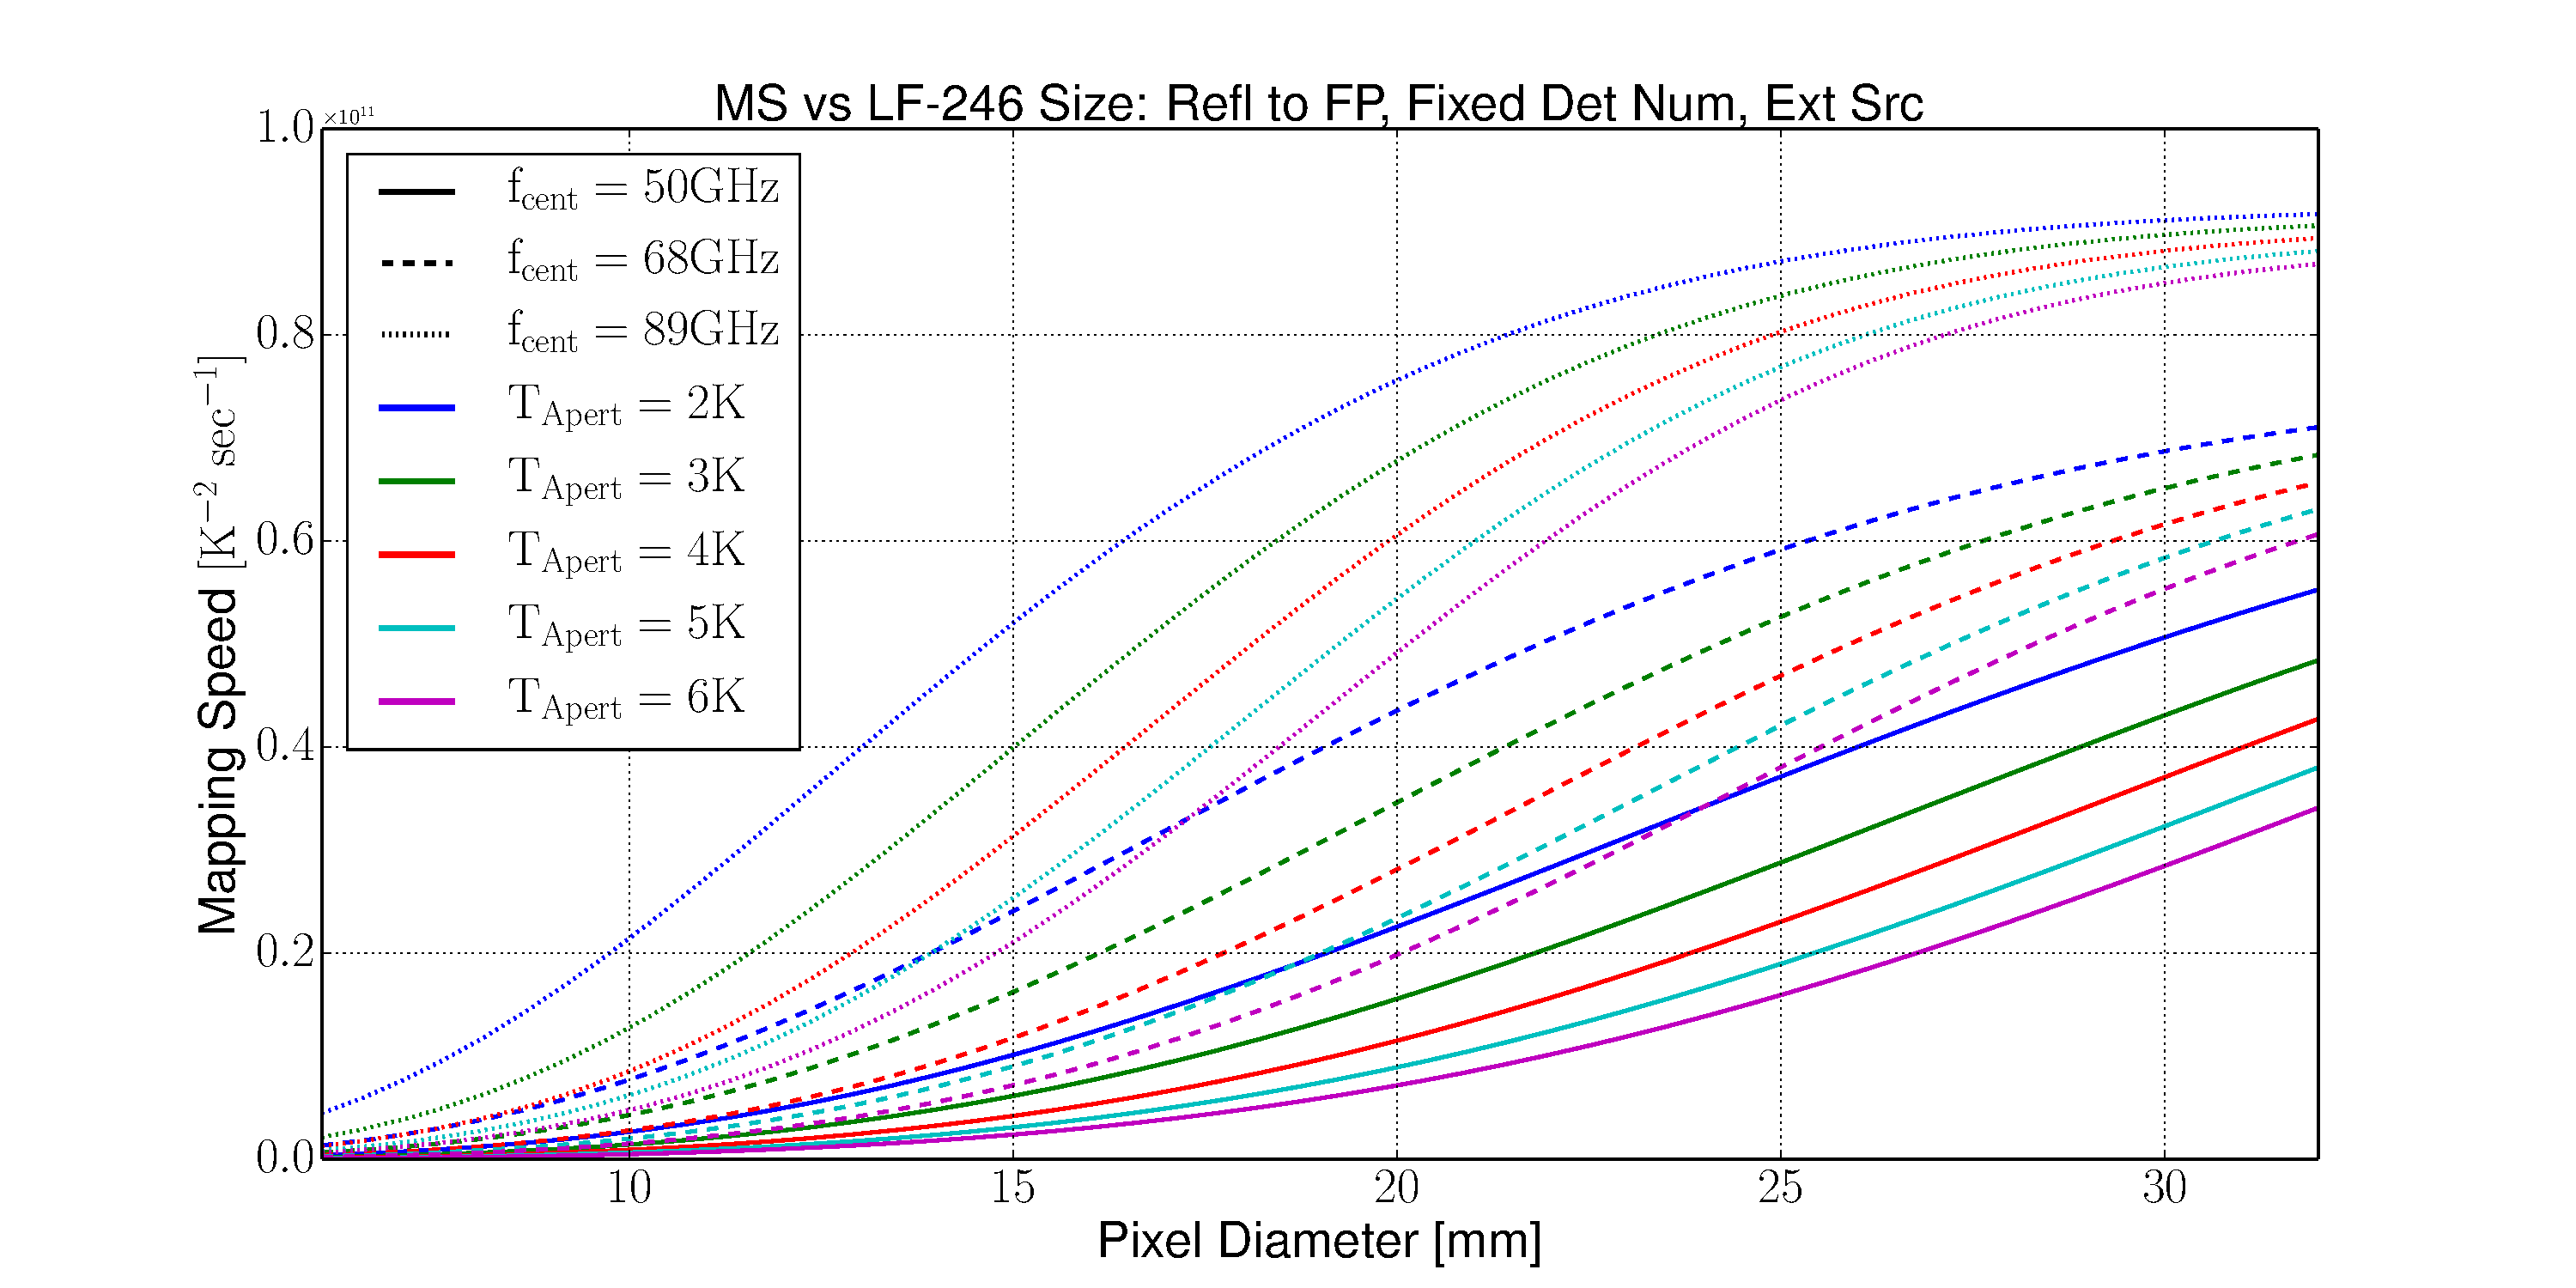
\includegraphics[width=1.1\textwidth, center]{PDF/LFT_MS_LF-246_coldRefl_fixDetNum_extSrc.pdf}
	\caption{LF-246 mapping speed of an extended source as a function of pixel diameter for cold reflections and fixed number of detectors}
\end{figure}

\begin{figure}[H]
	\centering
	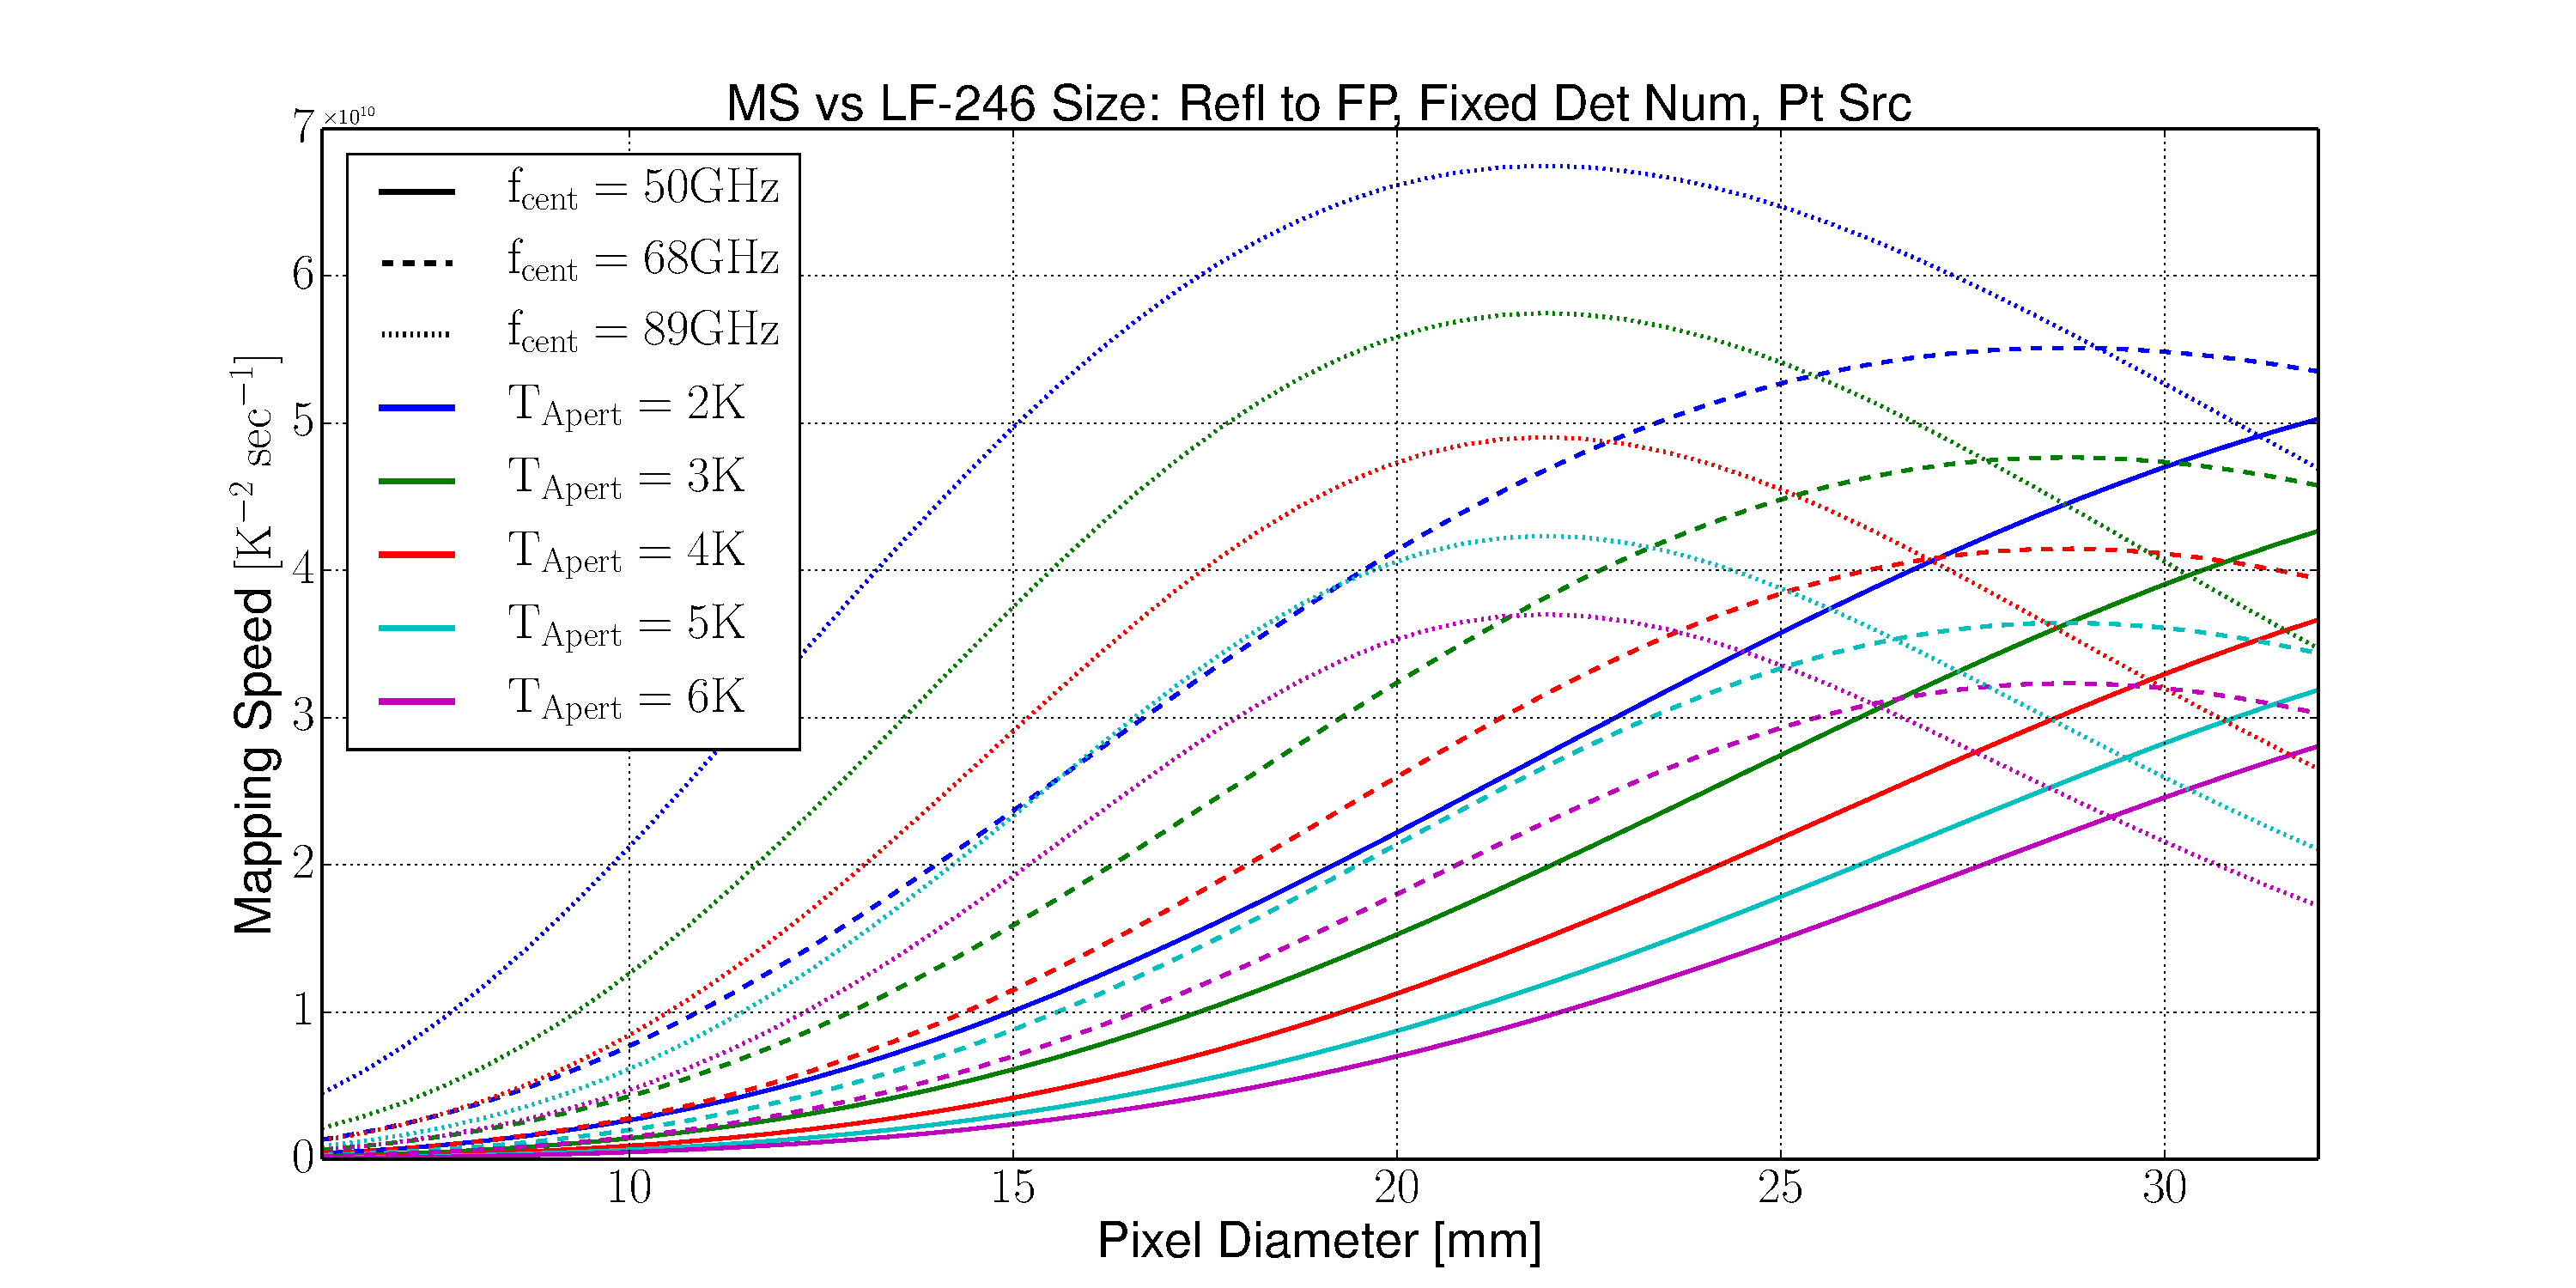
\includegraphics[width=1.1\textwidth, center]{PDF/LFT_MS_LF-246_coldRefl_fixDetNum_ptSrc.pdf}
	\caption{LF-246 mapping speed of a point source as a function of pixel diameter for cold reflections and fixed number of detectors}
\end{figure}

%%%%%%%%%%%%%%%%%%%

\subsubsection{MF-135}

\begin{figure}[H]
	\centering
	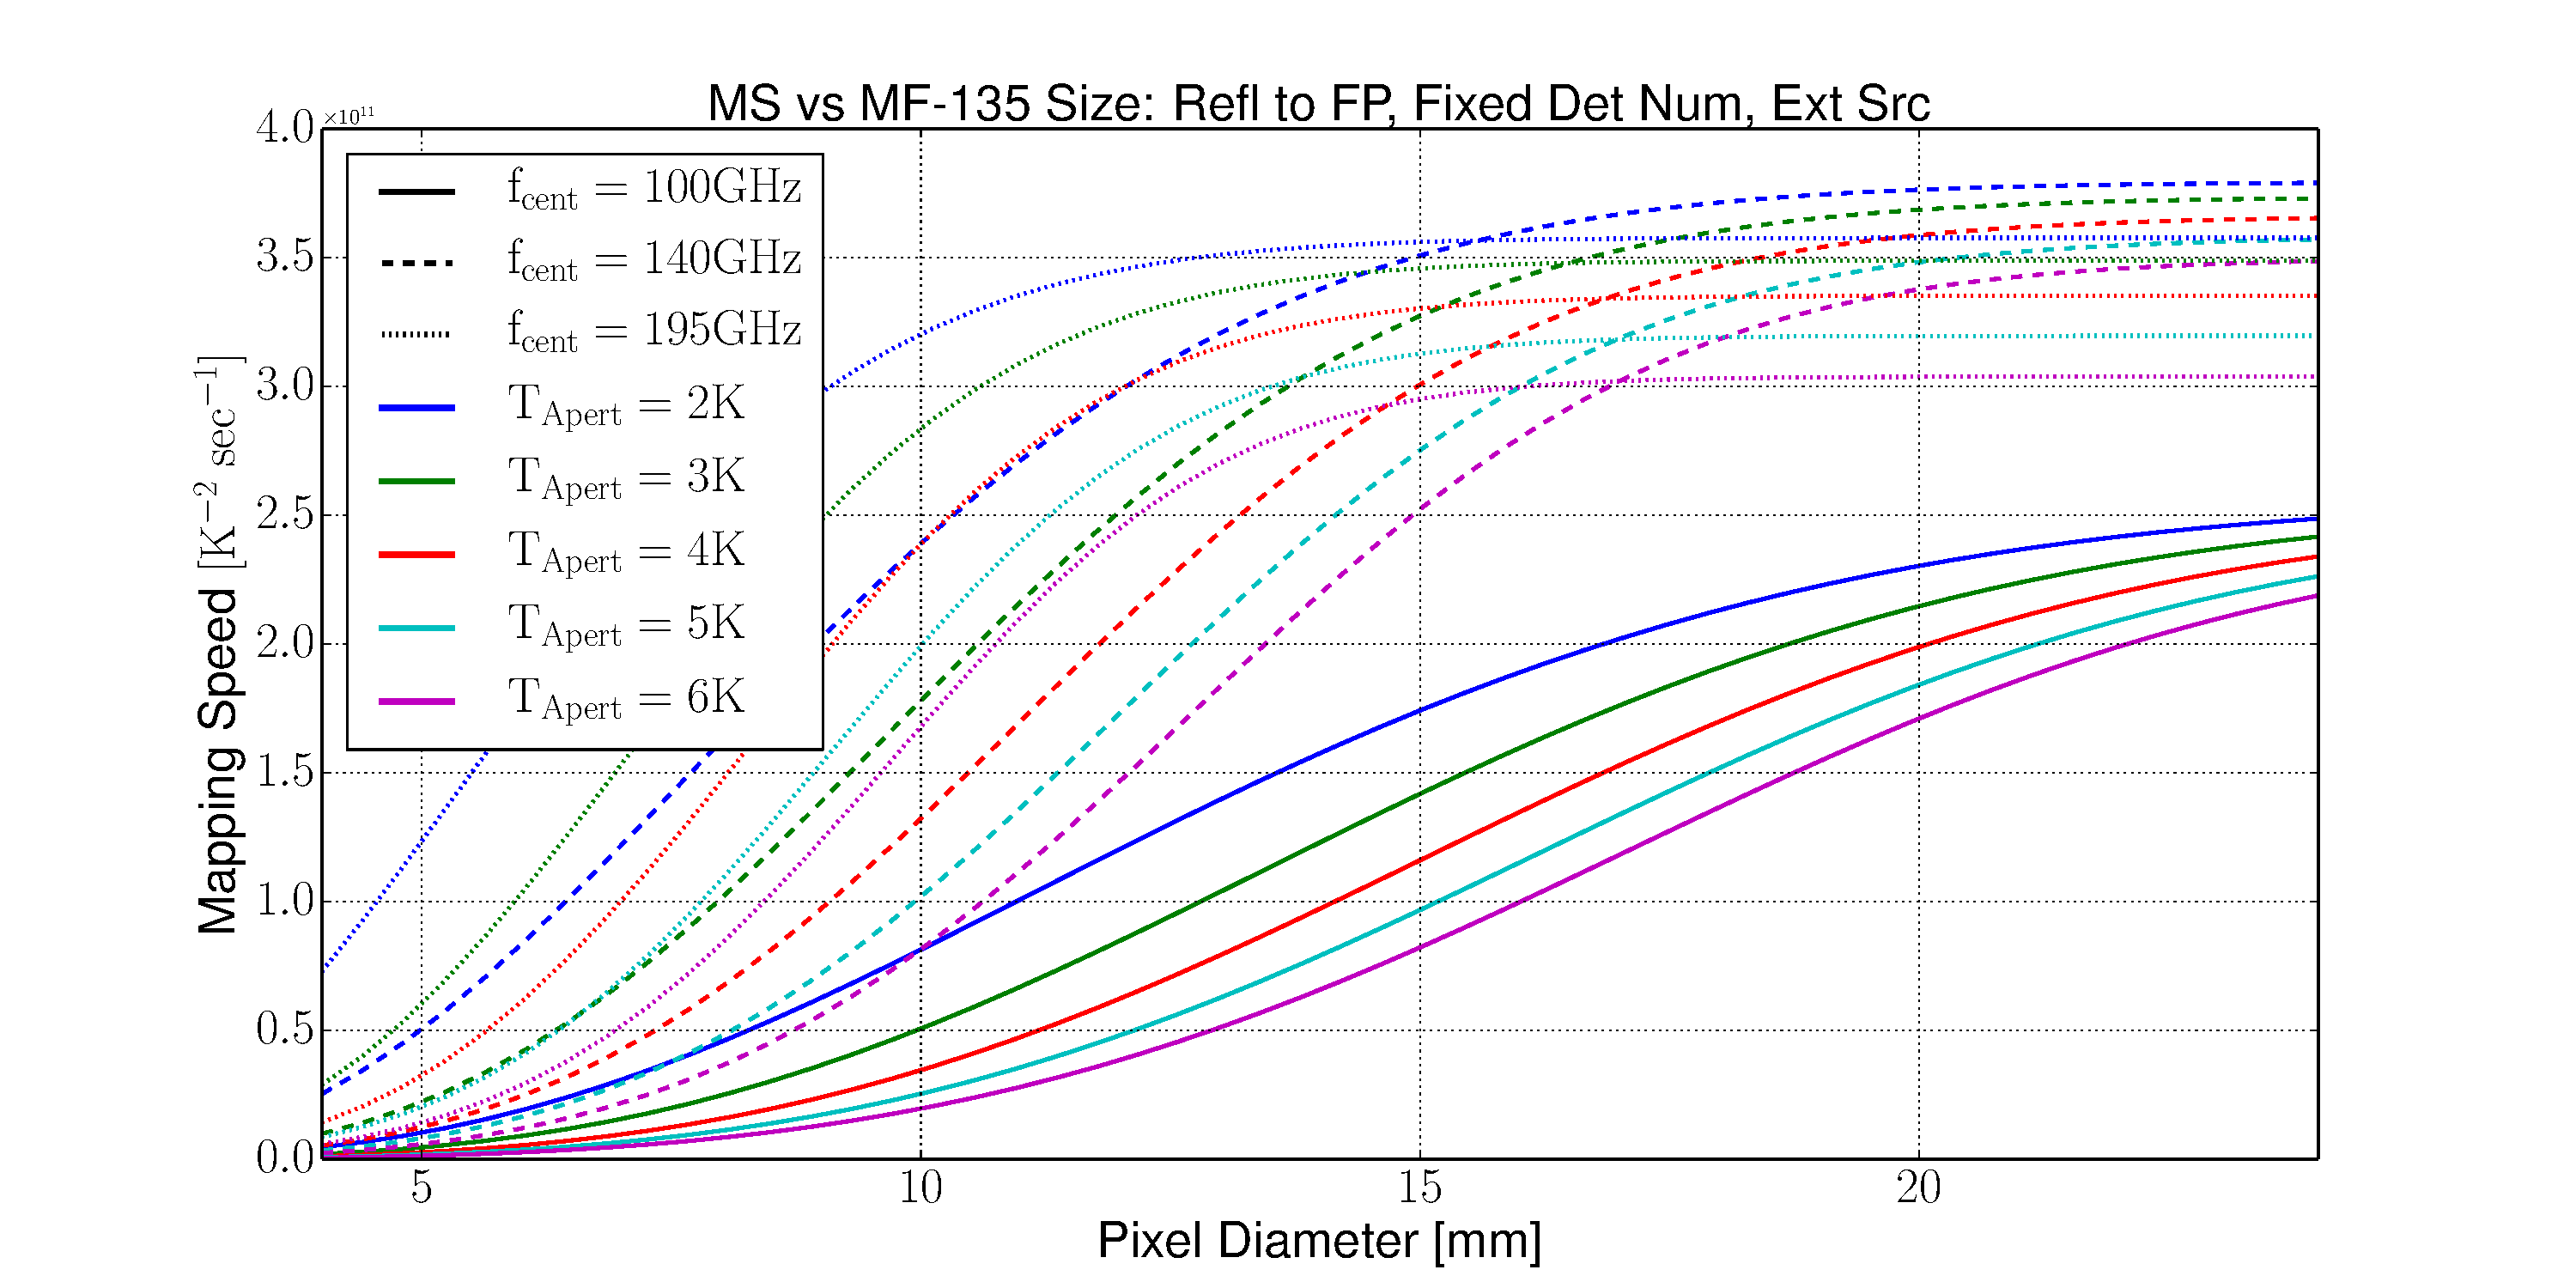
\includegraphics[width=1.1\textwidth, center]{PDF/LFT_MS_MF-135_coldRefl_fixDetNum_extSrc.pdf}
	\caption{MF-135 mapping speed of an extended source as a function of pixel diameter for cold reflections and fixed number of detectors}
\end{figure}

\begin{figure}[H]
	\centering
	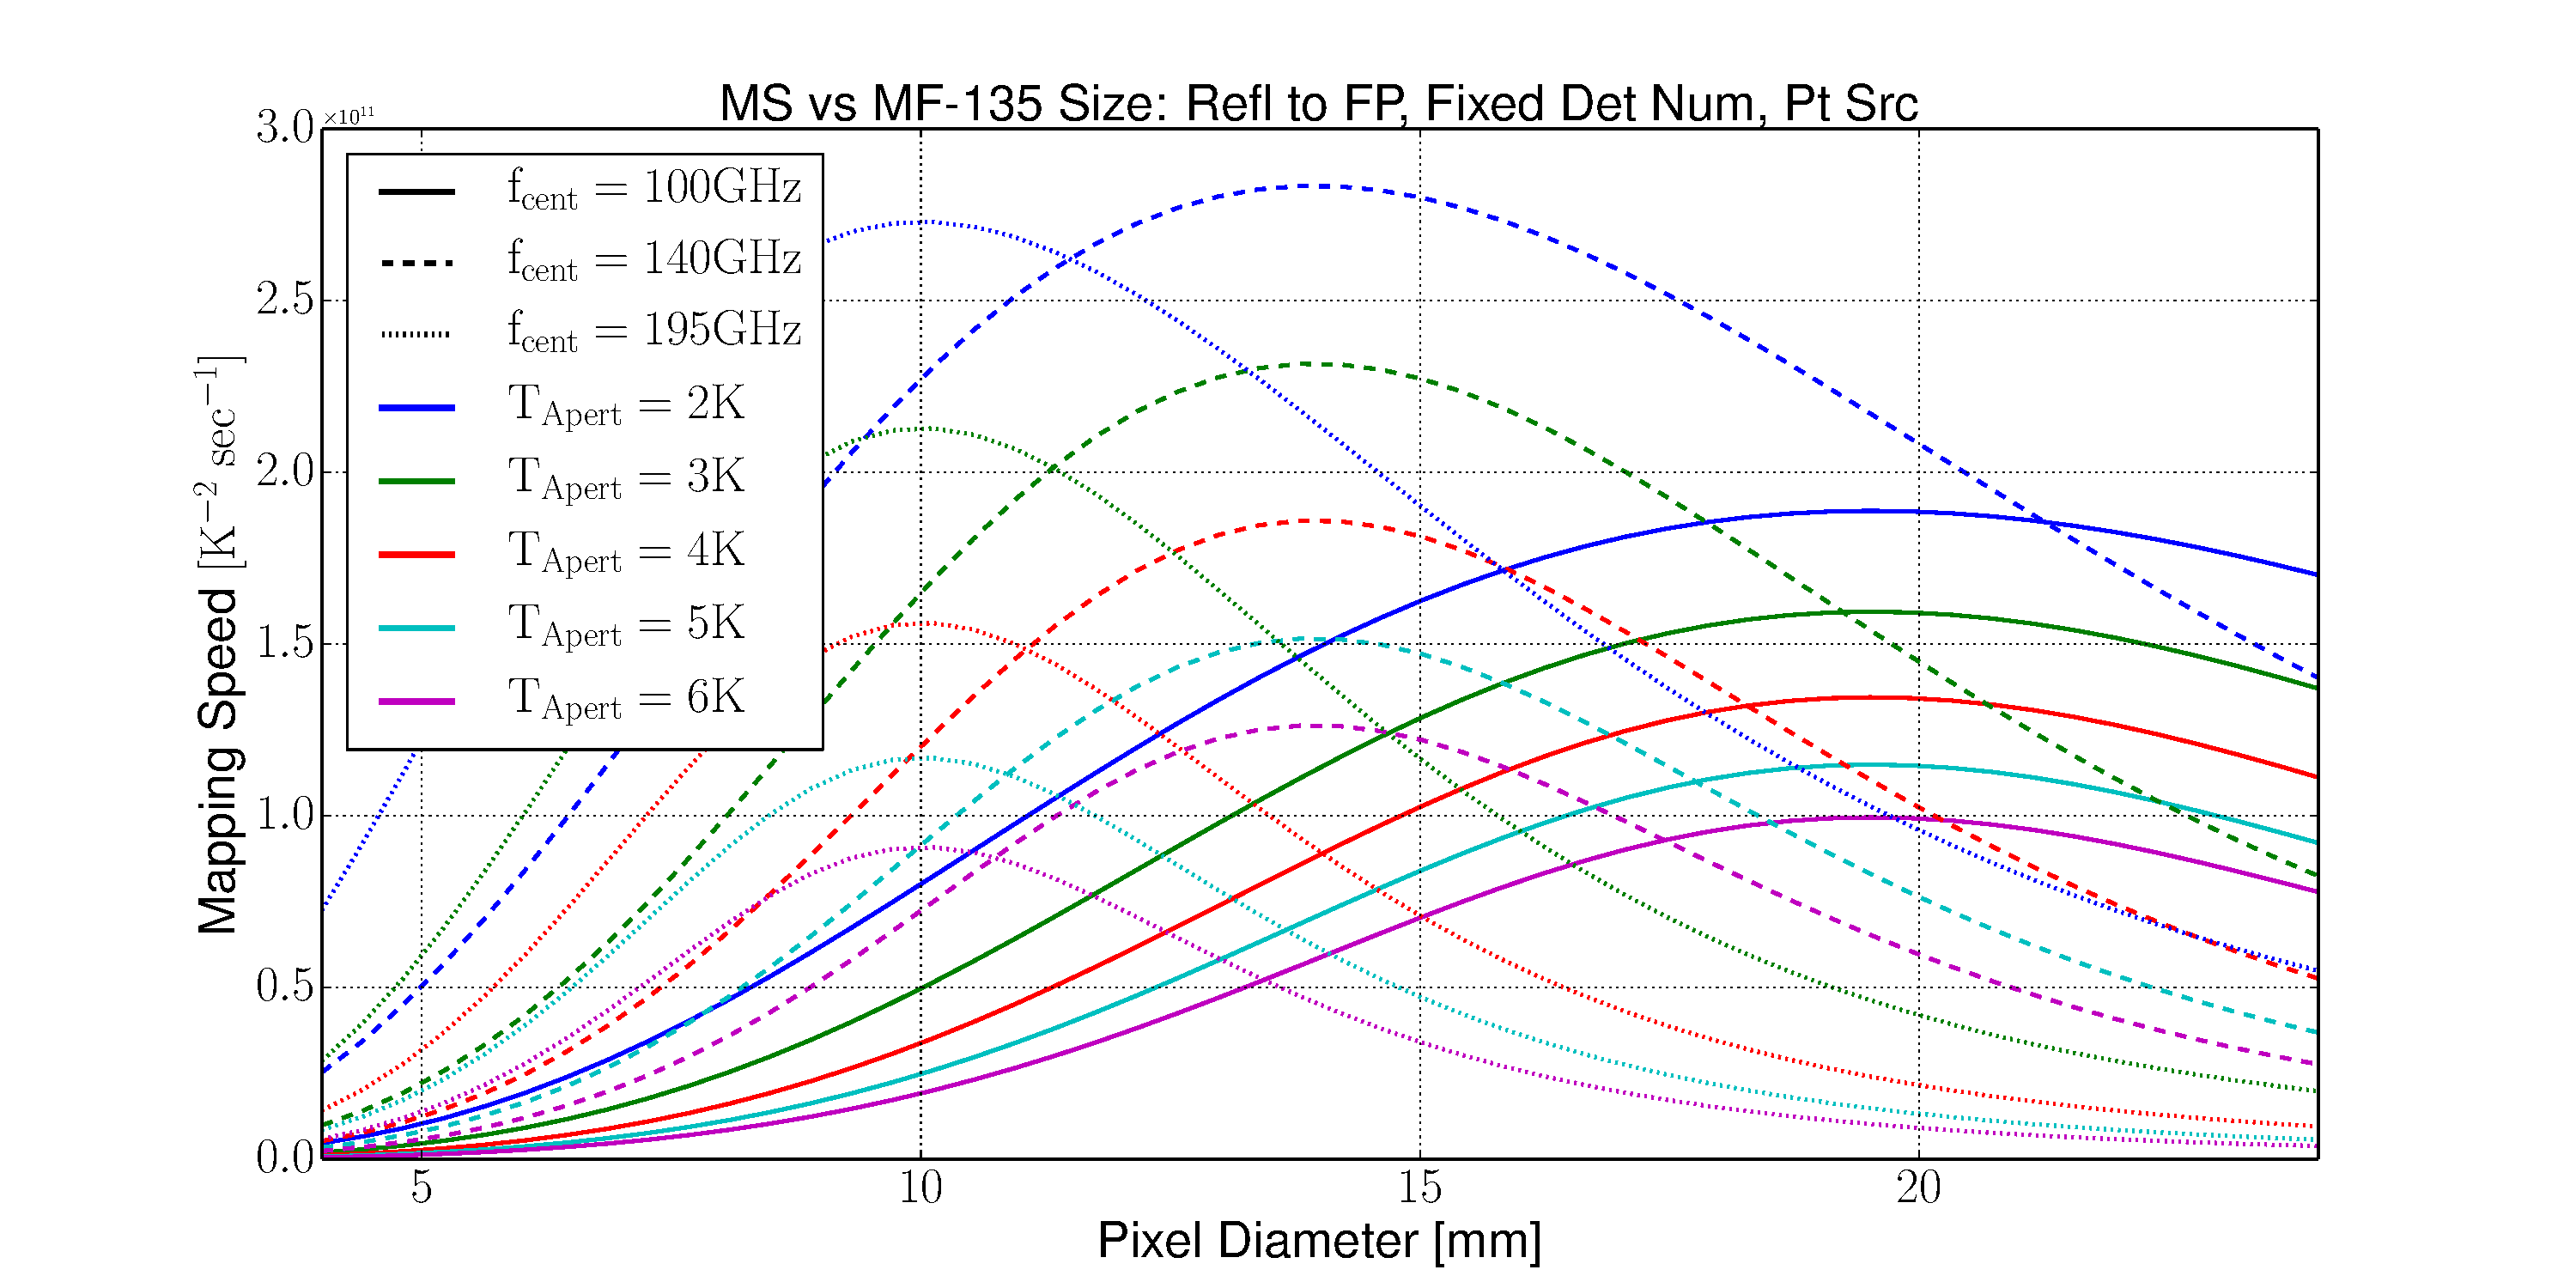
\includegraphics[width=1.1\textwidth, center]{PDF/LFT_MS_MF-135_coldRefl_fixDetNum_ptSrc.pdf}
	\caption{MF-135 mapping speed of a point source as a function of pixel diameter for cold reflections and fixed number of detectors}
\end{figure}

%%%%%%%%%%%%%%%%%%%

\subsubsection{MF-246}

\begin{figure}[H]
	\centering
	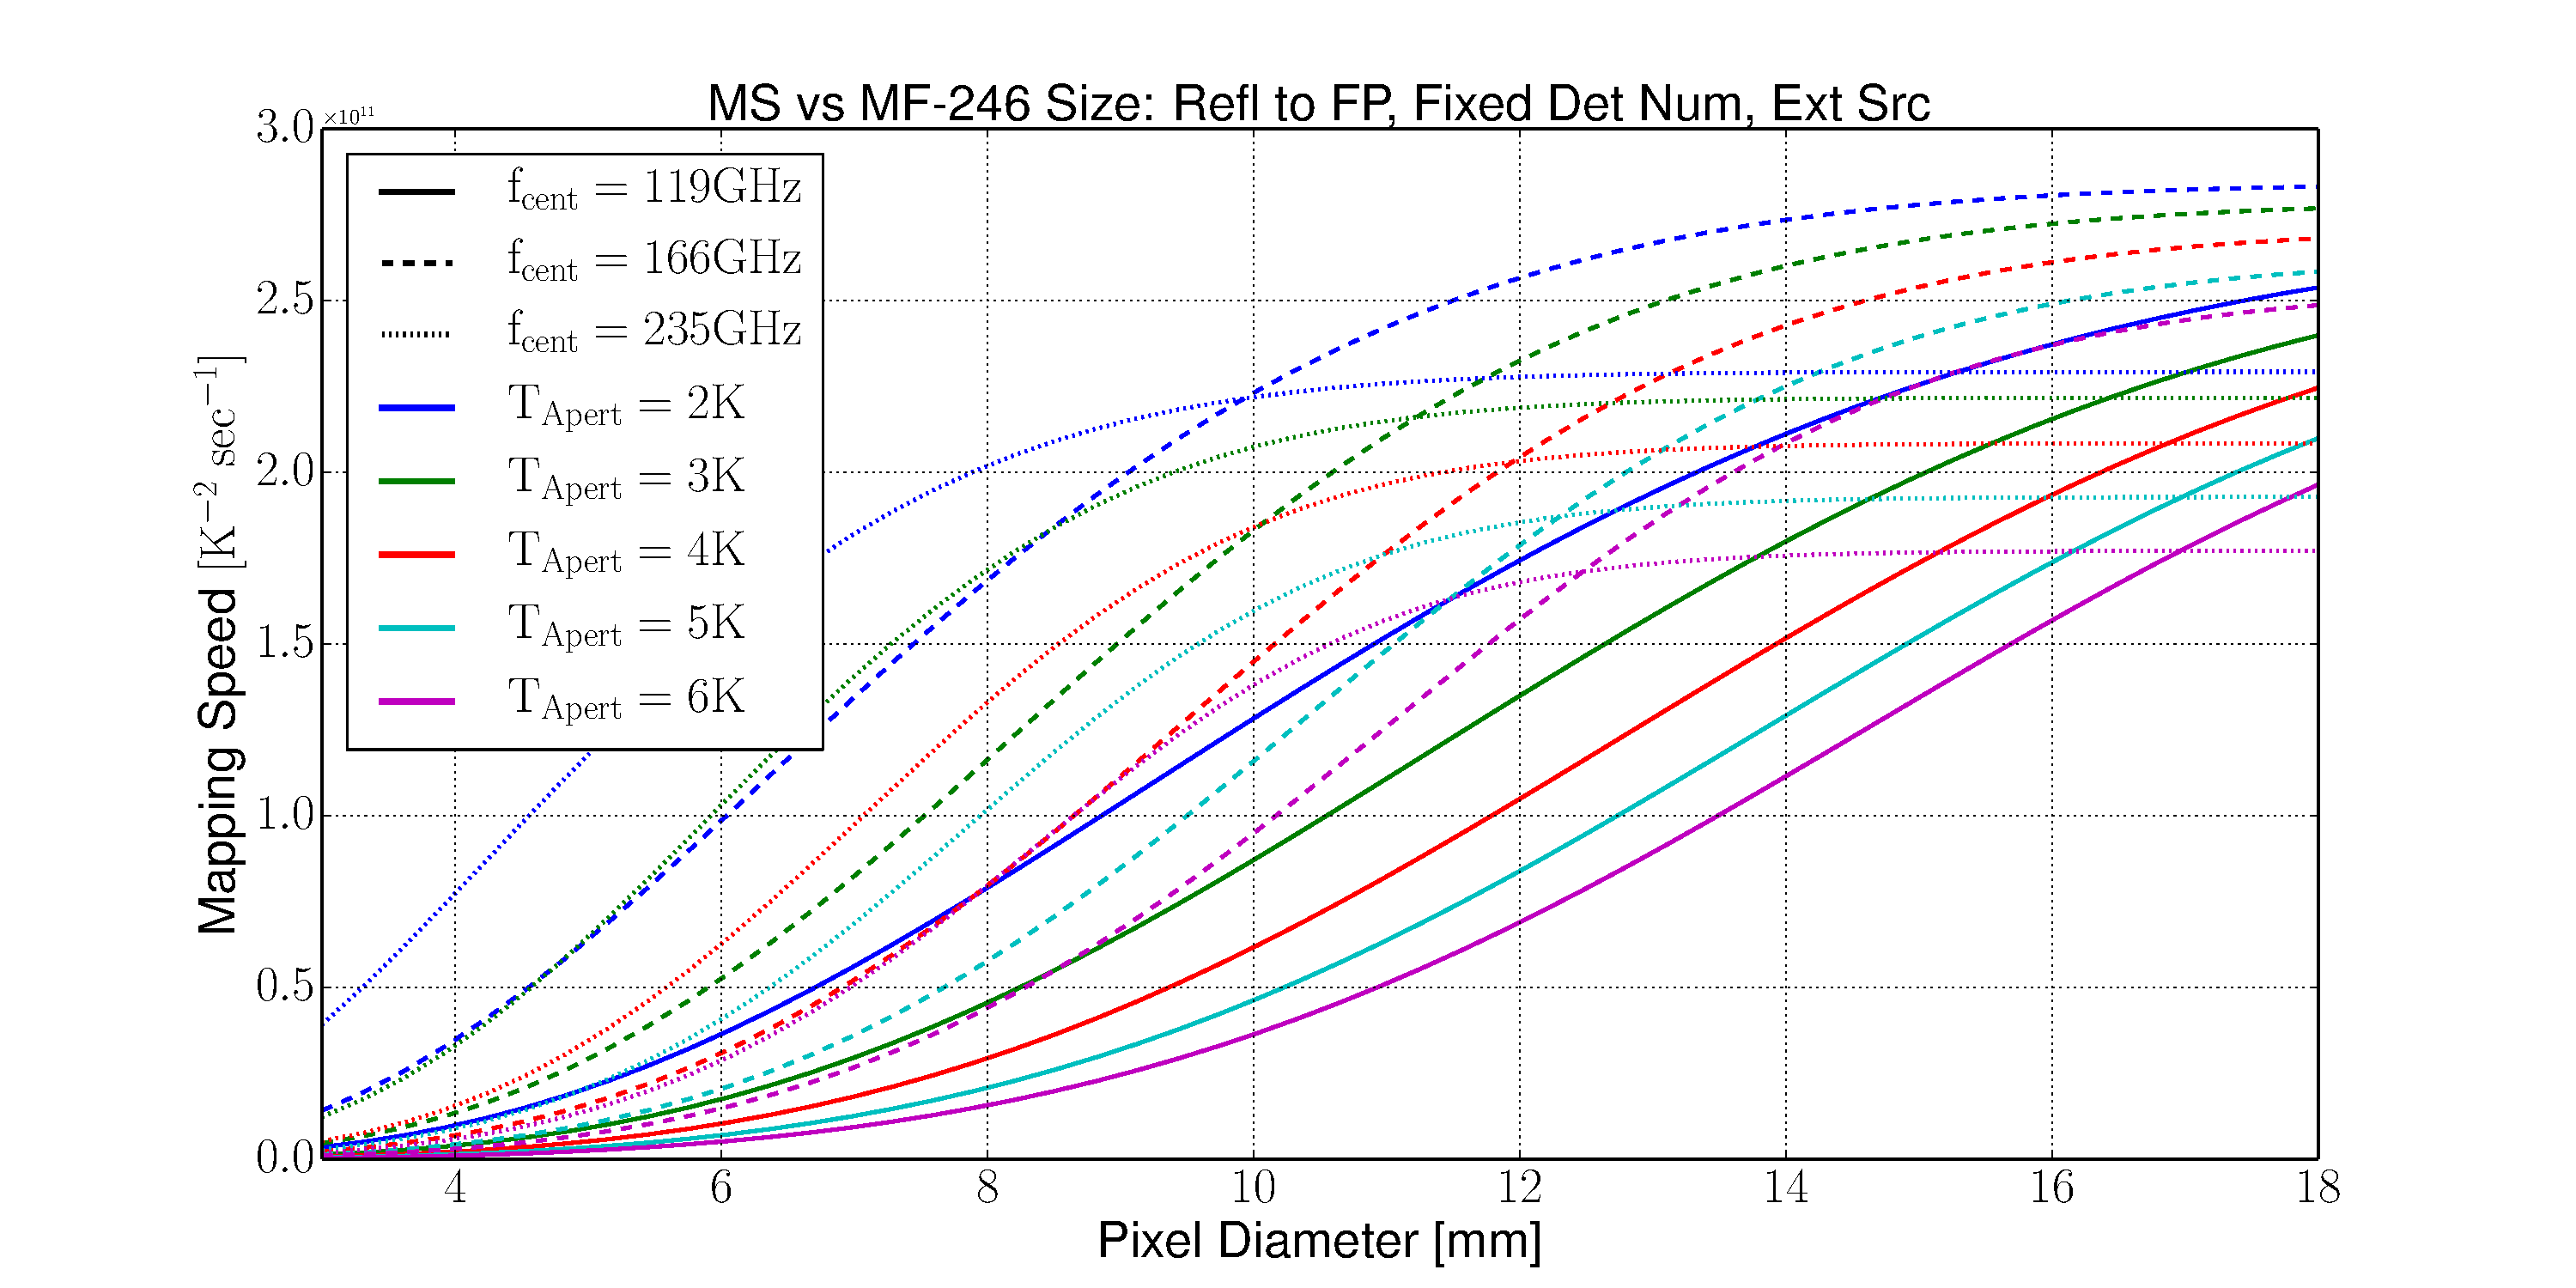
\includegraphics[width=1.1\textwidth, center]{PDF/LFT_MS_MF-246_coldRefl_fixDetNum_extSrc.pdf}
	\caption{MF-246 mapping speed of an extended source as a function of pixel diameter for cold reflections and fixed number of detectors}
\end{figure}

\begin{figure}[H]
	\centering
	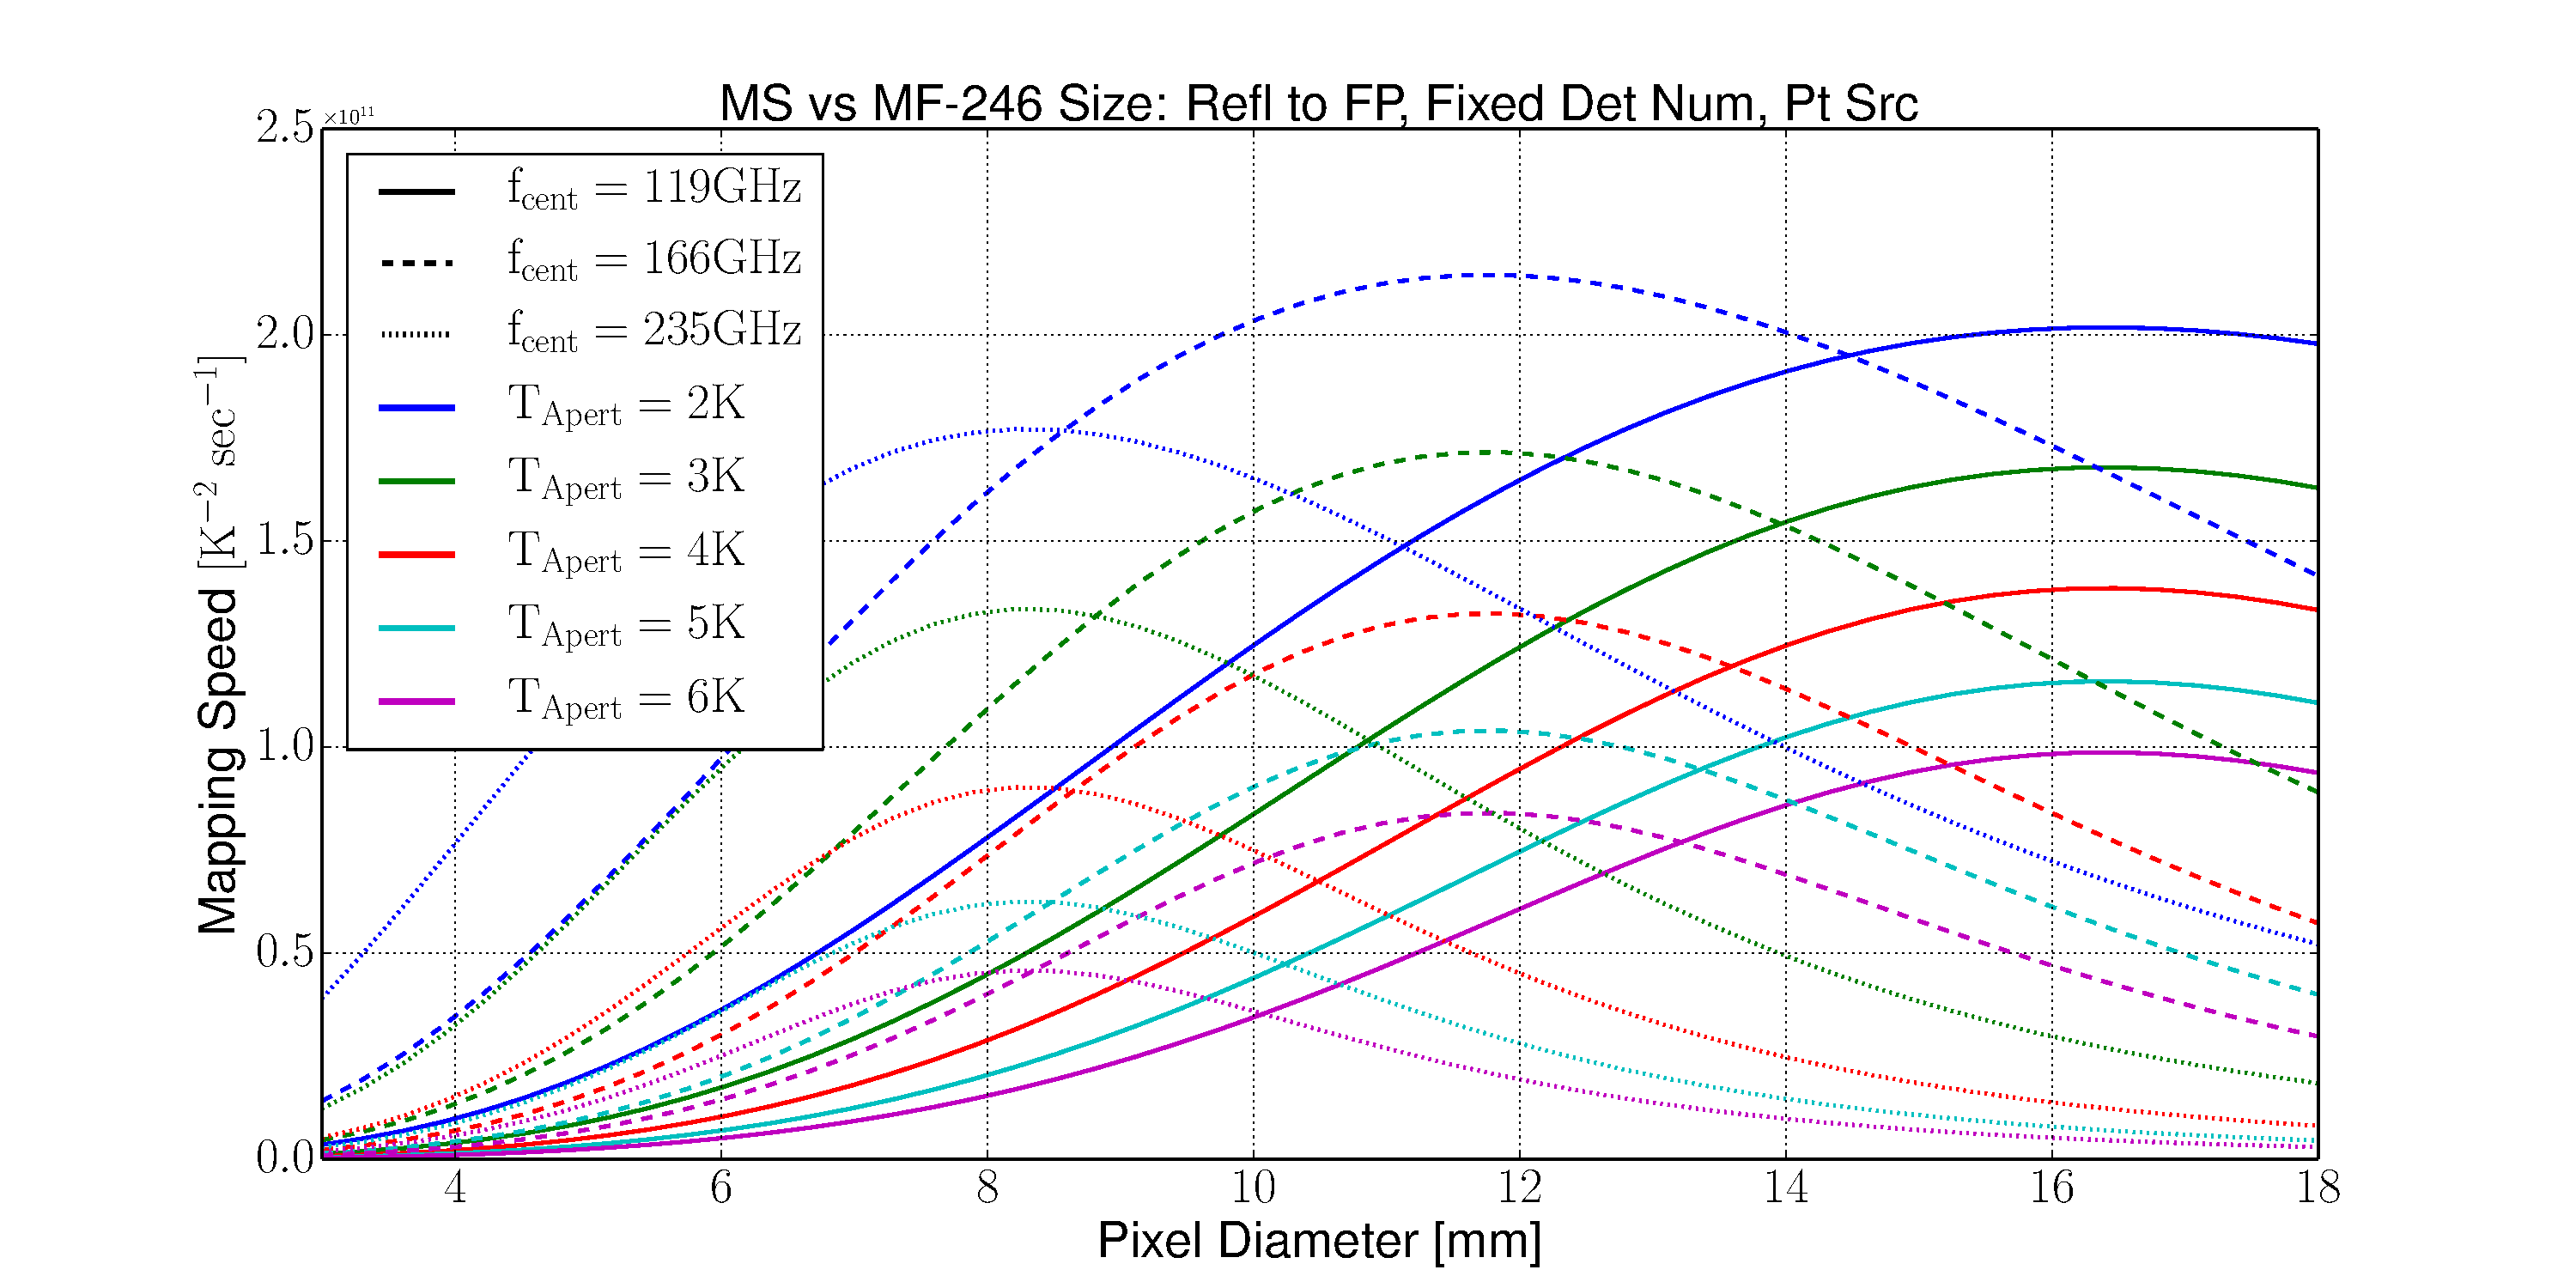
\includegraphics[width=1.1\textwidth, center]{PDF/LFT_MS_MF-246_coldRefl_fixDetNum_ptSrc.pdf}
	\caption{MF-246 mapping speed of a point source as a function of pixel diameter for cold reflections and fixed number of detectors}
\end{figure}

%%%%%%%%%%%%%%%%%%%

\subsubsection{HFT}

\begin{figure}[H]
	\centering
	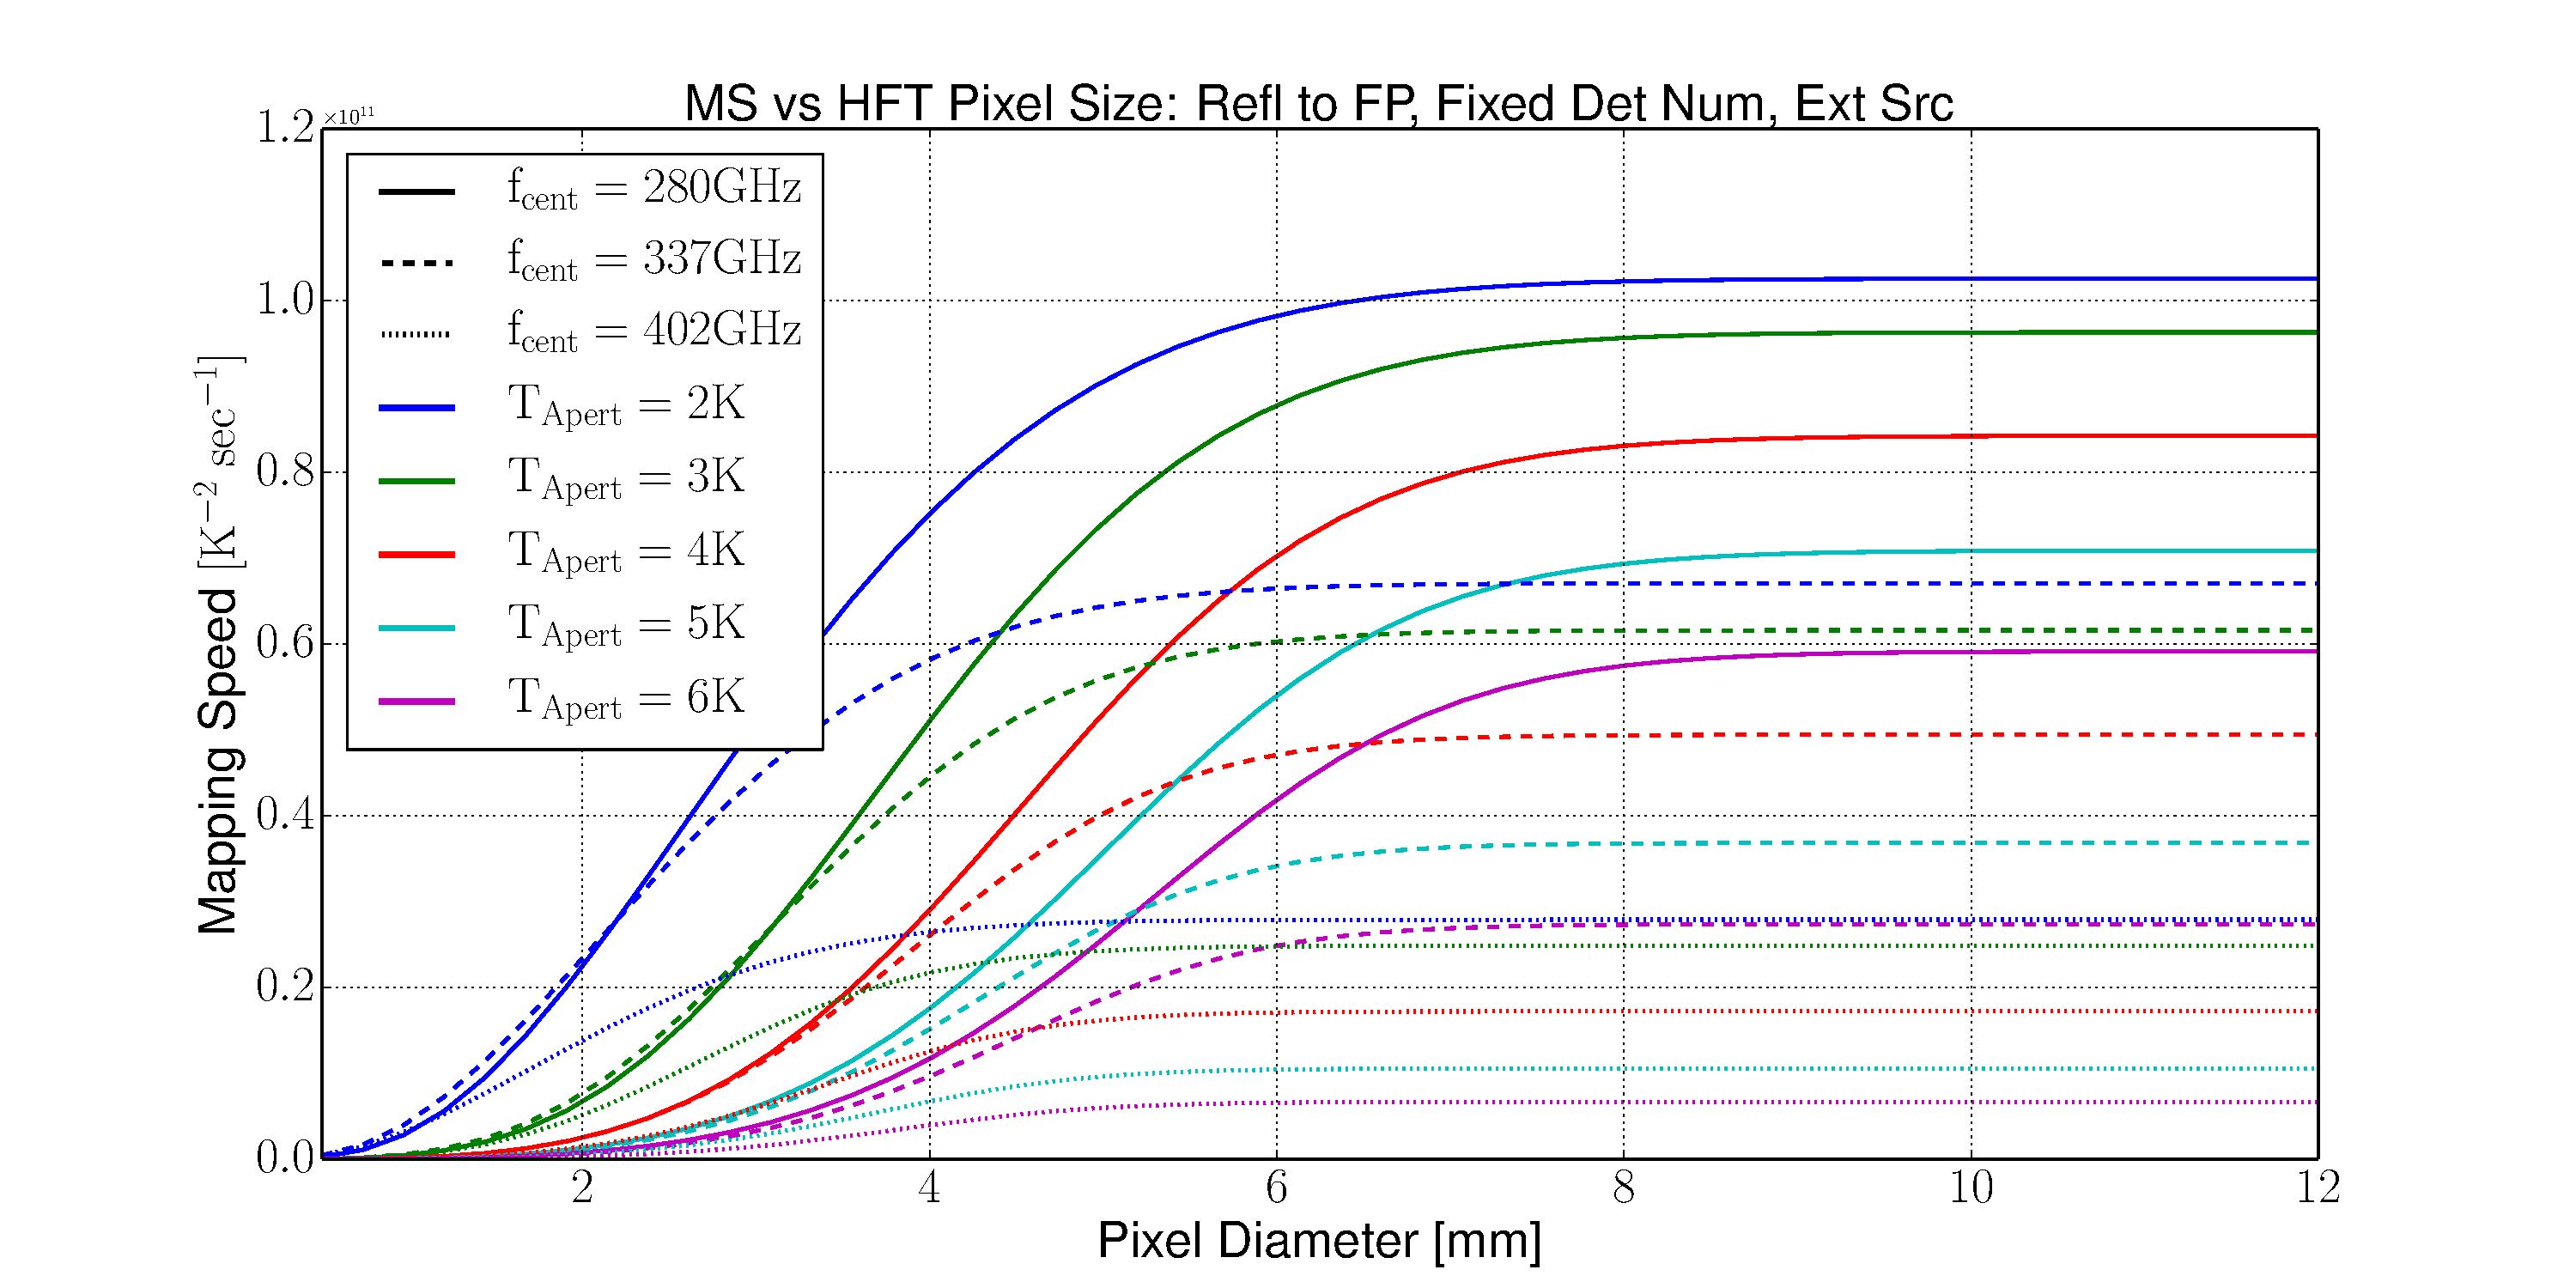
\includegraphics[width=1.1\textwidth, center]{PDF/HFT_MS_coldRefl_fixDetNum_extSrc.pdf}
	\caption{HFT mapping speed of an extended source as a function of pixel diameter for cold reflections and fixed number of detectors}
\end{figure}

\begin{figure}[H]
	\centering
	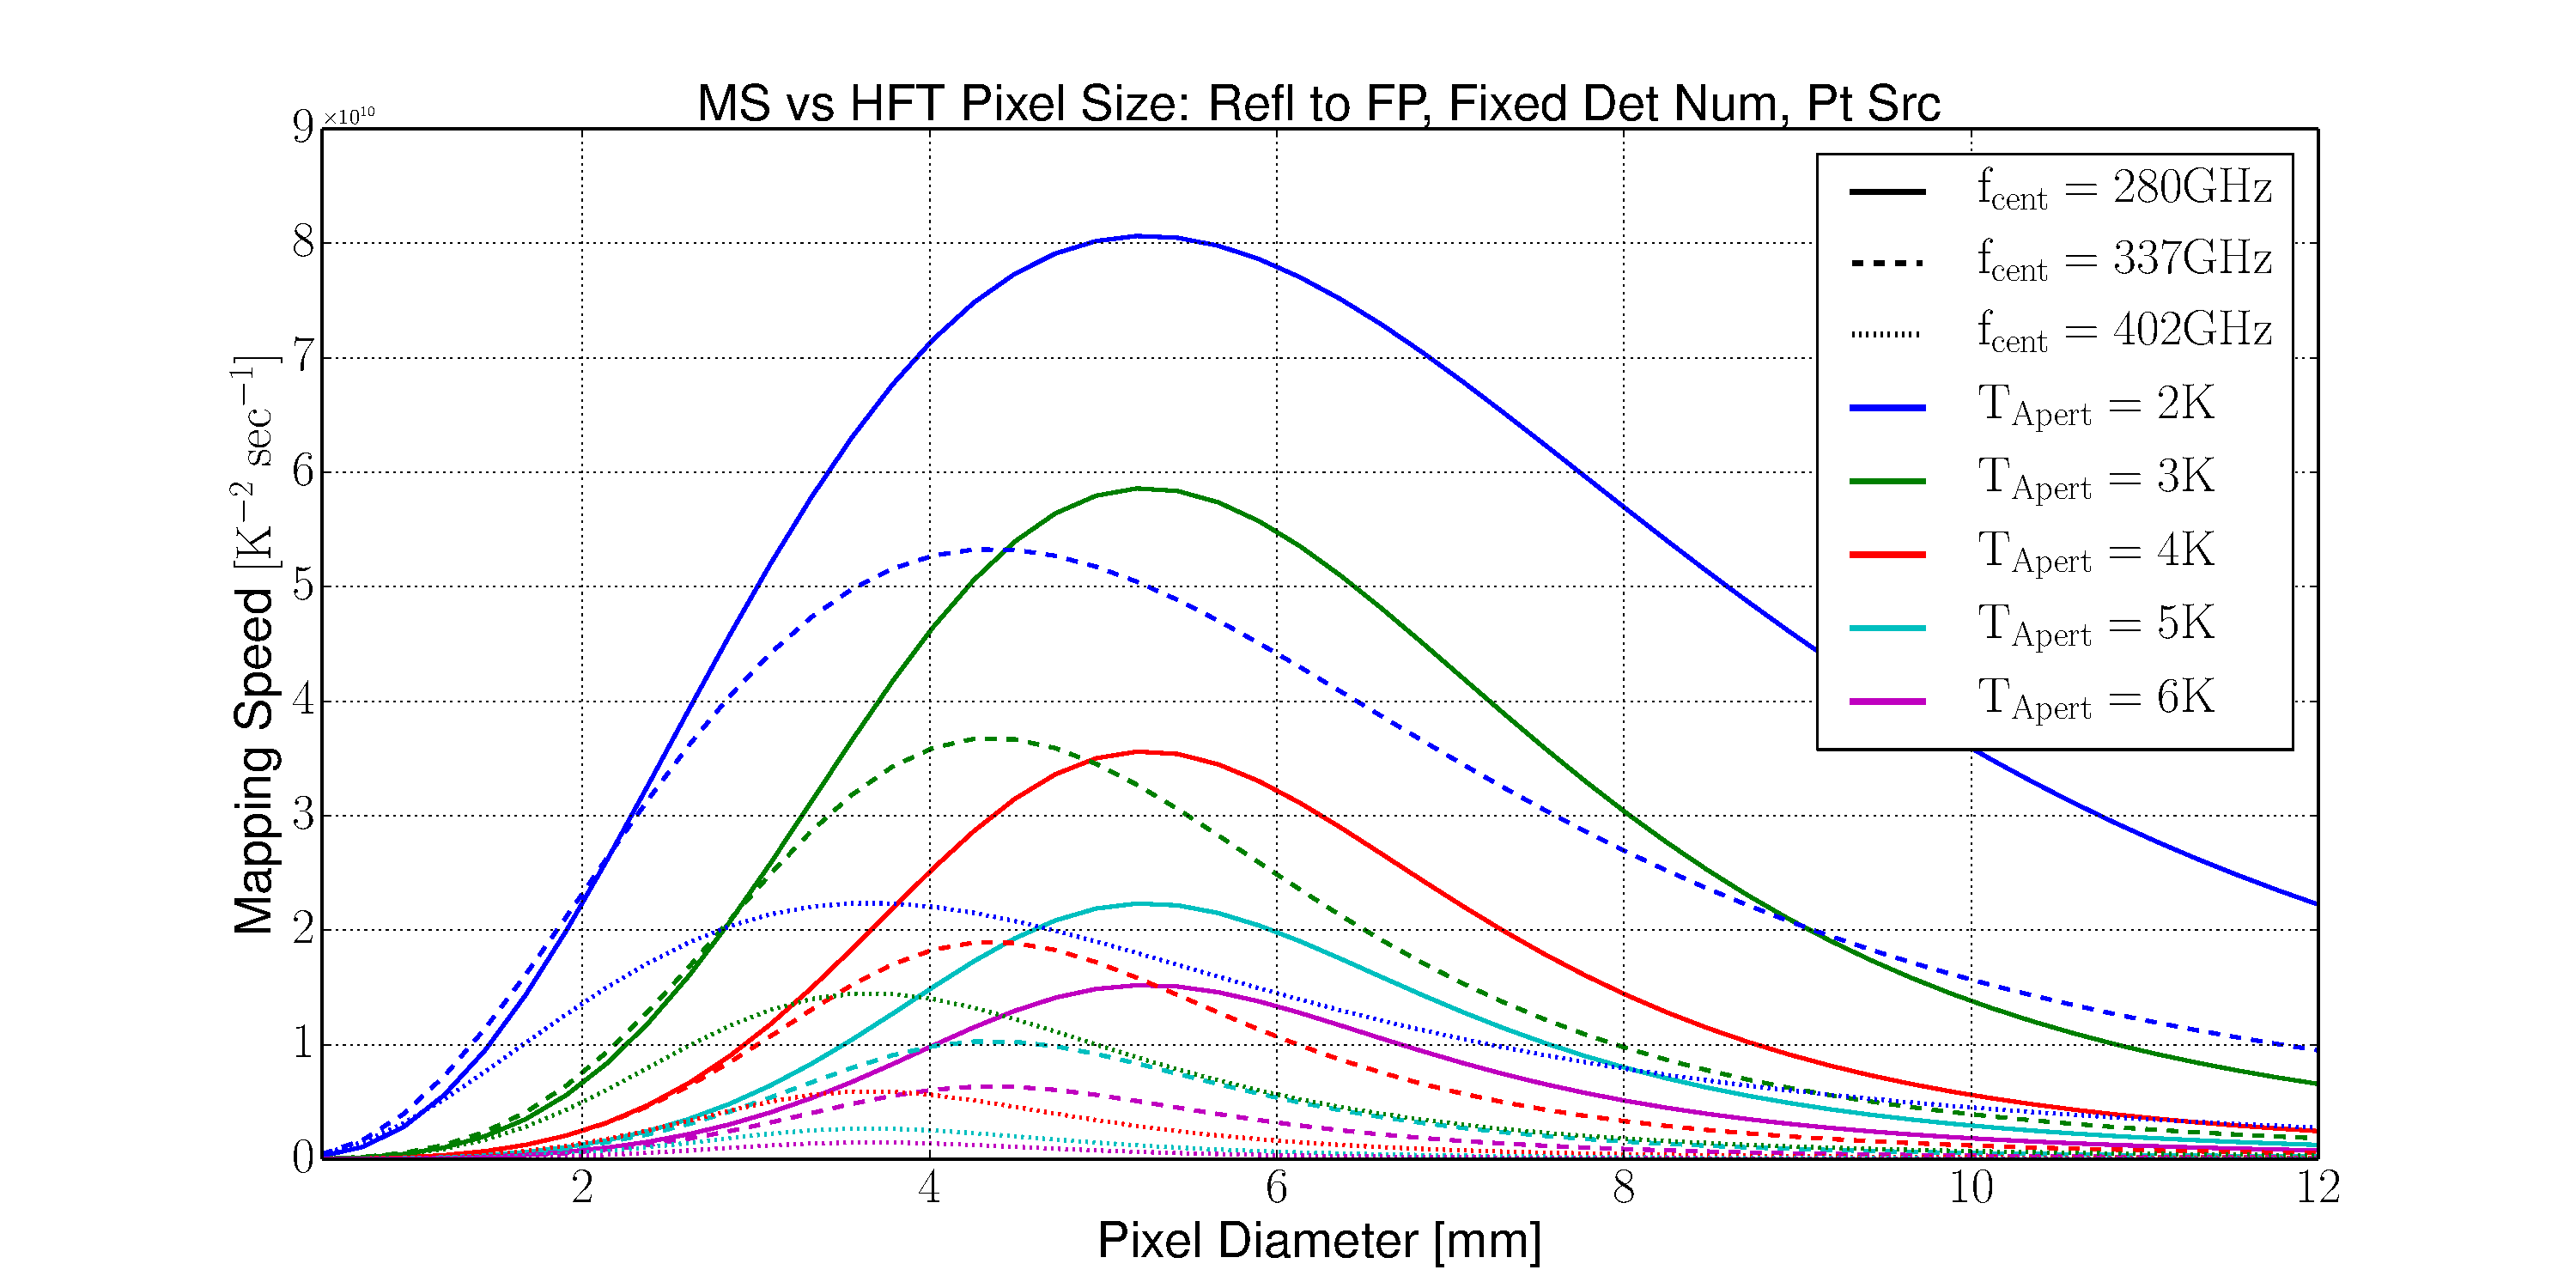
\includegraphics[width=1.1\textwidth, center]{PDF/HFT_MS_coldRefl_fixDetNum_ptSrc.pdf}
	\caption{HFT mapping speed of a point source as a function of pixel diameter for cold reflections and fixed number of detectors}
\end{figure}

%%%%%%%%%%%%%%%%%%%%%%%%%%%%%%%%%%%%%

\subsection{Summary of Optimal Diameters \label{subsec:OptDiams}}

Table \ref{table:optDiamsAssumps} describes the assumptions that we take in this document when identifying the optimal pixel diameters for each frequency channel.

\begin{table}[H]
\centering
	\begin{tabularx}{\textwidth}{|| X | X | X ||}
	\hline
	Parameter & Assumed Value & Comment \\ 	
	\hline
	\hline
	Baffle Temperature & 5 K & Helium-cooled \\
	\hline
	Aperture Temperature & 5 K & Helium-cooled \\
	\hline
	Focal Plane Limitation & FOV-limited & Cannot push Strehl's, payload, fabrication cost, etc \\
	\hline
	Reflections & Land on baffle & Most conservative assumption \\
	\hline
	Observation Source & Extended & We are primarily interested in the CMB \\
	\hline
	\end{tabularx}
\caption{Assumptions behind finding optimal pixel diameters \label{table:optDiamsAssumps}}
\end{table}

\textbf{NOTE THAT THE OPTIMAL PIXEL DIAMETERS LAYED OUT IN THIS SECTION ARE LEFTOVER FROM BEFORE THE BAFFLE MOVED TO 2 K AND THEREFORE SHOULD BE UPDATED}. We may be in a regime where we are readout-limited, but if not, then we can perhaps pack more detectors onto the focal plane using smaller pixel diameters for enhanced mapping speed.

Given these assumptions in the above table, Table \ref{table:sumOptPixDiams} shows the optimal pixel diameter for each frequency channel.

Because we have three channels on each triplexed pixel, it is prudent to choose one frequency to favor over the other two. For this analysis, we aim to maximize sensitivity on the channels that receive the most CMB power. I've boldfaced the frequency channel that I think should determine the each pixel's diameter.

\begin{table}[H]
\centering
	\begin{tabu}{|| c | c ||}
	\hline
	Band & Optimal Pixel Diameter [mm] \\	
	\hline
	\hline
	\multicolumn{2}{|| c ||}{LF-135} \\
	\hline
	LF-1 & 37.0 \\
	\hline
	LF-3 & 24.5 \\
	\hline
	\textbf{LF-5} & \textbf{19.4} \\
	\hline
	\multicolumn{2}{|| c ||}{LF-246} \\
	\hline
	LF-2 & 29.9 \\	
	\hline
	LF-4 & 21.9 \\	
	\hline
	\textbf{LF-6} & \textbf{16.6} \\	
	\hline
	\multicolumn{2}{|| c ||}{MF-135} \\	
	\hline
	MF-1 & 15.0 \\
	\hline
	\textbf{MF-3} & \textbf{10.9} \\	
	\hline
	MF-5 & 8.1 \\	
	\hline
	\multicolumn{2}{|| c ||}{MF-246} \\	
	\hline
	MF-2 & 12.8 \\
	\hline
	\textbf{MF-4} & \textbf{9.4} \\	
	\hline
	MF-6 & 6.7 \\
	\hline
	\multicolumn{2}{|| c ||}{HFT} \\	
	\hline
	\textbf{HF-1} & \textbf{4.3} \\
	\hline
	\textbf{HF-2} & \textbf{3.6} \\	
	\hline
	\textbf{HF-3} & \textbf{3.1} \\
	\hline
	\end{tabu}
\caption{Summary of optimal pixel diameters \label{table:sumOptPixDiams}}
\end{table}

%%%%%%%%%%%%%%%%%%%%%%%%%%%%%%%%%%%%%

\subsection{Choosing Pixel Diameters}

Given the discussion of Section \ref{subsec:OptDiams}, we now must choose our pixel diameters. There are a few considerations whe making this decision:

\begin{enumerate}
	\item Quantization of hexagonal wafer division
	\item Minimum allowed diameter for the lowest frequency channel on each pixel
	\item Maximum allowed diameter given a finite wafer size and number of pixels on that wafer
\end{enumerate}

We will take a brief look at all of these considerations in the following sections.

%%%%%%%%%%%%%%%%%%%

\subsubsection{Hexagon Quantization and Maximum Pixel Diameter}

Assuming a 110mm hexagonal wafer, Figure \ref{fig:hexQuant} shows the allowed pixel configurations, their pixel count, and the maximum allowed pixel diameter allowed by that configuration.

\begin{figure}[H]
	\centering
	
	\begin{subfigure}{0.3\textwidth}
		\centering
		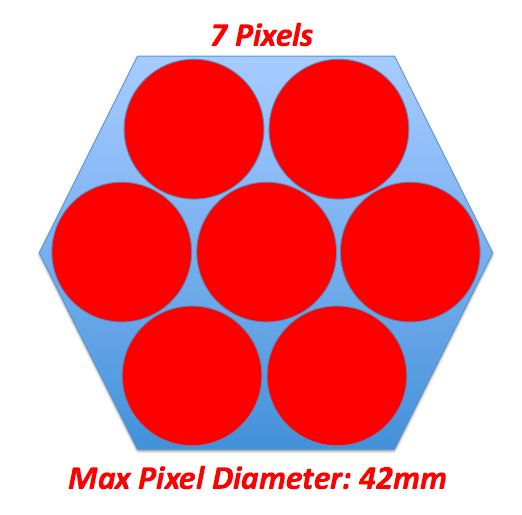
\includegraphics[width=\linewidth]{PNG/7pixels}
	\end{subfigure}%	
	\begin{subfigure}{0.3\textwidth}
		\centering
		\includegraphics[width=\linewidth]{PNG/19pixels}
	\end{subfigure}%
	\begin{subfigure}{0.3\textwidth}
		\centering
		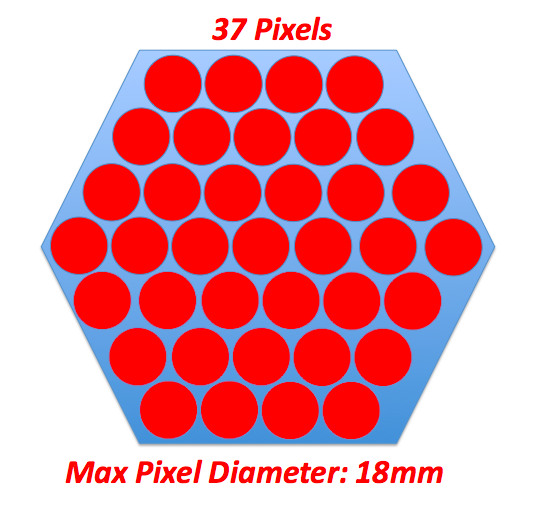
\includegraphics[width=\linewidth]{PNG/37pixels}
	\end{subfigure} \\
	
	\begin{subfigure}{0.5\textwidth}
		\centering
		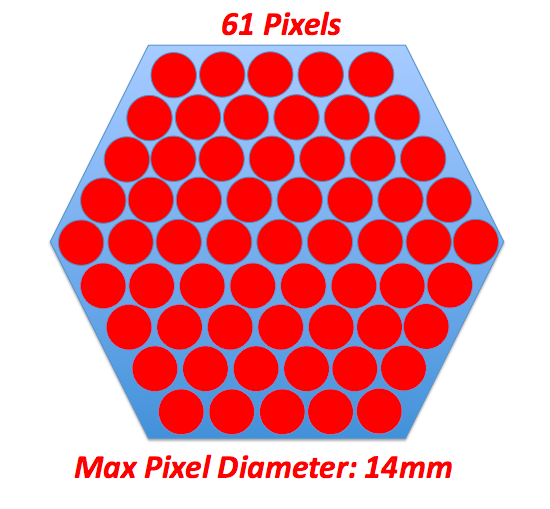
\includegraphics[width=\linewidth]{PNG/61pixels}
	\end{subfigure}%
	\begin{subfigure}{0.5\textwidth}
		\centering
		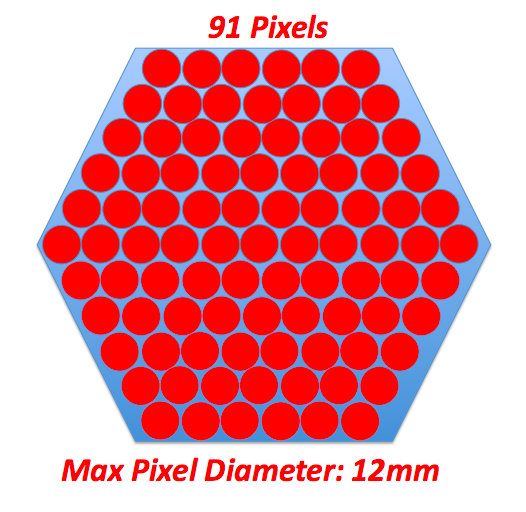
\includegraphics[width=\linewidth]{PNG/79pixels}
	\end{subfigure}
	
\caption{Allowed pixel configurations and their maximum allowed diameters assuming that the host wafer is 110mm side-to-side \label{fig:hexQuant}}
\end{figure}

%%%%%%%%%%%%%%%%%%%

\subsection{Lenslet Focusing and Minimum Pixel Diameter}

In order for a lenslet to have adequate focusing power, its diameter needs to obey the relation

\begin{equation}
	D \geq 2 \, \lambda_{0}
\end{equation}

where $\lambda_{0}$ is the wavelength of the incident radiation in a vacuum. Given this constraint, we can set a lower bound on the allowed diameter of each pixel by considering the lowest edge of its lowest frequency band. 

Note that these minimum values only apply to LFT pixels.

\begin{table}[H]
\centering
	\begin{tabu}{|| c | c | c ||}
	\hline
	Pixel & Lowest Frequency [GHz] & Minimum Diameter [mm] \\
	\hline
	\hline
	LF-135 & 34 & 18 \\
	\hline
	LF-246 & 43 & 14 \\
	\hline
	MF-135 & 85 & 7.1 \\
	\hline
	MF-246 & 101 & 5.9 \\
	\hline
	\end{tabu}
\caption{Minimum allowed diameters for LFT pixels \label{table:minAllowDiams}}
\end{table}

%%%%%%%%%%%%%%%%%%%

\subsection{Pixel Diameters for this Document}

Given the constraints laid out in this section, we take the pixel diameters listed in Table \ref{table:actualPixSizes}.

\begin{table}[H]
\centering
	\begin{tabu}{|| c | c ||}
	\hline
	Pixel & Diameter [mm] \\
	\hline
	\hline
	LF-135 & 18 \\
	\hline
	LF-246 & 18 \\
	\hline
	MF-135 & 12 \\
	\hline
	MF-246 & 12 \\
	\hline
	HF-1 & 5.4 \\
	\hline
	HF-2 & 4.5 \\
	\hline
	HF-3 & 4.0 \\
	\hline
	\end{tabu}
\caption{Pixel sizes used in this document \label{table:actualPixSizes}}
\end{table}


Note that at the lower frequencies, the mapping speed is a slower function of pixel diameter than at higher frequencies. Therefore, we don't suffer so much by deploying the LF pixels below optimal diameter.


%%%%%%%%%%%%%%%%%%%%%%%%%%%%%%%%%%%%%%%%%%%%%%%%%%%%%%%%%%%%%%%%%%%%%%

\newpage

\section{Discussions}

\textbf{NOTE: These studies are old and need to be updated to take a 2 K aperture into account}.

This is the "grab bag" section that includes topics not directly related to the sensitivity calculation.

%%%%%%%%%%%%%%%%%%%

\subsection{Range of Possible Optical Loading \label{sec:possibleLoadings}}

It is important to understand the range of optical loading values that lie withint the realm of possibility for LiteBIRD. According to the assertions in this document, the "extreme" scenarios (code name "S\#"), listed from smallest expected photon loading to largest, are

\begin{itemize}
	\item[] \textbf{S1}: Reflections to focal plane, 4.5K baffling temperature
	\item[] \textbf{S2}: Reflections to baffling, 4.5K baffling temperature
	\item[] \textbf{S3}: Reflections to focal plane, 6.0K baffling temperature	
	\item[] \textbf{S4}: Reflections to baffling, 6.0K baffling temperature
\end{itemize}

In Table \ref{table:extremeLoading}, we list the in-band loading values for every frequency channel in each of the above scenarios.

\begin{table}[H]
\centering
	\begin{tabu}{|| c | c | c | c | c ||}
	\hline
	Band & \multicolumn{4}{c ||}{$\mathrm{P_{opt}}$ [pW]} \\
	\hline
	 & S1 & S2 & S3 & S4 \\
	\hline
	\hline
	LF-1 & 0.32 & 0.33 & 0.43 & 0.44 \\
	\hline
	LF-2 & 0.34 & 0.36 & 0.46 & 0.48 \\
	\hline
	LF-3 & 0.27 & 0.29 & 0.35 & 0.38 \\
	\hline
	LF-4 & 0.26 & 0.29 & 0.34 & 0.38 \\
	\hline
	LF-5 & 0.25 & 0.29 & 0.32 & 0.36 \\
	\hline
	LF-6 & 0.24 & 0.28 & 0.29 & 0.35 \\
	\hline
	MF-1 & 0.31 & 0.34 & 0.42 & 0.46 \\
	\hline
	MF-2 & 0.35 & 0.40 & 0.46 & 0.54 \\
	\hline
	MF-3 & 0.29 & 0.35 & 0.37 & 0.47 \\
	\hline
	MF-4 & 0.22 & 0.29 & 0.27 & 0.39 \\
	\hline
	MF-5 & 0.17 & 0.24 & 0.20 & 0.32 \\
	\hline
	MF-6 & 0.12 & 0.18 & 0.14 & 0.26 \\
	\hline
	HF-1 & 0.12 & 0.15 & 0.19 & 0.26 \\
	\hline
	HF-2 & 0.08 & 0.11 & 0.16 & 0.22 \\
	\hline
	HF-3 & 0.04 & 0.05 & 0.08 & 0.12 \\
	\hline
	\end{tabu}
\caption{In-band loading for extreme scenarios \label{table:extremeLoading}}
\end{table}

In Table \ref{table:extremeLoadingNoise}, we list the photon noise values for every frequency channel in each of the above scenarios.

\begin{table}[H]
\centering
	\begin{tabu}{|| c | c | c | c | c ||}
	\hline
	Band & \multicolumn{4}{c ||}{$\mathrm{NEP_{ph}}$ [aW/$\mathrm{\sqrt{Hz}}$]} \\
	\hline
	 & S1 & S2 & S3 & S4 \\
	\hline
	\hline
	LF-1 & 5.82 & 5.97 & 7.31 & 7.51 \\
	\hline
	LF-2 & 6.20 & 6.43 & 7.61 & 7.94 \\
	\hline
	LF-3 & 5.63 & 5.92 & 6.75 & 7.15 \\
	\hline
	LF-4 & 5.72 & 6.08 & 6.72 & 7.22 \\
	\hline
	LF-5 & 5.77 & 6.22 & 6.61 & 7.24 \\
	\hline
	LF-6 & 5.78 & 6.32 & 6.45 & 7.23 \\
	\hline
	MF-1 & 6.97 & 7.38 & 8.36 & 8.94 \\
	\hline
	MF-2 & 7.85 & 8.48 & 9.20 & 10.1 \\
	\hline
	MF-3 & 7.57 & 8.38 & 8.63 & 9.85 \\
	\hline
	MF-4 & 7.13 & 8.15 & 7.88 & 9.50 \\
	\hline
	MF-5 & 6.64 & 7.87 & 7.17 & 9.22 \\
	\hline
	MF-6 & 6.04 & 7.47 & 6.51 & 9.04 \\
	\hline
	HF-1 & 6.73 & 7.54 & 8.47 & 9.90 \\
	\hline
	HF-2 & 6.03 & 6.86 & 8.30 & 9.81 \\
	\hline
	HF-3 & 4.34 & 5.07 & 6.60 & 8.00 \\
	\hline
	\end{tabu}
\caption{Photon noise for extreme scenarios \label{table:extremeLoadingNoise}}
\end{table}

%%%%%%%%%%%%%%%%%%%

\subsection{Effect of Optical Element Temperatures on Sensitivity}

The following plots show the effect of the temperature of the optical elements shown in Table \ref{table:effectOfTemp} on LB sensitivity, both band-by-band and for the instrumet as a whole.

\begin{table}[H]
\centering
	\begin{tabu}{||c | c ||}
	\hline
	Optical Element & Temperature Range [K] \\
	\hline
	\hline
	Baffle & 4.5 - 6.5 \\
	\hline
	HWP & 4.5 - 6.5 \\
	\hline
	Aperture & 4.5 - 6.5 \\
	\hline
	Mirrors (LFT)/Lenses (HFT) & 4.5 - 6.5 \\
	\hline
	\end{tabu}
\caption{Optical elements whose temperature depends on 4K fridge performance \label{table:effectOfTemp}}
\end{table}

%%%%%%%%%%

\subsubsection{Effect of Baffle Temperature}

\begin{figure}[H]
	\centering
	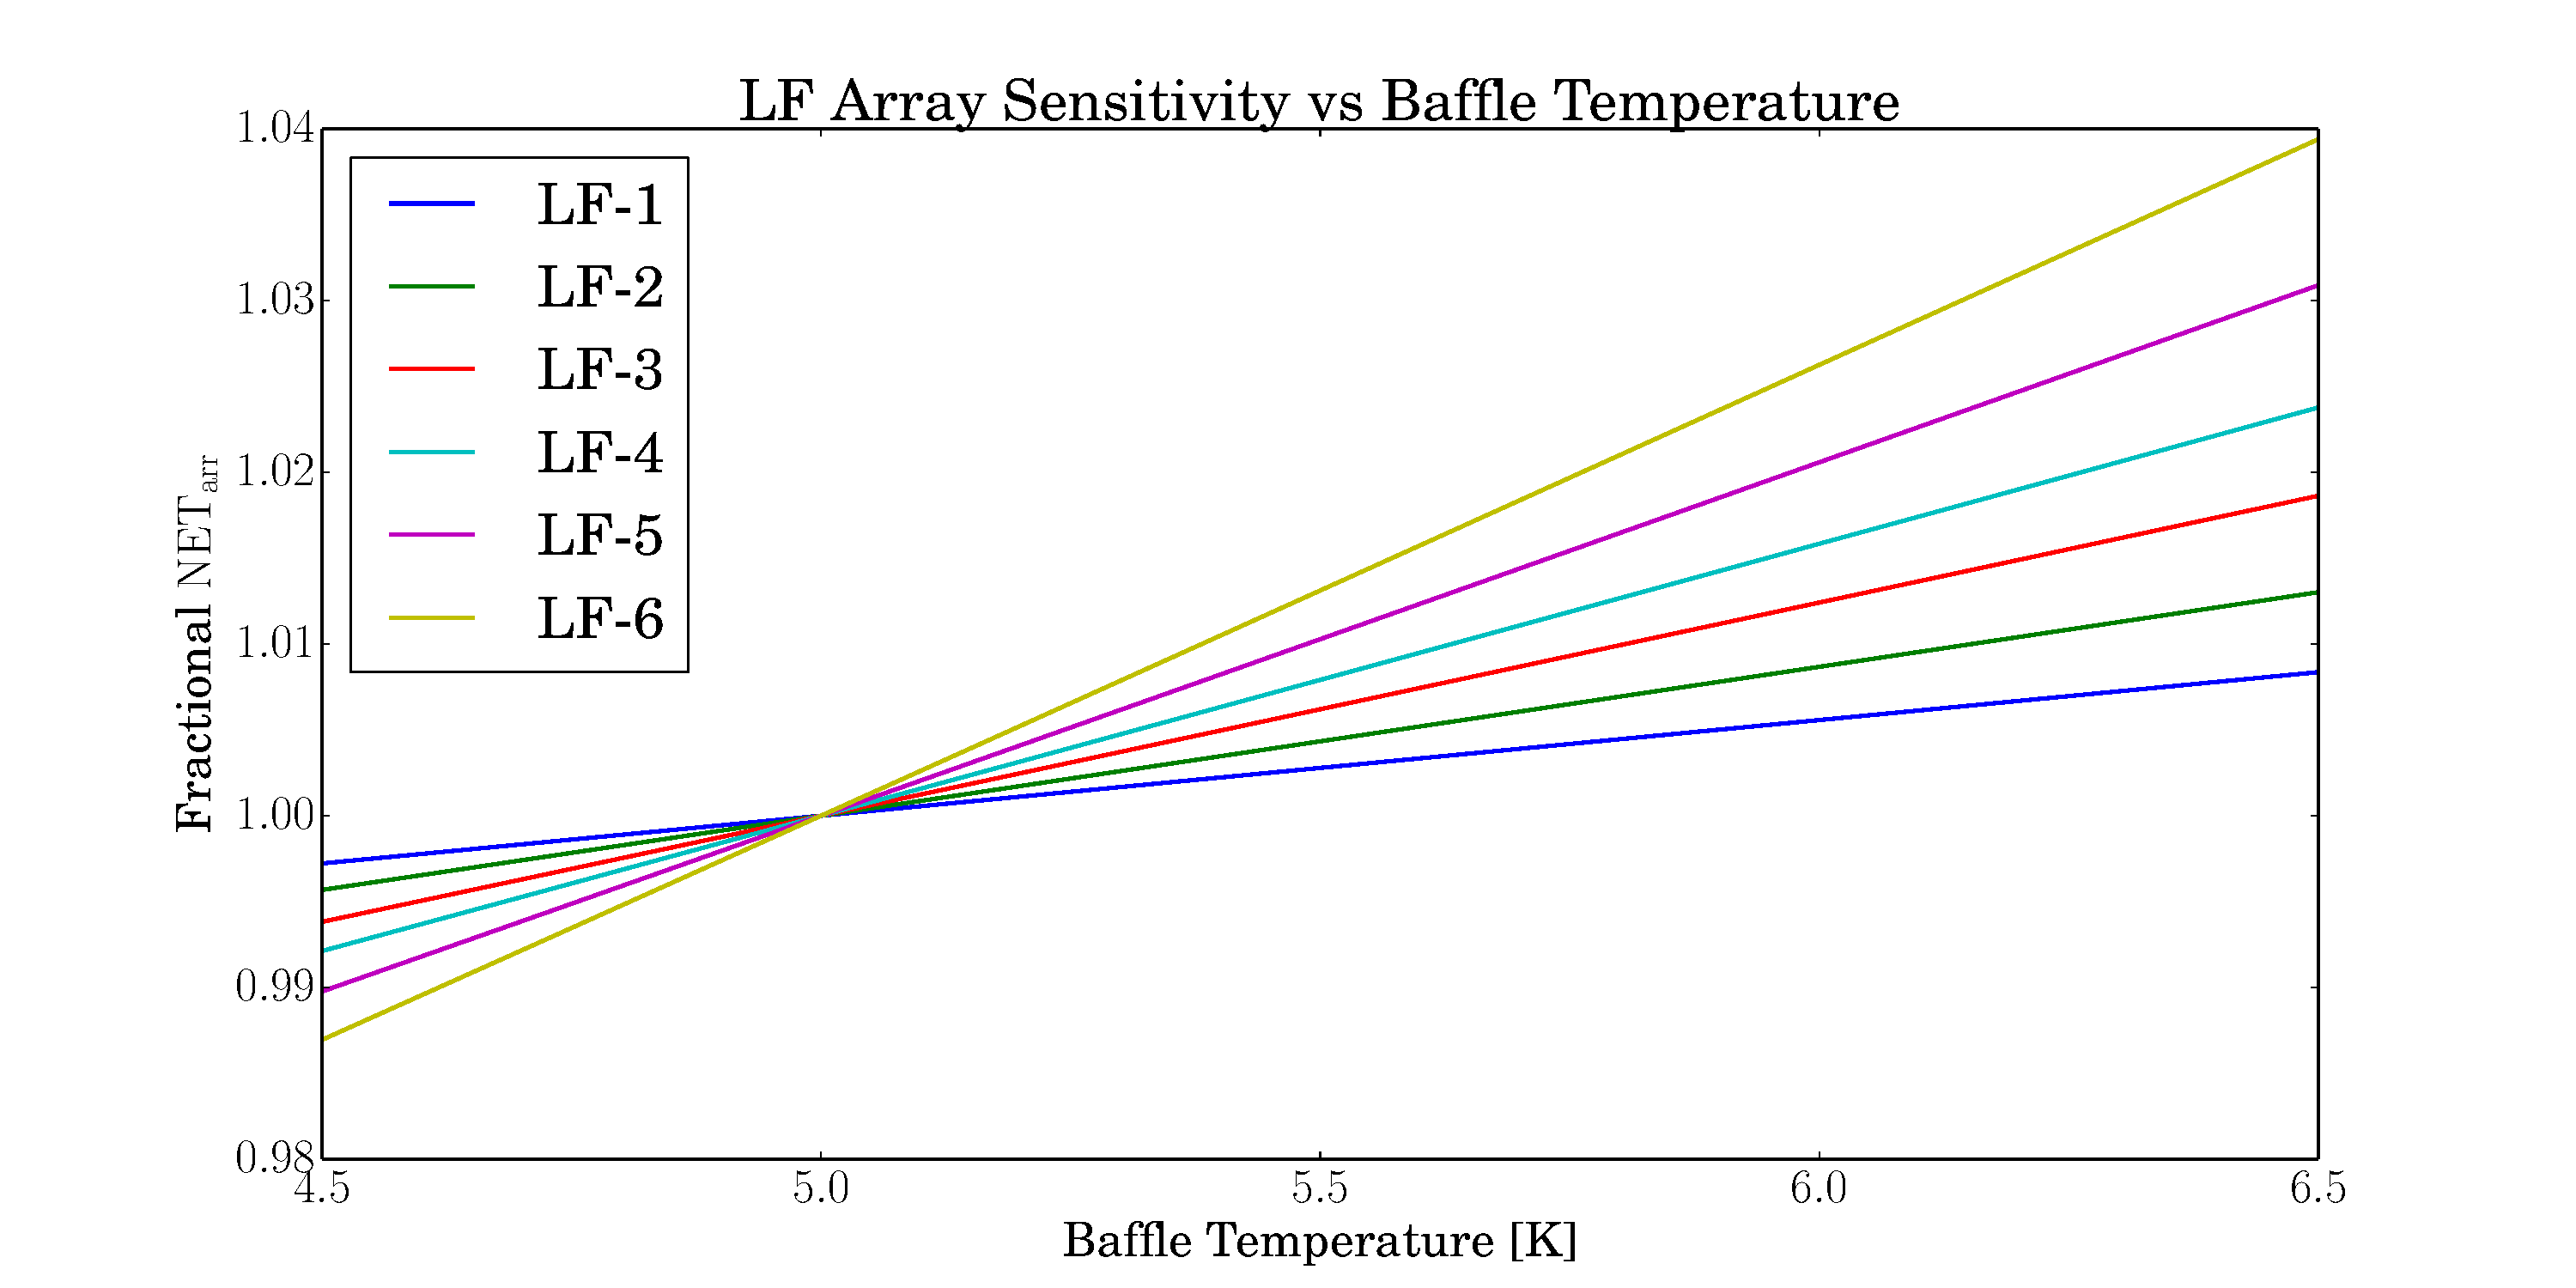
\includegraphics[width=1.1\textwidth, center]{PDF/TempDependence_Baffle_LF.pdf}
	\caption{LF Array sensitivity vs Baffle temperature}
\end{figure}

\begin{figure}[H]
	\centering
	\includegraphics[width=1.1\textwidth, center]{PDF/TempDependence_Baffle_MF.pdf}
	\caption{MF Array sensitivity vs Baffle temperature}
\end{figure}
	
\begin{figure}[H]
	\centering
	\includegraphics[width=1.1\textwidth, center]{PDF/TempDependence_Baffle_HF.pdf}
	\caption{HF Array sensitivity vs Baffle temperature}
\end{figure}

\begin{figure}[H]
	\centering
	\includegraphics[width=1.1\textwidth, center]{PDF/TempDependence_Baffle_LB.pdf}
	\caption{LB sensitivity vs Baffle temperature}
\end{figure}

%%%%%%%%%%

\subsubsection{Effect of HWP Temperature}

\begin{figure}[H]
	\centering
	\includegraphics[width=1.1\textwidth, center]{PDF/TempDependence_HWP_LF.pdf}
	\caption{LF Array sensitivity vs HWP temperature}
\end{figure}

\begin{figure}[H]
	\centering
	\includegraphics[width=1.1\textwidth, center]{PDF/TempDependence_HWP_MF.pdf}
	\caption{MF Array sensitivity vs HWP temperature}
\end{figure}
	
\begin{figure}[H]
	\centering
	\includegraphics[width=1.1\textwidth, center]{PDF/TempDependence_HWP_HF.pdf}
	\caption{HF Array sensitivity vs HWP temperature}
\end{figure}

\begin{figure}[H]
	\centering
	\includegraphics[width=1.1\textwidth, center]{PDF/TempDependence_HWP_LB.pdf}
	\caption{LB sensitivity vs HWP temperature}
\end{figure}

%%%%%%%%%%

\subsubsection{Effect of Aperture Temperature}

\begin{figure}[H]
	\centering
	\includegraphics[width=1.1\textwidth, center]{PDF/TempDependence_Aperture_LF.pdf}
	\caption{LF Array sensitivity vs Aperture temperature}
\end{figure}

\begin{figure}[H]
	\centering
	\includegraphics[width=1.1\textwidth, center]{PDF/TempDependence_Aperture_MF.pdf}
	\caption{MF Array sensitivity vs Aperture temperature}
\end{figure}
	
\begin{figure}[H]
	\centering
	\includegraphics[width=1.1\textwidth, center]{PDF/TempDependence_Aperture_HF.pdf}
	\caption{HF Array sensitivity vs Aperture temperature}
\end{figure}

\begin{figure}[H]
	\centering
	\includegraphics[width=1.1\textwidth, center]{PDF/TempDependence_Aperture_LB.pdf}
	\caption{LB sensitivity vs Aperture temperature}
\end{figure}

%%%%%%%%%%

\subsubsection{Effect of Mirror/Lens Temperature}

\begin{figure}[H]
	\centering
	\includegraphics[width=1.1\textwidth, center]{PDF/TempDependence_Mirror_LF.pdf}
	\caption{LF Array sensitivity vs Mirror temperature}
\end{figure}

\begin{figure}[H]
	\centering
	\includegraphics[width=1.1\textwidth, center]{PDF/TempDependence_Mirror_MF.pdf}
	\caption{MF Array sensitivity vs Mirror temperature}
\end{figure}
	
\begin{figure}[H]
	\centering
	\includegraphics[width=1.1\textwidth, center]{PDF/TempDependence_Lens_HF.pdf}
	\caption{HF Array sensitivity vs Lens temperature}
\end{figure}

\begin{figure}[H]
	\centering
	\includegraphics[width=1.1\textwidth, center]{PDF/TempDependence_MirrorLens_LB.pdf}
	\caption{LB sensitivity vs Mirror/Lens temperature}
\end{figure}

%%%%%%%%%%%%%%%%%%%

\subsection{Still To Do}

There are still many tasks to complete before this analysis can be taken seriously. This list of tasks includes

\begin{enumerate}
	\item Estimate external noise $\mathrm{NEP_{ext}}$ for each frequency channel
	\item Critically evaluate the sensitivity contingency we're giving ourselves, given all these possible sources and how much/little we know about them
	\item ...
\end{enumerate}


%%%%%%%%%%%%%%%%%%%%%%%%%%%%%%%%%%%%%%%%%%%%%%%%%%%%%%%%%%%%%%%%%%%%%%

\newpage

\begin{thebibliography}{9}

\bibitem{parshin}
V. V. Parshin et al.
\emph{Silicon as an Advanced Window Material for High Power Gyrotrons}.
\url{http://link.springer.com/article/10.1007\%2FBF02066662}

\bibitem{lamb}
James W. Lamb.
\emph{Miscellaneous Data on Materials for Millimetre and Submillimetre Optics}
\url{http://link.springer.com/article/10.1007\%2FBF02069487}

\bibitem{kasparek}
W. Kasparek et al.
\emph{Measurements of Ohmic Losses of Metallic Reflectors at 140 GHz Using a 3-Mirror Resonator Technique}
\url{http://link.springer.com/article/10.1023\%2FA\%3A1015064616703}

\bibitem{cardiff}
Peter Ade at al.
\emph{A Review of Metal Mesh Filters}
\url{http://asd.gsfc.nasa.gov/cosmology/spirit/tech\_papers/Ade\_filter\_review.pdf}

\bibitem{bolowikiMMF}
Aritoki Suzuki
\emph{350mK Metal Mesh Filter Band Pass Filter Analysis}
\url{https://bolowiki.berkeley.edu/twiki/bin/view/Main/PB2350mKMetalMeshBandAnalysis}

\bibitem{planckMirror}
S. Roose et al.
\emph{Design of the cryo-optical test of the Planck Reflectors}
\url{https://orbi.ulg.ac.be/bitstream/2268/82057/1/cryo-optical\%20test\%20of\%20the\%20planck\%20reflectors.pdf}

\bibitem{tokiThesis}
Aritoki Suzuki.
\emph{Multichroic Detector Architecture for Cosmic Microwave Background Polarimetry Experiments}
\url{http://search.proquest.com/docview/1526024558}

\bibitem{kamThesis}
Kam Arnold.
\emph{Design and Deployment of the Polarbear Cosmic Microwave BackgroundPolarization Experiment}
\url{http://escholarship.org/uc/item/99m8b32x\#page-1}

\bibitem{zmuidzinas}
Jonas Zmuidzinas.
\emph{Thermal noise and correlations in photon detection}
\url{http://www.submm.caltech.edu/~jonas/tex/papers/pdf/2003-APPLOPT-Zmuidzinas.pdf}

\bibitem{keatingBICEP}
Brian Keating.
\emph{BICEP: A Large Angular Scale CMB Polarimeter}
\url{http://bicep0.caltech.edu/public/bicep/BICEP\_color.pdf}

\bibitem{almaCorrugatedHorn}
A. Baryshev, W. Wild.
\emph{ALMA Band 9 Optical Layout}.
\url{http://legacy.nrao.edu/alma/memos/html-memos/alma394/memo394.pdf}

\end{thebibliography}

\end{document}
